\begin{filecontents}{shortbib.bib}
@misc{he2015deep,
      title={Deep Residual Learning for Image Recognition}, 
      author={Kaiming He and Xiangyu Zhang and Shaoqing Ren and Jian Sun},
      year={2015},
      eprint={1512.03385},
      archivePrefix={arXiv},
      primaryClass={cs.CV}
}
\end{filecontents}

\documentclass{article}
\usepackage[a4paper, margin=1in]{geometry}
\usepackage{graphicx} % Required for inserting images
\usepackage{biblatex}
\bibliography{shortbib}
\usepackage{hyperref}
\hypersetup{
    colorlinks=true, % Set this to true to remove the border
    linkcolor=black, % Color for internal links
    citecolor=black, % Color for citations
    }
\usepackage{listings}
\usepackage{blindtext}
\usepackage{cleveref}
\usepackage{subcaption}
\geometry{margin=25mm}
\begin{document}

\section{Encoding Software}
\label{sec: encoder}

To encode the loss less images into the respective codec for the experiment, several encoder where used.
\subsection{AVIF, JPEG and WebP}
\subsubsection{AVIF}
AVIF is a format that utilizes the AV1 video codec. The AV1 codec employs block-based predictive coding. In this method, the frame is broken down into smaller units. Those are then analyzed to predict repetitive motion and color data based on blocks that have been processed earlier. Once the prediction is made, the redundant data is removed from the block. 
To convert the image into a sum of cosine functions of different frequencies the Discrete Cosine Transform (DCT) is used.

\subsubsection{JPEG}
JPEG uses the Discrete Cosine Transform (DCT) to convert an image into a sum of cosine functions of different frequencies. After the DCT, the coefficients are quantized to reduce their precision, and then entropy coded to compress the resulting data. The entropy coding method used in JPEG is Huffman coding.

\subsubsection{WebP}
In WebP a similar compression mechanism to that of the VP8 codec is used. This involves segmenting the frame into smaller units. Each of those units motion and color information is predicted based on previously processed blocks. This prediction process allows for the removal of redundant data from each block. The remaining data is then transformed using the Discrete Cosine Transform (DCT).

For those encoders the python package pillow-avif-plugin and pillow was used. The additional pillow plugin can be installed via pip install pillow-avif-plugin. To encode a lossless image, the image is opened and save with a specific quality as seen in listing \ref{avif_1}. The quality parameter ranges from 1(lowest) to 100(highest). It is important to set the specific file extension for the software to
know in which codec the image needs to be encoded.
\begin{lstlisting}[label={avif_1}, language=Python, caption=Encode AVIF\, JPEG and WebP]
image = Image.open(image_path)
image.save(outputPath, quality=q)
\end{lstlisting}

\subsection{BPG}
The Better Portable Graphics (BPG) codec is a digital image coding file format, developed by Fabrice Bellard. It’s built upon the intra-frame encoding of the High Efficiency Video Coding (HEVC) video compression standard.

BPG operates on a block-by-block basis to transform image data into a form that minimizes redundancy. It employs high-quality decimation and interpolation (using 10 tap Lanczos filter and 7 tap Lanczos filter respectively) to manage chroma samples in 4:2:2 and 4:2:0 formats.

To encode the images in BPG the Linux distribution from Fabrice Bellard's website (https://bellard.org/bpg/) was used. As seen in listing \ref{bpg_1} the output path is given after the -o argument and the specific quality after the -q argument. The quality parameter ranges from 51(lowest) to 0(highest). The last argument that needs no specific indicator is the original image.

\begin{lstlisting}[label={bpg_1}, language=Python, caption=Encode BPG]
os.system('bpgenc -o ' + outputPath + \
    ' -q ' + str(int(maxQ - q)) + \
    ' ' + image_path)
\end{lstlisting}

\subsection{HEIC}
The High Efficiency Image File (HEIF) container, which uses the High Efficiency Video Coding (HEVC) compression standard, is the basis for the HEIC codec. This codec is used for storing both images and videos. 
The transformation is applied to pixel blocks, the size of which can range from 4x4 to 32x32. Depending on the type of block and the prediction mode, the transformation can be either a discrete cosine transform (DCT) or a discrete sine transform (DST).
Depending on the profile and level of the HEVC standard, the entropy coding can be either a context-adaptive binary arithmetic coding (CABAC) or a context-adaptive variable-length coding (CAVLC).

Same as with the AVIF codec HEIC is also supported in a python package. For this codec the package pillow\_heif which can be installed with pip pillow-heif. The quality parameter ranges from 1(lowest) to 100(highest).
How the image can be encoded in HEIC is shown in listing \ref{heic_1}.

\begin{lstlisting}[label={heic_1}, language=Python, caption=Encode HEIC]
image = pillow_heif.from_pillow(Image.open(image_path))
image.save(outputPath, quality=q)
\end{lstlisting}

\subsection{JPEG2000}
In JPEG2000, the transformation process employs a discrete wavelet transform (DWT). The original image is divided into rectangular tiles that do not overlap. These tiles are then broken down into different levels of decomposition using DWT. Each level of decomposition contains a number of subbands, which are made up of coefficients that represent the characteristics of the original tile component’s horizontal and vertical spatial frequencies.
For entropy coding JPEG2000 uses Embedded Block Coding with Optimized Truncation (EBCOT). EBCOT is a context-based binary arithmetic encoder that consists of a Context Extractor (CE) and an Arithmetic Coder (AC).

For the JPEG standards JPEG itself provides software to encode images. In the experiment the libopenjp2 was used. This library is in the Linux package manager and can be installed with apt-get install libopenjp2-tools. The quality parameter which ranges from 1(lowest) to 1000(highest) is given to the software with the -r parameter. An example how this can be done in Python is shown in listing \ref{jpeg2k_1}.
\begin{lstlisting}[label={jpeg2k_1}, language=Python, caption=Encode JPEG 2000]
subprocess.call('opj_compress -o ' + outputPath + \
                ' -r ' + str(int(maxQ - q)) + \
                ' -i ' + image_path,
                stdout=subprocess.DEVNULL,
                stderr=subprocess.DEVNULL,
                shell=True)
\end{lstlisting}

\subsection{JXL}
JXL also uses the same basic technologies as JPEG2000, but with some improvements and innovations, such as learned lifting-based DWT and learned tree-based entropy coding.

For JPEG XL the JPEG organization also provides a package which can be installed in Linux. For that encoder the libjxl (apt install libjxl-devtools) was used. The quality parameter ranges from 1(lowest) to 100 (highest) and an example to encode a image is shown in \ref{jxl_1}
\begin{lstlisting}[label={jxl_1}, language=Python, caption=Encode JPEG XL]
subprocess.call(['cjxl', image_path, outputPath,
                 '--quiet', '-q', str(q)])
\end{lstlisting}
\subsection{JXR}
JXR uses a unique method that breaks down an image into smaller, individual rectangular tile areas. This is different from JPEG, which uses a single transformation stage. Instead, JXR applies its 4x4 core transform in a two-level hierarchical manner within 16x16 macroblock regions. This approach gives the transform a wavelet-like multi-resolution hierarchy, which enhances its compression capability.

When it comes to entropy coding, JXR’s process is more adaptable and intricate than JPEG’s. It includes a DC and AC coefficient prediction scheme, adaptive coefficient reordering (as opposed to JPEG’s fixed zigzag ordering), and a type of adaptive Huffman coding for the coefficients themselves. This entropy coding process enables efficient representation of the image data, which contributes to the overall compression performance.

Additionaly the Photo Overlap Transform (POT) is a key operation in JPEG XR encoding that reduces blocking artefacts and improves compression efficiency. There are three ways of setting the POT in JPEG XR, depending on the image format and the compression mode:

\textbf{No POT:} This is the simplest option, where no POT is applied to the image blocks. This is suitable for lossless compression or images with low bit depth (8 bits or less per channel).

\textbf{Half POT:} This option applies POT to half of the image blocks, alternating between odd and even rows and columns. This reduces the computation complexity and memory requirement of the POT, while still providing some benefits of overlap processing. This is suitable for lossy compression or images with medium bit depth (9 to 15 bits per channel).

\textbf{Full POT:} This option applies POT to all of the image blocks, creating a full overlap between adjacent blocks. This maximizes the quality and compression performance of the POT, but also increases the computation complexity and memory requirement. This is suitable for high-quality compression or images with high bit depth (16 bits or more per channel).

For JXR the package libjxr-devtools was used. This includes a specific encoder and decoder app. The quality ranges from 0(lowest) to 1(highest). Here floating point numbers need to be used for quality.
An example how to encode a image with jxr is shown in \ref{jxr_1}. In addition to the quality parameter jxr also support quantization, although this results in very good compression rate, the image quality is affected drastically.
\begin{lstlisting}[label={jxr_1}, language=Python, caption=Encode BPG]
os.system('JxrEncApp -q ' + q_str + \
            ' -o ' + output_path + \
            ' -i ' + tif_path)
\end{lstlisting}

\newpage
\section{Achieving Fixed Filesize Compression Through Binary Search Algorithm}
\label{sec: filesize}

The primary objective was to attain a consistent and fixed filesize for the encoder discussed in chapter \ref{sec: encoder}. To achieve this goal efficiently, we devised a binary search algorithm, strategically designed to conserve computational resources and time. This algorithm, when coupled with the encoders enabled us to successfully compress the original images while maintaining a specified filesize. The results are graphically represented in image \ref{fig: fsize_comparison}, which displays boxplots illustrating the distribution of the encoder performances for targeting file size 32kB.

\begin{figure}[h!]
	\centering
	\resizebox{\textwidth}{!}{%% Creator: Matplotlib, PGF backend
%%
%% To include the figure in your LaTeX document, write
%%   \input{<filename>.pgf}
%%
%% Make sure the required packages are loaded in your preamble
%%   \usepackage{pgf}
%%
%% Also ensure that all the required font packages are loaded; for instance,
%% the lmodern package is sometimes necessary when using math font.
%%   \usepackage{lmodern}
%%
%% Figures using additional raster images can only be included by \input if
%% they are in the same directory as the main LaTeX file. For loading figures
%% from other directories you can use the `import` package
%%   \usepackage{import}
%%
%% and then include the figures with
%%   \import{<path to file>}{<filename>.pgf}
%%
%% Matplotlib used the following preamble
%%   \def\mathdefault#1{#1}
%%   \everymath=\expandafter{\the\everymath\displaystyle}
%%   
%%   \makeatletter\@ifpackageloaded{underscore}{}{\usepackage[strings]{underscore}}\makeatother
%%
\begingroup%
\makeatletter%
\begin{pgfpicture}%
\pgfpathrectangle{\pgfpointorigin}{\pgfqpoint{7.000000in}{5.000000in}}%
\pgfusepath{use as bounding box, clip}%
\begin{pgfscope}%
\pgfsetbuttcap%
\pgfsetmiterjoin%
\definecolor{currentfill}{rgb}{1.000000,1.000000,1.000000}%
\pgfsetfillcolor{currentfill}%
\pgfsetlinewidth{0.000000pt}%
\definecolor{currentstroke}{rgb}{1.000000,1.000000,1.000000}%
\pgfsetstrokecolor{currentstroke}%
\pgfsetdash{}{0pt}%
\pgfpathmoveto{\pgfqpoint{0.000000in}{0.000000in}}%
\pgfpathlineto{\pgfqpoint{7.000000in}{0.000000in}}%
\pgfpathlineto{\pgfqpoint{7.000000in}{5.000000in}}%
\pgfpathlineto{\pgfqpoint{0.000000in}{5.000000in}}%
\pgfpathlineto{\pgfqpoint{0.000000in}{0.000000in}}%
\pgfpathclose%
\pgfusepath{fill}%
\end{pgfscope}%
\begin{pgfscope}%
\pgfsetbuttcap%
\pgfsetmiterjoin%
\definecolor{currentfill}{rgb}{1.000000,1.000000,1.000000}%
\pgfsetfillcolor{currentfill}%
\pgfsetlinewidth{0.000000pt}%
\definecolor{currentstroke}{rgb}{0.000000,0.000000,0.000000}%
\pgfsetstrokecolor{currentstroke}%
\pgfsetstrokeopacity{0.000000}%
\pgfsetdash{}{0pt}%
\pgfpathmoveto{\pgfqpoint{0.875000in}{0.550000in}}%
\pgfpathlineto{\pgfqpoint{6.300000in}{0.550000in}}%
\pgfpathlineto{\pgfqpoint{6.300000in}{4.400000in}}%
\pgfpathlineto{\pgfqpoint{0.875000in}{4.400000in}}%
\pgfpathlineto{\pgfqpoint{0.875000in}{0.550000in}}%
\pgfpathclose%
\pgfusepath{fill}%
\end{pgfscope}%
\begin{pgfscope}%
\pgfpathrectangle{\pgfqpoint{0.875000in}{0.550000in}}{\pgfqpoint{5.425000in}{3.850000in}}%
\pgfusepath{clip}%
\pgfsetrectcap%
\pgfsetroundjoin%
\pgfsetlinewidth{0.803000pt}%
\definecolor{currentstroke}{rgb}{0.690196,0.690196,0.690196}%
\pgfsetstrokecolor{currentstroke}%
\pgfsetdash{}{0pt}%
\pgfpathmoveto{\pgfqpoint{1.176389in}{0.550000in}}%
\pgfpathlineto{\pgfqpoint{1.176389in}{4.400000in}}%
\pgfusepath{stroke}%
\end{pgfscope}%
\begin{pgfscope}%
\pgfsetbuttcap%
\pgfsetroundjoin%
\definecolor{currentfill}{rgb}{0.000000,0.000000,0.000000}%
\pgfsetfillcolor{currentfill}%
\pgfsetlinewidth{0.803000pt}%
\definecolor{currentstroke}{rgb}{0.000000,0.000000,0.000000}%
\pgfsetstrokecolor{currentstroke}%
\pgfsetdash{}{0pt}%
\pgfsys@defobject{currentmarker}{\pgfqpoint{0.000000in}{-0.048611in}}{\pgfqpoint{0.000000in}{0.000000in}}{%
\pgfpathmoveto{\pgfqpoint{0.000000in}{0.000000in}}%
\pgfpathlineto{\pgfqpoint{0.000000in}{-0.048611in}}%
\pgfusepath{stroke,fill}%
}%
\begin{pgfscope}%
\pgfsys@transformshift{1.176389in}{0.550000in}%
\pgfsys@useobject{currentmarker}{}%
\end{pgfscope}%
\end{pgfscope}%
\begin{pgfscope}%
\definecolor{textcolor}{rgb}{0.000000,0.000000,0.000000}%
\pgfsetstrokecolor{textcolor}%
\pgfsetfillcolor{textcolor}%
\pgftext[x=1.176389in,y=0.452778in,,top]{\color{textcolor}{\rmfamily\fontsize{12.000000}{14.400000}\selectfont\catcode`\^=\active\def^{\ifmmode\sp\else\^{}\fi}\catcode`\%=\active\def%{\%} AVIF}}%
\end{pgfscope}%
\begin{pgfscope}%
\pgfpathrectangle{\pgfqpoint{0.875000in}{0.550000in}}{\pgfqpoint{5.425000in}{3.850000in}}%
\pgfusepath{clip}%
\pgfsetrectcap%
\pgfsetroundjoin%
\pgfsetlinewidth{0.803000pt}%
\definecolor{currentstroke}{rgb}{0.690196,0.690196,0.690196}%
\pgfsetstrokecolor{currentstroke}%
\pgfsetdash{}{0pt}%
\pgfpathmoveto{\pgfqpoint{1.779167in}{0.550000in}}%
\pgfpathlineto{\pgfqpoint{1.779167in}{4.400000in}}%
\pgfusepath{stroke}%
\end{pgfscope}%
\begin{pgfscope}%
\pgfsetbuttcap%
\pgfsetroundjoin%
\definecolor{currentfill}{rgb}{0.000000,0.000000,0.000000}%
\pgfsetfillcolor{currentfill}%
\pgfsetlinewidth{0.803000pt}%
\definecolor{currentstroke}{rgb}{0.000000,0.000000,0.000000}%
\pgfsetstrokecolor{currentstroke}%
\pgfsetdash{}{0pt}%
\pgfsys@defobject{currentmarker}{\pgfqpoint{0.000000in}{-0.048611in}}{\pgfqpoint{0.000000in}{0.000000in}}{%
\pgfpathmoveto{\pgfqpoint{0.000000in}{0.000000in}}%
\pgfpathlineto{\pgfqpoint{0.000000in}{-0.048611in}}%
\pgfusepath{stroke,fill}%
}%
\begin{pgfscope}%
\pgfsys@transformshift{1.779167in}{0.550000in}%
\pgfsys@useobject{currentmarker}{}%
\end{pgfscope}%
\end{pgfscope}%
\begin{pgfscope}%
\definecolor{textcolor}{rgb}{0.000000,0.000000,0.000000}%
\pgfsetstrokecolor{textcolor}%
\pgfsetfillcolor{textcolor}%
\pgftext[x=1.779167in,y=0.452778in,,top]{\color{textcolor}{\rmfamily\fontsize{12.000000}{14.400000}\selectfont\catcode`\^=\active\def^{\ifmmode\sp\else\^{}\fi}\catcode`\%=\active\def%{\%} BPG}}%
\end{pgfscope}%
\begin{pgfscope}%
\pgfpathrectangle{\pgfqpoint{0.875000in}{0.550000in}}{\pgfqpoint{5.425000in}{3.850000in}}%
\pgfusepath{clip}%
\pgfsetrectcap%
\pgfsetroundjoin%
\pgfsetlinewidth{0.803000pt}%
\definecolor{currentstroke}{rgb}{0.690196,0.690196,0.690196}%
\pgfsetstrokecolor{currentstroke}%
\pgfsetdash{}{0pt}%
\pgfpathmoveto{\pgfqpoint{2.381944in}{0.550000in}}%
\pgfpathlineto{\pgfqpoint{2.381944in}{4.400000in}}%
\pgfusepath{stroke}%
\end{pgfscope}%
\begin{pgfscope}%
\pgfsetbuttcap%
\pgfsetroundjoin%
\definecolor{currentfill}{rgb}{0.000000,0.000000,0.000000}%
\pgfsetfillcolor{currentfill}%
\pgfsetlinewidth{0.803000pt}%
\definecolor{currentstroke}{rgb}{0.000000,0.000000,0.000000}%
\pgfsetstrokecolor{currentstroke}%
\pgfsetdash{}{0pt}%
\pgfsys@defobject{currentmarker}{\pgfqpoint{0.000000in}{-0.048611in}}{\pgfqpoint{0.000000in}{0.000000in}}{%
\pgfpathmoveto{\pgfqpoint{0.000000in}{0.000000in}}%
\pgfpathlineto{\pgfqpoint{0.000000in}{-0.048611in}}%
\pgfusepath{stroke,fill}%
}%
\begin{pgfscope}%
\pgfsys@transformshift{2.381944in}{0.550000in}%
\pgfsys@useobject{currentmarker}{}%
\end{pgfscope}%
\end{pgfscope}%
\begin{pgfscope}%
\definecolor{textcolor}{rgb}{0.000000,0.000000,0.000000}%
\pgfsetstrokecolor{textcolor}%
\pgfsetfillcolor{textcolor}%
\pgftext[x=2.381944in,y=0.452778in,,top]{\color{textcolor}{\rmfamily\fontsize{12.000000}{14.400000}\selectfont\catcode`\^=\active\def^{\ifmmode\sp\else\^{}\fi}\catcode`\%=\active\def%{\%} HEIC}}%
\end{pgfscope}%
\begin{pgfscope}%
\pgfpathrectangle{\pgfqpoint{0.875000in}{0.550000in}}{\pgfqpoint{5.425000in}{3.850000in}}%
\pgfusepath{clip}%
\pgfsetrectcap%
\pgfsetroundjoin%
\pgfsetlinewidth{0.803000pt}%
\definecolor{currentstroke}{rgb}{0.690196,0.690196,0.690196}%
\pgfsetstrokecolor{currentstroke}%
\pgfsetdash{}{0pt}%
\pgfpathmoveto{\pgfqpoint{2.984722in}{0.550000in}}%
\pgfpathlineto{\pgfqpoint{2.984722in}{4.400000in}}%
\pgfusepath{stroke}%
\end{pgfscope}%
\begin{pgfscope}%
\pgfsetbuttcap%
\pgfsetroundjoin%
\definecolor{currentfill}{rgb}{0.000000,0.000000,0.000000}%
\pgfsetfillcolor{currentfill}%
\pgfsetlinewidth{0.803000pt}%
\definecolor{currentstroke}{rgb}{0.000000,0.000000,0.000000}%
\pgfsetstrokecolor{currentstroke}%
\pgfsetdash{}{0pt}%
\pgfsys@defobject{currentmarker}{\pgfqpoint{0.000000in}{-0.048611in}}{\pgfqpoint{0.000000in}{0.000000in}}{%
\pgfpathmoveto{\pgfqpoint{0.000000in}{0.000000in}}%
\pgfpathlineto{\pgfqpoint{0.000000in}{-0.048611in}}%
\pgfusepath{stroke,fill}%
}%
\begin{pgfscope}%
\pgfsys@transformshift{2.984722in}{0.550000in}%
\pgfsys@useobject{currentmarker}{}%
\end{pgfscope}%
\end{pgfscope}%
\begin{pgfscope}%
\definecolor{textcolor}{rgb}{0.000000,0.000000,0.000000}%
\pgfsetstrokecolor{textcolor}%
\pgfsetfillcolor{textcolor}%
\pgftext[x=2.984722in,y=0.452778in,,top]{\color{textcolor}{\rmfamily\fontsize{12.000000}{14.400000}\selectfont\catcode`\^=\active\def^{\ifmmode\sp\else\^{}\fi}\catcode`\%=\active\def%{\%} JPEG}}%
\end{pgfscope}%
\begin{pgfscope}%
\pgfpathrectangle{\pgfqpoint{0.875000in}{0.550000in}}{\pgfqpoint{5.425000in}{3.850000in}}%
\pgfusepath{clip}%
\pgfsetrectcap%
\pgfsetroundjoin%
\pgfsetlinewidth{0.803000pt}%
\definecolor{currentstroke}{rgb}{0.690196,0.690196,0.690196}%
\pgfsetstrokecolor{currentstroke}%
\pgfsetdash{}{0pt}%
\pgfpathmoveto{\pgfqpoint{3.587500in}{0.550000in}}%
\pgfpathlineto{\pgfqpoint{3.587500in}{4.400000in}}%
\pgfusepath{stroke}%
\end{pgfscope}%
\begin{pgfscope}%
\pgfsetbuttcap%
\pgfsetroundjoin%
\definecolor{currentfill}{rgb}{0.000000,0.000000,0.000000}%
\pgfsetfillcolor{currentfill}%
\pgfsetlinewidth{0.803000pt}%
\definecolor{currentstroke}{rgb}{0.000000,0.000000,0.000000}%
\pgfsetstrokecolor{currentstroke}%
\pgfsetdash{}{0pt}%
\pgfsys@defobject{currentmarker}{\pgfqpoint{0.000000in}{-0.048611in}}{\pgfqpoint{0.000000in}{0.000000in}}{%
\pgfpathmoveto{\pgfqpoint{0.000000in}{0.000000in}}%
\pgfpathlineto{\pgfqpoint{0.000000in}{-0.048611in}}%
\pgfusepath{stroke,fill}%
}%
\begin{pgfscope}%
\pgfsys@transformshift{3.587500in}{0.550000in}%
\pgfsys@useobject{currentmarker}{}%
\end{pgfscope}%
\end{pgfscope}%
\begin{pgfscope}%
\definecolor{textcolor}{rgb}{0.000000,0.000000,0.000000}%
\pgfsetstrokecolor{textcolor}%
\pgfsetfillcolor{textcolor}%
\pgftext[x=3.587500in,y=0.452778in,,top]{\color{textcolor}{\rmfamily\fontsize{12.000000}{14.400000}\selectfont\catcode`\^=\active\def^{\ifmmode\sp\else\^{}\fi}\catcode`\%=\active\def%{\%} JPEG2000}}%
\end{pgfscope}%
\begin{pgfscope}%
\pgfpathrectangle{\pgfqpoint{0.875000in}{0.550000in}}{\pgfqpoint{5.425000in}{3.850000in}}%
\pgfusepath{clip}%
\pgfsetrectcap%
\pgfsetroundjoin%
\pgfsetlinewidth{0.803000pt}%
\definecolor{currentstroke}{rgb}{0.690196,0.690196,0.690196}%
\pgfsetstrokecolor{currentstroke}%
\pgfsetdash{}{0pt}%
\pgfpathmoveto{\pgfqpoint{4.190278in}{0.550000in}}%
\pgfpathlineto{\pgfqpoint{4.190278in}{4.400000in}}%
\pgfusepath{stroke}%
\end{pgfscope}%
\begin{pgfscope}%
\pgfsetbuttcap%
\pgfsetroundjoin%
\definecolor{currentfill}{rgb}{0.000000,0.000000,0.000000}%
\pgfsetfillcolor{currentfill}%
\pgfsetlinewidth{0.803000pt}%
\definecolor{currentstroke}{rgb}{0.000000,0.000000,0.000000}%
\pgfsetstrokecolor{currentstroke}%
\pgfsetdash{}{0pt}%
\pgfsys@defobject{currentmarker}{\pgfqpoint{0.000000in}{-0.048611in}}{\pgfqpoint{0.000000in}{0.000000in}}{%
\pgfpathmoveto{\pgfqpoint{0.000000in}{0.000000in}}%
\pgfpathlineto{\pgfqpoint{0.000000in}{-0.048611in}}%
\pgfusepath{stroke,fill}%
}%
\begin{pgfscope}%
\pgfsys@transformshift{4.190278in}{0.550000in}%
\pgfsys@useobject{currentmarker}{}%
\end{pgfscope}%
\end{pgfscope}%
\begin{pgfscope}%
\definecolor{textcolor}{rgb}{0.000000,0.000000,0.000000}%
\pgfsetstrokecolor{textcolor}%
\pgfsetfillcolor{textcolor}%
\pgftext[x=4.190278in,y=0.452778in,,top]{\color{textcolor}{\rmfamily\fontsize{12.000000}{14.400000}\selectfont\catcode`\^=\active\def^{\ifmmode\sp\else\^{}\fi}\catcode`\%=\active\def%{\%} JPEG_XL}}%
\end{pgfscope}%
\begin{pgfscope}%
\pgfpathrectangle{\pgfqpoint{0.875000in}{0.550000in}}{\pgfqpoint{5.425000in}{3.850000in}}%
\pgfusepath{clip}%
\pgfsetrectcap%
\pgfsetroundjoin%
\pgfsetlinewidth{0.803000pt}%
\definecolor{currentstroke}{rgb}{0.690196,0.690196,0.690196}%
\pgfsetstrokecolor{currentstroke}%
\pgfsetdash{}{0pt}%
\pgfpathmoveto{\pgfqpoint{4.793056in}{0.550000in}}%
\pgfpathlineto{\pgfqpoint{4.793056in}{4.400000in}}%
\pgfusepath{stroke}%
\end{pgfscope}%
\begin{pgfscope}%
\pgfsetbuttcap%
\pgfsetroundjoin%
\definecolor{currentfill}{rgb}{0.000000,0.000000,0.000000}%
\pgfsetfillcolor{currentfill}%
\pgfsetlinewidth{0.803000pt}%
\definecolor{currentstroke}{rgb}{0.000000,0.000000,0.000000}%
\pgfsetstrokecolor{currentstroke}%
\pgfsetdash{}{0pt}%
\pgfsys@defobject{currentmarker}{\pgfqpoint{0.000000in}{-0.048611in}}{\pgfqpoint{0.000000in}{0.000000in}}{%
\pgfpathmoveto{\pgfqpoint{0.000000in}{0.000000in}}%
\pgfpathlineto{\pgfqpoint{0.000000in}{-0.048611in}}%
\pgfusepath{stroke,fill}%
}%
\begin{pgfscope}%
\pgfsys@transformshift{4.793056in}{0.550000in}%
\pgfsys@useobject{currentmarker}{}%
\end{pgfscope}%
\end{pgfscope}%
\begin{pgfscope}%
\definecolor{textcolor}{rgb}{0.000000,0.000000,0.000000}%
\pgfsetstrokecolor{textcolor}%
\pgfsetfillcolor{textcolor}%
\pgftext[x=4.793056in,y=0.452778in,,top]{\color{textcolor}{\rmfamily\fontsize{12.000000}{14.400000}\selectfont\catcode`\^=\active\def^{\ifmmode\sp\else\^{}\fi}\catcode`\%=\active\def%{\%} JPEG_XR}}%
\end{pgfscope}%
\begin{pgfscope}%
\pgfpathrectangle{\pgfqpoint{0.875000in}{0.550000in}}{\pgfqpoint{5.425000in}{3.850000in}}%
\pgfusepath{clip}%
\pgfsetrectcap%
\pgfsetroundjoin%
\pgfsetlinewidth{0.803000pt}%
\definecolor{currentstroke}{rgb}{0.690196,0.690196,0.690196}%
\pgfsetstrokecolor{currentstroke}%
\pgfsetdash{}{0pt}%
\pgfpathmoveto{\pgfqpoint{5.395833in}{0.550000in}}%
\pgfpathlineto{\pgfqpoint{5.395833in}{4.400000in}}%
\pgfusepath{stroke}%
\end{pgfscope}%
\begin{pgfscope}%
\pgfsetbuttcap%
\pgfsetroundjoin%
\definecolor{currentfill}{rgb}{0.000000,0.000000,0.000000}%
\pgfsetfillcolor{currentfill}%
\pgfsetlinewidth{0.803000pt}%
\definecolor{currentstroke}{rgb}{0.000000,0.000000,0.000000}%
\pgfsetstrokecolor{currentstroke}%
\pgfsetdash{}{0pt}%
\pgfsys@defobject{currentmarker}{\pgfqpoint{0.000000in}{-0.048611in}}{\pgfqpoint{0.000000in}{0.000000in}}{%
\pgfpathmoveto{\pgfqpoint{0.000000in}{0.000000in}}%
\pgfpathlineto{\pgfqpoint{0.000000in}{-0.048611in}}%
\pgfusepath{stroke,fill}%
}%
\begin{pgfscope}%
\pgfsys@transformshift{5.395833in}{0.550000in}%
\pgfsys@useobject{currentmarker}{}%
\end{pgfscope}%
\end{pgfscope}%
\begin{pgfscope}%
\definecolor{textcolor}{rgb}{0.000000,0.000000,0.000000}%
\pgfsetstrokecolor{textcolor}%
\pgfsetfillcolor{textcolor}%
\pgftext[x=5.395833in,y=0.452778in,,top]{\color{textcolor}{\rmfamily\fontsize{12.000000}{14.400000}\selectfont\catcode`\^=\active\def^{\ifmmode\sp\else\^{}\fi}\catcode`\%=\active\def%{\%} JPEG_XR_1}}%
\end{pgfscope}%
\begin{pgfscope}%
\pgfpathrectangle{\pgfqpoint{0.875000in}{0.550000in}}{\pgfqpoint{5.425000in}{3.850000in}}%
\pgfusepath{clip}%
\pgfsetrectcap%
\pgfsetroundjoin%
\pgfsetlinewidth{0.803000pt}%
\definecolor{currentstroke}{rgb}{0.690196,0.690196,0.690196}%
\pgfsetstrokecolor{currentstroke}%
\pgfsetdash{}{0pt}%
\pgfpathmoveto{\pgfqpoint{5.998611in}{0.550000in}}%
\pgfpathlineto{\pgfqpoint{5.998611in}{4.400000in}}%
\pgfusepath{stroke}%
\end{pgfscope}%
\begin{pgfscope}%
\pgfsetbuttcap%
\pgfsetroundjoin%
\definecolor{currentfill}{rgb}{0.000000,0.000000,0.000000}%
\pgfsetfillcolor{currentfill}%
\pgfsetlinewidth{0.803000pt}%
\definecolor{currentstroke}{rgb}{0.000000,0.000000,0.000000}%
\pgfsetstrokecolor{currentstroke}%
\pgfsetdash{}{0pt}%
\pgfsys@defobject{currentmarker}{\pgfqpoint{0.000000in}{-0.048611in}}{\pgfqpoint{0.000000in}{0.000000in}}{%
\pgfpathmoveto{\pgfqpoint{0.000000in}{0.000000in}}%
\pgfpathlineto{\pgfqpoint{0.000000in}{-0.048611in}}%
\pgfusepath{stroke,fill}%
}%
\begin{pgfscope}%
\pgfsys@transformshift{5.998611in}{0.550000in}%
\pgfsys@useobject{currentmarker}{}%
\end{pgfscope}%
\end{pgfscope}%
\begin{pgfscope}%
\definecolor{textcolor}{rgb}{0.000000,0.000000,0.000000}%
\pgfsetstrokecolor{textcolor}%
\pgfsetfillcolor{textcolor}%
\pgftext[x=5.998611in,y=0.452778in,,top]{\color{textcolor}{\rmfamily\fontsize{12.000000}{14.400000}\selectfont\catcode`\^=\active\def^{\ifmmode\sp\else\^{}\fi}\catcode`\%=\active\def%{\%} WebP}}%
\end{pgfscope}%
\begin{pgfscope}%
\definecolor{textcolor}{rgb}{0.000000,0.000000,0.000000}%
\pgfsetstrokecolor{textcolor}%
\pgfsetfillcolor{textcolor}%
\pgftext[x=3.587500in,y=0.249075in,,top]{\color{textcolor}{\rmfamily\fontsize{12.000000}{14.400000}\selectfont\catcode`\^=\active\def^{\ifmmode\sp\else\^{}\fi}\catcode`\%=\active\def%{\%}Codec}}%
\end{pgfscope}%
\begin{pgfscope}%
\pgfpathrectangle{\pgfqpoint{0.875000in}{0.550000in}}{\pgfqpoint{5.425000in}{3.850000in}}%
\pgfusepath{clip}%
\pgfsetrectcap%
\pgfsetroundjoin%
\pgfsetlinewidth{0.803000pt}%
\definecolor{currentstroke}{rgb}{0.690196,0.690196,0.690196}%
\pgfsetstrokecolor{currentstroke}%
\pgfsetdash{}{0pt}%
\pgfpathmoveto{\pgfqpoint{0.875000in}{0.725000in}}%
\pgfpathlineto{\pgfqpoint{6.300000in}{0.725000in}}%
\pgfusepath{stroke}%
\end{pgfscope}%
\begin{pgfscope}%
\pgfsetbuttcap%
\pgfsetroundjoin%
\definecolor{currentfill}{rgb}{0.000000,0.000000,0.000000}%
\pgfsetfillcolor{currentfill}%
\pgfsetlinewidth{0.803000pt}%
\definecolor{currentstroke}{rgb}{0.000000,0.000000,0.000000}%
\pgfsetstrokecolor{currentstroke}%
\pgfsetdash{}{0pt}%
\pgfsys@defobject{currentmarker}{\pgfqpoint{-0.048611in}{0.000000in}}{\pgfqpoint{-0.000000in}{0.000000in}}{%
\pgfpathmoveto{\pgfqpoint{-0.000000in}{0.000000in}}%
\pgfpathlineto{\pgfqpoint{-0.048611in}{0.000000in}}%
\pgfusepath{stroke,fill}%
}%
\begin{pgfscope}%
\pgfsys@transformshift{0.875000in}{0.725000in}%
\pgfsys@useobject{currentmarker}{}%
\end{pgfscope}%
\end{pgfscope}%
\begin{pgfscope}%
\definecolor{textcolor}{rgb}{0.000000,0.000000,0.000000}%
\pgfsetstrokecolor{textcolor}%
\pgfsetfillcolor{textcolor}%
\pgftext[x=0.696181in, y=0.667130in, left, base]{\color{textcolor}{\rmfamily\fontsize{12.000000}{14.400000}\selectfont\catcode`\^=\active\def^{\ifmmode\sp\else\^{}\fi}\catcode`\%=\active\def%{\%}$\mathdefault{0}$}}%
\end{pgfscope}%
\begin{pgfscope}%
\pgfpathrectangle{\pgfqpoint{0.875000in}{0.550000in}}{\pgfqpoint{5.425000in}{3.850000in}}%
\pgfusepath{clip}%
\pgfsetrectcap%
\pgfsetroundjoin%
\pgfsetlinewidth{0.803000pt}%
\definecolor{currentstroke}{rgb}{0.690196,0.690196,0.690196}%
\pgfsetstrokecolor{currentstroke}%
\pgfsetdash{}{0pt}%
\pgfpathmoveto{\pgfqpoint{0.875000in}{1.271875in}}%
\pgfpathlineto{\pgfqpoint{6.300000in}{1.271875in}}%
\pgfusepath{stroke}%
\end{pgfscope}%
\begin{pgfscope}%
\pgfsetbuttcap%
\pgfsetroundjoin%
\definecolor{currentfill}{rgb}{0.000000,0.000000,0.000000}%
\pgfsetfillcolor{currentfill}%
\pgfsetlinewidth{0.803000pt}%
\definecolor{currentstroke}{rgb}{0.000000,0.000000,0.000000}%
\pgfsetstrokecolor{currentstroke}%
\pgfsetdash{}{0pt}%
\pgfsys@defobject{currentmarker}{\pgfqpoint{-0.048611in}{0.000000in}}{\pgfqpoint{-0.000000in}{0.000000in}}{%
\pgfpathmoveto{\pgfqpoint{-0.000000in}{0.000000in}}%
\pgfpathlineto{\pgfqpoint{-0.048611in}{0.000000in}}%
\pgfusepath{stroke,fill}%
}%
\begin{pgfscope}%
\pgfsys@transformshift{0.875000in}{1.271875in}%
\pgfsys@useobject{currentmarker}{}%
\end{pgfscope}%
\end{pgfscope}%
\begin{pgfscope}%
\definecolor{textcolor}{rgb}{0.000000,0.000000,0.000000}%
\pgfsetstrokecolor{textcolor}%
\pgfsetfillcolor{textcolor}%
\pgftext[x=0.696181in, y=1.214005in, left, base]{\color{textcolor}{\rmfamily\fontsize{12.000000}{14.400000}\selectfont\catcode`\^=\active\def^{\ifmmode\sp\else\^{}\fi}\catcode`\%=\active\def%{\%}$\mathdefault{5}$}}%
\end{pgfscope}%
\begin{pgfscope}%
\pgfpathrectangle{\pgfqpoint{0.875000in}{0.550000in}}{\pgfqpoint{5.425000in}{3.850000in}}%
\pgfusepath{clip}%
\pgfsetrectcap%
\pgfsetroundjoin%
\pgfsetlinewidth{0.803000pt}%
\definecolor{currentstroke}{rgb}{0.690196,0.690196,0.690196}%
\pgfsetstrokecolor{currentstroke}%
\pgfsetdash{}{0pt}%
\pgfpathmoveto{\pgfqpoint{0.875000in}{1.818750in}}%
\pgfpathlineto{\pgfqpoint{6.300000in}{1.818750in}}%
\pgfusepath{stroke}%
\end{pgfscope}%
\begin{pgfscope}%
\pgfsetbuttcap%
\pgfsetroundjoin%
\definecolor{currentfill}{rgb}{0.000000,0.000000,0.000000}%
\pgfsetfillcolor{currentfill}%
\pgfsetlinewidth{0.803000pt}%
\definecolor{currentstroke}{rgb}{0.000000,0.000000,0.000000}%
\pgfsetstrokecolor{currentstroke}%
\pgfsetdash{}{0pt}%
\pgfsys@defobject{currentmarker}{\pgfqpoint{-0.048611in}{0.000000in}}{\pgfqpoint{-0.000000in}{0.000000in}}{%
\pgfpathmoveto{\pgfqpoint{-0.000000in}{0.000000in}}%
\pgfpathlineto{\pgfqpoint{-0.048611in}{0.000000in}}%
\pgfusepath{stroke,fill}%
}%
\begin{pgfscope}%
\pgfsys@transformshift{0.875000in}{1.818750in}%
\pgfsys@useobject{currentmarker}{}%
\end{pgfscope}%
\end{pgfscope}%
\begin{pgfscope}%
\definecolor{textcolor}{rgb}{0.000000,0.000000,0.000000}%
\pgfsetstrokecolor{textcolor}%
\pgfsetfillcolor{textcolor}%
\pgftext[x=0.614585in, y=1.760880in, left, base]{\color{textcolor}{\rmfamily\fontsize{12.000000}{14.400000}\selectfont\catcode`\^=\active\def^{\ifmmode\sp\else\^{}\fi}\catcode`\%=\active\def%{\%}$\mathdefault{10}$}}%
\end{pgfscope}%
\begin{pgfscope}%
\pgfpathrectangle{\pgfqpoint{0.875000in}{0.550000in}}{\pgfqpoint{5.425000in}{3.850000in}}%
\pgfusepath{clip}%
\pgfsetrectcap%
\pgfsetroundjoin%
\pgfsetlinewidth{0.803000pt}%
\definecolor{currentstroke}{rgb}{0.690196,0.690196,0.690196}%
\pgfsetstrokecolor{currentstroke}%
\pgfsetdash{}{0pt}%
\pgfpathmoveto{\pgfqpoint{0.875000in}{2.365625in}}%
\pgfpathlineto{\pgfqpoint{6.300000in}{2.365625in}}%
\pgfusepath{stroke}%
\end{pgfscope}%
\begin{pgfscope}%
\pgfsetbuttcap%
\pgfsetroundjoin%
\definecolor{currentfill}{rgb}{0.000000,0.000000,0.000000}%
\pgfsetfillcolor{currentfill}%
\pgfsetlinewidth{0.803000pt}%
\definecolor{currentstroke}{rgb}{0.000000,0.000000,0.000000}%
\pgfsetstrokecolor{currentstroke}%
\pgfsetdash{}{0pt}%
\pgfsys@defobject{currentmarker}{\pgfqpoint{-0.048611in}{0.000000in}}{\pgfqpoint{-0.000000in}{0.000000in}}{%
\pgfpathmoveto{\pgfqpoint{-0.000000in}{0.000000in}}%
\pgfpathlineto{\pgfqpoint{-0.048611in}{0.000000in}}%
\pgfusepath{stroke,fill}%
}%
\begin{pgfscope}%
\pgfsys@transformshift{0.875000in}{2.365625in}%
\pgfsys@useobject{currentmarker}{}%
\end{pgfscope}%
\end{pgfscope}%
\begin{pgfscope}%
\definecolor{textcolor}{rgb}{0.000000,0.000000,0.000000}%
\pgfsetstrokecolor{textcolor}%
\pgfsetfillcolor{textcolor}%
\pgftext[x=0.614585in, y=2.307755in, left, base]{\color{textcolor}{\rmfamily\fontsize{12.000000}{14.400000}\selectfont\catcode`\^=\active\def^{\ifmmode\sp\else\^{}\fi}\catcode`\%=\active\def%{\%}$\mathdefault{15}$}}%
\end{pgfscope}%
\begin{pgfscope}%
\pgfpathrectangle{\pgfqpoint{0.875000in}{0.550000in}}{\pgfqpoint{5.425000in}{3.850000in}}%
\pgfusepath{clip}%
\pgfsetrectcap%
\pgfsetroundjoin%
\pgfsetlinewidth{0.803000pt}%
\definecolor{currentstroke}{rgb}{0.690196,0.690196,0.690196}%
\pgfsetstrokecolor{currentstroke}%
\pgfsetdash{}{0pt}%
\pgfpathmoveto{\pgfqpoint{0.875000in}{2.912500in}}%
\pgfpathlineto{\pgfqpoint{6.300000in}{2.912500in}}%
\pgfusepath{stroke}%
\end{pgfscope}%
\begin{pgfscope}%
\pgfsetbuttcap%
\pgfsetroundjoin%
\definecolor{currentfill}{rgb}{0.000000,0.000000,0.000000}%
\pgfsetfillcolor{currentfill}%
\pgfsetlinewidth{0.803000pt}%
\definecolor{currentstroke}{rgb}{0.000000,0.000000,0.000000}%
\pgfsetstrokecolor{currentstroke}%
\pgfsetdash{}{0pt}%
\pgfsys@defobject{currentmarker}{\pgfqpoint{-0.048611in}{0.000000in}}{\pgfqpoint{-0.000000in}{0.000000in}}{%
\pgfpathmoveto{\pgfqpoint{-0.000000in}{0.000000in}}%
\pgfpathlineto{\pgfqpoint{-0.048611in}{0.000000in}}%
\pgfusepath{stroke,fill}%
}%
\begin{pgfscope}%
\pgfsys@transformshift{0.875000in}{2.912500in}%
\pgfsys@useobject{currentmarker}{}%
\end{pgfscope}%
\end{pgfscope}%
\begin{pgfscope}%
\definecolor{textcolor}{rgb}{0.000000,0.000000,0.000000}%
\pgfsetstrokecolor{textcolor}%
\pgfsetfillcolor{textcolor}%
\pgftext[x=0.614585in, y=2.854630in, left, base]{\color{textcolor}{\rmfamily\fontsize{12.000000}{14.400000}\selectfont\catcode`\^=\active\def^{\ifmmode\sp\else\^{}\fi}\catcode`\%=\active\def%{\%}$\mathdefault{20}$}}%
\end{pgfscope}%
\begin{pgfscope}%
\pgfpathrectangle{\pgfqpoint{0.875000in}{0.550000in}}{\pgfqpoint{5.425000in}{3.850000in}}%
\pgfusepath{clip}%
\pgfsetrectcap%
\pgfsetroundjoin%
\pgfsetlinewidth{0.803000pt}%
\definecolor{currentstroke}{rgb}{0.690196,0.690196,0.690196}%
\pgfsetstrokecolor{currentstroke}%
\pgfsetdash{}{0pt}%
\pgfpathmoveto{\pgfqpoint{0.875000in}{3.459375in}}%
\pgfpathlineto{\pgfqpoint{6.300000in}{3.459375in}}%
\pgfusepath{stroke}%
\end{pgfscope}%
\begin{pgfscope}%
\pgfsetbuttcap%
\pgfsetroundjoin%
\definecolor{currentfill}{rgb}{0.000000,0.000000,0.000000}%
\pgfsetfillcolor{currentfill}%
\pgfsetlinewidth{0.803000pt}%
\definecolor{currentstroke}{rgb}{0.000000,0.000000,0.000000}%
\pgfsetstrokecolor{currentstroke}%
\pgfsetdash{}{0pt}%
\pgfsys@defobject{currentmarker}{\pgfqpoint{-0.048611in}{0.000000in}}{\pgfqpoint{-0.000000in}{0.000000in}}{%
\pgfpathmoveto{\pgfqpoint{-0.000000in}{0.000000in}}%
\pgfpathlineto{\pgfqpoint{-0.048611in}{0.000000in}}%
\pgfusepath{stroke,fill}%
}%
\begin{pgfscope}%
\pgfsys@transformshift{0.875000in}{3.459375in}%
\pgfsys@useobject{currentmarker}{}%
\end{pgfscope}%
\end{pgfscope}%
\begin{pgfscope}%
\definecolor{textcolor}{rgb}{0.000000,0.000000,0.000000}%
\pgfsetstrokecolor{textcolor}%
\pgfsetfillcolor{textcolor}%
\pgftext[x=0.614585in, y=3.401505in, left, base]{\color{textcolor}{\rmfamily\fontsize{12.000000}{14.400000}\selectfont\catcode`\^=\active\def^{\ifmmode\sp\else\^{}\fi}\catcode`\%=\active\def%{\%}$\mathdefault{25}$}}%
\end{pgfscope}%
\begin{pgfscope}%
\pgfpathrectangle{\pgfqpoint{0.875000in}{0.550000in}}{\pgfqpoint{5.425000in}{3.850000in}}%
\pgfusepath{clip}%
\pgfsetrectcap%
\pgfsetroundjoin%
\pgfsetlinewidth{0.803000pt}%
\definecolor{currentstroke}{rgb}{0.690196,0.690196,0.690196}%
\pgfsetstrokecolor{currentstroke}%
\pgfsetdash{}{0pt}%
\pgfpathmoveto{\pgfqpoint{0.875000in}{4.006250in}}%
\pgfpathlineto{\pgfqpoint{6.300000in}{4.006250in}}%
\pgfusepath{stroke}%
\end{pgfscope}%
\begin{pgfscope}%
\pgfsetbuttcap%
\pgfsetroundjoin%
\definecolor{currentfill}{rgb}{0.000000,0.000000,0.000000}%
\pgfsetfillcolor{currentfill}%
\pgfsetlinewidth{0.803000pt}%
\definecolor{currentstroke}{rgb}{0.000000,0.000000,0.000000}%
\pgfsetstrokecolor{currentstroke}%
\pgfsetdash{}{0pt}%
\pgfsys@defobject{currentmarker}{\pgfqpoint{-0.048611in}{0.000000in}}{\pgfqpoint{-0.000000in}{0.000000in}}{%
\pgfpathmoveto{\pgfqpoint{-0.000000in}{0.000000in}}%
\pgfpathlineto{\pgfqpoint{-0.048611in}{0.000000in}}%
\pgfusepath{stroke,fill}%
}%
\begin{pgfscope}%
\pgfsys@transformshift{0.875000in}{4.006250in}%
\pgfsys@useobject{currentmarker}{}%
\end{pgfscope}%
\end{pgfscope}%
\begin{pgfscope}%
\definecolor{textcolor}{rgb}{0.000000,0.000000,0.000000}%
\pgfsetstrokecolor{textcolor}%
\pgfsetfillcolor{textcolor}%
\pgftext[x=0.614585in, y=3.948380in, left, base]{\color{textcolor}{\rmfamily\fontsize{12.000000}{14.400000}\selectfont\catcode`\^=\active\def^{\ifmmode\sp\else\^{}\fi}\catcode`\%=\active\def%{\%}$\mathdefault{30}$}}%
\end{pgfscope}%
\begin{pgfscope}%
\definecolor{textcolor}{rgb}{0.000000,0.000000,0.000000}%
\pgfsetstrokecolor{textcolor}%
\pgfsetfillcolor{textcolor}%
\pgftext[x=0.559029in,y=2.475000in,,bottom,rotate=90.000000]{\color{textcolor}{\rmfamily\fontsize{12.000000}{14.400000}\selectfont\catcode`\^=\active\def^{\ifmmode\sp\else\^{}\fi}\catcode`\%=\active\def%{\%}Filesize (KB)}}%
\end{pgfscope}%
\begin{pgfscope}%
\pgfpathrectangle{\pgfqpoint{0.875000in}{0.550000in}}{\pgfqpoint{5.425000in}{3.850000in}}%
\pgfusepath{clip}%
\pgfsetrectcap%
\pgfsetroundjoin%
\pgfsetlinewidth{1.003750pt}%
\definecolor{currentstroke}{rgb}{0.000000,0.000000,0.000000}%
\pgfsetstrokecolor{currentstroke}%
\pgfsetdash{}{0pt}%
\pgfpathmoveto{\pgfqpoint{1.025694in}{4.079309in}}%
\pgfpathlineto{\pgfqpoint{1.327083in}{4.079309in}}%
\pgfpathlineto{\pgfqpoint{1.327083in}{4.180299in}}%
\pgfpathlineto{\pgfqpoint{1.025694in}{4.180299in}}%
\pgfpathlineto{\pgfqpoint{1.025694in}{4.079309in}}%
\pgfusepath{stroke}%
\end{pgfscope}%
\begin{pgfscope}%
\pgfpathrectangle{\pgfqpoint{0.875000in}{0.550000in}}{\pgfqpoint{5.425000in}{3.850000in}}%
\pgfusepath{clip}%
\pgfsetrectcap%
\pgfsetroundjoin%
\pgfsetlinewidth{1.003750pt}%
\definecolor{currentstroke}{rgb}{0.000000,0.000000,0.000000}%
\pgfsetstrokecolor{currentstroke}%
\pgfsetdash{}{0pt}%
\pgfpathmoveto{\pgfqpoint{1.176389in}{4.079309in}}%
\pgfpathlineto{\pgfqpoint{1.176389in}{3.929559in}}%
\pgfusepath{stroke}%
\end{pgfscope}%
\begin{pgfscope}%
\pgfpathrectangle{\pgfqpoint{0.875000in}{0.550000in}}{\pgfqpoint{5.425000in}{3.850000in}}%
\pgfusepath{clip}%
\pgfsetrectcap%
\pgfsetroundjoin%
\pgfsetlinewidth{1.003750pt}%
\definecolor{currentstroke}{rgb}{0.000000,0.000000,0.000000}%
\pgfsetstrokecolor{currentstroke}%
\pgfsetdash{}{0pt}%
\pgfpathmoveto{\pgfqpoint{1.176389in}{4.180299in}}%
\pgfpathlineto{\pgfqpoint{1.176389in}{4.225000in}}%
\pgfusepath{stroke}%
\end{pgfscope}%
\begin{pgfscope}%
\pgfpathrectangle{\pgfqpoint{0.875000in}{0.550000in}}{\pgfqpoint{5.425000in}{3.850000in}}%
\pgfusepath{clip}%
\pgfsetrectcap%
\pgfsetroundjoin%
\pgfsetlinewidth{1.003750pt}%
\definecolor{currentstroke}{rgb}{0.000000,0.000000,0.000000}%
\pgfsetstrokecolor{currentstroke}%
\pgfsetdash{}{0pt}%
\pgfpathmoveto{\pgfqpoint{1.101042in}{3.929559in}}%
\pgfpathlineto{\pgfqpoint{1.251736in}{3.929559in}}%
\pgfusepath{stroke}%
\end{pgfscope}%
\begin{pgfscope}%
\pgfpathrectangle{\pgfqpoint{0.875000in}{0.550000in}}{\pgfqpoint{5.425000in}{3.850000in}}%
\pgfusepath{clip}%
\pgfsetrectcap%
\pgfsetroundjoin%
\pgfsetlinewidth{1.003750pt}%
\definecolor{currentstroke}{rgb}{0.000000,0.000000,0.000000}%
\pgfsetstrokecolor{currentstroke}%
\pgfsetdash{}{0pt}%
\pgfpathmoveto{\pgfqpoint{1.101042in}{4.225000in}}%
\pgfpathlineto{\pgfqpoint{1.251736in}{4.225000in}}%
\pgfusepath{stroke}%
\end{pgfscope}%
\begin{pgfscope}%
\pgfpathrectangle{\pgfqpoint{0.875000in}{0.550000in}}{\pgfqpoint{5.425000in}{3.850000in}}%
\pgfusepath{clip}%
\pgfsetbuttcap%
\pgfsetroundjoin%
\definecolor{currentfill}{rgb}{0.000000,0.000000,0.000000}%
\pgfsetfillcolor{currentfill}%
\pgfsetfillopacity{0.000000}%
\pgfsetlinewidth{1.003750pt}%
\definecolor{currentstroke}{rgb}{0.000000,0.000000,0.000000}%
\pgfsetstrokecolor{currentstroke}%
\pgfsetdash{}{0pt}%
\pgfsys@defobject{currentmarker}{\pgfqpoint{-0.041667in}{-0.041667in}}{\pgfqpoint{0.041667in}{0.041667in}}{%
\pgfpathmoveto{\pgfqpoint{0.000000in}{-0.041667in}}%
\pgfpathcurveto{\pgfqpoint{0.011050in}{-0.041667in}}{\pgfqpoint{0.021649in}{-0.037276in}}{\pgfqpoint{0.029463in}{-0.029463in}}%
\pgfpathcurveto{\pgfqpoint{0.037276in}{-0.021649in}}{\pgfqpoint{0.041667in}{-0.011050in}}{\pgfqpoint{0.041667in}{0.000000in}}%
\pgfpathcurveto{\pgfqpoint{0.041667in}{0.011050in}}{\pgfqpoint{0.037276in}{0.021649in}}{\pgfqpoint{0.029463in}{0.029463in}}%
\pgfpathcurveto{\pgfqpoint{0.021649in}{0.037276in}}{\pgfqpoint{0.011050in}{0.041667in}}{\pgfqpoint{0.000000in}{0.041667in}}%
\pgfpathcurveto{\pgfqpoint{-0.011050in}{0.041667in}}{\pgfqpoint{-0.021649in}{0.037276in}}{\pgfqpoint{-0.029463in}{0.029463in}}%
\pgfpathcurveto{\pgfqpoint{-0.037276in}{0.021649in}}{\pgfqpoint{-0.041667in}{0.011050in}}{\pgfqpoint{-0.041667in}{0.000000in}}%
\pgfpathcurveto{\pgfqpoint{-0.041667in}{-0.011050in}}{\pgfqpoint{-0.037276in}{-0.021649in}}{\pgfqpoint{-0.029463in}{-0.029463in}}%
\pgfpathcurveto{\pgfqpoint{-0.021649in}{-0.037276in}}{\pgfqpoint{-0.011050in}{-0.041667in}}{\pgfqpoint{0.000000in}{-0.041667in}}%
\pgfpathlineto{\pgfqpoint{0.000000in}{-0.041667in}}%
\pgfpathclose%
\pgfusepath{stroke,fill}%
}%
\begin{pgfscope}%
\pgfsys@transformshift{1.176389in}{3.559244in}%
\pgfsys@useobject{currentmarker}{}%
\end{pgfscope}%
\begin{pgfscope}%
\pgfsys@transformshift{1.176389in}{3.778741in}%
\pgfsys@useobject{currentmarker}{}%
\end{pgfscope}%
\begin{pgfscope}%
\pgfsys@transformshift{1.176389in}{3.918771in}%
\pgfsys@useobject{currentmarker}{}%
\end{pgfscope}%
\begin{pgfscope}%
\pgfsys@transformshift{1.176389in}{3.696710in}%
\pgfsys@useobject{currentmarker}{}%
\end{pgfscope}%
\begin{pgfscope}%
\pgfsys@transformshift{1.176389in}{3.589685in}%
\pgfsys@useobject{currentmarker}{}%
\end{pgfscope}%
\begin{pgfscope}%
\pgfsys@transformshift{1.176389in}{3.903177in}%
\pgfsys@useobject{currentmarker}{}%
\end{pgfscope}%
\end{pgfscope}%
\begin{pgfscope}%
\pgfpathrectangle{\pgfqpoint{0.875000in}{0.550000in}}{\pgfqpoint{5.425000in}{3.850000in}}%
\pgfusepath{clip}%
\pgfsetrectcap%
\pgfsetroundjoin%
\pgfsetlinewidth{1.003750pt}%
\definecolor{currentstroke}{rgb}{0.000000,0.000000,0.000000}%
\pgfsetstrokecolor{currentstroke}%
\pgfsetdash{}{0pt}%
\pgfpathmoveto{\pgfqpoint{1.628472in}{3.951509in}}%
\pgfpathlineto{\pgfqpoint{1.929861in}{3.951509in}}%
\pgfpathlineto{\pgfqpoint{1.929861in}{4.130872in}}%
\pgfpathlineto{\pgfqpoint{1.628472in}{4.130872in}}%
\pgfpathlineto{\pgfqpoint{1.628472in}{3.951509in}}%
\pgfusepath{stroke}%
\end{pgfscope}%
\begin{pgfscope}%
\pgfpathrectangle{\pgfqpoint{0.875000in}{0.550000in}}{\pgfqpoint{5.425000in}{3.850000in}}%
\pgfusepath{clip}%
\pgfsetrectcap%
\pgfsetroundjoin%
\pgfsetlinewidth{1.003750pt}%
\definecolor{currentstroke}{rgb}{0.000000,0.000000,0.000000}%
\pgfsetstrokecolor{currentstroke}%
\pgfsetdash{}{0pt}%
\pgfpathmoveto{\pgfqpoint{1.779167in}{3.951509in}}%
\pgfpathlineto{\pgfqpoint{1.779167in}{3.702264in}}%
\pgfusepath{stroke}%
\end{pgfscope}%
\begin{pgfscope}%
\pgfpathrectangle{\pgfqpoint{0.875000in}{0.550000in}}{\pgfqpoint{5.425000in}{3.850000in}}%
\pgfusepath{clip}%
\pgfsetrectcap%
\pgfsetroundjoin%
\pgfsetlinewidth{1.003750pt}%
\definecolor{currentstroke}{rgb}{0.000000,0.000000,0.000000}%
\pgfsetstrokecolor{currentstroke}%
\pgfsetdash{}{0pt}%
\pgfpathmoveto{\pgfqpoint{1.779167in}{4.130872in}}%
\pgfpathlineto{\pgfqpoint{1.779167in}{4.225000in}}%
\pgfusepath{stroke}%
\end{pgfscope}%
\begin{pgfscope}%
\pgfpathrectangle{\pgfqpoint{0.875000in}{0.550000in}}{\pgfqpoint{5.425000in}{3.850000in}}%
\pgfusepath{clip}%
\pgfsetrectcap%
\pgfsetroundjoin%
\pgfsetlinewidth{1.003750pt}%
\definecolor{currentstroke}{rgb}{0.000000,0.000000,0.000000}%
\pgfsetstrokecolor{currentstroke}%
\pgfsetdash{}{0pt}%
\pgfpathmoveto{\pgfqpoint{1.703819in}{3.702264in}}%
\pgfpathlineto{\pgfqpoint{1.854514in}{3.702264in}}%
\pgfusepath{stroke}%
\end{pgfscope}%
\begin{pgfscope}%
\pgfpathrectangle{\pgfqpoint{0.875000in}{0.550000in}}{\pgfqpoint{5.425000in}{3.850000in}}%
\pgfusepath{clip}%
\pgfsetrectcap%
\pgfsetroundjoin%
\pgfsetlinewidth{1.003750pt}%
\definecolor{currentstroke}{rgb}{0.000000,0.000000,0.000000}%
\pgfsetstrokecolor{currentstroke}%
\pgfsetdash{}{0pt}%
\pgfpathmoveto{\pgfqpoint{1.703819in}{4.225000in}}%
\pgfpathlineto{\pgfqpoint{1.854514in}{4.225000in}}%
\pgfusepath{stroke}%
\end{pgfscope}%
\begin{pgfscope}%
\pgfpathrectangle{\pgfqpoint{0.875000in}{0.550000in}}{\pgfqpoint{5.425000in}{3.850000in}}%
\pgfusepath{clip}%
\pgfsetbuttcap%
\pgfsetroundjoin%
\definecolor{currentfill}{rgb}{0.000000,0.000000,0.000000}%
\pgfsetfillcolor{currentfill}%
\pgfsetfillopacity{0.000000}%
\pgfsetlinewidth{1.003750pt}%
\definecolor{currentstroke}{rgb}{0.000000,0.000000,0.000000}%
\pgfsetstrokecolor{currentstroke}%
\pgfsetdash{}{0pt}%
\pgfsys@defobject{currentmarker}{\pgfqpoint{-0.041667in}{-0.041667in}}{\pgfqpoint{0.041667in}{0.041667in}}{%
\pgfpathmoveto{\pgfqpoint{0.000000in}{-0.041667in}}%
\pgfpathcurveto{\pgfqpoint{0.011050in}{-0.041667in}}{\pgfqpoint{0.021649in}{-0.037276in}}{\pgfqpoint{0.029463in}{-0.029463in}}%
\pgfpathcurveto{\pgfqpoint{0.037276in}{-0.021649in}}{\pgfqpoint{0.041667in}{-0.011050in}}{\pgfqpoint{0.041667in}{0.000000in}}%
\pgfpathcurveto{\pgfqpoint{0.041667in}{0.011050in}}{\pgfqpoint{0.037276in}{0.021649in}}{\pgfqpoint{0.029463in}{0.029463in}}%
\pgfpathcurveto{\pgfqpoint{0.021649in}{0.037276in}}{\pgfqpoint{0.011050in}{0.041667in}}{\pgfqpoint{0.000000in}{0.041667in}}%
\pgfpathcurveto{\pgfqpoint{-0.011050in}{0.041667in}}{\pgfqpoint{-0.021649in}{0.037276in}}{\pgfqpoint{-0.029463in}{0.029463in}}%
\pgfpathcurveto{\pgfqpoint{-0.037276in}{0.021649in}}{\pgfqpoint{-0.041667in}{0.011050in}}{\pgfqpoint{-0.041667in}{0.000000in}}%
\pgfpathcurveto{\pgfqpoint{-0.041667in}{-0.011050in}}{\pgfqpoint{-0.037276in}{-0.021649in}}{\pgfqpoint{-0.029463in}{-0.029463in}}%
\pgfpathcurveto{\pgfqpoint{-0.021649in}{-0.037276in}}{\pgfqpoint{-0.011050in}{-0.041667in}}{\pgfqpoint{0.000000in}{-0.041667in}}%
\pgfpathlineto{\pgfqpoint{0.000000in}{-0.041667in}}%
\pgfpathclose%
\pgfusepath{stroke,fill}%
}%
\begin{pgfscope}%
\pgfsys@transformshift{1.779167in}{3.679727in}%
\pgfsys@useobject{currentmarker}{}%
\end{pgfscope}%
\begin{pgfscope}%
\pgfsys@transformshift{1.779167in}{3.616708in}%
\pgfsys@useobject{currentmarker}{}%
\end{pgfscope}%
\begin{pgfscope}%
\pgfsys@transformshift{1.779167in}{3.671716in}%
\pgfsys@useobject{currentmarker}{}%
\end{pgfscope}%
\end{pgfscope}%
\begin{pgfscope}%
\pgfpathrectangle{\pgfqpoint{0.875000in}{0.550000in}}{\pgfqpoint{5.425000in}{3.850000in}}%
\pgfusepath{clip}%
\pgfsetrectcap%
\pgfsetroundjoin%
\pgfsetlinewidth{1.003750pt}%
\definecolor{currentstroke}{rgb}{0.000000,0.000000,0.000000}%
\pgfsetstrokecolor{currentstroke}%
\pgfsetdash{}{0pt}%
\pgfpathmoveto{\pgfqpoint{2.231250in}{3.949586in}}%
\pgfpathlineto{\pgfqpoint{2.532639in}{3.949586in}}%
\pgfpathlineto{\pgfqpoint{2.532639in}{4.135412in}}%
\pgfpathlineto{\pgfqpoint{2.231250in}{4.135412in}}%
\pgfpathlineto{\pgfqpoint{2.231250in}{3.949586in}}%
\pgfusepath{stroke}%
\end{pgfscope}%
\begin{pgfscope}%
\pgfpathrectangle{\pgfqpoint{0.875000in}{0.550000in}}{\pgfqpoint{5.425000in}{3.850000in}}%
\pgfusepath{clip}%
\pgfsetrectcap%
\pgfsetroundjoin%
\pgfsetlinewidth{1.003750pt}%
\definecolor{currentstroke}{rgb}{0.000000,0.000000,0.000000}%
\pgfsetstrokecolor{currentstroke}%
\pgfsetdash{}{0pt}%
\pgfpathmoveto{\pgfqpoint{2.381944in}{3.949586in}}%
\pgfpathlineto{\pgfqpoint{2.381944in}{3.691263in}}%
\pgfusepath{stroke}%
\end{pgfscope}%
\begin{pgfscope}%
\pgfpathrectangle{\pgfqpoint{0.875000in}{0.550000in}}{\pgfqpoint{5.425000in}{3.850000in}}%
\pgfusepath{clip}%
\pgfsetrectcap%
\pgfsetroundjoin%
\pgfsetlinewidth{1.003750pt}%
\definecolor{currentstroke}{rgb}{0.000000,0.000000,0.000000}%
\pgfsetstrokecolor{currentstroke}%
\pgfsetdash{}{0pt}%
\pgfpathmoveto{\pgfqpoint{2.381944in}{4.135412in}}%
\pgfpathlineto{\pgfqpoint{2.381944in}{4.224680in}}%
\pgfusepath{stroke}%
\end{pgfscope}%
\begin{pgfscope}%
\pgfpathrectangle{\pgfqpoint{0.875000in}{0.550000in}}{\pgfqpoint{5.425000in}{3.850000in}}%
\pgfusepath{clip}%
\pgfsetrectcap%
\pgfsetroundjoin%
\pgfsetlinewidth{1.003750pt}%
\definecolor{currentstroke}{rgb}{0.000000,0.000000,0.000000}%
\pgfsetstrokecolor{currentstroke}%
\pgfsetdash{}{0pt}%
\pgfpathmoveto{\pgfqpoint{2.306597in}{3.691263in}}%
\pgfpathlineto{\pgfqpoint{2.457292in}{3.691263in}}%
\pgfusepath{stroke}%
\end{pgfscope}%
\begin{pgfscope}%
\pgfpathrectangle{\pgfqpoint{0.875000in}{0.550000in}}{\pgfqpoint{5.425000in}{3.850000in}}%
\pgfusepath{clip}%
\pgfsetrectcap%
\pgfsetroundjoin%
\pgfsetlinewidth{1.003750pt}%
\definecolor{currentstroke}{rgb}{0.000000,0.000000,0.000000}%
\pgfsetstrokecolor{currentstroke}%
\pgfsetdash{}{0pt}%
\pgfpathmoveto{\pgfqpoint{2.306597in}{4.224680in}}%
\pgfpathlineto{\pgfqpoint{2.457292in}{4.224680in}}%
\pgfusepath{stroke}%
\end{pgfscope}%
\begin{pgfscope}%
\pgfpathrectangle{\pgfqpoint{0.875000in}{0.550000in}}{\pgfqpoint{5.425000in}{3.850000in}}%
\pgfusepath{clip}%
\pgfsetbuttcap%
\pgfsetroundjoin%
\definecolor{currentfill}{rgb}{0.000000,0.000000,0.000000}%
\pgfsetfillcolor{currentfill}%
\pgfsetfillopacity{0.000000}%
\pgfsetlinewidth{1.003750pt}%
\definecolor{currentstroke}{rgb}{0.000000,0.000000,0.000000}%
\pgfsetstrokecolor{currentstroke}%
\pgfsetdash{}{0pt}%
\pgfsys@defobject{currentmarker}{\pgfqpoint{-0.041667in}{-0.041667in}}{\pgfqpoint{0.041667in}{0.041667in}}{%
\pgfpathmoveto{\pgfqpoint{0.000000in}{-0.041667in}}%
\pgfpathcurveto{\pgfqpoint{0.011050in}{-0.041667in}}{\pgfqpoint{0.021649in}{-0.037276in}}{\pgfqpoint{0.029463in}{-0.029463in}}%
\pgfpathcurveto{\pgfqpoint{0.037276in}{-0.021649in}}{\pgfqpoint{0.041667in}{-0.011050in}}{\pgfqpoint{0.041667in}{0.000000in}}%
\pgfpathcurveto{\pgfqpoint{0.041667in}{0.011050in}}{\pgfqpoint{0.037276in}{0.021649in}}{\pgfqpoint{0.029463in}{0.029463in}}%
\pgfpathcurveto{\pgfqpoint{0.021649in}{0.037276in}}{\pgfqpoint{0.011050in}{0.041667in}}{\pgfqpoint{0.000000in}{0.041667in}}%
\pgfpathcurveto{\pgfqpoint{-0.011050in}{0.041667in}}{\pgfqpoint{-0.021649in}{0.037276in}}{\pgfqpoint{-0.029463in}{0.029463in}}%
\pgfpathcurveto{\pgfqpoint{-0.037276in}{0.021649in}}{\pgfqpoint{-0.041667in}{0.011050in}}{\pgfqpoint{-0.041667in}{0.000000in}}%
\pgfpathcurveto{\pgfqpoint{-0.041667in}{-0.011050in}}{\pgfqpoint{-0.037276in}{-0.021649in}}{\pgfqpoint{-0.029463in}{-0.029463in}}%
\pgfpathcurveto{\pgfqpoint{-0.021649in}{-0.037276in}}{\pgfqpoint{-0.011050in}{-0.041667in}}{\pgfqpoint{0.000000in}{-0.041667in}}%
\pgfpathlineto{\pgfqpoint{0.000000in}{-0.041667in}}%
\pgfpathclose%
\pgfusepath{stroke,fill}%
}%
\begin{pgfscope}%
\pgfsys@transformshift{2.381944in}{3.648004in}%
\pgfsys@useobject{currentmarker}{}%
\end{pgfscope}%
\begin{pgfscope}%
\pgfsys@transformshift{2.381944in}{3.652917in}%
\pgfsys@useobject{currentmarker}{}%
\end{pgfscope}%
\end{pgfscope}%
\begin{pgfscope}%
\pgfpathrectangle{\pgfqpoint{0.875000in}{0.550000in}}{\pgfqpoint{5.425000in}{3.850000in}}%
\pgfusepath{clip}%
\pgfsetrectcap%
\pgfsetroundjoin%
\pgfsetlinewidth{1.003750pt}%
\definecolor{currentstroke}{rgb}{0.000000,0.000000,0.000000}%
\pgfsetstrokecolor{currentstroke}%
\pgfsetdash{}{0pt}%
\pgfpathmoveto{\pgfqpoint{2.834028in}{4.173143in}}%
\pgfpathlineto{\pgfqpoint{3.135417in}{4.173143in}}%
\pgfpathlineto{\pgfqpoint{3.135417in}{4.209753in}}%
\pgfpathlineto{\pgfqpoint{2.834028in}{4.209753in}}%
\pgfpathlineto{\pgfqpoint{2.834028in}{4.173143in}}%
\pgfusepath{stroke}%
\end{pgfscope}%
\begin{pgfscope}%
\pgfpathrectangle{\pgfqpoint{0.875000in}{0.550000in}}{\pgfqpoint{5.425000in}{3.850000in}}%
\pgfusepath{clip}%
\pgfsetrectcap%
\pgfsetroundjoin%
\pgfsetlinewidth{1.003750pt}%
\definecolor{currentstroke}{rgb}{0.000000,0.000000,0.000000}%
\pgfsetstrokecolor{currentstroke}%
\pgfsetdash{}{0pt}%
\pgfpathmoveto{\pgfqpoint{2.984722in}{4.173143in}}%
\pgfpathlineto{\pgfqpoint{2.984722in}{4.122141in}}%
\pgfusepath{stroke}%
\end{pgfscope}%
\begin{pgfscope}%
\pgfpathrectangle{\pgfqpoint{0.875000in}{0.550000in}}{\pgfqpoint{5.425000in}{3.850000in}}%
\pgfusepath{clip}%
\pgfsetrectcap%
\pgfsetroundjoin%
\pgfsetlinewidth{1.003750pt}%
\definecolor{currentstroke}{rgb}{0.000000,0.000000,0.000000}%
\pgfsetstrokecolor{currentstroke}%
\pgfsetdash{}{0pt}%
\pgfpathmoveto{\pgfqpoint{2.984722in}{4.209753in}}%
\pgfpathlineto{\pgfqpoint{2.984722in}{4.224893in}}%
\pgfusepath{stroke}%
\end{pgfscope}%
\begin{pgfscope}%
\pgfpathrectangle{\pgfqpoint{0.875000in}{0.550000in}}{\pgfqpoint{5.425000in}{3.850000in}}%
\pgfusepath{clip}%
\pgfsetrectcap%
\pgfsetroundjoin%
\pgfsetlinewidth{1.003750pt}%
\definecolor{currentstroke}{rgb}{0.000000,0.000000,0.000000}%
\pgfsetstrokecolor{currentstroke}%
\pgfsetdash{}{0pt}%
\pgfpathmoveto{\pgfqpoint{2.909375in}{4.122141in}}%
\pgfpathlineto{\pgfqpoint{3.060069in}{4.122141in}}%
\pgfusepath{stroke}%
\end{pgfscope}%
\begin{pgfscope}%
\pgfpathrectangle{\pgfqpoint{0.875000in}{0.550000in}}{\pgfqpoint{5.425000in}{3.850000in}}%
\pgfusepath{clip}%
\pgfsetrectcap%
\pgfsetroundjoin%
\pgfsetlinewidth{1.003750pt}%
\definecolor{currentstroke}{rgb}{0.000000,0.000000,0.000000}%
\pgfsetstrokecolor{currentstroke}%
\pgfsetdash{}{0pt}%
\pgfpathmoveto{\pgfqpoint{2.909375in}{4.224893in}}%
\pgfpathlineto{\pgfqpoint{3.060069in}{4.224893in}}%
\pgfusepath{stroke}%
\end{pgfscope}%
\begin{pgfscope}%
\pgfpathrectangle{\pgfqpoint{0.875000in}{0.550000in}}{\pgfqpoint{5.425000in}{3.850000in}}%
\pgfusepath{clip}%
\pgfsetbuttcap%
\pgfsetroundjoin%
\definecolor{currentfill}{rgb}{0.000000,0.000000,0.000000}%
\pgfsetfillcolor{currentfill}%
\pgfsetfillopacity{0.000000}%
\pgfsetlinewidth{1.003750pt}%
\definecolor{currentstroke}{rgb}{0.000000,0.000000,0.000000}%
\pgfsetstrokecolor{currentstroke}%
\pgfsetdash{}{0pt}%
\pgfsys@defobject{currentmarker}{\pgfqpoint{-0.041667in}{-0.041667in}}{\pgfqpoint{0.041667in}{0.041667in}}{%
\pgfpathmoveto{\pgfqpoint{0.000000in}{-0.041667in}}%
\pgfpathcurveto{\pgfqpoint{0.011050in}{-0.041667in}}{\pgfqpoint{0.021649in}{-0.037276in}}{\pgfqpoint{0.029463in}{-0.029463in}}%
\pgfpathcurveto{\pgfqpoint{0.037276in}{-0.021649in}}{\pgfqpoint{0.041667in}{-0.011050in}}{\pgfqpoint{0.041667in}{0.000000in}}%
\pgfpathcurveto{\pgfqpoint{0.041667in}{0.011050in}}{\pgfqpoint{0.037276in}{0.021649in}}{\pgfqpoint{0.029463in}{0.029463in}}%
\pgfpathcurveto{\pgfqpoint{0.021649in}{0.037276in}}{\pgfqpoint{0.011050in}{0.041667in}}{\pgfqpoint{0.000000in}{0.041667in}}%
\pgfpathcurveto{\pgfqpoint{-0.011050in}{0.041667in}}{\pgfqpoint{-0.021649in}{0.037276in}}{\pgfqpoint{-0.029463in}{0.029463in}}%
\pgfpathcurveto{\pgfqpoint{-0.037276in}{0.021649in}}{\pgfqpoint{-0.041667in}{0.011050in}}{\pgfqpoint{-0.041667in}{0.000000in}}%
\pgfpathcurveto{\pgfqpoint{-0.041667in}{-0.011050in}}{\pgfqpoint{-0.037276in}{-0.021649in}}{\pgfqpoint{-0.029463in}{-0.029463in}}%
\pgfpathcurveto{\pgfqpoint{-0.021649in}{-0.037276in}}{\pgfqpoint{-0.011050in}{-0.041667in}}{\pgfqpoint{0.000000in}{-0.041667in}}%
\pgfpathlineto{\pgfqpoint{0.000000in}{-0.041667in}}%
\pgfpathclose%
\pgfusepath{stroke,fill}%
}%
\begin{pgfscope}%
\pgfsys@transformshift{2.984722in}{4.094797in}%
\pgfsys@useobject{currentmarker}{}%
\end{pgfscope}%
\begin{pgfscope}%
\pgfsys@transformshift{2.984722in}{4.115839in}%
\pgfsys@useobject{currentmarker}{}%
\end{pgfscope}%
\begin{pgfscope}%
\pgfsys@transformshift{2.984722in}{4.103448in}%
\pgfsys@useobject{currentmarker}{}%
\end{pgfscope}%
\begin{pgfscope}%
\pgfsys@transformshift{2.984722in}{4.093088in}%
\pgfsys@useobject{currentmarker}{}%
\end{pgfscope}%
\begin{pgfscope}%
\pgfsys@transformshift{2.984722in}{4.091165in}%
\pgfsys@useobject{currentmarker}{}%
\end{pgfscope}%
\begin{pgfscope}%
\pgfsys@transformshift{2.984722in}{4.036905in}%
\pgfsys@useobject{currentmarker}{}%
\end{pgfscope}%
\begin{pgfscope}%
\pgfsys@transformshift{2.984722in}{4.104303in}%
\pgfsys@useobject{currentmarker}{}%
\end{pgfscope}%
\begin{pgfscope}%
\pgfsys@transformshift{2.984722in}{4.109003in}%
\pgfsys@useobject{currentmarker}{}%
\end{pgfscope}%
\begin{pgfscope}%
\pgfsys@transformshift{2.984722in}{4.101205in}%
\pgfsys@useobject{currentmarker}{}%
\end{pgfscope}%
\begin{pgfscope}%
\pgfsys@transformshift{2.984722in}{4.018961in}%
\pgfsys@useobject{currentmarker}{}%
\end{pgfscope}%
\begin{pgfscope}%
\pgfsys@transformshift{2.984722in}{4.023553in}%
\pgfsys@useobject{currentmarker}{}%
\end{pgfscope}%
\begin{pgfscope}%
\pgfsys@transformshift{2.984722in}{4.093835in}%
\pgfsys@useobject{currentmarker}{}%
\end{pgfscope}%
\begin{pgfscope}%
\pgfsys@transformshift{2.984722in}{4.095224in}%
\pgfsys@useobject{currentmarker}{}%
\end{pgfscope}%
\begin{pgfscope}%
\pgfsys@transformshift{2.984722in}{4.114450in}%
\pgfsys@useobject{currentmarker}{}%
\end{pgfscope}%
\begin{pgfscope}%
\pgfsys@transformshift{2.984722in}{4.115518in}%
\pgfsys@useobject{currentmarker}{}%
\end{pgfscope}%
\end{pgfscope}%
\begin{pgfscope}%
\pgfpathrectangle{\pgfqpoint{0.875000in}{0.550000in}}{\pgfqpoint{5.425000in}{3.850000in}}%
\pgfusepath{clip}%
\pgfsetrectcap%
\pgfsetroundjoin%
\pgfsetlinewidth{1.003750pt}%
\definecolor{currentstroke}{rgb}{0.000000,0.000000,0.000000}%
\pgfsetstrokecolor{currentstroke}%
\pgfsetdash{}{0pt}%
\pgfpathmoveto{\pgfqpoint{3.436806in}{4.201448in}}%
\pgfpathlineto{\pgfqpoint{3.738194in}{4.201448in}}%
\pgfpathlineto{\pgfqpoint{3.738194in}{4.221262in}}%
\pgfpathlineto{\pgfqpoint{3.436806in}{4.221262in}}%
\pgfpathlineto{\pgfqpoint{3.436806in}{4.201448in}}%
\pgfusepath{stroke}%
\end{pgfscope}%
\begin{pgfscope}%
\pgfpathrectangle{\pgfqpoint{0.875000in}{0.550000in}}{\pgfqpoint{5.425000in}{3.850000in}}%
\pgfusepath{clip}%
\pgfsetrectcap%
\pgfsetroundjoin%
\pgfsetlinewidth{1.003750pt}%
\definecolor{currentstroke}{rgb}{0.000000,0.000000,0.000000}%
\pgfsetstrokecolor{currentstroke}%
\pgfsetdash{}{0pt}%
\pgfpathmoveto{\pgfqpoint{3.587500in}{4.201448in}}%
\pgfpathlineto{\pgfqpoint{3.587500in}{4.173090in}}%
\pgfusepath{stroke}%
\end{pgfscope}%
\begin{pgfscope}%
\pgfpathrectangle{\pgfqpoint{0.875000in}{0.550000in}}{\pgfqpoint{5.425000in}{3.850000in}}%
\pgfusepath{clip}%
\pgfsetrectcap%
\pgfsetroundjoin%
\pgfsetlinewidth{1.003750pt}%
\definecolor{currentstroke}{rgb}{0.000000,0.000000,0.000000}%
\pgfsetstrokecolor{currentstroke}%
\pgfsetdash{}{0pt}%
\pgfpathmoveto{\pgfqpoint{3.587500in}{4.221262in}}%
\pgfpathlineto{\pgfqpoint{3.587500in}{4.225000in}}%
\pgfusepath{stroke}%
\end{pgfscope}%
\begin{pgfscope}%
\pgfpathrectangle{\pgfqpoint{0.875000in}{0.550000in}}{\pgfqpoint{5.425000in}{3.850000in}}%
\pgfusepath{clip}%
\pgfsetrectcap%
\pgfsetroundjoin%
\pgfsetlinewidth{1.003750pt}%
\definecolor{currentstroke}{rgb}{0.000000,0.000000,0.000000}%
\pgfsetstrokecolor{currentstroke}%
\pgfsetdash{}{0pt}%
\pgfpathmoveto{\pgfqpoint{3.512153in}{4.173090in}}%
\pgfpathlineto{\pgfqpoint{3.662847in}{4.173090in}}%
\pgfusepath{stroke}%
\end{pgfscope}%
\begin{pgfscope}%
\pgfpathrectangle{\pgfqpoint{0.875000in}{0.550000in}}{\pgfqpoint{5.425000in}{3.850000in}}%
\pgfusepath{clip}%
\pgfsetrectcap%
\pgfsetroundjoin%
\pgfsetlinewidth{1.003750pt}%
\definecolor{currentstroke}{rgb}{0.000000,0.000000,0.000000}%
\pgfsetstrokecolor{currentstroke}%
\pgfsetdash{}{0pt}%
\pgfpathmoveto{\pgfqpoint{3.512153in}{4.225000in}}%
\pgfpathlineto{\pgfqpoint{3.662847in}{4.225000in}}%
\pgfusepath{stroke}%
\end{pgfscope}%
\begin{pgfscope}%
\pgfpathrectangle{\pgfqpoint{0.875000in}{0.550000in}}{\pgfqpoint{5.425000in}{3.850000in}}%
\pgfusepath{clip}%
\pgfsetbuttcap%
\pgfsetroundjoin%
\definecolor{currentfill}{rgb}{0.000000,0.000000,0.000000}%
\pgfsetfillcolor{currentfill}%
\pgfsetfillopacity{0.000000}%
\pgfsetlinewidth{1.003750pt}%
\definecolor{currentstroke}{rgb}{0.000000,0.000000,0.000000}%
\pgfsetstrokecolor{currentstroke}%
\pgfsetdash{}{0pt}%
\pgfsys@defobject{currentmarker}{\pgfqpoint{-0.041667in}{-0.041667in}}{\pgfqpoint{0.041667in}{0.041667in}}{%
\pgfpathmoveto{\pgfqpoint{0.000000in}{-0.041667in}}%
\pgfpathcurveto{\pgfqpoint{0.011050in}{-0.041667in}}{\pgfqpoint{0.021649in}{-0.037276in}}{\pgfqpoint{0.029463in}{-0.029463in}}%
\pgfpathcurveto{\pgfqpoint{0.037276in}{-0.021649in}}{\pgfqpoint{0.041667in}{-0.011050in}}{\pgfqpoint{0.041667in}{0.000000in}}%
\pgfpathcurveto{\pgfqpoint{0.041667in}{0.011050in}}{\pgfqpoint{0.037276in}{0.021649in}}{\pgfqpoint{0.029463in}{0.029463in}}%
\pgfpathcurveto{\pgfqpoint{0.021649in}{0.037276in}}{\pgfqpoint{0.011050in}{0.041667in}}{\pgfqpoint{0.000000in}{0.041667in}}%
\pgfpathcurveto{\pgfqpoint{-0.011050in}{0.041667in}}{\pgfqpoint{-0.021649in}{0.037276in}}{\pgfqpoint{-0.029463in}{0.029463in}}%
\pgfpathcurveto{\pgfqpoint{-0.037276in}{0.021649in}}{\pgfqpoint{-0.041667in}{0.011050in}}{\pgfqpoint{-0.041667in}{0.000000in}}%
\pgfpathcurveto{\pgfqpoint{-0.041667in}{-0.011050in}}{\pgfqpoint{-0.037276in}{-0.021649in}}{\pgfqpoint{-0.029463in}{-0.029463in}}%
\pgfpathcurveto{\pgfqpoint{-0.021649in}{-0.037276in}}{\pgfqpoint{-0.011050in}{-0.041667in}}{\pgfqpoint{0.000000in}{-0.041667in}}%
\pgfpathlineto{\pgfqpoint{0.000000in}{-0.041667in}}%
\pgfpathclose%
\pgfusepath{stroke,fill}%
}%
\begin{pgfscope}%
\pgfsys@transformshift{3.587500in}{4.076746in}%
\pgfsys@useobject{currentmarker}{}%
\end{pgfscope}%
\begin{pgfscope}%
\pgfsys@transformshift{3.587500in}{4.085931in}%
\pgfsys@useobject{currentmarker}{}%
\end{pgfscope}%
\begin{pgfscope}%
\pgfsys@transformshift{3.587500in}{4.076852in}%
\pgfsys@useobject{currentmarker}{}%
\end{pgfscope}%
\begin{pgfscope}%
\pgfsys@transformshift{3.587500in}{4.083582in}%
\pgfsys@useobject{currentmarker}{}%
\end{pgfscope}%
\begin{pgfscope}%
\pgfsys@transformshift{3.587500in}{4.081766in}%
\pgfsys@useobject{currentmarker}{}%
\end{pgfscope}%
\begin{pgfscope}%
\pgfsys@transformshift{3.587500in}{4.082086in}%
\pgfsys@useobject{currentmarker}{}%
\end{pgfscope}%
\begin{pgfscope}%
\pgfsys@transformshift{3.587500in}{4.078348in}%
\pgfsys@useobject{currentmarker}{}%
\end{pgfscope}%
\begin{pgfscope}%
\pgfsys@transformshift{3.587500in}{4.085291in}%
\pgfsys@useobject{currentmarker}{}%
\end{pgfscope}%
\begin{pgfscope}%
\pgfsys@transformshift{3.587500in}{4.083902in}%
\pgfsys@useobject{currentmarker}{}%
\end{pgfscope}%
\begin{pgfscope}%
\pgfsys@transformshift{3.587500in}{4.071832in}%
\pgfsys@useobject{currentmarker}{}%
\end{pgfscope}%
\begin{pgfscope}%
\pgfsys@transformshift{3.587500in}{4.086359in}%
\pgfsys@useobject{currentmarker}{}%
\end{pgfscope}%
\begin{pgfscope}%
\pgfsys@transformshift{3.587500in}{4.052713in}%
\pgfsys@useobject{currentmarker}{}%
\end{pgfscope}%
\begin{pgfscope}%
\pgfsys@transformshift{3.587500in}{4.068628in}%
\pgfsys@useobject{currentmarker}{}%
\end{pgfscope}%
\begin{pgfscope}%
\pgfsys@transformshift{3.587500in}{4.082513in}%
\pgfsys@useobject{currentmarker}{}%
\end{pgfscope}%
\begin{pgfscope}%
\pgfsys@transformshift{3.587500in}{4.085718in}%
\pgfsys@useobject{currentmarker}{}%
\end{pgfscope}%
\begin{pgfscope}%
\pgfsys@transformshift{3.587500in}{4.084863in}%
\pgfsys@useobject{currentmarker}{}%
\end{pgfscope}%
\begin{pgfscope}%
\pgfsys@transformshift{3.587500in}{4.084116in}%
\pgfsys@useobject{currentmarker}{}%
\end{pgfscope}%
\begin{pgfscope}%
\pgfsys@transformshift{3.587500in}{4.082300in}%
\pgfsys@useobject{currentmarker}{}%
\end{pgfscope}%
\begin{pgfscope}%
\pgfsys@transformshift{3.587500in}{4.085611in}%
\pgfsys@useobject{currentmarker}{}%
\end{pgfscope}%
\begin{pgfscope}%
\pgfsys@transformshift{3.587500in}{4.076852in}%
\pgfsys@useobject{currentmarker}{}%
\end{pgfscope}%
\begin{pgfscope}%
\pgfsys@transformshift{3.587500in}{4.081445in}%
\pgfsys@useobject{currentmarker}{}%
\end{pgfscope}%
\begin{pgfscope}%
\pgfsys@transformshift{3.587500in}{4.073648in}%
\pgfsys@useobject{currentmarker}{}%
\end{pgfscope}%
\begin{pgfscope}%
\pgfsys@transformshift{3.587500in}{4.075784in}%
\pgfsys@useobject{currentmarker}{}%
\end{pgfscope}%
\begin{pgfscope}%
\pgfsys@transformshift{3.587500in}{4.073969in}%
\pgfsys@useobject{currentmarker}{}%
\end{pgfscope}%
\begin{pgfscope}%
\pgfsys@transformshift{3.587500in}{4.083795in}%
\pgfsys@useobject{currentmarker}{}%
\end{pgfscope}%
\begin{pgfscope}%
\pgfsys@transformshift{3.587500in}{4.077600in}%
\pgfsys@useobject{currentmarker}{}%
\end{pgfscope}%
\begin{pgfscope}%
\pgfsys@transformshift{3.587500in}{4.078775in}%
\pgfsys@useobject{currentmarker}{}%
\end{pgfscope}%
\begin{pgfscope}%
\pgfsys@transformshift{3.587500in}{4.084863in}%
\pgfsys@useobject{currentmarker}{}%
\end{pgfscope}%
\begin{pgfscope}%
\pgfsys@transformshift{3.587500in}{4.082513in}%
\pgfsys@useobject{currentmarker}{}%
\end{pgfscope}%
\begin{pgfscope}%
\pgfsys@transformshift{3.587500in}{4.069376in}%
\pgfsys@useobject{currentmarker}{}%
\end{pgfscope}%
\begin{pgfscope}%
\pgfsys@transformshift{3.587500in}{4.086038in}%
\pgfsys@useobject{currentmarker}{}%
\end{pgfscope}%
\begin{pgfscope}%
\pgfsys@transformshift{3.587500in}{4.084436in}%
\pgfsys@useobject{currentmarker}{}%
\end{pgfscope}%
\begin{pgfscope}%
\pgfsys@transformshift{3.587500in}{4.086679in}%
\pgfsys@useobject{currentmarker}{}%
\end{pgfscope}%
\begin{pgfscope}%
\pgfsys@transformshift{3.587500in}{4.083902in}%
\pgfsys@useobject{currentmarker}{}%
\end{pgfscope}%
\begin{pgfscope}%
\pgfsys@transformshift{3.587500in}{4.081659in}%
\pgfsys@useobject{currentmarker}{}%
\end{pgfscope}%
\begin{pgfscope}%
\pgfsys@transformshift{3.587500in}{4.082193in}%
\pgfsys@useobject{currentmarker}{}%
\end{pgfscope}%
\begin{pgfscope}%
\pgfsys@transformshift{3.587500in}{4.075784in}%
\pgfsys@useobject{currentmarker}{}%
\end{pgfscope}%
\begin{pgfscope}%
\pgfsys@transformshift{3.587500in}{4.071832in}%
\pgfsys@useobject{currentmarker}{}%
\end{pgfscope}%
\begin{pgfscope}%
\pgfsys@transformshift{3.587500in}{4.077600in}%
\pgfsys@useobject{currentmarker}{}%
\end{pgfscope}%
\begin{pgfscope}%
\pgfsys@transformshift{3.587500in}{4.071619in}%
\pgfsys@useobject{currentmarker}{}%
\end{pgfscope}%
\begin{pgfscope}%
\pgfsys@transformshift{3.587500in}{4.077173in}%
\pgfsys@useobject{currentmarker}{}%
\end{pgfscope}%
\begin{pgfscope}%
\pgfsys@transformshift{3.587500in}{4.085611in}%
\pgfsys@useobject{currentmarker}{}%
\end{pgfscope}%
\begin{pgfscope}%
\pgfsys@transformshift{3.587500in}{4.066492in}%
\pgfsys@useobject{currentmarker}{}%
\end{pgfscope}%
\begin{pgfscope}%
\pgfsys@transformshift{3.587500in}{4.068307in}%
\pgfsys@useobject{currentmarker}{}%
\end{pgfscope}%
\begin{pgfscope}%
\pgfsys@transformshift{3.587500in}{4.085397in}%
\pgfsys@useobject{currentmarker}{}%
\end{pgfscope}%
\begin{pgfscope}%
\pgfsys@transformshift{3.587500in}{4.075250in}%
\pgfsys@useobject{currentmarker}{}%
\end{pgfscope}%
\begin{pgfscope}%
\pgfsys@transformshift{3.587500in}{4.085504in}%
\pgfsys@useobject{currentmarker}{}%
\end{pgfscope}%
\begin{pgfscope}%
\pgfsys@transformshift{3.587500in}{4.078348in}%
\pgfsys@useobject{currentmarker}{}%
\end{pgfscope}%
\begin{pgfscope}%
\pgfsys@transformshift{3.587500in}{4.079843in}%
\pgfsys@useobject{currentmarker}{}%
\end{pgfscope}%
\begin{pgfscope}%
\pgfsys@transformshift{3.587500in}{4.084756in}%
\pgfsys@useobject{currentmarker}{}%
\end{pgfscope}%
\begin{pgfscope}%
\pgfsys@transformshift{3.587500in}{4.081445in}%
\pgfsys@useobject{currentmarker}{}%
\end{pgfscope}%
\begin{pgfscope}%
\pgfsys@transformshift{3.587500in}{4.084222in}%
\pgfsys@useobject{currentmarker}{}%
\end{pgfscope}%
\begin{pgfscope}%
\pgfsys@transformshift{3.587500in}{4.083795in}%
\pgfsys@useobject{currentmarker}{}%
\end{pgfscope}%
\begin{pgfscope}%
\pgfsys@transformshift{3.587500in}{4.086572in}%
\pgfsys@useobject{currentmarker}{}%
\end{pgfscope}%
\begin{pgfscope}%
\pgfsys@transformshift{3.587500in}{4.083795in}%
\pgfsys@useobject{currentmarker}{}%
\end{pgfscope}%
\begin{pgfscope}%
\pgfsys@transformshift{3.587500in}{4.084650in}%
\pgfsys@useobject{currentmarker}{}%
\end{pgfscope}%
\begin{pgfscope}%
\pgfsys@transformshift{3.587500in}{4.066492in}%
\pgfsys@useobject{currentmarker}{}%
\end{pgfscope}%
\begin{pgfscope}%
\pgfsys@transformshift{3.587500in}{4.085504in}%
\pgfsys@useobject{currentmarker}{}%
\end{pgfscope}%
\begin{pgfscope}%
\pgfsys@transformshift{3.587500in}{4.079630in}%
\pgfsys@useobject{currentmarker}{}%
\end{pgfscope}%
\begin{pgfscope}%
\pgfsys@transformshift{3.587500in}{4.084756in}%
\pgfsys@useobject{currentmarker}{}%
\end{pgfscope}%
\begin{pgfscope}%
\pgfsys@transformshift{3.587500in}{4.084650in}%
\pgfsys@useobject{currentmarker}{}%
\end{pgfscope}%
\begin{pgfscope}%
\pgfsys@transformshift{3.587500in}{4.083475in}%
\pgfsys@useobject{currentmarker}{}%
\end{pgfscope}%
\begin{pgfscope}%
\pgfsys@transformshift{3.587500in}{4.084329in}%
\pgfsys@useobject{currentmarker}{}%
\end{pgfscope}%
\begin{pgfscope}%
\pgfsys@transformshift{3.587500in}{4.071298in}%
\pgfsys@useobject{currentmarker}{}%
\end{pgfscope}%
\begin{pgfscope}%
\pgfsys@transformshift{3.587500in}{4.074503in}%
\pgfsys@useobject{currentmarker}{}%
\end{pgfscope}%
\begin{pgfscope}%
\pgfsys@transformshift{3.587500in}{4.074075in}%
\pgfsys@useobject{currentmarker}{}%
\end{pgfscope}%
\begin{pgfscope}%
\pgfsys@transformshift{3.587500in}{4.085184in}%
\pgfsys@useobject{currentmarker}{}%
\end{pgfscope}%
\begin{pgfscope}%
\pgfsys@transformshift{3.587500in}{4.079416in}%
\pgfsys@useobject{currentmarker}{}%
\end{pgfscope}%
\begin{pgfscope}%
\pgfsys@transformshift{3.587500in}{4.081445in}%
\pgfsys@useobject{currentmarker}{}%
\end{pgfscope}%
\begin{pgfscope}%
\pgfsys@transformshift{3.587500in}{4.067026in}%
\pgfsys@useobject{currentmarker}{}%
\end{pgfscope}%
\begin{pgfscope}%
\pgfsys@transformshift{3.587500in}{4.077921in}%
\pgfsys@useobject{currentmarker}{}%
\end{pgfscope}%
\begin{pgfscope}%
\pgfsys@transformshift{3.587500in}{4.081873in}%
\pgfsys@useobject{currentmarker}{}%
\end{pgfscope}%
\begin{pgfscope}%
\pgfsys@transformshift{3.587500in}{4.081125in}%
\pgfsys@useobject{currentmarker}{}%
\end{pgfscope}%
\begin{pgfscope}%
\pgfsys@transformshift{3.587500in}{4.085397in}%
\pgfsys@useobject{currentmarker}{}%
\end{pgfscope}%
\begin{pgfscope}%
\pgfsys@transformshift{3.587500in}{4.046625in}%
\pgfsys@useobject{currentmarker}{}%
\end{pgfscope}%
\begin{pgfscope}%
\pgfsys@transformshift{3.587500in}{4.082086in}%
\pgfsys@useobject{currentmarker}{}%
\end{pgfscope}%
\begin{pgfscope}%
\pgfsys@transformshift{3.587500in}{4.074716in}%
\pgfsys@useobject{currentmarker}{}%
\end{pgfscope}%
\begin{pgfscope}%
\pgfsys@transformshift{3.587500in}{4.086145in}%
\pgfsys@useobject{currentmarker}{}%
\end{pgfscope}%
\begin{pgfscope}%
\pgfsys@transformshift{3.587500in}{4.076532in}%
\pgfsys@useobject{currentmarker}{}%
\end{pgfscope}%
\begin{pgfscope}%
\pgfsys@transformshift{3.587500in}{4.066812in}%
\pgfsys@useobject{currentmarker}{}%
\end{pgfscope}%
\begin{pgfscope}%
\pgfsys@transformshift{3.587500in}{4.084650in}%
\pgfsys@useobject{currentmarker}{}%
\end{pgfscope}%
\begin{pgfscope}%
\pgfsys@transformshift{3.587500in}{4.084329in}%
\pgfsys@useobject{currentmarker}{}%
\end{pgfscope}%
\begin{pgfscope}%
\pgfsys@transformshift{3.587500in}{4.077066in}%
\pgfsys@useobject{currentmarker}{}%
\end{pgfscope}%
\begin{pgfscope}%
\pgfsys@transformshift{3.587500in}{4.086465in}%
\pgfsys@useobject{currentmarker}{}%
\end{pgfscope}%
\begin{pgfscope}%
\pgfsys@transformshift{3.587500in}{4.076318in}%
\pgfsys@useobject{currentmarker}{}%
\end{pgfscope}%
\begin{pgfscope}%
\pgfsys@transformshift{3.587500in}{4.085291in}%
\pgfsys@useobject{currentmarker}{}%
\end{pgfscope}%
\begin{pgfscope}%
\pgfsys@transformshift{3.587500in}{4.080164in}%
\pgfsys@useobject{currentmarker}{}%
\end{pgfscope}%
\begin{pgfscope}%
\pgfsys@transformshift{3.587500in}{4.084756in}%
\pgfsys@useobject{currentmarker}{}%
\end{pgfscope}%
\begin{pgfscope}%
\pgfsys@transformshift{3.587500in}{4.084756in}%
\pgfsys@useobject{currentmarker}{}%
\end{pgfscope}%
\begin{pgfscope}%
\pgfsys@transformshift{3.587500in}{4.075891in}%
\pgfsys@useobject{currentmarker}{}%
\end{pgfscope}%
\begin{pgfscope}%
\pgfsys@transformshift{3.587500in}{4.084009in}%
\pgfsys@useobject{currentmarker}{}%
\end{pgfscope}%
\begin{pgfscope}%
\pgfsys@transformshift{3.587500in}{4.086465in}%
\pgfsys@useobject{currentmarker}{}%
\end{pgfscope}%
\begin{pgfscope}%
\pgfsys@transformshift{3.587500in}{4.074503in}%
\pgfsys@useobject{currentmarker}{}%
\end{pgfscope}%
\begin{pgfscope}%
\pgfsys@transformshift{3.587500in}{4.063287in}%
\pgfsys@useobject{currentmarker}{}%
\end{pgfscope}%
\begin{pgfscope}%
\pgfsys@transformshift{3.587500in}{4.086572in}%
\pgfsys@useobject{currentmarker}{}%
\end{pgfscope}%
\begin{pgfscope}%
\pgfsys@transformshift{3.587500in}{4.076212in}%
\pgfsys@useobject{currentmarker}{}%
\end{pgfscope}%
\begin{pgfscope}%
\pgfsys@transformshift{3.587500in}{4.074396in}%
\pgfsys@useobject{currentmarker}{}%
\end{pgfscope}%
\begin{pgfscope}%
\pgfsys@transformshift{3.587500in}{4.086786in}%
\pgfsys@useobject{currentmarker}{}%
\end{pgfscope}%
\begin{pgfscope}%
\pgfsys@transformshift{3.587500in}{4.081552in}%
\pgfsys@useobject{currentmarker}{}%
\end{pgfscope}%
\begin{pgfscope}%
\pgfsys@transformshift{3.587500in}{4.059869in}%
\pgfsys@useobject{currentmarker}{}%
\end{pgfscope}%
\begin{pgfscope}%
\pgfsys@transformshift{3.587500in}{4.085397in}%
\pgfsys@useobject{currentmarker}{}%
\end{pgfscope}%
\begin{pgfscope}%
\pgfsys@transformshift{3.587500in}{4.076105in}%
\pgfsys@useobject{currentmarker}{}%
\end{pgfscope}%
\begin{pgfscope}%
\pgfsys@transformshift{3.587500in}{4.082193in}%
\pgfsys@useobject{currentmarker}{}%
\end{pgfscope}%
\begin{pgfscope}%
\pgfsys@transformshift{3.587500in}{4.085077in}%
\pgfsys@useobject{currentmarker}{}%
\end{pgfscope}%
\begin{pgfscope}%
\pgfsys@transformshift{3.587500in}{4.079416in}%
\pgfsys@useobject{currentmarker}{}%
\end{pgfscope}%
\begin{pgfscope}%
\pgfsys@transformshift{3.587500in}{4.086679in}%
\pgfsys@useobject{currentmarker}{}%
\end{pgfscope}%
\begin{pgfscope}%
\pgfsys@transformshift{3.587500in}{4.084329in}%
\pgfsys@useobject{currentmarker}{}%
\end{pgfscope}%
\begin{pgfscope}%
\pgfsys@transformshift{3.587500in}{4.066385in}%
\pgfsys@useobject{currentmarker}{}%
\end{pgfscope}%
\begin{pgfscope}%
\pgfsys@transformshift{3.587500in}{4.083582in}%
\pgfsys@useobject{currentmarker}{}%
\end{pgfscope}%
\begin{pgfscope}%
\pgfsys@transformshift{3.587500in}{4.084863in}%
\pgfsys@useobject{currentmarker}{}%
\end{pgfscope}%
\begin{pgfscope}%
\pgfsys@transformshift{3.587500in}{4.082407in}%
\pgfsys@useobject{currentmarker}{}%
\end{pgfscope}%
\begin{pgfscope}%
\pgfsys@transformshift{3.587500in}{4.063821in}%
\pgfsys@useobject{currentmarker}{}%
\end{pgfscope}%
\begin{pgfscope}%
\pgfsys@transformshift{3.587500in}{4.082941in}%
\pgfsys@useobject{currentmarker}{}%
\end{pgfscope}%
\begin{pgfscope}%
\pgfsys@transformshift{3.587500in}{4.081766in}%
\pgfsys@useobject{currentmarker}{}%
\end{pgfscope}%
\begin{pgfscope}%
\pgfsys@transformshift{3.587500in}{4.075891in}%
\pgfsys@useobject{currentmarker}{}%
\end{pgfscope}%
\begin{pgfscope}%
\pgfsys@transformshift{3.587500in}{4.083368in}%
\pgfsys@useobject{currentmarker}{}%
\end{pgfscope}%
\begin{pgfscope}%
\pgfsys@transformshift{3.587500in}{4.085611in}%
\pgfsys@useobject{currentmarker}{}%
\end{pgfscope}%
\begin{pgfscope}%
\pgfsys@transformshift{3.587500in}{4.078561in}%
\pgfsys@useobject{currentmarker}{}%
\end{pgfscope}%
\begin{pgfscope}%
\pgfsys@transformshift{3.587500in}{4.080377in}%
\pgfsys@useobject{currentmarker}{}%
\end{pgfscope}%
\begin{pgfscope}%
\pgfsys@transformshift{3.587500in}{4.075357in}%
\pgfsys@useobject{currentmarker}{}%
\end{pgfscope}%
\begin{pgfscope}%
\pgfsys@transformshift{3.587500in}{4.062860in}%
\pgfsys@useobject{currentmarker}{}%
\end{pgfscope}%
\begin{pgfscope}%
\pgfsys@transformshift{3.587500in}{4.078134in}%
\pgfsys@useobject{currentmarker}{}%
\end{pgfscope}%
\begin{pgfscope}%
\pgfsys@transformshift{3.587500in}{4.086572in}%
\pgfsys@useobject{currentmarker}{}%
\end{pgfscope}%
\begin{pgfscope}%
\pgfsys@transformshift{3.587500in}{4.082300in}%
\pgfsys@useobject{currentmarker}{}%
\end{pgfscope}%
\begin{pgfscope}%
\pgfsys@transformshift{3.587500in}{4.076639in}%
\pgfsys@useobject{currentmarker}{}%
\end{pgfscope}%
\begin{pgfscope}%
\pgfsys@transformshift{3.587500in}{4.076959in}%
\pgfsys@useobject{currentmarker}{}%
\end{pgfscope}%
\begin{pgfscope}%
\pgfsys@transformshift{3.587500in}{4.086359in}%
\pgfsys@useobject{currentmarker}{}%
\end{pgfscope}%
\begin{pgfscope}%
\pgfsys@transformshift{3.587500in}{4.083154in}%
\pgfsys@useobject{currentmarker}{}%
\end{pgfscope}%
\begin{pgfscope}%
\pgfsys@transformshift{3.587500in}{4.076639in}%
\pgfsys@useobject{currentmarker}{}%
\end{pgfscope}%
\begin{pgfscope}%
\pgfsys@transformshift{3.587500in}{4.083582in}%
\pgfsys@useobject{currentmarker}{}%
\end{pgfscope}%
\begin{pgfscope}%
\pgfsys@transformshift{3.587500in}{4.084863in}%
\pgfsys@useobject{currentmarker}{}%
\end{pgfscope}%
\begin{pgfscope}%
\pgfsys@transformshift{3.587500in}{4.080911in}%
\pgfsys@useobject{currentmarker}{}%
\end{pgfscope}%
\begin{pgfscope}%
\pgfsys@transformshift{3.587500in}{4.080698in}%
\pgfsys@useobject{currentmarker}{}%
\end{pgfscope}%
\begin{pgfscope}%
\pgfsys@transformshift{3.587500in}{4.085718in}%
\pgfsys@useobject{currentmarker}{}%
\end{pgfscope}%
\begin{pgfscope}%
\pgfsys@transformshift{3.587500in}{4.082407in}%
\pgfsys@useobject{currentmarker}{}%
\end{pgfscope}%
\begin{pgfscope}%
\pgfsys@transformshift{3.587500in}{4.086145in}%
\pgfsys@useobject{currentmarker}{}%
\end{pgfscope}%
\begin{pgfscope}%
\pgfsys@transformshift{3.587500in}{4.085291in}%
\pgfsys@useobject{currentmarker}{}%
\end{pgfscope}%
\begin{pgfscope}%
\pgfsys@transformshift{3.587500in}{4.079630in}%
\pgfsys@useobject{currentmarker}{}%
\end{pgfscope}%
\begin{pgfscope}%
\pgfsys@transformshift{3.587500in}{4.085718in}%
\pgfsys@useobject{currentmarker}{}%
\end{pgfscope}%
\begin{pgfscope}%
\pgfsys@transformshift{3.587500in}{4.085504in}%
\pgfsys@useobject{currentmarker}{}%
\end{pgfscope}%
\begin{pgfscope}%
\pgfsys@transformshift{3.587500in}{4.083688in}%
\pgfsys@useobject{currentmarker}{}%
\end{pgfscope}%
\begin{pgfscope}%
\pgfsys@transformshift{3.587500in}{4.079736in}%
\pgfsys@useobject{currentmarker}{}%
\end{pgfscope}%
\begin{pgfscope}%
\pgfsys@transformshift{3.587500in}{4.065851in}%
\pgfsys@useobject{currentmarker}{}%
\end{pgfscope}%
\begin{pgfscope}%
\pgfsys@transformshift{3.587500in}{4.066599in}%
\pgfsys@useobject{currentmarker}{}%
\end{pgfscope}%
\begin{pgfscope}%
\pgfsys@transformshift{3.587500in}{4.068414in}%
\pgfsys@useobject{currentmarker}{}%
\end{pgfscope}%
\begin{pgfscope}%
\pgfsys@transformshift{3.587500in}{4.086572in}%
\pgfsys@useobject{currentmarker}{}%
\end{pgfscope}%
\begin{pgfscope}%
\pgfsys@transformshift{3.587500in}{4.084863in}%
\pgfsys@useobject{currentmarker}{}%
\end{pgfscope}%
\begin{pgfscope}%
\pgfsys@transformshift{3.587500in}{4.084970in}%
\pgfsys@useobject{currentmarker}{}%
\end{pgfscope}%
\end{pgfscope}%
\begin{pgfscope}%
\pgfpathrectangle{\pgfqpoint{0.875000in}{0.550000in}}{\pgfqpoint{5.425000in}{3.850000in}}%
\pgfusepath{clip}%
\pgfsetrectcap%
\pgfsetroundjoin%
\pgfsetlinewidth{1.003750pt}%
\definecolor{currentstroke}{rgb}{0.000000,0.000000,0.000000}%
\pgfsetstrokecolor{currentstroke}%
\pgfsetdash{}{0pt}%
\pgfpathmoveto{\pgfqpoint{4.039583in}{4.213785in}}%
\pgfpathlineto{\pgfqpoint{4.340972in}{4.213785in}}%
\pgfpathlineto{\pgfqpoint{4.340972in}{4.213785in}}%
\pgfpathlineto{\pgfqpoint{4.039583in}{4.213785in}}%
\pgfpathlineto{\pgfqpoint{4.039583in}{4.213785in}}%
\pgfusepath{stroke}%
\end{pgfscope}%
\begin{pgfscope}%
\pgfpathrectangle{\pgfqpoint{0.875000in}{0.550000in}}{\pgfqpoint{5.425000in}{3.850000in}}%
\pgfusepath{clip}%
\pgfsetrectcap%
\pgfsetroundjoin%
\pgfsetlinewidth{1.003750pt}%
\definecolor{currentstroke}{rgb}{0.000000,0.000000,0.000000}%
\pgfsetstrokecolor{currentstroke}%
\pgfsetdash{}{0pt}%
\pgfpathmoveto{\pgfqpoint{4.190278in}{4.213785in}}%
\pgfpathlineto{\pgfqpoint{4.190278in}{4.213785in}}%
\pgfusepath{stroke}%
\end{pgfscope}%
\begin{pgfscope}%
\pgfpathrectangle{\pgfqpoint{0.875000in}{0.550000in}}{\pgfqpoint{5.425000in}{3.850000in}}%
\pgfusepath{clip}%
\pgfsetrectcap%
\pgfsetroundjoin%
\pgfsetlinewidth{1.003750pt}%
\definecolor{currentstroke}{rgb}{0.000000,0.000000,0.000000}%
\pgfsetstrokecolor{currentstroke}%
\pgfsetdash{}{0pt}%
\pgfpathmoveto{\pgfqpoint{4.190278in}{4.213785in}}%
\pgfpathlineto{\pgfqpoint{4.190278in}{4.213785in}}%
\pgfusepath{stroke}%
\end{pgfscope}%
\begin{pgfscope}%
\pgfpathrectangle{\pgfqpoint{0.875000in}{0.550000in}}{\pgfqpoint{5.425000in}{3.850000in}}%
\pgfusepath{clip}%
\pgfsetrectcap%
\pgfsetroundjoin%
\pgfsetlinewidth{1.003750pt}%
\definecolor{currentstroke}{rgb}{0.000000,0.000000,0.000000}%
\pgfsetstrokecolor{currentstroke}%
\pgfsetdash{}{0pt}%
\pgfpathmoveto{\pgfqpoint{4.114931in}{4.213785in}}%
\pgfpathlineto{\pgfqpoint{4.265625in}{4.213785in}}%
\pgfusepath{stroke}%
\end{pgfscope}%
\begin{pgfscope}%
\pgfpathrectangle{\pgfqpoint{0.875000in}{0.550000in}}{\pgfqpoint{5.425000in}{3.850000in}}%
\pgfusepath{clip}%
\pgfsetrectcap%
\pgfsetroundjoin%
\pgfsetlinewidth{1.003750pt}%
\definecolor{currentstroke}{rgb}{0.000000,0.000000,0.000000}%
\pgfsetstrokecolor{currentstroke}%
\pgfsetdash{}{0pt}%
\pgfpathmoveto{\pgfqpoint{4.114931in}{4.213785in}}%
\pgfpathlineto{\pgfqpoint{4.265625in}{4.213785in}}%
\pgfusepath{stroke}%
\end{pgfscope}%
\begin{pgfscope}%
\pgfpathrectangle{\pgfqpoint{0.875000in}{0.550000in}}{\pgfqpoint{5.425000in}{3.850000in}}%
\pgfusepath{clip}%
\pgfsetrectcap%
\pgfsetroundjoin%
\pgfsetlinewidth{1.003750pt}%
\definecolor{currentstroke}{rgb}{0.000000,0.000000,0.000000}%
\pgfsetstrokecolor{currentstroke}%
\pgfsetdash{}{0pt}%
\pgfpathmoveto{\pgfqpoint{4.642361in}{4.158189in}}%
\pgfpathlineto{\pgfqpoint{4.943750in}{4.158189in}}%
\pgfpathlineto{\pgfqpoint{4.943750in}{4.210046in}}%
\pgfpathlineto{\pgfqpoint{4.642361in}{4.210046in}}%
\pgfpathlineto{\pgfqpoint{4.642361in}{4.158189in}}%
\pgfusepath{stroke}%
\end{pgfscope}%
\begin{pgfscope}%
\pgfpathrectangle{\pgfqpoint{0.875000in}{0.550000in}}{\pgfqpoint{5.425000in}{3.850000in}}%
\pgfusepath{clip}%
\pgfsetrectcap%
\pgfsetroundjoin%
\pgfsetlinewidth{1.003750pt}%
\definecolor{currentstroke}{rgb}{0.000000,0.000000,0.000000}%
\pgfsetstrokecolor{currentstroke}%
\pgfsetdash{}{0pt}%
\pgfpathmoveto{\pgfqpoint{4.793056in}{4.158189in}}%
\pgfpathlineto{\pgfqpoint{4.793056in}{4.080911in}}%
\pgfusepath{stroke}%
\end{pgfscope}%
\begin{pgfscope}%
\pgfpathrectangle{\pgfqpoint{0.875000in}{0.550000in}}{\pgfqpoint{5.425000in}{3.850000in}}%
\pgfusepath{clip}%
\pgfsetrectcap%
\pgfsetroundjoin%
\pgfsetlinewidth{1.003750pt}%
\definecolor{currentstroke}{rgb}{0.000000,0.000000,0.000000}%
\pgfsetstrokecolor{currentstroke}%
\pgfsetdash{}{0pt}%
\pgfpathmoveto{\pgfqpoint{4.793056in}{4.210046in}}%
\pgfpathlineto{\pgfqpoint{4.793056in}{4.225000in}}%
\pgfusepath{stroke}%
\end{pgfscope}%
\begin{pgfscope}%
\pgfpathrectangle{\pgfqpoint{0.875000in}{0.550000in}}{\pgfqpoint{5.425000in}{3.850000in}}%
\pgfusepath{clip}%
\pgfsetrectcap%
\pgfsetroundjoin%
\pgfsetlinewidth{1.003750pt}%
\definecolor{currentstroke}{rgb}{0.000000,0.000000,0.000000}%
\pgfsetstrokecolor{currentstroke}%
\pgfsetdash{}{0pt}%
\pgfpathmoveto{\pgfqpoint{4.717708in}{4.080911in}}%
\pgfpathlineto{\pgfqpoint{4.868403in}{4.080911in}}%
\pgfusepath{stroke}%
\end{pgfscope}%
\begin{pgfscope}%
\pgfpathrectangle{\pgfqpoint{0.875000in}{0.550000in}}{\pgfqpoint{5.425000in}{3.850000in}}%
\pgfusepath{clip}%
\pgfsetrectcap%
\pgfsetroundjoin%
\pgfsetlinewidth{1.003750pt}%
\definecolor{currentstroke}{rgb}{0.000000,0.000000,0.000000}%
\pgfsetstrokecolor{currentstroke}%
\pgfsetdash{}{0pt}%
\pgfpathmoveto{\pgfqpoint{4.717708in}{4.225000in}}%
\pgfpathlineto{\pgfqpoint{4.868403in}{4.225000in}}%
\pgfusepath{stroke}%
\end{pgfscope}%
\begin{pgfscope}%
\pgfpathrectangle{\pgfqpoint{0.875000in}{0.550000in}}{\pgfqpoint{5.425000in}{3.850000in}}%
\pgfusepath{clip}%
\pgfsetbuttcap%
\pgfsetroundjoin%
\definecolor{currentfill}{rgb}{0.000000,0.000000,0.000000}%
\pgfsetfillcolor{currentfill}%
\pgfsetfillopacity{0.000000}%
\pgfsetlinewidth{1.003750pt}%
\definecolor{currentstroke}{rgb}{0.000000,0.000000,0.000000}%
\pgfsetstrokecolor{currentstroke}%
\pgfsetdash{}{0pt}%
\pgfsys@defobject{currentmarker}{\pgfqpoint{-0.041667in}{-0.041667in}}{\pgfqpoint{0.041667in}{0.041667in}}{%
\pgfpathmoveto{\pgfqpoint{0.000000in}{-0.041667in}}%
\pgfpathcurveto{\pgfqpoint{0.011050in}{-0.041667in}}{\pgfqpoint{0.021649in}{-0.037276in}}{\pgfqpoint{0.029463in}{-0.029463in}}%
\pgfpathcurveto{\pgfqpoint{0.037276in}{-0.021649in}}{\pgfqpoint{0.041667in}{-0.011050in}}{\pgfqpoint{0.041667in}{0.000000in}}%
\pgfpathcurveto{\pgfqpoint{0.041667in}{0.011050in}}{\pgfqpoint{0.037276in}{0.021649in}}{\pgfqpoint{0.029463in}{0.029463in}}%
\pgfpathcurveto{\pgfqpoint{0.021649in}{0.037276in}}{\pgfqpoint{0.011050in}{0.041667in}}{\pgfqpoint{0.000000in}{0.041667in}}%
\pgfpathcurveto{\pgfqpoint{-0.011050in}{0.041667in}}{\pgfqpoint{-0.021649in}{0.037276in}}{\pgfqpoint{-0.029463in}{0.029463in}}%
\pgfpathcurveto{\pgfqpoint{-0.037276in}{0.021649in}}{\pgfqpoint{-0.041667in}{0.011050in}}{\pgfqpoint{-0.041667in}{0.000000in}}%
\pgfpathcurveto{\pgfqpoint{-0.041667in}{-0.011050in}}{\pgfqpoint{-0.037276in}{-0.021649in}}{\pgfqpoint{-0.029463in}{-0.029463in}}%
\pgfpathcurveto{\pgfqpoint{-0.021649in}{-0.037276in}}{\pgfqpoint{-0.011050in}{-0.041667in}}{\pgfqpoint{0.000000in}{-0.041667in}}%
\pgfpathlineto{\pgfqpoint{0.000000in}{-0.041667in}}%
\pgfpathclose%
\pgfusepath{stroke,fill}%
}%
\begin{pgfscope}%
\pgfsys@transformshift{4.793056in}{4.077386in}%
\pgfsys@useobject{currentmarker}{}%
\end{pgfscope}%
\begin{pgfscope}%
\pgfsys@transformshift{4.793056in}{4.076105in}%
\pgfsys@useobject{currentmarker}{}%
\end{pgfscope}%
\begin{pgfscope}%
\pgfsys@transformshift{4.793056in}{4.079950in}%
\pgfsys@useobject{currentmarker}{}%
\end{pgfscope}%
\begin{pgfscope}%
\pgfsys@transformshift{4.793056in}{4.070230in}%
\pgfsys@useobject{currentmarker}{}%
\end{pgfscope}%
\begin{pgfscope}%
\pgfsys@transformshift{4.793056in}{4.035089in}%
\pgfsys@useobject{currentmarker}{}%
\end{pgfscope}%
\begin{pgfscope}%
\pgfsys@transformshift{4.793056in}{4.070337in}%
\pgfsys@useobject{currentmarker}{}%
\end{pgfscope}%
\begin{pgfscope}%
\pgfsys@transformshift{4.793056in}{4.061151in}%
\pgfsys@useobject{currentmarker}{}%
\end{pgfscope}%
\begin{pgfscope}%
\pgfsys@transformshift{4.793056in}{3.951776in}%
\pgfsys@useobject{currentmarker}{}%
\end{pgfscope}%
\begin{pgfscope}%
\pgfsys@transformshift{4.793056in}{4.029001in}%
\pgfsys@useobject{currentmarker}{}%
\end{pgfscope}%
\begin{pgfscope}%
\pgfsys@transformshift{4.793056in}{4.022379in}%
\pgfsys@useobject{currentmarker}{}%
\end{pgfscope}%
\begin{pgfscope}%
\pgfsys@transformshift{4.793056in}{4.009134in}%
\pgfsys@useobject{currentmarker}{}%
\end{pgfscope}%
\begin{pgfscope}%
\pgfsys@transformshift{4.793056in}{4.042032in}%
\pgfsys@useobject{currentmarker}{}%
\end{pgfscope}%
\begin{pgfscope}%
\pgfsys@transformshift{4.793056in}{4.070764in}%
\pgfsys@useobject{currentmarker}{}%
\end{pgfscope}%
\begin{pgfscope}%
\pgfsys@transformshift{4.793056in}{4.047479in}%
\pgfsys@useobject{currentmarker}{}%
\end{pgfscope}%
\begin{pgfscope}%
\pgfsys@transformshift{4.793056in}{4.058160in}%
\pgfsys@useobject{currentmarker}{}%
\end{pgfscope}%
\begin{pgfscope}%
\pgfsys@transformshift{4.793056in}{4.052072in}%
\pgfsys@useobject{currentmarker}{}%
\end{pgfscope}%
\end{pgfscope}%
\begin{pgfscope}%
\pgfpathrectangle{\pgfqpoint{0.875000in}{0.550000in}}{\pgfqpoint{5.425000in}{3.850000in}}%
\pgfusepath{clip}%
\pgfsetrectcap%
\pgfsetroundjoin%
\pgfsetlinewidth{1.003750pt}%
\definecolor{currentstroke}{rgb}{0.000000,0.000000,0.000000}%
\pgfsetstrokecolor{currentstroke}%
\pgfsetdash{}{0pt}%
\pgfpathmoveto{\pgfqpoint{5.245139in}{1.778669in}}%
\pgfpathlineto{\pgfqpoint{5.546528in}{1.778669in}}%
\pgfpathlineto{\pgfqpoint{5.546528in}{1.809030in}}%
\pgfpathlineto{\pgfqpoint{5.245139in}{1.809030in}}%
\pgfpathlineto{\pgfqpoint{5.245139in}{1.778669in}}%
\pgfusepath{stroke}%
\end{pgfscope}%
\begin{pgfscope}%
\pgfpathrectangle{\pgfqpoint{0.875000in}{0.550000in}}{\pgfqpoint{5.425000in}{3.850000in}}%
\pgfusepath{clip}%
\pgfsetrectcap%
\pgfsetroundjoin%
\pgfsetlinewidth{1.003750pt}%
\definecolor{currentstroke}{rgb}{0.000000,0.000000,0.000000}%
\pgfsetstrokecolor{currentstroke}%
\pgfsetdash{}{0pt}%
\pgfpathmoveto{\pgfqpoint{5.395833in}{1.778669in}}%
\pgfpathlineto{\pgfqpoint{5.395833in}{1.733621in}}%
\pgfusepath{stroke}%
\end{pgfscope}%
\begin{pgfscope}%
\pgfpathrectangle{\pgfqpoint{0.875000in}{0.550000in}}{\pgfqpoint{5.425000in}{3.850000in}}%
\pgfusepath{clip}%
\pgfsetrectcap%
\pgfsetroundjoin%
\pgfsetlinewidth{1.003750pt}%
\definecolor{currentstroke}{rgb}{0.000000,0.000000,0.000000}%
\pgfsetstrokecolor{currentstroke}%
\pgfsetdash{}{0pt}%
\pgfpathmoveto{\pgfqpoint{5.395833in}{1.809030in}}%
\pgfpathlineto{\pgfqpoint{5.395833in}{1.818750in}}%
\pgfusepath{stroke}%
\end{pgfscope}%
\begin{pgfscope}%
\pgfpathrectangle{\pgfqpoint{0.875000in}{0.550000in}}{\pgfqpoint{5.425000in}{3.850000in}}%
\pgfusepath{clip}%
\pgfsetrectcap%
\pgfsetroundjoin%
\pgfsetlinewidth{1.003750pt}%
\definecolor{currentstroke}{rgb}{0.000000,0.000000,0.000000}%
\pgfsetstrokecolor{currentstroke}%
\pgfsetdash{}{0pt}%
\pgfpathmoveto{\pgfqpoint{5.320486in}{1.733621in}}%
\pgfpathlineto{\pgfqpoint{5.471181in}{1.733621in}}%
\pgfusepath{stroke}%
\end{pgfscope}%
\begin{pgfscope}%
\pgfpathrectangle{\pgfqpoint{0.875000in}{0.550000in}}{\pgfqpoint{5.425000in}{3.850000in}}%
\pgfusepath{clip}%
\pgfsetrectcap%
\pgfsetroundjoin%
\pgfsetlinewidth{1.003750pt}%
\definecolor{currentstroke}{rgb}{0.000000,0.000000,0.000000}%
\pgfsetstrokecolor{currentstroke}%
\pgfsetdash{}{0pt}%
\pgfpathmoveto{\pgfqpoint{5.320486in}{1.818750in}}%
\pgfpathlineto{\pgfqpoint{5.471181in}{1.818750in}}%
\pgfusepath{stroke}%
\end{pgfscope}%
\begin{pgfscope}%
\pgfpathrectangle{\pgfqpoint{0.875000in}{0.550000in}}{\pgfqpoint{5.425000in}{3.850000in}}%
\pgfusepath{clip}%
\pgfsetbuttcap%
\pgfsetroundjoin%
\definecolor{currentfill}{rgb}{0.000000,0.000000,0.000000}%
\pgfsetfillcolor{currentfill}%
\pgfsetfillopacity{0.000000}%
\pgfsetlinewidth{1.003750pt}%
\definecolor{currentstroke}{rgb}{0.000000,0.000000,0.000000}%
\pgfsetstrokecolor{currentstroke}%
\pgfsetdash{}{0pt}%
\pgfsys@defobject{currentmarker}{\pgfqpoint{-0.041667in}{-0.041667in}}{\pgfqpoint{0.041667in}{0.041667in}}{%
\pgfpathmoveto{\pgfqpoint{0.000000in}{-0.041667in}}%
\pgfpathcurveto{\pgfqpoint{0.011050in}{-0.041667in}}{\pgfqpoint{0.021649in}{-0.037276in}}{\pgfqpoint{0.029463in}{-0.029463in}}%
\pgfpathcurveto{\pgfqpoint{0.037276in}{-0.021649in}}{\pgfqpoint{0.041667in}{-0.011050in}}{\pgfqpoint{0.041667in}{0.000000in}}%
\pgfpathcurveto{\pgfqpoint{0.041667in}{0.011050in}}{\pgfqpoint{0.037276in}{0.021649in}}{\pgfqpoint{0.029463in}{0.029463in}}%
\pgfpathcurveto{\pgfqpoint{0.021649in}{0.037276in}}{\pgfqpoint{0.011050in}{0.041667in}}{\pgfqpoint{0.000000in}{0.041667in}}%
\pgfpathcurveto{\pgfqpoint{-0.011050in}{0.041667in}}{\pgfqpoint{-0.021649in}{0.037276in}}{\pgfqpoint{-0.029463in}{0.029463in}}%
\pgfpathcurveto{\pgfqpoint{-0.037276in}{0.021649in}}{\pgfqpoint{-0.041667in}{0.011050in}}{\pgfqpoint{-0.041667in}{0.000000in}}%
\pgfpathcurveto{\pgfqpoint{-0.041667in}{-0.011050in}}{\pgfqpoint{-0.037276in}{-0.021649in}}{\pgfqpoint{-0.029463in}{-0.029463in}}%
\pgfpathcurveto{\pgfqpoint{-0.021649in}{-0.037276in}}{\pgfqpoint{-0.011050in}{-0.041667in}}{\pgfqpoint{0.000000in}{-0.041667in}}%
\pgfpathlineto{\pgfqpoint{0.000000in}{-0.041667in}}%
\pgfpathclose%
\pgfusepath{stroke,fill}%
}%
\begin{pgfscope}%
\pgfsys@transformshift{5.395833in}{0.725000in}%
\pgfsys@useobject{currentmarker}{}%
\end{pgfscope}%
\begin{pgfscope}%
\pgfsys@transformshift{5.395833in}{0.725000in}%
\pgfsys@useobject{currentmarker}{}%
\end{pgfscope}%
\begin{pgfscope}%
\pgfsys@transformshift{5.395833in}{1.732980in}%
\pgfsys@useobject{currentmarker}{}%
\end{pgfscope}%
\begin{pgfscope}%
\pgfsys@transformshift{5.395833in}{1.715997in}%
\pgfsys@useobject{currentmarker}{}%
\end{pgfscope}%
\begin{pgfscope}%
\pgfsys@transformshift{5.395833in}{1.725610in}%
\pgfsys@useobject{currentmarker}{}%
\end{pgfscope}%
\begin{pgfscope}%
\pgfsys@transformshift{5.395833in}{1.718988in}%
\pgfsys@useobject{currentmarker}{}%
\end{pgfscope}%
\begin{pgfscope}%
\pgfsys@transformshift{5.395833in}{1.718988in}%
\pgfsys@useobject{currentmarker}{}%
\end{pgfscope}%
\begin{pgfscope}%
\pgfsys@transformshift{5.395833in}{1.715997in}%
\pgfsys@useobject{currentmarker}{}%
\end{pgfscope}%
\begin{pgfscope}%
\pgfsys@transformshift{5.395833in}{1.725610in}%
\pgfsys@useobject{currentmarker}{}%
\end{pgfscope}%
\begin{pgfscope}%
\pgfsys@transformshift{5.395833in}{1.727319in}%
\pgfsys@useobject{currentmarker}{}%
\end{pgfscope}%
\begin{pgfscope}%
\pgfsys@transformshift{5.395833in}{1.732980in}%
\pgfsys@useobject{currentmarker}{}%
\end{pgfscope}%
\begin{pgfscope}%
\pgfsys@transformshift{5.395833in}{1.727319in}%
\pgfsys@useobject{currentmarker}{}%
\end{pgfscope}%
\end{pgfscope}%
\begin{pgfscope}%
\pgfpathrectangle{\pgfqpoint{0.875000in}{0.550000in}}{\pgfqpoint{5.425000in}{3.850000in}}%
\pgfusepath{clip}%
\pgfsetrectcap%
\pgfsetroundjoin%
\pgfsetlinewidth{1.003750pt}%
\definecolor{currentstroke}{rgb}{0.000000,0.000000,0.000000}%
\pgfsetstrokecolor{currentstroke}%
\pgfsetdash{}{0pt}%
\pgfpathmoveto{\pgfqpoint{5.847917in}{4.146654in}}%
\pgfpathlineto{\pgfqpoint{6.149306in}{4.146654in}}%
\pgfpathlineto{\pgfqpoint{6.149306in}{4.206041in}}%
\pgfpathlineto{\pgfqpoint{5.847917in}{4.206041in}}%
\pgfpathlineto{\pgfqpoint{5.847917in}{4.146654in}}%
\pgfusepath{stroke}%
\end{pgfscope}%
\begin{pgfscope}%
\pgfpathrectangle{\pgfqpoint{0.875000in}{0.550000in}}{\pgfqpoint{5.425000in}{3.850000in}}%
\pgfusepath{clip}%
\pgfsetrectcap%
\pgfsetroundjoin%
\pgfsetlinewidth{1.003750pt}%
\definecolor{currentstroke}{rgb}{0.000000,0.000000,0.000000}%
\pgfsetstrokecolor{currentstroke}%
\pgfsetdash{}{0pt}%
\pgfpathmoveto{\pgfqpoint{5.998611in}{4.146654in}}%
\pgfpathlineto{\pgfqpoint{5.998611in}{4.059015in}}%
\pgfusepath{stroke}%
\end{pgfscope}%
\begin{pgfscope}%
\pgfpathrectangle{\pgfqpoint{0.875000in}{0.550000in}}{\pgfqpoint{5.425000in}{3.850000in}}%
\pgfusepath{clip}%
\pgfsetrectcap%
\pgfsetroundjoin%
\pgfsetlinewidth{1.003750pt}%
\definecolor{currentstroke}{rgb}{0.000000,0.000000,0.000000}%
\pgfsetstrokecolor{currentstroke}%
\pgfsetdash{}{0pt}%
\pgfpathmoveto{\pgfqpoint{5.998611in}{4.206041in}}%
\pgfpathlineto{\pgfqpoint{5.998611in}{4.225000in}}%
\pgfusepath{stroke}%
\end{pgfscope}%
\begin{pgfscope}%
\pgfpathrectangle{\pgfqpoint{0.875000in}{0.550000in}}{\pgfqpoint{5.425000in}{3.850000in}}%
\pgfusepath{clip}%
\pgfsetrectcap%
\pgfsetroundjoin%
\pgfsetlinewidth{1.003750pt}%
\definecolor{currentstroke}{rgb}{0.000000,0.000000,0.000000}%
\pgfsetstrokecolor{currentstroke}%
\pgfsetdash{}{0pt}%
\pgfpathmoveto{\pgfqpoint{5.923264in}{4.059015in}}%
\pgfpathlineto{\pgfqpoint{6.073958in}{4.059015in}}%
\pgfusepath{stroke}%
\end{pgfscope}%
\begin{pgfscope}%
\pgfpathrectangle{\pgfqpoint{0.875000in}{0.550000in}}{\pgfqpoint{5.425000in}{3.850000in}}%
\pgfusepath{clip}%
\pgfsetrectcap%
\pgfsetroundjoin%
\pgfsetlinewidth{1.003750pt}%
\definecolor{currentstroke}{rgb}{0.000000,0.000000,0.000000}%
\pgfsetstrokecolor{currentstroke}%
\pgfsetdash{}{0pt}%
\pgfpathmoveto{\pgfqpoint{5.923264in}{4.225000in}}%
\pgfpathlineto{\pgfqpoint{6.073958in}{4.225000in}}%
\pgfusepath{stroke}%
\end{pgfscope}%
\begin{pgfscope}%
\pgfpathrectangle{\pgfqpoint{0.875000in}{0.550000in}}{\pgfqpoint{5.425000in}{3.850000in}}%
\pgfusepath{clip}%
\pgfsetbuttcap%
\pgfsetroundjoin%
\definecolor{currentfill}{rgb}{0.000000,0.000000,0.000000}%
\pgfsetfillcolor{currentfill}%
\pgfsetfillopacity{0.000000}%
\pgfsetlinewidth{1.003750pt}%
\definecolor{currentstroke}{rgb}{0.000000,0.000000,0.000000}%
\pgfsetstrokecolor{currentstroke}%
\pgfsetdash{}{0pt}%
\pgfsys@defobject{currentmarker}{\pgfqpoint{-0.041667in}{-0.041667in}}{\pgfqpoint{0.041667in}{0.041667in}}{%
\pgfpathmoveto{\pgfqpoint{0.000000in}{-0.041667in}}%
\pgfpathcurveto{\pgfqpoint{0.011050in}{-0.041667in}}{\pgfqpoint{0.021649in}{-0.037276in}}{\pgfqpoint{0.029463in}{-0.029463in}}%
\pgfpathcurveto{\pgfqpoint{0.037276in}{-0.021649in}}{\pgfqpoint{0.041667in}{-0.011050in}}{\pgfqpoint{0.041667in}{0.000000in}}%
\pgfpathcurveto{\pgfqpoint{0.041667in}{0.011050in}}{\pgfqpoint{0.037276in}{0.021649in}}{\pgfqpoint{0.029463in}{0.029463in}}%
\pgfpathcurveto{\pgfqpoint{0.021649in}{0.037276in}}{\pgfqpoint{0.011050in}{0.041667in}}{\pgfqpoint{0.000000in}{0.041667in}}%
\pgfpathcurveto{\pgfqpoint{-0.011050in}{0.041667in}}{\pgfqpoint{-0.021649in}{0.037276in}}{\pgfqpoint{-0.029463in}{0.029463in}}%
\pgfpathcurveto{\pgfqpoint{-0.037276in}{0.021649in}}{\pgfqpoint{-0.041667in}{0.011050in}}{\pgfqpoint{-0.041667in}{0.000000in}}%
\pgfpathcurveto{\pgfqpoint{-0.041667in}{-0.011050in}}{\pgfqpoint{-0.037276in}{-0.021649in}}{\pgfqpoint{-0.029463in}{-0.029463in}}%
\pgfpathcurveto{\pgfqpoint{-0.021649in}{-0.037276in}}{\pgfqpoint{-0.011050in}{-0.041667in}}{\pgfqpoint{0.000000in}{-0.041667in}}%
\pgfpathlineto{\pgfqpoint{0.000000in}{-0.041667in}}%
\pgfpathclose%
\pgfusepath{stroke,fill}%
}%
\begin{pgfscope}%
\pgfsys@transformshift{5.998611in}{4.028253in}%
\pgfsys@useobject{currentmarker}{}%
\end{pgfscope}%
\begin{pgfscope}%
\pgfsys@transformshift{5.998611in}{4.055170in}%
\pgfsys@useobject{currentmarker}{}%
\end{pgfscope}%
\begin{pgfscope}%
\pgfsys@transformshift{5.998611in}{3.989801in}%
\pgfsys@useobject{currentmarker}{}%
\end{pgfscope}%
\begin{pgfscope}%
\pgfsys@transformshift{5.998611in}{3.984460in}%
\pgfsys@useobject{currentmarker}{}%
\end{pgfscope}%
\begin{pgfscope}%
\pgfsys@transformshift{5.998611in}{4.046411in}%
\pgfsys@useobject{currentmarker}{}%
\end{pgfscope}%
\begin{pgfscope}%
\pgfsys@transformshift{5.998611in}{4.030176in}%
\pgfsys@useobject{currentmarker}{}%
\end{pgfscope}%
\begin{pgfscope}%
\pgfsys@transformshift{5.998611in}{4.053461in}%
\pgfsys@useobject{currentmarker}{}%
\end{pgfscope}%
\begin{pgfscope}%
\pgfsys@transformshift{5.998611in}{3.939600in}%
\pgfsys@useobject{currentmarker}{}%
\end{pgfscope}%
\begin{pgfscope}%
\pgfsys@transformshift{5.998611in}{4.010522in}%
\pgfsys@useobject{currentmarker}{}%
\end{pgfscope}%
\begin{pgfscope}%
\pgfsys@transformshift{5.998611in}{4.029962in}%
\pgfsys@useobject{currentmarker}{}%
\end{pgfscope}%
\begin{pgfscope}%
\pgfsys@transformshift{5.998611in}{3.999200in}%
\pgfsys@useobject{currentmarker}{}%
\end{pgfscope}%
\begin{pgfscope}%
\pgfsys@transformshift{5.998611in}{4.052393in}%
\pgfsys@useobject{currentmarker}{}%
\end{pgfscope}%
\begin{pgfscope}%
\pgfsys@transformshift{5.998611in}{3.983392in}%
\pgfsys@useobject{currentmarker}{}%
\end{pgfscope}%
\begin{pgfscope}%
\pgfsys@transformshift{5.998611in}{4.054102in}%
\pgfsys@useobject{currentmarker}{}%
\end{pgfscope}%
\begin{pgfscope}%
\pgfsys@transformshift{5.998611in}{4.045770in}%
\pgfsys@useobject{currentmarker}{}%
\end{pgfscope}%
\begin{pgfscope}%
\pgfsys@transformshift{5.998611in}{4.032953in}%
\pgfsys@useobject{currentmarker}{}%
\end{pgfscope}%
\begin{pgfscope}%
\pgfsys@transformshift{5.998611in}{4.047266in}%
\pgfsys@useobject{currentmarker}{}%
\end{pgfscope}%
\begin{pgfscope}%
\pgfsys@transformshift{5.998611in}{4.007745in}%
\pgfsys@useobject{currentmarker}{}%
\end{pgfscope}%
\begin{pgfscope}%
\pgfsys@transformshift{5.998611in}{4.048547in}%
\pgfsys@useobject{currentmarker}{}%
\end{pgfscope}%
\begin{pgfscope}%
\pgfsys@transformshift{5.998611in}{3.995569in}%
\pgfsys@useobject{currentmarker}{}%
\end{pgfscope}%
\begin{pgfscope}%
\pgfsys@transformshift{5.998611in}{3.973993in}%
\pgfsys@useobject{currentmarker}{}%
\end{pgfscope}%
\begin{pgfscope}%
\pgfsys@transformshift{5.998611in}{3.992792in}%
\pgfsys@useobject{currentmarker}{}%
\end{pgfscope}%
\begin{pgfscope}%
\pgfsys@transformshift{5.998611in}{3.922937in}%
\pgfsys@useobject{currentmarker}{}%
\end{pgfscope}%
\begin{pgfscope}%
\pgfsys@transformshift{5.998611in}{4.048120in}%
\pgfsys@useobject{currentmarker}{}%
\end{pgfscope}%
\begin{pgfscope}%
\pgfsys@transformshift{5.998611in}{4.028467in}%
\pgfsys@useobject{currentmarker}{}%
\end{pgfscope}%
\begin{pgfscope}%
\pgfsys@transformshift{5.998611in}{3.965875in}%
\pgfsys@useobject{currentmarker}{}%
\end{pgfscope}%
\begin{pgfscope}%
\pgfsys@transformshift{5.998611in}{4.057520in}%
\pgfsys@useobject{currentmarker}{}%
\end{pgfscope}%
\begin{pgfscope}%
\pgfsys@transformshift{5.998611in}{3.986810in}%
\pgfsys@useobject{currentmarker}{}%
\end{pgfscope}%
\begin{pgfscope}%
\pgfsys@transformshift{5.998611in}{4.051752in}%
\pgfsys@useobject{currentmarker}{}%
\end{pgfscope}%
\begin{pgfscope}%
\pgfsys@transformshift{5.998611in}{4.056451in}%
\pgfsys@useobject{currentmarker}{}%
\end{pgfscope}%
\begin{pgfscope}%
\pgfsys@transformshift{5.998611in}{4.047906in}%
\pgfsys@useobject{currentmarker}{}%
\end{pgfscope}%
\begin{pgfscope}%
\pgfsys@transformshift{5.998611in}{4.048334in}%
\pgfsys@useobject{currentmarker}{}%
\end{pgfscope}%
\begin{pgfscope}%
\pgfsys@transformshift{5.998611in}{4.034021in}%
\pgfsys@useobject{currentmarker}{}%
\end{pgfscope}%
\begin{pgfscope}%
\pgfsys@transformshift{5.998611in}{4.052179in}%
\pgfsys@useobject{currentmarker}{}%
\end{pgfscope}%
\begin{pgfscope}%
\pgfsys@transformshift{5.998611in}{4.006250in}%
\pgfsys@useobject{currentmarker}{}%
\end{pgfscope}%
\begin{pgfscope}%
\pgfsys@transformshift{5.998611in}{4.028040in}%
\pgfsys@useobject{currentmarker}{}%
\end{pgfscope}%
\begin{pgfscope}%
\pgfsys@transformshift{5.998611in}{4.042352in}%
\pgfsys@useobject{currentmarker}{}%
\end{pgfscope}%
\begin{pgfscope}%
\pgfsys@transformshift{5.998611in}{4.040430in}%
\pgfsys@useobject{currentmarker}{}%
\end{pgfscope}%
\begin{pgfscope}%
\pgfsys@transformshift{5.998611in}{4.051111in}%
\pgfsys@useobject{currentmarker}{}%
\end{pgfscope}%
\begin{pgfscope}%
\pgfsys@transformshift{5.998611in}{3.929773in}%
\pgfsys@useobject{currentmarker}{}%
\end{pgfscope}%
\begin{pgfscope}%
\pgfsys@transformshift{5.998611in}{3.973566in}%
\pgfsys@useobject{currentmarker}{}%
\end{pgfscope}%
\begin{pgfscope}%
\pgfsys@transformshift{5.998611in}{3.749689in}%
\pgfsys@useobject{currentmarker}{}%
\end{pgfscope}%
\begin{pgfscope}%
\pgfsys@transformshift{5.998611in}{4.000909in}%
\pgfsys@useobject{currentmarker}{}%
\end{pgfscope}%
\end{pgfscope}%
\begin{pgfscope}%
\pgfpathrectangle{\pgfqpoint{0.875000in}{0.550000in}}{\pgfqpoint{5.425000in}{3.850000in}}%
\pgfusepath{clip}%
\pgfsetbuttcap%
\pgfsetroundjoin%
\pgfsetlinewidth{1.505625pt}%
\definecolor{currentstroke}{rgb}{0.000000,0.501961,0.000000}%
\pgfsetstrokecolor{currentstroke}%
\pgfsetdash{{5.550000pt}{2.400000pt}}{0.000000pt}%
\pgfpathmoveto{\pgfqpoint{0.875000in}{4.225000in}}%
\pgfpathlineto{\pgfqpoint{6.300000in}{4.225000in}}%
\pgfusepath{stroke}%
\end{pgfscope}%
\begin{pgfscope}%
\pgfpathrectangle{\pgfqpoint{0.875000in}{0.550000in}}{\pgfqpoint{5.425000in}{3.850000in}}%
\pgfusepath{clip}%
\pgfsetbuttcap%
\pgfsetroundjoin%
\pgfsetlinewidth{1.003750pt}%
\definecolor{currentstroke}{rgb}{1.000000,0.498039,0.054902}%
\pgfsetstrokecolor{currentstroke}%
\pgfsetdash{}{0pt}%
\pgfpathmoveto{\pgfqpoint{1.025694in}{4.129724in}}%
\pgfpathlineto{\pgfqpoint{1.327083in}{4.129724in}}%
\pgfusepath{stroke}%
\end{pgfscope}%
\begin{pgfscope}%
\pgfpathrectangle{\pgfqpoint{0.875000in}{0.550000in}}{\pgfqpoint{5.425000in}{3.850000in}}%
\pgfusepath{clip}%
\pgfsetbuttcap%
\pgfsetroundjoin%
\pgfsetlinewidth{1.003750pt}%
\definecolor{currentstroke}{rgb}{1.000000,0.498039,0.054902}%
\pgfsetstrokecolor{currentstroke}%
\pgfsetdash{}{0pt}%
\pgfpathmoveto{\pgfqpoint{1.628472in}{4.044168in}}%
\pgfpathlineto{\pgfqpoint{1.929861in}{4.044168in}}%
\pgfusepath{stroke}%
\end{pgfscope}%
\begin{pgfscope}%
\pgfpathrectangle{\pgfqpoint{0.875000in}{0.550000in}}{\pgfqpoint{5.425000in}{3.850000in}}%
\pgfusepath{clip}%
\pgfsetbuttcap%
\pgfsetroundjoin%
\pgfsetlinewidth{1.003750pt}%
\definecolor{currentstroke}{rgb}{1.000000,0.498039,0.054902}%
\pgfsetstrokecolor{currentstroke}%
\pgfsetdash{}{0pt}%
\pgfpathmoveto{\pgfqpoint{2.231250in}{4.032579in}}%
\pgfpathlineto{\pgfqpoint{2.532639in}{4.032579in}}%
\pgfusepath{stroke}%
\end{pgfscope}%
\begin{pgfscope}%
\pgfpathrectangle{\pgfqpoint{0.875000in}{0.550000in}}{\pgfqpoint{5.425000in}{3.850000in}}%
\pgfusepath{clip}%
\pgfsetbuttcap%
\pgfsetroundjoin%
\pgfsetlinewidth{1.003750pt}%
\definecolor{currentstroke}{rgb}{1.000000,0.498039,0.054902}%
\pgfsetstrokecolor{currentstroke}%
\pgfsetdash{}{0pt}%
\pgfpathmoveto{\pgfqpoint{2.834028in}{4.194666in}}%
\pgfpathlineto{\pgfqpoint{3.135417in}{4.194666in}}%
\pgfusepath{stroke}%
\end{pgfscope}%
\begin{pgfscope}%
\pgfpathrectangle{\pgfqpoint{0.875000in}{0.550000in}}{\pgfqpoint{5.425000in}{3.850000in}}%
\pgfusepath{clip}%
\pgfsetbuttcap%
\pgfsetroundjoin%
\pgfsetlinewidth{1.003750pt}%
\definecolor{currentstroke}{rgb}{1.000000,0.498039,0.054902}%
\pgfsetstrokecolor{currentstroke}%
\pgfsetdash{}{0pt}%
\pgfpathmoveto{\pgfqpoint{3.436806in}{4.214960in}}%
\pgfpathlineto{\pgfqpoint{3.738194in}{4.214960in}}%
\pgfusepath{stroke}%
\end{pgfscope}%
\begin{pgfscope}%
\pgfpathrectangle{\pgfqpoint{0.875000in}{0.550000in}}{\pgfqpoint{5.425000in}{3.850000in}}%
\pgfusepath{clip}%
\pgfsetbuttcap%
\pgfsetroundjoin%
\pgfsetlinewidth{1.003750pt}%
\definecolor{currentstroke}{rgb}{1.000000,0.498039,0.054902}%
\pgfsetstrokecolor{currentstroke}%
\pgfsetdash{}{0pt}%
\pgfpathmoveto{\pgfqpoint{4.039583in}{4.213785in}}%
\pgfpathlineto{\pgfqpoint{4.340972in}{4.213785in}}%
\pgfusepath{stroke}%
\end{pgfscope}%
\begin{pgfscope}%
\pgfpathrectangle{\pgfqpoint{0.875000in}{0.550000in}}{\pgfqpoint{5.425000in}{3.850000in}}%
\pgfusepath{clip}%
\pgfsetbuttcap%
\pgfsetroundjoin%
\pgfsetlinewidth{1.003750pt}%
\definecolor{currentstroke}{rgb}{1.000000,0.498039,0.054902}%
\pgfsetstrokecolor{currentstroke}%
\pgfsetdash{}{0pt}%
\pgfpathmoveto{\pgfqpoint{4.642361in}{4.187669in}}%
\pgfpathlineto{\pgfqpoint{4.943750in}{4.187669in}}%
\pgfusepath{stroke}%
\end{pgfscope}%
\begin{pgfscope}%
\pgfpathrectangle{\pgfqpoint{0.875000in}{0.550000in}}{\pgfqpoint{5.425000in}{3.850000in}}%
\pgfusepath{clip}%
\pgfsetbuttcap%
\pgfsetroundjoin%
\pgfsetlinewidth{1.003750pt}%
\definecolor{currentstroke}{rgb}{1.000000,0.498039,0.054902}%
\pgfsetstrokecolor{currentstroke}%
\pgfsetdash{}{0pt}%
\pgfpathmoveto{\pgfqpoint{5.245139in}{1.796266in}}%
\pgfpathlineto{\pgfqpoint{5.546528in}{1.796266in}}%
\pgfusepath{stroke}%
\end{pgfscope}%
\begin{pgfscope}%
\pgfpathrectangle{\pgfqpoint{0.875000in}{0.550000in}}{\pgfqpoint{5.425000in}{3.850000in}}%
\pgfusepath{clip}%
\pgfsetbuttcap%
\pgfsetroundjoin%
\pgfsetlinewidth{1.003750pt}%
\definecolor{currentstroke}{rgb}{1.000000,0.498039,0.054902}%
\pgfsetstrokecolor{currentstroke}%
\pgfsetdash{}{0pt}%
\pgfpathmoveto{\pgfqpoint{5.847917in}{4.183557in}}%
\pgfpathlineto{\pgfqpoint{6.149306in}{4.183557in}}%
\pgfusepath{stroke}%
\end{pgfscope}%
\begin{pgfscope}%
\pgfsetrectcap%
\pgfsetmiterjoin%
\pgfsetlinewidth{0.803000pt}%
\definecolor{currentstroke}{rgb}{0.000000,0.000000,0.000000}%
\pgfsetstrokecolor{currentstroke}%
\pgfsetdash{}{0pt}%
\pgfpathmoveto{\pgfqpoint{0.875000in}{0.550000in}}%
\pgfpathlineto{\pgfqpoint{0.875000in}{4.400000in}}%
\pgfusepath{stroke}%
\end{pgfscope}%
\begin{pgfscope}%
\pgfsetrectcap%
\pgfsetmiterjoin%
\pgfsetlinewidth{0.803000pt}%
\definecolor{currentstroke}{rgb}{0.000000,0.000000,0.000000}%
\pgfsetstrokecolor{currentstroke}%
\pgfsetdash{}{0pt}%
\pgfpathmoveto{\pgfqpoint{6.300000in}{0.550000in}}%
\pgfpathlineto{\pgfqpoint{6.300000in}{4.400000in}}%
\pgfusepath{stroke}%
\end{pgfscope}%
\begin{pgfscope}%
\pgfsetrectcap%
\pgfsetmiterjoin%
\pgfsetlinewidth{0.803000pt}%
\definecolor{currentstroke}{rgb}{0.000000,0.000000,0.000000}%
\pgfsetstrokecolor{currentstroke}%
\pgfsetdash{}{0pt}%
\pgfpathmoveto{\pgfqpoint{0.875000in}{0.550000in}}%
\pgfpathlineto{\pgfqpoint{6.300000in}{0.550000in}}%
\pgfusepath{stroke}%
\end{pgfscope}%
\begin{pgfscope}%
\pgfsetrectcap%
\pgfsetmiterjoin%
\pgfsetlinewidth{0.803000pt}%
\definecolor{currentstroke}{rgb}{0.000000,0.000000,0.000000}%
\pgfsetstrokecolor{currentstroke}%
\pgfsetdash{}{0pt}%
\pgfpathmoveto{\pgfqpoint{0.875000in}{4.400000in}}%
\pgfpathlineto{\pgfqpoint{6.300000in}{4.400000in}}%
\pgfusepath{stroke}%
\end{pgfscope}%
\begin{pgfscope}%
\definecolor{textcolor}{rgb}{0.000000,0.000000,0.000000}%
\pgfsetstrokecolor{textcolor}%
\pgfsetfillcolor{textcolor}%
\pgftext[x=3.587500in,y=4.483333in,,base]{\color{textcolor}{\rmfamily\fontsize{14.400000}{17.280000}\selectfont\catcode`\^=\active\def^{\ifmmode\sp\else\^{}\fi}\catcode`\%=\active\def%{\%}Actual Filesize to Target Comparison}}%
\end{pgfscope}%
\begin{pgfscope}%
\pgfsetbuttcap%
\pgfsetmiterjoin%
\definecolor{currentfill}{rgb}{1.000000,1.000000,1.000000}%
\pgfsetfillcolor{currentfill}%
\pgfsetfillopacity{0.800000}%
\pgfsetlinewidth{1.003750pt}%
\definecolor{currentstroke}{rgb}{0.800000,0.800000,0.800000}%
\pgfsetstrokecolor{currentstroke}%
\pgfsetstrokeopacity{0.800000}%
\pgfsetdash{}{0pt}%
\pgfpathmoveto{\pgfqpoint{0.991667in}{0.633333in}}%
\pgfpathlineto{\pgfqpoint{1.991912in}{0.633333in}}%
\pgfpathquadraticcurveto{\pgfqpoint{2.025246in}{0.633333in}}{\pgfqpoint{2.025246in}{0.666667in}}%
\pgfpathlineto{\pgfqpoint{2.025246in}{1.113888in}}%
\pgfpathquadraticcurveto{\pgfqpoint{2.025246in}{1.147221in}}{\pgfqpoint{1.991912in}{1.147221in}}%
\pgfpathlineto{\pgfqpoint{0.991667in}{1.147221in}}%
\pgfpathquadraticcurveto{\pgfqpoint{0.958333in}{1.147221in}}{\pgfqpoint{0.958333in}{1.113888in}}%
\pgfpathlineto{\pgfqpoint{0.958333in}{0.666667in}}%
\pgfpathquadraticcurveto{\pgfqpoint{0.958333in}{0.633333in}}{\pgfqpoint{0.991667in}{0.633333in}}%
\pgfpathlineto{\pgfqpoint{0.991667in}{0.633333in}}%
\pgfpathclose%
\pgfusepath{stroke,fill}%
\end{pgfscope}%
\begin{pgfscope}%
\definecolor{textcolor}{rgb}{0.000000,0.000000,0.000000}%
\pgfsetstrokecolor{textcolor}%
\pgfsetfillcolor{textcolor}%
\pgftext[x=1.271933in,y=0.964814in,left,base]{\color{textcolor}{\rmfamily\fontsize{12.000000}{14.400000}\selectfont\catcode`\^=\active\def^{\ifmmode\sp\else\^{}\fi}\catcode`\%=\active\def%{\%}Codec}}%
\end{pgfscope}%
\begin{pgfscope}%
\pgfsetbuttcap%
\pgfsetroundjoin%
\pgfsetlinewidth{1.505625pt}%
\definecolor{currentstroke}{rgb}{0.000000,0.501961,0.000000}%
\pgfsetstrokecolor{currentstroke}%
\pgfsetdash{{5.550000pt}{2.400000pt}}{0.000000pt}%
\pgfpathmoveto{\pgfqpoint{1.025000in}{0.790740in}}%
\pgfpathlineto{\pgfqpoint{1.191667in}{0.790740in}}%
\pgfpathlineto{\pgfqpoint{1.358333in}{0.790740in}}%
\pgfusepath{stroke}%
\end{pgfscope}%
\begin{pgfscope}%
\definecolor{textcolor}{rgb}{0.000000,0.000000,0.000000}%
\pgfsetstrokecolor{textcolor}%
\pgfsetfillcolor{textcolor}%
\pgftext[x=1.491667in,y=0.732407in,left,base]{\color{textcolor}{\rmfamily\fontsize{12.000000}{14.400000}\selectfont\catcode`\^=\active\def^{\ifmmode\sp\else\^{}\fi}\catcode`\%=\active\def%{\%}Target}}%
\end{pgfscope}%
\end{pgfpicture}%
\makeatother%
\endgroup%
}
	\caption{Archived filesizes for used encoder}
	\label{fig: fsize_comparison}
\end{figure}

\noindent
To validate the performance of the utilized encoder, we carried out assessments involving two key metrics: Peak Signal to Noise Ratio (PSNR) and Structural Similarity Index (SSIM). Both metrics got calculated as mean values over 5 images. These evaluations were displayed in plot \ref{fig: comparison} to generate graphical representations illustrating the correlation between these metrics and the resultant compression rates. To ensure visual clarity within the plots, we employed the JPEGXR compression algorithm with its default overlapping parameter set to 1.

\begin{figure}[h!]
    \centering
      \begin{subfigure}{0.49\textwidth}
        \resizebox{\textwidth}{!}{%% Creator: Matplotlib, PGF backend
%%
%% To include the figure in your LaTeX document, write
%%   \input{<filename>.pgf}
%%
%% Make sure the required packages are loaded in your preamble
%%   \usepackage{pgf}
%%
%% Also ensure that all the required font packages are loaded; for instance,
%% the lmodern package is sometimes necessary when using math font.
%%   \usepackage{lmodern}
%%
%% Figures using additional raster images can only be included by \input if
%% they are in the same directory as the main LaTeX file. For loading figures
%% from other directories you can use the `import` package
%%   \usepackage{import}
%%
%% and then include the figures with
%%   \import{<path to file>}{<filename>.pgf}
%%
%% Matplotlib used the following preamble
%%   
%%   \makeatletter\@ifpackageloaded{underscore}{}{\usepackage[strings]{underscore}}\makeatother
%%
\begingroup%
\makeatletter%
\begin{pgfpicture}%
\pgfpathrectangle{\pgfpointorigin}{\pgfqpoint{13.000000in}{13.000000in}}%
\pgfusepath{use as bounding box, clip}%
\begin{pgfscope}%
\pgfsetbuttcap%
\pgfsetmiterjoin%
\definecolor{currentfill}{rgb}{1.000000,1.000000,1.000000}%
\pgfsetfillcolor{currentfill}%
\pgfsetlinewidth{0.000000pt}%
\definecolor{currentstroke}{rgb}{1.000000,1.000000,1.000000}%
\pgfsetstrokecolor{currentstroke}%
\pgfsetdash{}{0pt}%
\pgfpathmoveto{\pgfqpoint{0.000000in}{0.000000in}}%
\pgfpathlineto{\pgfqpoint{13.000000in}{0.000000in}}%
\pgfpathlineto{\pgfqpoint{13.000000in}{13.000000in}}%
\pgfpathlineto{\pgfqpoint{0.000000in}{13.000000in}}%
\pgfpathlineto{\pgfqpoint{0.000000in}{0.000000in}}%
\pgfpathclose%
\pgfusepath{fill}%
\end{pgfscope}%
\begin{pgfscope}%
\pgfsetbuttcap%
\pgfsetmiterjoin%
\definecolor{currentfill}{rgb}{1.000000,1.000000,1.000000}%
\pgfsetfillcolor{currentfill}%
\pgfsetlinewidth{0.000000pt}%
\definecolor{currentstroke}{rgb}{0.000000,0.000000,0.000000}%
\pgfsetstrokecolor{currentstroke}%
\pgfsetstrokeopacity{0.000000}%
\pgfsetdash{}{0pt}%
\pgfpathmoveto{\pgfqpoint{1.625000in}{1.430000in}}%
\pgfpathlineto{\pgfqpoint{11.700000in}{1.430000in}}%
\pgfpathlineto{\pgfqpoint{11.700000in}{11.440000in}}%
\pgfpathlineto{\pgfqpoint{1.625000in}{11.440000in}}%
\pgfpathlineto{\pgfqpoint{1.625000in}{1.430000in}}%
\pgfpathclose%
\pgfusepath{fill}%
\end{pgfscope}%
\begin{pgfscope}%
\pgfsetbuttcap%
\pgfsetroundjoin%
\definecolor{currentfill}{rgb}{0.000000,0.000000,0.000000}%
\pgfsetfillcolor{currentfill}%
\pgfsetlinewidth{0.803000pt}%
\definecolor{currentstroke}{rgb}{0.000000,0.000000,0.000000}%
\pgfsetstrokecolor{currentstroke}%
\pgfsetdash{}{0pt}%
\pgfsys@defobject{currentmarker}{\pgfqpoint{0.000000in}{-0.048611in}}{\pgfqpoint{0.000000in}{0.000000in}}{%
\pgfpathmoveto{\pgfqpoint{0.000000in}{0.000000in}}%
\pgfpathlineto{\pgfqpoint{0.000000in}{-0.048611in}}%
\pgfusepath{stroke,fill}%
}%
\begin{pgfscope}%
\pgfsys@transformshift{3.304167in}{1.430000in}%
\pgfsys@useobject{currentmarker}{}%
\end{pgfscope}%
\end{pgfscope}%
\begin{pgfscope}%
\definecolor{textcolor}{rgb}{0.000000,0.000000,0.000000}%
\pgfsetstrokecolor{textcolor}%
\pgfsetfillcolor{textcolor}%
\pgftext[x=3.304167in,y=1.332778in,,top]{\color{textcolor}\rmfamily\fontsize{23.000000}{27.600000}\selectfont \(\displaystyle {20}\)}%
\end{pgfscope}%
\begin{pgfscope}%
\pgfsetbuttcap%
\pgfsetroundjoin%
\definecolor{currentfill}{rgb}{0.000000,0.000000,0.000000}%
\pgfsetfillcolor{currentfill}%
\pgfsetlinewidth{0.803000pt}%
\definecolor{currentstroke}{rgb}{0.000000,0.000000,0.000000}%
\pgfsetstrokecolor{currentstroke}%
\pgfsetdash{}{0pt}%
\pgfsys@defobject{currentmarker}{\pgfqpoint{0.000000in}{-0.048611in}}{\pgfqpoint{0.000000in}{0.000000in}}{%
\pgfpathmoveto{\pgfqpoint{0.000000in}{0.000000in}}%
\pgfpathlineto{\pgfqpoint{0.000000in}{-0.048611in}}%
\pgfusepath{stroke,fill}%
}%
\begin{pgfscope}%
\pgfsys@transformshift{5.403125in}{1.430000in}%
\pgfsys@useobject{currentmarker}{}%
\end{pgfscope}%
\end{pgfscope}%
\begin{pgfscope}%
\definecolor{textcolor}{rgb}{0.000000,0.000000,0.000000}%
\pgfsetstrokecolor{textcolor}%
\pgfsetfillcolor{textcolor}%
\pgftext[x=5.403125in,y=1.332778in,,top]{\color{textcolor}\rmfamily\fontsize{23.000000}{27.600000}\selectfont \(\displaystyle {40}\)}%
\end{pgfscope}%
\begin{pgfscope}%
\pgfsetbuttcap%
\pgfsetroundjoin%
\definecolor{currentfill}{rgb}{0.000000,0.000000,0.000000}%
\pgfsetfillcolor{currentfill}%
\pgfsetlinewidth{0.803000pt}%
\definecolor{currentstroke}{rgb}{0.000000,0.000000,0.000000}%
\pgfsetstrokecolor{currentstroke}%
\pgfsetdash{}{0pt}%
\pgfsys@defobject{currentmarker}{\pgfqpoint{0.000000in}{-0.048611in}}{\pgfqpoint{0.000000in}{0.000000in}}{%
\pgfpathmoveto{\pgfqpoint{0.000000in}{0.000000in}}%
\pgfpathlineto{\pgfqpoint{0.000000in}{-0.048611in}}%
\pgfusepath{stroke,fill}%
}%
\begin{pgfscope}%
\pgfsys@transformshift{7.502083in}{1.430000in}%
\pgfsys@useobject{currentmarker}{}%
\end{pgfscope}%
\end{pgfscope}%
\begin{pgfscope}%
\definecolor{textcolor}{rgb}{0.000000,0.000000,0.000000}%
\pgfsetstrokecolor{textcolor}%
\pgfsetfillcolor{textcolor}%
\pgftext[x=7.502083in,y=1.332778in,,top]{\color{textcolor}\rmfamily\fontsize{23.000000}{27.600000}\selectfont \(\displaystyle {60}\)}%
\end{pgfscope}%
\begin{pgfscope}%
\pgfsetbuttcap%
\pgfsetroundjoin%
\definecolor{currentfill}{rgb}{0.000000,0.000000,0.000000}%
\pgfsetfillcolor{currentfill}%
\pgfsetlinewidth{0.803000pt}%
\definecolor{currentstroke}{rgb}{0.000000,0.000000,0.000000}%
\pgfsetstrokecolor{currentstroke}%
\pgfsetdash{}{0pt}%
\pgfsys@defobject{currentmarker}{\pgfqpoint{0.000000in}{-0.048611in}}{\pgfqpoint{0.000000in}{0.000000in}}{%
\pgfpathmoveto{\pgfqpoint{0.000000in}{0.000000in}}%
\pgfpathlineto{\pgfqpoint{0.000000in}{-0.048611in}}%
\pgfusepath{stroke,fill}%
}%
\begin{pgfscope}%
\pgfsys@transformshift{9.601042in}{1.430000in}%
\pgfsys@useobject{currentmarker}{}%
\end{pgfscope}%
\end{pgfscope}%
\begin{pgfscope}%
\definecolor{textcolor}{rgb}{0.000000,0.000000,0.000000}%
\pgfsetstrokecolor{textcolor}%
\pgfsetfillcolor{textcolor}%
\pgftext[x=9.601042in,y=1.332778in,,top]{\color{textcolor}\rmfamily\fontsize{23.000000}{27.600000}\selectfont \(\displaystyle {80}\)}%
\end{pgfscope}%
\begin{pgfscope}%
\pgfsetbuttcap%
\pgfsetroundjoin%
\definecolor{currentfill}{rgb}{0.000000,0.000000,0.000000}%
\pgfsetfillcolor{currentfill}%
\pgfsetlinewidth{0.803000pt}%
\definecolor{currentstroke}{rgb}{0.000000,0.000000,0.000000}%
\pgfsetstrokecolor{currentstroke}%
\pgfsetdash{}{0pt}%
\pgfsys@defobject{currentmarker}{\pgfqpoint{0.000000in}{-0.048611in}}{\pgfqpoint{0.000000in}{0.000000in}}{%
\pgfpathmoveto{\pgfqpoint{0.000000in}{0.000000in}}%
\pgfpathlineto{\pgfqpoint{0.000000in}{-0.048611in}}%
\pgfusepath{stroke,fill}%
}%
\begin{pgfscope}%
\pgfsys@transformshift{11.700000in}{1.430000in}%
\pgfsys@useobject{currentmarker}{}%
\end{pgfscope}%
\end{pgfscope}%
\begin{pgfscope}%
\definecolor{textcolor}{rgb}{0.000000,0.000000,0.000000}%
\pgfsetstrokecolor{textcolor}%
\pgfsetfillcolor{textcolor}%
\pgftext[x=11.700000in,y=1.332778in,,top]{\color{textcolor}\rmfamily\fontsize{23.000000}{27.600000}\selectfont \(\displaystyle {100}\)}%
\end{pgfscope}%
\begin{pgfscope}%
\definecolor{textcolor}{rgb}{0.000000,0.000000,0.000000}%
\pgfsetstrokecolor{textcolor}%
\pgfsetfillcolor{textcolor}%
\pgftext[x=6.662500in,y=0.970039in,,top]{\color{textcolor}\rmfamily\fontsize{23.000000}{27.600000}\selectfont Compression Rate}%
\end{pgfscope}%
\begin{pgfscope}%
\pgfsetbuttcap%
\pgfsetroundjoin%
\definecolor{currentfill}{rgb}{0.000000,0.000000,0.000000}%
\pgfsetfillcolor{currentfill}%
\pgfsetlinewidth{0.803000pt}%
\definecolor{currentstroke}{rgb}{0.000000,0.000000,0.000000}%
\pgfsetstrokecolor{currentstroke}%
\pgfsetdash{}{0pt}%
\pgfsys@defobject{currentmarker}{\pgfqpoint{-0.048611in}{0.000000in}}{\pgfqpoint{-0.000000in}{0.000000in}}{%
\pgfpathmoveto{\pgfqpoint{-0.000000in}{0.000000in}}%
\pgfpathlineto{\pgfqpoint{-0.048611in}{0.000000in}}%
\pgfusepath{stroke,fill}%
}%
\begin{pgfscope}%
\pgfsys@transformshift{1.625000in}{1.430000in}%
\pgfsys@useobject{currentmarker}{}%
\end{pgfscope}%
\end{pgfscope}%
\begin{pgfscope}%
\definecolor{textcolor}{rgb}{0.000000,0.000000,0.000000}%
\pgfsetstrokecolor{textcolor}%
\pgfsetfillcolor{textcolor}%
\pgftext[x=1.210822in, y=1.310015in, left, base]{\color{textcolor}\rmfamily\fontsize{23.000000}{27.600000}\selectfont \(\displaystyle {28}\)}%
\end{pgfscope}%
\begin{pgfscope}%
\pgfsetbuttcap%
\pgfsetroundjoin%
\definecolor{currentfill}{rgb}{0.000000,0.000000,0.000000}%
\pgfsetfillcolor{currentfill}%
\pgfsetlinewidth{0.803000pt}%
\definecolor{currentstroke}{rgb}{0.000000,0.000000,0.000000}%
\pgfsetstrokecolor{currentstroke}%
\pgfsetdash{}{0pt}%
\pgfsys@defobject{currentmarker}{\pgfqpoint{-0.048611in}{0.000000in}}{\pgfqpoint{-0.000000in}{0.000000in}}{%
\pgfpathmoveto{\pgfqpoint{-0.000000in}{0.000000in}}%
\pgfpathlineto{\pgfqpoint{-0.048611in}{0.000000in}}%
\pgfusepath{stroke,fill}%
}%
\begin{pgfscope}%
\pgfsys@transformshift{1.625000in}{2.607647in}%
\pgfsys@useobject{currentmarker}{}%
\end{pgfscope}%
\end{pgfscope}%
\begin{pgfscope}%
\definecolor{textcolor}{rgb}{0.000000,0.000000,0.000000}%
\pgfsetstrokecolor{textcolor}%
\pgfsetfillcolor{textcolor}%
\pgftext[x=1.210822in, y=2.487662in, left, base]{\color{textcolor}\rmfamily\fontsize{23.000000}{27.600000}\selectfont \(\displaystyle {30}\)}%
\end{pgfscope}%
\begin{pgfscope}%
\pgfsetbuttcap%
\pgfsetroundjoin%
\definecolor{currentfill}{rgb}{0.000000,0.000000,0.000000}%
\pgfsetfillcolor{currentfill}%
\pgfsetlinewidth{0.803000pt}%
\definecolor{currentstroke}{rgb}{0.000000,0.000000,0.000000}%
\pgfsetstrokecolor{currentstroke}%
\pgfsetdash{}{0pt}%
\pgfsys@defobject{currentmarker}{\pgfqpoint{-0.048611in}{0.000000in}}{\pgfqpoint{-0.000000in}{0.000000in}}{%
\pgfpathmoveto{\pgfqpoint{-0.000000in}{0.000000in}}%
\pgfpathlineto{\pgfqpoint{-0.048611in}{0.000000in}}%
\pgfusepath{stroke,fill}%
}%
\begin{pgfscope}%
\pgfsys@transformshift{1.625000in}{3.785294in}%
\pgfsys@useobject{currentmarker}{}%
\end{pgfscope}%
\end{pgfscope}%
\begin{pgfscope}%
\definecolor{textcolor}{rgb}{0.000000,0.000000,0.000000}%
\pgfsetstrokecolor{textcolor}%
\pgfsetfillcolor{textcolor}%
\pgftext[x=1.210822in, y=3.665309in, left, base]{\color{textcolor}\rmfamily\fontsize{23.000000}{27.600000}\selectfont \(\displaystyle {32}\)}%
\end{pgfscope}%
\begin{pgfscope}%
\pgfsetbuttcap%
\pgfsetroundjoin%
\definecolor{currentfill}{rgb}{0.000000,0.000000,0.000000}%
\pgfsetfillcolor{currentfill}%
\pgfsetlinewidth{0.803000pt}%
\definecolor{currentstroke}{rgb}{0.000000,0.000000,0.000000}%
\pgfsetstrokecolor{currentstroke}%
\pgfsetdash{}{0pt}%
\pgfsys@defobject{currentmarker}{\pgfqpoint{-0.048611in}{0.000000in}}{\pgfqpoint{-0.000000in}{0.000000in}}{%
\pgfpathmoveto{\pgfqpoint{-0.000000in}{0.000000in}}%
\pgfpathlineto{\pgfqpoint{-0.048611in}{0.000000in}}%
\pgfusepath{stroke,fill}%
}%
\begin{pgfscope}%
\pgfsys@transformshift{1.625000in}{4.962941in}%
\pgfsys@useobject{currentmarker}{}%
\end{pgfscope}%
\end{pgfscope}%
\begin{pgfscope}%
\definecolor{textcolor}{rgb}{0.000000,0.000000,0.000000}%
\pgfsetstrokecolor{textcolor}%
\pgfsetfillcolor{textcolor}%
\pgftext[x=1.210822in, y=4.842957in, left, base]{\color{textcolor}\rmfamily\fontsize{23.000000}{27.600000}\selectfont \(\displaystyle {34}\)}%
\end{pgfscope}%
\begin{pgfscope}%
\pgfsetbuttcap%
\pgfsetroundjoin%
\definecolor{currentfill}{rgb}{0.000000,0.000000,0.000000}%
\pgfsetfillcolor{currentfill}%
\pgfsetlinewidth{0.803000pt}%
\definecolor{currentstroke}{rgb}{0.000000,0.000000,0.000000}%
\pgfsetstrokecolor{currentstroke}%
\pgfsetdash{}{0pt}%
\pgfsys@defobject{currentmarker}{\pgfqpoint{-0.048611in}{0.000000in}}{\pgfqpoint{-0.000000in}{0.000000in}}{%
\pgfpathmoveto{\pgfqpoint{-0.000000in}{0.000000in}}%
\pgfpathlineto{\pgfqpoint{-0.048611in}{0.000000in}}%
\pgfusepath{stroke,fill}%
}%
\begin{pgfscope}%
\pgfsys@transformshift{1.625000in}{6.140588in}%
\pgfsys@useobject{currentmarker}{}%
\end{pgfscope}%
\end{pgfscope}%
\begin{pgfscope}%
\definecolor{textcolor}{rgb}{0.000000,0.000000,0.000000}%
\pgfsetstrokecolor{textcolor}%
\pgfsetfillcolor{textcolor}%
\pgftext[x=1.210822in, y=6.020604in, left, base]{\color{textcolor}\rmfamily\fontsize{23.000000}{27.600000}\selectfont \(\displaystyle {36}\)}%
\end{pgfscope}%
\begin{pgfscope}%
\pgfsetbuttcap%
\pgfsetroundjoin%
\definecolor{currentfill}{rgb}{0.000000,0.000000,0.000000}%
\pgfsetfillcolor{currentfill}%
\pgfsetlinewidth{0.803000pt}%
\definecolor{currentstroke}{rgb}{0.000000,0.000000,0.000000}%
\pgfsetstrokecolor{currentstroke}%
\pgfsetdash{}{0pt}%
\pgfsys@defobject{currentmarker}{\pgfqpoint{-0.048611in}{0.000000in}}{\pgfqpoint{-0.000000in}{0.000000in}}{%
\pgfpathmoveto{\pgfqpoint{-0.000000in}{0.000000in}}%
\pgfpathlineto{\pgfqpoint{-0.048611in}{0.000000in}}%
\pgfusepath{stroke,fill}%
}%
\begin{pgfscope}%
\pgfsys@transformshift{1.625000in}{7.318235in}%
\pgfsys@useobject{currentmarker}{}%
\end{pgfscope}%
\end{pgfscope}%
\begin{pgfscope}%
\definecolor{textcolor}{rgb}{0.000000,0.000000,0.000000}%
\pgfsetstrokecolor{textcolor}%
\pgfsetfillcolor{textcolor}%
\pgftext[x=1.210822in, y=7.198251in, left, base]{\color{textcolor}\rmfamily\fontsize{23.000000}{27.600000}\selectfont \(\displaystyle {38}\)}%
\end{pgfscope}%
\begin{pgfscope}%
\pgfsetbuttcap%
\pgfsetroundjoin%
\definecolor{currentfill}{rgb}{0.000000,0.000000,0.000000}%
\pgfsetfillcolor{currentfill}%
\pgfsetlinewidth{0.803000pt}%
\definecolor{currentstroke}{rgb}{0.000000,0.000000,0.000000}%
\pgfsetstrokecolor{currentstroke}%
\pgfsetdash{}{0pt}%
\pgfsys@defobject{currentmarker}{\pgfqpoint{-0.048611in}{0.000000in}}{\pgfqpoint{-0.000000in}{0.000000in}}{%
\pgfpathmoveto{\pgfqpoint{-0.000000in}{0.000000in}}%
\pgfpathlineto{\pgfqpoint{-0.048611in}{0.000000in}}%
\pgfusepath{stroke,fill}%
}%
\begin{pgfscope}%
\pgfsys@transformshift{1.625000in}{8.495882in}%
\pgfsys@useobject{currentmarker}{}%
\end{pgfscope}%
\end{pgfscope}%
\begin{pgfscope}%
\definecolor{textcolor}{rgb}{0.000000,0.000000,0.000000}%
\pgfsetstrokecolor{textcolor}%
\pgfsetfillcolor{textcolor}%
\pgftext[x=1.210822in, y=8.375898in, left, base]{\color{textcolor}\rmfamily\fontsize{23.000000}{27.600000}\selectfont \(\displaystyle {40}\)}%
\end{pgfscope}%
\begin{pgfscope}%
\pgfsetbuttcap%
\pgfsetroundjoin%
\definecolor{currentfill}{rgb}{0.000000,0.000000,0.000000}%
\pgfsetfillcolor{currentfill}%
\pgfsetlinewidth{0.803000pt}%
\definecolor{currentstroke}{rgb}{0.000000,0.000000,0.000000}%
\pgfsetstrokecolor{currentstroke}%
\pgfsetdash{}{0pt}%
\pgfsys@defobject{currentmarker}{\pgfqpoint{-0.048611in}{0.000000in}}{\pgfqpoint{-0.000000in}{0.000000in}}{%
\pgfpathmoveto{\pgfqpoint{-0.000000in}{0.000000in}}%
\pgfpathlineto{\pgfqpoint{-0.048611in}{0.000000in}}%
\pgfusepath{stroke,fill}%
}%
\begin{pgfscope}%
\pgfsys@transformshift{1.625000in}{9.673529in}%
\pgfsys@useobject{currentmarker}{}%
\end{pgfscope}%
\end{pgfscope}%
\begin{pgfscope}%
\definecolor{textcolor}{rgb}{0.000000,0.000000,0.000000}%
\pgfsetstrokecolor{textcolor}%
\pgfsetfillcolor{textcolor}%
\pgftext[x=1.210822in, y=9.553545in, left, base]{\color{textcolor}\rmfamily\fontsize{23.000000}{27.600000}\selectfont \(\displaystyle {42}\)}%
\end{pgfscope}%
\begin{pgfscope}%
\pgfsetbuttcap%
\pgfsetroundjoin%
\definecolor{currentfill}{rgb}{0.000000,0.000000,0.000000}%
\pgfsetfillcolor{currentfill}%
\pgfsetlinewidth{0.803000pt}%
\definecolor{currentstroke}{rgb}{0.000000,0.000000,0.000000}%
\pgfsetstrokecolor{currentstroke}%
\pgfsetdash{}{0pt}%
\pgfsys@defobject{currentmarker}{\pgfqpoint{-0.048611in}{0.000000in}}{\pgfqpoint{-0.000000in}{0.000000in}}{%
\pgfpathmoveto{\pgfqpoint{-0.000000in}{0.000000in}}%
\pgfpathlineto{\pgfqpoint{-0.048611in}{0.000000in}}%
\pgfusepath{stroke,fill}%
}%
\begin{pgfscope}%
\pgfsys@transformshift{1.625000in}{10.851176in}%
\pgfsys@useobject{currentmarker}{}%
\end{pgfscope}%
\end{pgfscope}%
\begin{pgfscope}%
\definecolor{textcolor}{rgb}{0.000000,0.000000,0.000000}%
\pgfsetstrokecolor{textcolor}%
\pgfsetfillcolor{textcolor}%
\pgftext[x=1.210822in, y=10.731192in, left, base]{\color{textcolor}\rmfamily\fontsize{23.000000}{27.600000}\selectfont \(\displaystyle {44}\)}%
\end{pgfscope}%
\begin{pgfscope}%
\definecolor{textcolor}{rgb}{0.000000,0.000000,0.000000}%
\pgfsetstrokecolor{textcolor}%
\pgfsetfillcolor{textcolor}%
\pgftext[x=1.155266in,y=6.435000in,,bottom,rotate=90.000000]{\color{textcolor}\rmfamily\fontsize{23.000000}{27.600000}\selectfont PSNR}%
\end{pgfscope}%
\begin{pgfscope}%
\pgfpathrectangle{\pgfqpoint{1.625000in}{1.430000in}}{\pgfqpoint{10.075000in}{10.010000in}}%
\pgfusepath{clip}%
\pgfsetrectcap%
\pgfsetroundjoin%
\pgfsetlinewidth{1.505625pt}%
\definecolor{currentstroke}{rgb}{0.121569,0.466667,0.705882}%
\pgfsetstrokecolor{currentstroke}%
\pgfsetdash{}{0pt}%
\pgfpathmoveto{\pgfqpoint{11.710000in}{2.848434in}}%
\pgfpathlineto{\pgfqpoint{11.612571in}{2.853633in}}%
\pgfpathlineto{\pgfqpoint{10.747541in}{2.933969in}}%
\pgfpathlineto{\pgfqpoint{10.012693in}{2.982760in}}%
\pgfpathlineto{\pgfqpoint{9.322982in}{3.051578in}}%
\pgfpathlineto{\pgfqpoint{8.756807in}{3.108803in}}%
\pgfpathlineto{\pgfqpoint{8.241228in}{3.168698in}}%
\pgfpathlineto{\pgfqpoint{7.720676in}{3.233359in}}%
\pgfpathlineto{\pgfqpoint{7.278020in}{3.287455in}}%
\pgfpathlineto{\pgfqpoint{6.867175in}{3.350165in}}%
\pgfpathlineto{\pgfqpoint{6.461908in}{3.435809in}}%
\pgfpathlineto{\pgfqpoint{6.105069in}{3.499143in}}%
\pgfpathlineto{\pgfqpoint{5.766243in}{3.580296in}}%
\pgfpathlineto{\pgfqpoint{5.183253in}{3.728527in}}%
\pgfpathlineto{\pgfqpoint{4.686749in}{3.890304in}}%
\pgfpathlineto{\pgfqpoint{4.231243in}{4.078398in}}%
\pgfpathlineto{\pgfqpoint{3.850629in}{4.285103in}}%
\pgfpathlineto{\pgfqpoint{3.521620in}{4.516323in}}%
\pgfpathlineto{\pgfqpoint{3.250605in}{4.761649in}}%
\pgfpathlineto{\pgfqpoint{3.014661in}{5.037209in}}%
\pgfpathlineto{\pgfqpoint{2.820763in}{5.325085in}}%
\pgfpathlineto{\pgfqpoint{2.664061in}{5.599164in}}%
\pgfpathlineto{\pgfqpoint{2.509718in}{5.924379in}}%
\pgfpathlineto{\pgfqpoint{2.384929in}{6.233447in}}%
\pgfpathlineto{\pgfqpoint{2.303593in}{6.425342in}}%
\pgfpathlineto{\pgfqpoint{2.224433in}{6.659166in}}%
\pgfpathlineto{\pgfqpoint{2.149697in}{6.904479in}}%
\pgfpathlineto{\pgfqpoint{2.112145in}{7.040017in}}%
\pgfpathlineto{\pgfqpoint{2.069927in}{7.185017in}}%
\pgfpathlineto{\pgfqpoint{2.033047in}{7.334184in}}%
\pgfpathlineto{\pgfqpoint{1.994064in}{7.478228in}}%
\pgfpathlineto{\pgfqpoint{1.955790in}{7.624562in}}%
\pgfpathlineto{\pgfqpoint{1.913572in}{7.807597in}}%
\pgfpathlineto{\pgfqpoint{1.875255in}{7.972991in}}%
\pgfpathlineto{\pgfqpoint{1.836834in}{8.153219in}}%
\pgfpathlineto{\pgfqpoint{1.793126in}{8.361886in}}%
\pgfpathlineto{\pgfqpoint{1.754187in}{8.545212in}}%
\pgfpathlineto{\pgfqpoint{1.711046in}{8.791288in}}%
\pgfpathlineto{\pgfqpoint{1.671583in}{8.991258in}}%
\pgfpathlineto{\pgfqpoint{1.627939in}{9.210261in}}%
\pgfpathlineto{\pgfqpoint{1.615000in}{9.273555in}}%
\pgfusepath{stroke}%
\end{pgfscope}%
\begin{pgfscope}%
\pgfpathrectangle{\pgfqpoint{1.625000in}{1.430000in}}{\pgfqpoint{10.075000in}{10.010000in}}%
\pgfusepath{clip}%
\pgfsetrectcap%
\pgfsetroundjoin%
\pgfsetlinewidth{1.505625pt}%
\definecolor{currentstroke}{rgb}{1.000000,0.498039,0.054902}%
\pgfsetstrokecolor{currentstroke}%
\pgfsetdash{}{0pt}%
\pgfpathmoveto{\pgfqpoint{7.785427in}{3.031296in}}%
\pgfpathlineto{\pgfqpoint{6.682664in}{3.193520in}}%
\pgfpathlineto{\pgfqpoint{6.080873in}{3.300072in}}%
\pgfpathlineto{\pgfqpoint{5.668143in}{3.386781in}}%
\pgfpathlineto{\pgfqpoint{5.345480in}{3.461083in}}%
\pgfpathlineto{\pgfqpoint{5.078909in}{3.534868in}}%
\pgfpathlineto{\pgfqpoint{4.839554in}{3.602024in}}%
\pgfpathlineto{\pgfqpoint{4.652693in}{3.657823in}}%
\pgfpathlineto{\pgfqpoint{4.475409in}{3.719610in}}%
\pgfpathlineto{\pgfqpoint{4.322176in}{3.770436in}}%
\pgfpathlineto{\pgfqpoint{4.179026in}{3.829578in}}%
\pgfpathlineto{\pgfqpoint{4.041990in}{3.887652in}}%
\pgfpathlineto{\pgfqpoint{3.900728in}{3.946622in}}%
\pgfpathlineto{\pgfqpoint{3.790607in}{3.998944in}}%
\pgfpathlineto{\pgfqpoint{3.689458in}{4.068431in}}%
\pgfpathlineto{\pgfqpoint{3.600524in}{4.096703in}}%
\pgfpathlineto{\pgfqpoint{3.507773in}{4.159310in}}%
\pgfpathlineto{\pgfqpoint{3.430074in}{4.203143in}}%
\pgfpathlineto{\pgfqpoint{3.353833in}{4.257488in}}%
\pgfpathlineto{\pgfqpoint{3.275077in}{4.300950in}}%
\pgfpathlineto{\pgfqpoint{3.222341in}{4.354235in}}%
\pgfpathlineto{\pgfqpoint{3.169714in}{4.408593in}}%
\pgfpathlineto{\pgfqpoint{3.102129in}{4.469431in}}%
\pgfpathlineto{\pgfqpoint{3.051841in}{4.518196in}}%
\pgfpathlineto{\pgfqpoint{2.996885in}{4.563864in}}%
\pgfpathlineto{\pgfqpoint{2.951262in}{4.622559in}}%
\pgfpathlineto{\pgfqpoint{2.912816in}{4.662065in}}%
\pgfpathlineto{\pgfqpoint{2.868593in}{4.721958in}}%
\pgfpathlineto{\pgfqpoint{2.841385in}{4.764775in}}%
\pgfpathlineto{\pgfqpoint{2.790072in}{4.819398in}}%
\pgfpathlineto{\pgfqpoint{2.754109in}{4.872804in}}%
\pgfpathlineto{\pgfqpoint{2.699604in}{4.953823in}}%
\pgfpathlineto{\pgfqpoint{2.681776in}{5.003855in}}%
\pgfpathlineto{\pgfqpoint{2.639519in}{5.071104in}}%
\pgfpathlineto{\pgfqpoint{2.609447in}{5.128907in}}%
\pgfpathlineto{\pgfqpoint{2.567918in}{5.201736in}}%
\pgfpathlineto{\pgfqpoint{2.534600in}{5.266114in}}%
\pgfpathlineto{\pgfqpoint{2.499026in}{5.338966in}}%
\pgfpathlineto{\pgfqpoint{2.405289in}{5.544747in}}%
\pgfpathlineto{\pgfqpoint{2.314932in}{5.783237in}}%
\pgfpathlineto{\pgfqpoint{2.234022in}{6.047413in}}%
\pgfpathlineto{\pgfqpoint{2.154826in}{6.307755in}}%
\pgfpathlineto{\pgfqpoint{2.071027in}{6.627855in}}%
\pgfpathlineto{\pgfqpoint{1.994463in}{6.973819in}}%
\pgfpathlineto{\pgfqpoint{1.908097in}{7.377076in}}%
\pgfpathlineto{\pgfqpoint{1.830926in}{7.792603in}}%
\pgfpathlineto{\pgfqpoint{1.750304in}{8.295086in}}%
\pgfpathlineto{\pgfqpoint{1.685755in}{8.741009in}}%
\pgfpathlineto{\pgfqpoint{1.620086in}{9.197305in}}%
\pgfpathlineto{\pgfqpoint{1.615000in}{9.224535in}}%
\pgfusepath{stroke}%
\end{pgfscope}%
\begin{pgfscope}%
\pgfpathrectangle{\pgfqpoint{1.625000in}{1.430000in}}{\pgfqpoint{10.075000in}{10.010000in}}%
\pgfusepath{clip}%
\pgfsetrectcap%
\pgfsetroundjoin%
\pgfsetlinewidth{1.505625pt}%
\definecolor{currentstroke}{rgb}{0.172549,0.627451,0.172549}%
\pgfsetstrokecolor{currentstroke}%
\pgfsetdash{}{0pt}%
\pgfpathmoveto{\pgfqpoint{11.710000in}{3.000269in}}%
\pgfpathlineto{\pgfqpoint{11.136197in}{3.038435in}}%
\pgfpathlineto{\pgfqpoint{9.889305in}{3.120777in}}%
\pgfpathlineto{\pgfqpoint{8.739655in}{3.231165in}}%
\pgfpathlineto{\pgfqpoint{7.802997in}{3.318036in}}%
\pgfpathlineto{\pgfqpoint{6.921375in}{3.453320in}}%
\pgfpathlineto{\pgfqpoint{6.280864in}{3.544021in}}%
\pgfpathlineto{\pgfqpoint{5.641055in}{3.699423in}}%
\pgfpathlineto{\pgfqpoint{5.127026in}{3.817219in}}%
\pgfpathlineto{\pgfqpoint{4.643399in}{3.990560in}}%
\pgfpathlineto{\pgfqpoint{4.230749in}{4.180122in}}%
\pgfpathlineto{\pgfqpoint{3.857582in}{4.394725in}}%
\pgfpathlineto{\pgfqpoint{3.546550in}{4.621999in}}%
\pgfpathlineto{\pgfqpoint{3.306836in}{4.821263in}}%
\pgfpathlineto{\pgfqpoint{3.071107in}{5.096875in}}%
\pgfpathlineto{\pgfqpoint{2.869050in}{5.389245in}}%
\pgfpathlineto{\pgfqpoint{2.703949in}{5.688562in}}%
\pgfpathlineto{\pgfqpoint{2.545164in}{6.022993in}}%
\pgfpathlineto{\pgfqpoint{2.415305in}{6.364807in}}%
\pgfpathlineto{\pgfqpoint{2.205372in}{7.036309in}}%
\pgfpathlineto{\pgfqpoint{2.115161in}{7.378541in}}%
\pgfpathlineto{\pgfqpoint{2.039049in}{7.693936in}}%
\pgfpathlineto{\pgfqpoint{1.964920in}{8.021460in}}%
\pgfpathlineto{\pgfqpoint{1.900390in}{8.358886in}}%
\pgfpathlineto{\pgfqpoint{1.847399in}{8.656356in}}%
\pgfpathlineto{\pgfqpoint{1.796385in}{8.951869in}}%
\pgfpathlineto{\pgfqpoint{1.750111in}{9.309465in}}%
\pgfpathlineto{\pgfqpoint{1.709972in}{9.590624in}}%
\pgfpathlineto{\pgfqpoint{1.672071in}{9.868026in}}%
\pgfpathlineto{\pgfqpoint{1.639381in}{10.114654in}}%
\pgfpathlineto{\pgfqpoint{1.615000in}{10.303463in}}%
\pgfusepath{stroke}%
\end{pgfscope}%
\begin{pgfscope}%
\pgfpathrectangle{\pgfqpoint{1.625000in}{1.430000in}}{\pgfqpoint{10.075000in}{10.010000in}}%
\pgfusepath{clip}%
\pgfsetrectcap%
\pgfsetroundjoin%
\pgfsetlinewidth{1.505625pt}%
\definecolor{currentstroke}{rgb}{0.839216,0.152941,0.156863}%
\pgfsetstrokecolor{currentstroke}%
\pgfsetdash{}{0pt}%
\pgfpathmoveto{\pgfqpoint{11.710000in}{2.935712in}}%
\pgfpathlineto{\pgfqpoint{10.590798in}{3.019655in}}%
\pgfpathlineto{\pgfqpoint{9.375945in}{3.109863in}}%
\pgfpathlineto{\pgfqpoint{8.385576in}{3.208468in}}%
\pgfpathlineto{\pgfqpoint{7.514637in}{3.308251in}}%
\pgfpathlineto{\pgfqpoint{6.759096in}{3.422115in}}%
\pgfpathlineto{\pgfqpoint{6.065810in}{3.543999in}}%
\pgfpathlineto{\pgfqpoint{5.490941in}{3.674831in}}%
\pgfpathlineto{\pgfqpoint{4.999220in}{3.807716in}}%
\pgfpathlineto{\pgfqpoint{4.538692in}{3.964433in}}%
\pgfpathlineto{\pgfqpoint{4.146731in}{4.131188in}}%
\pgfpathlineto{\pgfqpoint{3.811729in}{4.313716in}}%
\pgfpathlineto{\pgfqpoint{3.512816in}{4.515493in}}%
\pgfpathlineto{\pgfqpoint{3.266461in}{4.732305in}}%
\pgfpathlineto{\pgfqpoint{3.045843in}{4.961380in}}%
\pgfpathlineto{\pgfqpoint{2.854637in}{5.210938in}}%
\pgfpathlineto{\pgfqpoint{2.687050in}{5.468910in}}%
\pgfpathlineto{\pgfqpoint{2.537991in}{5.744094in}}%
\pgfpathlineto{\pgfqpoint{2.405659in}{6.028599in}}%
\pgfpathlineto{\pgfqpoint{2.289557in}{6.320971in}}%
\pgfpathlineto{\pgfqpoint{2.188239in}{6.600054in}}%
\pgfpathlineto{\pgfqpoint{2.100925in}{6.878244in}}%
\pgfpathlineto{\pgfqpoint{2.021233in}{7.148298in}}%
\pgfpathlineto{\pgfqpoint{1.951203in}{7.404126in}}%
\pgfpathlineto{\pgfqpoint{1.888993in}{7.651302in}}%
\pgfpathlineto{\pgfqpoint{1.833683in}{7.885983in}}%
\pgfpathlineto{\pgfqpoint{1.784905in}{8.098382in}}%
\pgfpathlineto{\pgfqpoint{1.741094in}{8.302917in}}%
\pgfpathlineto{\pgfqpoint{1.702147in}{8.498733in}}%
\pgfpathlineto{\pgfqpoint{1.666623in}{8.674750in}}%
\pgfpathlineto{\pgfqpoint{1.634663in}{8.834450in}}%
\pgfpathlineto{\pgfqpoint{1.615000in}{8.933019in}}%
\pgfusepath{stroke}%
\end{pgfscope}%
\begin{pgfscope}%
\pgfpathrectangle{\pgfqpoint{1.625000in}{1.430000in}}{\pgfqpoint{10.075000in}{10.010000in}}%
\pgfusepath{clip}%
\pgfsetrectcap%
\pgfsetroundjoin%
\pgfsetlinewidth{1.505625pt}%
\definecolor{currentstroke}{rgb}{0.580392,0.403922,0.741176}%
\pgfsetstrokecolor{currentstroke}%
\pgfsetdash{}{0pt}%
\pgfpathmoveto{\pgfqpoint{9.063371in}{2.833006in}}%
\pgfpathlineto{\pgfqpoint{8.493263in}{2.866471in}}%
\pgfpathlineto{\pgfqpoint{7.989592in}{3.009276in}}%
\pgfpathlineto{\pgfqpoint{7.661225in}{3.078026in}}%
\pgfpathlineto{\pgfqpoint{7.158301in}{3.144822in}}%
\pgfpathlineto{\pgfqpoint{6.598680in}{3.217240in}}%
\pgfpathlineto{\pgfqpoint{6.251325in}{3.298774in}}%
\pgfpathlineto{\pgfqpoint{5.848771in}{3.378880in}}%
\pgfpathlineto{\pgfqpoint{5.500421in}{3.453641in}}%
\pgfpathlineto{\pgfqpoint{5.117913in}{3.546573in}}%
\pgfpathlineto{\pgfqpoint{4.873057in}{3.623268in}}%
\pgfpathlineto{\pgfqpoint{4.622959in}{3.699776in}}%
\pgfpathlineto{\pgfqpoint{4.421622in}{3.770771in}}%
\pgfpathlineto{\pgfqpoint{4.249354in}{3.830550in}}%
\pgfpathlineto{\pgfqpoint{4.141861in}{3.876292in}}%
\pgfpathlineto{\pgfqpoint{4.078962in}{3.898110in}}%
\pgfpathlineto{\pgfqpoint{4.007242in}{3.925374in}}%
\pgfpathlineto{\pgfqpoint{3.944478in}{3.954334in}}%
\pgfpathlineto{\pgfqpoint{3.877404in}{3.985972in}}%
\pgfpathlineto{\pgfqpoint{3.811124in}{4.018983in}}%
\pgfpathlineto{\pgfqpoint{3.751556in}{4.047017in}}%
\pgfpathlineto{\pgfqpoint{3.683440in}{4.079086in}}%
\pgfpathlineto{\pgfqpoint{3.616137in}{4.119937in}}%
\pgfpathlineto{\pgfqpoint{3.543594in}{4.157982in}}%
\pgfpathlineto{\pgfqpoint{3.474975in}{4.197297in}}%
\pgfpathlineto{\pgfqpoint{3.410857in}{4.238440in}}%
\pgfpathlineto{\pgfqpoint{3.341426in}{4.281575in}}%
\pgfpathlineto{\pgfqpoint{3.273831in}{4.336201in}}%
\pgfpathlineto{\pgfqpoint{3.221062in}{4.361494in}}%
\pgfpathlineto{\pgfqpoint{3.146430in}{4.421163in}}%
\pgfpathlineto{\pgfqpoint{3.076841in}{4.483218in}}%
\pgfpathlineto{\pgfqpoint{3.009394in}{4.548916in}}%
\pgfpathlineto{\pgfqpoint{2.937839in}{4.621318in}}%
\pgfpathlineto{\pgfqpoint{2.863855in}{4.707087in}}%
\pgfpathlineto{\pgfqpoint{2.791388in}{4.795989in}}%
\pgfpathlineto{\pgfqpoint{2.720696in}{4.896474in}}%
\pgfpathlineto{\pgfqpoint{2.644101in}{5.011888in}}%
\pgfpathlineto{\pgfqpoint{2.564885in}{5.140428in}}%
\pgfpathlineto{\pgfqpoint{2.486654in}{5.283083in}}%
\pgfpathlineto{\pgfqpoint{2.407212in}{5.453997in}}%
\pgfpathlineto{\pgfqpoint{2.329505in}{5.634848in}}%
\pgfpathlineto{\pgfqpoint{2.249889in}{5.846258in}}%
\pgfpathlineto{\pgfqpoint{2.167158in}{6.099175in}}%
\pgfpathlineto{\pgfqpoint{2.080235in}{6.408704in}}%
\pgfpathlineto{\pgfqpoint{1.999733in}{6.692325in}}%
\pgfpathlineto{\pgfqpoint{1.910782in}{7.129663in}}%
\pgfpathlineto{\pgfqpoint{1.818779in}{7.673382in}}%
\pgfpathlineto{\pgfqpoint{1.721002in}{8.401108in}}%
\pgfpathlineto{\pgfqpoint{1.615000in}{9.420176in}}%
\pgfusepath{stroke}%
\end{pgfscope}%
\begin{pgfscope}%
\pgfpathrectangle{\pgfqpoint{1.625000in}{1.430000in}}{\pgfqpoint{10.075000in}{10.010000in}}%
\pgfusepath{clip}%
\pgfsetrectcap%
\pgfsetroundjoin%
\pgfsetlinewidth{1.505625pt}%
\definecolor{currentstroke}{rgb}{0.549020,0.337255,0.294118}%
\pgfsetstrokecolor{currentstroke}%
\pgfsetdash{}{0pt}%
\pgfpathmoveto{\pgfqpoint{3.930933in}{3.537706in}}%
\pgfpathlineto{\pgfqpoint{3.930933in}{3.537706in}}%
\pgfpathlineto{\pgfqpoint{3.590572in}{3.707922in}}%
\pgfpathlineto{\pgfqpoint{3.200907in}{3.959104in}}%
\pgfpathlineto{\pgfqpoint{2.983440in}{4.158563in}}%
\pgfpathlineto{\pgfqpoint{2.774435in}{4.409070in}}%
\pgfpathlineto{\pgfqpoint{2.614637in}{4.660817in}}%
\pgfpathlineto{\pgfqpoint{2.511995in}{4.851961in}}%
\pgfpathlineto{\pgfqpoint{2.405187in}{5.087519in}}%
\pgfpathlineto{\pgfqpoint{2.302389in}{5.359859in}}%
\pgfpathlineto{\pgfqpoint{2.205192in}{5.677290in}}%
\pgfpathlineto{\pgfqpoint{2.127558in}{5.958036in}}%
\pgfpathlineto{\pgfqpoint{2.045631in}{6.297615in}}%
\pgfpathlineto{\pgfqpoint{1.993344in}{6.519227in}}%
\pgfpathlineto{\pgfqpoint{1.919661in}{6.948480in}}%
\pgfpathlineto{\pgfqpoint{1.837896in}{7.522985in}}%
\pgfpathlineto{\pgfqpoint{1.779013in}{8.010125in}}%
\pgfpathlineto{\pgfqpoint{1.731587in}{8.468308in}}%
\pgfpathlineto{\pgfqpoint{1.693257in}{8.871702in}}%
\pgfpathlineto{\pgfqpoint{1.647022in}{9.442526in}}%
\pgfpathlineto{\pgfqpoint{1.615000in}{9.894112in}}%
\pgfpathmoveto{\pgfqpoint{1.615000in}{9.275750in}}%
\pgfpathlineto{\pgfqpoint{1.675309in}{8.427250in}}%
\pgfpathlineto{\pgfqpoint{1.903458in}{6.486997in}}%
\pgfpathlineto{\pgfqpoint{2.248269in}{5.009640in}}%
\pgfpathlineto{\pgfqpoint{2.791031in}{4.057880in}}%
\pgfpathlineto{\pgfqpoint{3.760904in}{3.400255in}}%
\pgfpathlineto{\pgfqpoint{5.557368in}{2.918823in}}%
\pgfpathlineto{\pgfqpoint{7.952474in}{2.634195in}}%
\pgfpathlineto{\pgfqpoint{11.710000in}{2.437878in}}%
\pgfusepath{stroke}%
\end{pgfscope}%
\begin{pgfscope}%
\pgfpathrectangle{\pgfqpoint{1.625000in}{1.430000in}}{\pgfqpoint{10.075000in}{10.010000in}}%
\pgfusepath{clip}%
\pgfsetrectcap%
\pgfsetroundjoin%
\pgfsetlinewidth{1.505625pt}%
\definecolor{currentstroke}{rgb}{0.890196,0.466667,0.760784}%
\pgfsetstrokecolor{currentstroke}%
\pgfsetdash{}{0pt}%
\pgfpathmoveto{\pgfqpoint{4.572649in}{3.544674in}}%
\pgfpathlineto{\pgfqpoint{4.572649in}{3.544674in}}%
\pgfpathlineto{\pgfqpoint{4.148491in}{3.710892in}}%
\pgfpathlineto{\pgfqpoint{3.662987in}{3.948515in}}%
\pgfpathlineto{\pgfqpoint{3.392067in}{4.135446in}}%
\pgfpathlineto{\pgfqpoint{3.127601in}{4.370564in}}%
\pgfpathlineto{\pgfqpoint{2.923198in}{4.611703in}}%
\pgfpathlineto{\pgfqpoint{2.798117in}{4.786744in}}%
\pgfpathlineto{\pgfqpoint{2.666927in}{5.000648in}}%
\pgfpathlineto{\pgfqpoint{2.537574in}{5.251582in}}%
\pgfpathlineto{\pgfqpoint{2.412027in}{5.549002in}}%
\pgfpathlineto{\pgfqpoint{2.316771in}{5.807342in}}%
\pgfpathlineto{\pgfqpoint{2.212666in}{6.137988in}}%
\pgfpathlineto{\pgfqpoint{2.155387in}{6.454733in}}%
\pgfpathlineto{\pgfqpoint{2.063396in}{6.887597in}}%
\pgfpathlineto{\pgfqpoint{1.961188in}{7.444286in}}%
\pgfpathlineto{\pgfqpoint{1.886507in}{7.930368in}}%
\pgfpathlineto{\pgfqpoint{1.828524in}{8.372112in}}%
\pgfpathlineto{\pgfqpoint{1.782241in}{8.760410in}}%
\pgfpathlineto{\pgfqpoint{1.723416in}{9.339568in}}%
\pgfpathlineto{\pgfqpoint{1.654720in}{10.146569in}}%
\pgfpathlineto{\pgfqpoint{1.615000in}{10.725955in}}%
\pgfpathmoveto{\pgfqpoint{1.615000in}{10.115228in}}%
\pgfpathlineto{\pgfqpoint{1.631123in}{9.826879in}}%
\pgfpathlineto{\pgfqpoint{1.779577in}{8.240207in}}%
\pgfpathlineto{\pgfqpoint{2.069169in}{6.363920in}}%
\pgfpathlineto{\pgfqpoint{2.510791in}{4.971362in}}%
\pgfpathlineto{\pgfqpoint{3.210503in}{4.054143in}}%
\pgfpathlineto{\pgfqpoint{4.482065in}{3.389776in}}%
\pgfpathlineto{\pgfqpoint{6.873706in}{2.883033in}}%
\pgfpathlineto{\pgfqpoint{10.225440in}{2.563080in}}%
\pgfpathlineto{\pgfqpoint{11.710000in}{2.497070in}}%
\pgfusepath{stroke}%
\end{pgfscope}%
\begin{pgfscope}%
\pgfpathrectangle{\pgfqpoint{1.625000in}{1.430000in}}{\pgfqpoint{10.075000in}{10.010000in}}%
\pgfusepath{clip}%
\pgfsetrectcap%
\pgfsetroundjoin%
\pgfsetlinewidth{1.505625pt}%
\definecolor{currentstroke}{rgb}{0.498039,0.498039,0.498039}%
\pgfsetstrokecolor{currentstroke}%
\pgfsetdash{}{0pt}%
\pgfpathmoveto{\pgfqpoint{4.570549in}{3.457918in}}%
\pgfpathlineto{\pgfqpoint{4.570549in}{3.457918in}}%
\pgfpathlineto{\pgfqpoint{4.147450in}{3.632339in}}%
\pgfpathlineto{\pgfqpoint{3.658017in}{3.871179in}}%
\pgfpathlineto{\pgfqpoint{3.386211in}{4.060987in}}%
\pgfpathlineto{\pgfqpoint{3.122875in}{4.297799in}}%
\pgfpathlineto{\pgfqpoint{2.919256in}{4.547139in}}%
\pgfpathlineto{\pgfqpoint{2.794438in}{4.717041in}}%
\pgfpathlineto{\pgfqpoint{2.664243in}{4.938004in}}%
\pgfpathlineto{\pgfqpoint{2.534393in}{5.191074in}}%
\pgfpathlineto{\pgfqpoint{2.407884in}{5.486330in}}%
\pgfpathlineto{\pgfqpoint{2.313444in}{5.749304in}}%
\pgfpathlineto{\pgfqpoint{2.210063in}{6.081251in}}%
\pgfpathlineto{\pgfqpoint{2.155490in}{6.374115in}}%
\pgfpathlineto{\pgfqpoint{2.063316in}{6.807609in}}%
\pgfpathlineto{\pgfqpoint{1.960992in}{7.368632in}}%
\pgfpathlineto{\pgfqpoint{1.886113in}{7.848455in}}%
\pgfpathlineto{\pgfqpoint{1.828311in}{8.294891in}}%
\pgfpathlineto{\pgfqpoint{1.782009in}{8.687419in}}%
\pgfpathlineto{\pgfqpoint{1.723126in}{9.267060in}}%
\pgfpathlineto{\pgfqpoint{1.654353in}{10.078591in}}%
\pgfpathlineto{\pgfqpoint{1.615000in}{10.656836in}}%
\pgfpathmoveto{\pgfqpoint{1.615000in}{10.066677in}}%
\pgfpathlineto{\pgfqpoint{1.631192in}{9.776526in}}%
\pgfpathlineto{\pgfqpoint{1.779447in}{8.181175in}}%
\pgfpathlineto{\pgfqpoint{2.070109in}{6.292648in}}%
\pgfpathlineto{\pgfqpoint{2.513078in}{4.895337in}}%
\pgfpathlineto{\pgfqpoint{3.220674in}{3.963860in}}%
\pgfpathlineto{\pgfqpoint{4.506833in}{3.275692in}}%
\pgfpathlineto{\pgfqpoint{6.999085in}{2.751538in}}%
\pgfpathlineto{\pgfqpoint{10.526317in}{2.447692in}}%
\pgfpathlineto{\pgfqpoint{11.710000in}{2.391690in}}%
\pgfusepath{stroke}%
\end{pgfscope}%
\begin{pgfscope}%
\pgfpathrectangle{\pgfqpoint{1.625000in}{1.430000in}}{\pgfqpoint{10.075000in}{10.010000in}}%
\pgfusepath{clip}%
\pgfsetrectcap%
\pgfsetroundjoin%
\pgfsetlinewidth{1.505625pt}%
\definecolor{currentstroke}{rgb}{0.737255,0.741176,0.133333}%
\pgfsetstrokecolor{currentstroke}%
\pgfsetdash{}{0pt}%
\pgfpathmoveto{\pgfqpoint{8.938633in}{1.864185in}}%
\pgfpathlineto{\pgfqpoint{8.440346in}{1.882022in}}%
\pgfpathlineto{\pgfqpoint{6.964849in}{2.202204in}}%
\pgfpathlineto{\pgfqpoint{5.966575in}{2.460563in}}%
\pgfpathlineto{\pgfqpoint{5.298084in}{2.624363in}}%
\pgfpathlineto{\pgfqpoint{4.810732in}{2.830249in}}%
\pgfpathlineto{\pgfqpoint{4.443002in}{2.965194in}}%
\pgfpathlineto{\pgfqpoint{4.165719in}{3.086023in}}%
\pgfpathlineto{\pgfqpoint{3.937761in}{3.204486in}}%
\pgfpathlineto{\pgfqpoint{3.757024in}{3.301004in}}%
\pgfpathlineto{\pgfqpoint{3.600698in}{3.385305in}}%
\pgfpathlineto{\pgfqpoint{3.466080in}{3.470422in}}%
\pgfpathlineto{\pgfqpoint{3.354385in}{3.548392in}}%
\pgfpathlineto{\pgfqpoint{3.252648in}{3.610402in}}%
\pgfpathlineto{\pgfqpoint{3.163493in}{3.674502in}}%
\pgfpathlineto{\pgfqpoint{3.084501in}{3.742122in}}%
\pgfpathlineto{\pgfqpoint{3.004585in}{3.812715in}}%
\pgfpathlineto{\pgfqpoint{2.941536in}{3.862370in}}%
\pgfpathlineto{\pgfqpoint{2.890826in}{3.912942in}}%
\pgfpathlineto{\pgfqpoint{2.831735in}{3.968695in}}%
\pgfpathlineto{\pgfqpoint{2.782031in}{4.022730in}}%
\pgfpathlineto{\pgfqpoint{2.747096in}{4.059080in}}%
\pgfpathlineto{\pgfqpoint{2.700559in}{4.107016in}}%
\pgfpathlineto{\pgfqpoint{2.662604in}{4.161041in}}%
\pgfpathlineto{\pgfqpoint{2.614958in}{4.207965in}}%
\pgfpathlineto{\pgfqpoint{2.603096in}{4.226174in}}%
\pgfpathlineto{\pgfqpoint{2.555363in}{4.276349in}}%
\pgfpathlineto{\pgfqpoint{2.526384in}{4.321587in}}%
\pgfpathlineto{\pgfqpoint{2.485651in}{4.374566in}}%
\pgfpathlineto{\pgfqpoint{2.451478in}{4.425442in}}%
\pgfpathlineto{\pgfqpoint{2.412299in}{4.484396in}}%
\pgfpathlineto{\pgfqpoint{2.375824in}{4.539986in}}%
\pgfpathlineto{\pgfqpoint{2.339026in}{4.604185in}}%
\pgfpathlineto{\pgfqpoint{2.306394in}{4.665950in}}%
\pgfpathlineto{\pgfqpoint{2.263469in}{4.744779in}}%
\pgfpathlineto{\pgfqpoint{2.218343in}{4.839273in}}%
\pgfpathlineto{\pgfqpoint{2.180293in}{4.913301in}}%
\pgfpathlineto{\pgfqpoint{2.142878in}{5.011967in}}%
\pgfpathlineto{\pgfqpoint{2.089580in}{5.146569in}}%
\pgfpathlineto{\pgfqpoint{2.049684in}{5.264447in}}%
\pgfpathlineto{\pgfqpoint{1.998172in}{5.431496in}}%
\pgfpathlineto{\pgfqpoint{1.946806in}{5.612020in}}%
\pgfpathlineto{\pgfqpoint{1.903702in}{5.819931in}}%
\pgfpathlineto{\pgfqpoint{1.851608in}{6.078793in}}%
\pgfpathlineto{\pgfqpoint{1.796982in}{6.404501in}}%
\pgfpathlineto{\pgfqpoint{1.735757in}{6.824333in}}%
\pgfpathlineto{\pgfqpoint{1.673270in}{7.360250in}}%
\pgfpathlineto{\pgfqpoint{1.615000in}{7.923646in}}%
\pgfusepath{stroke}%
\end{pgfscope}%
\begin{pgfscope}%
\pgfpathrectangle{\pgfqpoint{1.625000in}{1.430000in}}{\pgfqpoint{10.075000in}{10.010000in}}%
\pgfusepath{clip}%
\pgfsetrectcap%
\pgfsetroundjoin%
\pgfsetlinewidth{1.505625pt}%
\definecolor{currentstroke}{rgb}{0.090196,0.745098,0.811765}%
\pgfsetstrokecolor{currentstroke}%
\pgfsetdash{}{0pt}%
\pgfpathmoveto{\pgfqpoint{1.615000in}{10.145269in}}%
\pgfpathlineto{\pgfqpoint{1.782947in}{8.264252in}}%
\pgfpathlineto{\pgfqpoint{2.040224in}{6.699486in}}%
\pgfpathlineto{\pgfqpoint{2.297486in}{5.750164in}}%
\pgfpathlineto{\pgfqpoint{2.553761in}{5.129267in}}%
\pgfpathlineto{\pgfqpoint{2.809888in}{4.711530in}}%
\pgfpathlineto{\pgfqpoint{3.066280in}{4.402295in}}%
\pgfpathlineto{\pgfqpoint{3.389310in}{4.096233in}}%
\pgfpathlineto{\pgfqpoint{3.649574in}{3.918536in}}%
\pgfpathlineto{\pgfqpoint{3.902852in}{3.794393in}}%
\pgfpathlineto{\pgfqpoint{4.161258in}{3.697888in}}%
\pgfpathlineto{\pgfqpoint{4.416971in}{3.588414in}}%
\pgfpathlineto{\pgfqpoint{4.680428in}{3.500416in}}%
\pgfpathlineto{\pgfqpoint{4.928196in}{3.428030in}}%
\pgfpathlineto{\pgfqpoint{5.186137in}{3.368941in}}%
\pgfpathlineto{\pgfqpoint{5.510524in}{3.287714in}}%
\pgfpathlineto{\pgfqpoint{5.785025in}{3.233154in}}%
\pgfpathlineto{\pgfqpoint{6.050730in}{3.164067in}}%
\pgfpathlineto{\pgfqpoint{6.309747in}{3.124958in}}%
\pgfpathlineto{\pgfqpoint{6.540838in}{3.095561in}}%
\pgfpathlineto{\pgfqpoint{6.803543in}{3.060491in}}%
\pgfpathlineto{\pgfqpoint{7.095558in}{3.033615in}}%
\pgfpathlineto{\pgfqpoint{7.308141in}{3.010171in}}%
\pgfpathlineto{\pgfqpoint{7.629613in}{2.980303in}}%
\pgfpathlineto{\pgfqpoint{7.886091in}{2.952055in}}%
\pgfpathlineto{\pgfqpoint{10.281554in}{2.755298in}}%
\pgfpathlineto{\pgfqpoint{11.710000in}{2.669681in}}%
\pgfusepath{stroke}%
\end{pgfscope}%
\begin{pgfscope}%
\pgfsetrectcap%
\pgfsetmiterjoin%
\pgfsetlinewidth{0.803000pt}%
\definecolor{currentstroke}{rgb}{0.000000,0.000000,0.000000}%
\pgfsetstrokecolor{currentstroke}%
\pgfsetdash{}{0pt}%
\pgfpathmoveto{\pgfqpoint{1.625000in}{1.430000in}}%
\pgfpathlineto{\pgfqpoint{1.625000in}{11.440000in}}%
\pgfusepath{stroke}%
\end{pgfscope}%
\begin{pgfscope}%
\pgfsetrectcap%
\pgfsetmiterjoin%
\pgfsetlinewidth{0.803000pt}%
\definecolor{currentstroke}{rgb}{0.000000,0.000000,0.000000}%
\pgfsetstrokecolor{currentstroke}%
\pgfsetdash{}{0pt}%
\pgfpathmoveto{\pgfqpoint{11.700000in}{1.430000in}}%
\pgfpathlineto{\pgfqpoint{11.700000in}{11.440000in}}%
\pgfusepath{stroke}%
\end{pgfscope}%
\begin{pgfscope}%
\pgfsetrectcap%
\pgfsetmiterjoin%
\pgfsetlinewidth{0.803000pt}%
\definecolor{currentstroke}{rgb}{0.000000,0.000000,0.000000}%
\pgfsetstrokecolor{currentstroke}%
\pgfsetdash{}{0pt}%
\pgfpathmoveto{\pgfqpoint{1.625000in}{1.430000in}}%
\pgfpathlineto{\pgfqpoint{11.700000in}{1.430000in}}%
\pgfusepath{stroke}%
\end{pgfscope}%
\begin{pgfscope}%
\pgfsetrectcap%
\pgfsetmiterjoin%
\pgfsetlinewidth{0.803000pt}%
\definecolor{currentstroke}{rgb}{0.000000,0.000000,0.000000}%
\pgfsetstrokecolor{currentstroke}%
\pgfsetdash{}{0pt}%
\pgfpathmoveto{\pgfqpoint{1.625000in}{11.440000in}}%
\pgfpathlineto{\pgfqpoint{11.700000in}{11.440000in}}%
\pgfusepath{stroke}%
\end{pgfscope}%
\begin{pgfscope}%
\pgfsetbuttcap%
\pgfsetmiterjoin%
\definecolor{currentfill}{rgb}{1.000000,1.000000,1.000000}%
\pgfsetfillcolor{currentfill}%
\pgfsetfillopacity{0.800000}%
\pgfsetlinewidth{1.003750pt}%
\definecolor{currentstroke}{rgb}{0.800000,0.800000,0.800000}%
\pgfsetstrokecolor{currentstroke}%
\pgfsetstrokeopacity{0.800000}%
\pgfsetdash{}{0pt}%
\pgfpathmoveto{\pgfqpoint{8.754502in}{6.515394in}}%
\pgfpathlineto{\pgfqpoint{11.476389in}{6.515394in}}%
\pgfpathquadraticcurveto{\pgfqpoint{11.540278in}{6.515394in}}{\pgfqpoint{11.540278in}{6.579283in}}%
\pgfpathlineto{\pgfqpoint{11.540278in}{11.216389in}}%
\pgfpathquadraticcurveto{\pgfqpoint{11.540278in}{11.280278in}}{\pgfqpoint{11.476389in}{11.280278in}}%
\pgfpathlineto{\pgfqpoint{8.754502in}{11.280278in}}%
\pgfpathquadraticcurveto{\pgfqpoint{8.690613in}{11.280278in}}{\pgfqpoint{8.690613in}{11.216389in}}%
\pgfpathlineto{\pgfqpoint{8.690613in}{6.579283in}}%
\pgfpathquadraticcurveto{\pgfqpoint{8.690613in}{6.515394in}}{\pgfqpoint{8.754502in}{6.515394in}}%
\pgfpathlineto{\pgfqpoint{8.754502in}{6.515394in}}%
\pgfpathclose%
\pgfusepath{stroke,fill}%
\end{pgfscope}%
\begin{pgfscope}%
\pgfsetrectcap%
\pgfsetroundjoin%
\pgfsetlinewidth{1.505625pt}%
\definecolor{currentstroke}{rgb}{0.121569,0.466667,0.705882}%
\pgfsetstrokecolor{currentstroke}%
\pgfsetdash{}{0pt}%
\pgfpathmoveto{\pgfqpoint{8.818391in}{11.024336in}}%
\pgfpathlineto{\pgfqpoint{9.137835in}{11.024336in}}%
\pgfpathlineto{\pgfqpoint{9.457280in}{11.024336in}}%
\pgfusepath{stroke}%
\end{pgfscope}%
\begin{pgfscope}%
\definecolor{textcolor}{rgb}{0.000000,0.000000,0.000000}%
\pgfsetstrokecolor{textcolor}%
\pgfsetfillcolor{textcolor}%
\pgftext[x=9.712835in,y=10.912531in,left,base]{\color{textcolor}\rmfamily\fontsize{23.000000}{27.600000}\selectfont AVIF}%
\end{pgfscope}%
\begin{pgfscope}%
\pgfsetrectcap%
\pgfsetroundjoin%
\pgfsetlinewidth{1.505625pt}%
\definecolor{currentstroke}{rgb}{1.000000,0.498039,0.054902}%
\pgfsetstrokecolor{currentstroke}%
\pgfsetdash{}{0pt}%
\pgfpathmoveto{\pgfqpoint{8.818391in}{10.557431in}}%
\pgfpathlineto{\pgfqpoint{9.137835in}{10.557431in}}%
\pgfpathlineto{\pgfqpoint{9.457280in}{10.557431in}}%
\pgfusepath{stroke}%
\end{pgfscope}%
\begin{pgfscope}%
\definecolor{textcolor}{rgb}{0.000000,0.000000,0.000000}%
\pgfsetstrokecolor{textcolor}%
\pgfsetfillcolor{textcolor}%
\pgftext[x=9.712835in,y=10.445626in,left,base]{\color{textcolor}\rmfamily\fontsize{23.000000}{27.600000}\selectfont WEBP}%
\end{pgfscope}%
\begin{pgfscope}%
\pgfsetrectcap%
\pgfsetroundjoin%
\pgfsetlinewidth{1.505625pt}%
\definecolor{currentstroke}{rgb}{0.172549,0.627451,0.172549}%
\pgfsetstrokecolor{currentstroke}%
\pgfsetdash{}{0pt}%
\pgfpathmoveto{\pgfqpoint{8.818391in}{10.090526in}}%
\pgfpathlineto{\pgfqpoint{9.137835in}{10.090526in}}%
\pgfpathlineto{\pgfqpoint{9.457280in}{10.090526in}}%
\pgfusepath{stroke}%
\end{pgfscope}%
\begin{pgfscope}%
\definecolor{textcolor}{rgb}{0.000000,0.000000,0.000000}%
\pgfsetstrokecolor{textcolor}%
\pgfsetfillcolor{textcolor}%
\pgftext[x=9.712835in,y=9.978721in,left,base]{\color{textcolor}\rmfamily\fontsize{23.000000}{27.600000}\selectfont BPG}%
\end{pgfscope}%
\begin{pgfscope}%
\pgfsetrectcap%
\pgfsetroundjoin%
\pgfsetlinewidth{1.505625pt}%
\definecolor{currentstroke}{rgb}{0.839216,0.152941,0.156863}%
\pgfsetstrokecolor{currentstroke}%
\pgfsetdash{}{0pt}%
\pgfpathmoveto{\pgfqpoint{8.818391in}{9.623621in}}%
\pgfpathlineto{\pgfqpoint{9.137835in}{9.623621in}}%
\pgfpathlineto{\pgfqpoint{9.457280in}{9.623621in}}%
\pgfusepath{stroke}%
\end{pgfscope}%
\begin{pgfscope}%
\definecolor{textcolor}{rgb}{0.000000,0.000000,0.000000}%
\pgfsetstrokecolor{textcolor}%
\pgfsetfillcolor{textcolor}%
\pgftext[x=9.712835in,y=9.511816in,left,base]{\color{textcolor}\rmfamily\fontsize{23.000000}{27.600000}\selectfont HEIC}%
\end{pgfscope}%
\begin{pgfscope}%
\pgfsetrectcap%
\pgfsetroundjoin%
\pgfsetlinewidth{1.505625pt}%
\definecolor{currentstroke}{rgb}{0.580392,0.403922,0.741176}%
\pgfsetstrokecolor{currentstroke}%
\pgfsetdash{}{0pt}%
\pgfpathmoveto{\pgfqpoint{8.818391in}{9.156716in}}%
\pgfpathlineto{\pgfqpoint{9.137835in}{9.156716in}}%
\pgfpathlineto{\pgfqpoint{9.457280in}{9.156716in}}%
\pgfusepath{stroke}%
\end{pgfscope}%
\begin{pgfscope}%
\definecolor{textcolor}{rgb}{0.000000,0.000000,0.000000}%
\pgfsetstrokecolor{textcolor}%
\pgfsetfillcolor{textcolor}%
\pgftext[x=9.712835in,y=9.044911in,left,base]{\color{textcolor}\rmfamily\fontsize{23.000000}{27.600000}\selectfont JPEG XL}%
\end{pgfscope}%
\begin{pgfscope}%
\pgfsetrectcap%
\pgfsetroundjoin%
\pgfsetlinewidth{1.505625pt}%
\definecolor{currentstroke}{rgb}{0.549020,0.337255,0.294118}%
\pgfsetstrokecolor{currentstroke}%
\pgfsetdash{}{0pt}%
\pgfpathmoveto{\pgfqpoint{8.818391in}{8.689811in}}%
\pgfpathlineto{\pgfqpoint{9.137835in}{8.689811in}}%
\pgfpathlineto{\pgfqpoint{9.457280in}{8.689811in}}%
\pgfusepath{stroke}%
\end{pgfscope}%
\begin{pgfscope}%
\definecolor{textcolor}{rgb}{0.000000,0.000000,0.000000}%
\pgfsetstrokecolor{textcolor}%
\pgfsetfillcolor{textcolor}%
\pgftext[x=9.712835in,y=8.578006in,left,base]{\color{textcolor}\rmfamily\fontsize{23.000000}{27.600000}\selectfont JPEG XR_0}%
\end{pgfscope}%
\begin{pgfscope}%
\pgfsetrectcap%
\pgfsetroundjoin%
\pgfsetlinewidth{1.505625pt}%
\definecolor{currentstroke}{rgb}{0.890196,0.466667,0.760784}%
\pgfsetstrokecolor{currentstroke}%
\pgfsetdash{}{0pt}%
\pgfpathmoveto{\pgfqpoint{8.818391in}{8.222906in}}%
\pgfpathlineto{\pgfqpoint{9.137835in}{8.222906in}}%
\pgfpathlineto{\pgfqpoint{9.457280in}{8.222906in}}%
\pgfusepath{stroke}%
\end{pgfscope}%
\begin{pgfscope}%
\definecolor{textcolor}{rgb}{0.000000,0.000000,0.000000}%
\pgfsetstrokecolor{textcolor}%
\pgfsetfillcolor{textcolor}%
\pgftext[x=9.712835in,y=8.111101in,left,base]{\color{textcolor}\rmfamily\fontsize{23.000000}{27.600000}\selectfont JPEG XR_1}%
\end{pgfscope}%
\begin{pgfscope}%
\pgfsetrectcap%
\pgfsetroundjoin%
\pgfsetlinewidth{1.505625pt}%
\definecolor{currentstroke}{rgb}{0.498039,0.498039,0.498039}%
\pgfsetstrokecolor{currentstroke}%
\pgfsetdash{}{0pt}%
\pgfpathmoveto{\pgfqpoint{8.818391in}{7.756001in}}%
\pgfpathlineto{\pgfqpoint{9.137835in}{7.756001in}}%
\pgfpathlineto{\pgfqpoint{9.457280in}{7.756001in}}%
\pgfusepath{stroke}%
\end{pgfscope}%
\begin{pgfscope}%
\definecolor{textcolor}{rgb}{0.000000,0.000000,0.000000}%
\pgfsetstrokecolor{textcolor}%
\pgfsetfillcolor{textcolor}%
\pgftext[x=9.712835in,y=7.644196in,left,base]{\color{textcolor}\rmfamily\fontsize{23.000000}{27.600000}\selectfont JPEG XR_2}%
\end{pgfscope}%
\begin{pgfscope}%
\pgfsetrectcap%
\pgfsetroundjoin%
\pgfsetlinewidth{1.505625pt}%
\definecolor{currentstroke}{rgb}{0.737255,0.741176,0.133333}%
\pgfsetstrokecolor{currentstroke}%
\pgfsetdash{}{0pt}%
\pgfpathmoveto{\pgfqpoint{8.818391in}{7.289096in}}%
\pgfpathlineto{\pgfqpoint{9.137835in}{7.289096in}}%
\pgfpathlineto{\pgfqpoint{9.457280in}{7.289096in}}%
\pgfusepath{stroke}%
\end{pgfscope}%
\begin{pgfscope}%
\definecolor{textcolor}{rgb}{0.000000,0.000000,0.000000}%
\pgfsetstrokecolor{textcolor}%
\pgfsetfillcolor{textcolor}%
\pgftext[x=9.712835in,y=7.177291in,left,base]{\color{textcolor}\rmfamily\fontsize{23.000000}{27.600000}\selectfont JPEG}%
\end{pgfscope}%
\begin{pgfscope}%
\pgfsetrectcap%
\pgfsetroundjoin%
\pgfsetlinewidth{1.505625pt}%
\definecolor{currentstroke}{rgb}{0.090196,0.745098,0.811765}%
\pgfsetstrokecolor{currentstroke}%
\pgfsetdash{}{0pt}%
\pgfpathmoveto{\pgfqpoint{8.818391in}{6.822191in}}%
\pgfpathlineto{\pgfqpoint{9.137835in}{6.822191in}}%
\pgfpathlineto{\pgfqpoint{9.457280in}{6.822191in}}%
\pgfusepath{stroke}%
\end{pgfscope}%
\begin{pgfscope}%
\definecolor{textcolor}{rgb}{0.000000,0.000000,0.000000}%
\pgfsetstrokecolor{textcolor}%
\pgfsetfillcolor{textcolor}%
\pgftext[x=9.712835in,y=6.710386in,left,base]{\color{textcolor}\rmfamily\fontsize{23.000000}{27.600000}\selectfont JPEG 2000}%
\end{pgfscope}%
\end{pgfpicture}%
\makeatother%
\endgroup%
}
          \caption{PSNR comparison of the used codecs}
          \label{fig: psnr_comparison}
      \end{subfigure}
      \hfill
      \begin{subfigure}{0.49\textwidth}
        \resizebox{\textwidth}{!}{%% Creator: Matplotlib, PGF backend
%%
%% To include the figure in your LaTeX document, write
%%   \input{<filename>.pgf}
%%
%% Make sure the required packages are loaded in your preamble
%%   \usepackage{pgf}
%%
%% Also ensure that all the required font packages are loaded; for instance,
%% the lmodern package is sometimes necessary when using math font.
%%   \usepackage{lmodern}
%%
%% Figures using additional raster images can only be included by \input if
%% they are in the same directory as the main LaTeX file. For loading figures
%% from other directories you can use the `import` package
%%   \usepackage{import}
%%
%% and then include the figures with
%%   \import{<path to file>}{<filename>.pgf}
%%
%% Matplotlib used the following preamble
%%   
%%   \makeatletter\@ifpackageloaded{underscore}{}{\usepackage[strings]{underscore}}\makeatother
%%
\begingroup%
\makeatletter%
\begin{pgfpicture}%
\pgfpathrectangle{\pgfpointorigin}{\pgfqpoint{13.000000in}{13.000000in}}%
\pgfusepath{use as bounding box, clip}%
\begin{pgfscope}%
\pgfsetbuttcap%
\pgfsetmiterjoin%
\definecolor{currentfill}{rgb}{1.000000,1.000000,1.000000}%
\pgfsetfillcolor{currentfill}%
\pgfsetlinewidth{0.000000pt}%
\definecolor{currentstroke}{rgb}{1.000000,1.000000,1.000000}%
\pgfsetstrokecolor{currentstroke}%
\pgfsetdash{}{0pt}%
\pgfpathmoveto{\pgfqpoint{0.000000in}{0.000000in}}%
\pgfpathlineto{\pgfqpoint{13.000000in}{0.000000in}}%
\pgfpathlineto{\pgfqpoint{13.000000in}{13.000000in}}%
\pgfpathlineto{\pgfqpoint{0.000000in}{13.000000in}}%
\pgfpathlineto{\pgfqpoint{0.000000in}{0.000000in}}%
\pgfpathclose%
\pgfusepath{fill}%
\end{pgfscope}%
\begin{pgfscope}%
\pgfsetbuttcap%
\pgfsetmiterjoin%
\definecolor{currentfill}{rgb}{1.000000,1.000000,1.000000}%
\pgfsetfillcolor{currentfill}%
\pgfsetlinewidth{0.000000pt}%
\definecolor{currentstroke}{rgb}{0.000000,0.000000,0.000000}%
\pgfsetstrokecolor{currentstroke}%
\pgfsetstrokeopacity{0.000000}%
\pgfsetdash{}{0pt}%
\pgfpathmoveto{\pgfqpoint{1.625000in}{1.430000in}}%
\pgfpathlineto{\pgfqpoint{11.700000in}{1.430000in}}%
\pgfpathlineto{\pgfqpoint{11.700000in}{11.440000in}}%
\pgfpathlineto{\pgfqpoint{1.625000in}{11.440000in}}%
\pgfpathlineto{\pgfqpoint{1.625000in}{1.430000in}}%
\pgfpathclose%
\pgfusepath{fill}%
\end{pgfscope}%
\begin{pgfscope}%
\pgfsetbuttcap%
\pgfsetroundjoin%
\definecolor{currentfill}{rgb}{0.000000,0.000000,0.000000}%
\pgfsetfillcolor{currentfill}%
\pgfsetlinewidth{0.803000pt}%
\definecolor{currentstroke}{rgb}{0.000000,0.000000,0.000000}%
\pgfsetstrokecolor{currentstroke}%
\pgfsetdash{}{0pt}%
\pgfsys@defobject{currentmarker}{\pgfqpoint{0.000000in}{-0.048611in}}{\pgfqpoint{0.000000in}{0.000000in}}{%
\pgfpathmoveto{\pgfqpoint{0.000000in}{0.000000in}}%
\pgfpathlineto{\pgfqpoint{0.000000in}{-0.048611in}}%
\pgfusepath{stroke,fill}%
}%
\begin{pgfscope}%
\pgfsys@transformshift{3.304167in}{1.430000in}%
\pgfsys@useobject{currentmarker}{}%
\end{pgfscope}%
\end{pgfscope}%
\begin{pgfscope}%
\definecolor{textcolor}{rgb}{0.000000,0.000000,0.000000}%
\pgfsetstrokecolor{textcolor}%
\pgfsetfillcolor{textcolor}%
\pgftext[x=3.304167in,y=1.332778in,,top]{\color{textcolor}\rmfamily\fontsize{23.000000}{27.600000}\selectfont \(\displaystyle {20}\)}%
\end{pgfscope}%
\begin{pgfscope}%
\pgfsetbuttcap%
\pgfsetroundjoin%
\definecolor{currentfill}{rgb}{0.000000,0.000000,0.000000}%
\pgfsetfillcolor{currentfill}%
\pgfsetlinewidth{0.803000pt}%
\definecolor{currentstroke}{rgb}{0.000000,0.000000,0.000000}%
\pgfsetstrokecolor{currentstroke}%
\pgfsetdash{}{0pt}%
\pgfsys@defobject{currentmarker}{\pgfqpoint{0.000000in}{-0.048611in}}{\pgfqpoint{0.000000in}{0.000000in}}{%
\pgfpathmoveto{\pgfqpoint{0.000000in}{0.000000in}}%
\pgfpathlineto{\pgfqpoint{0.000000in}{-0.048611in}}%
\pgfusepath{stroke,fill}%
}%
\begin{pgfscope}%
\pgfsys@transformshift{5.403125in}{1.430000in}%
\pgfsys@useobject{currentmarker}{}%
\end{pgfscope}%
\end{pgfscope}%
\begin{pgfscope}%
\definecolor{textcolor}{rgb}{0.000000,0.000000,0.000000}%
\pgfsetstrokecolor{textcolor}%
\pgfsetfillcolor{textcolor}%
\pgftext[x=5.403125in,y=1.332778in,,top]{\color{textcolor}\rmfamily\fontsize{23.000000}{27.600000}\selectfont \(\displaystyle {40}\)}%
\end{pgfscope}%
\begin{pgfscope}%
\pgfsetbuttcap%
\pgfsetroundjoin%
\definecolor{currentfill}{rgb}{0.000000,0.000000,0.000000}%
\pgfsetfillcolor{currentfill}%
\pgfsetlinewidth{0.803000pt}%
\definecolor{currentstroke}{rgb}{0.000000,0.000000,0.000000}%
\pgfsetstrokecolor{currentstroke}%
\pgfsetdash{}{0pt}%
\pgfsys@defobject{currentmarker}{\pgfqpoint{0.000000in}{-0.048611in}}{\pgfqpoint{0.000000in}{0.000000in}}{%
\pgfpathmoveto{\pgfqpoint{0.000000in}{0.000000in}}%
\pgfpathlineto{\pgfqpoint{0.000000in}{-0.048611in}}%
\pgfusepath{stroke,fill}%
}%
\begin{pgfscope}%
\pgfsys@transformshift{7.502083in}{1.430000in}%
\pgfsys@useobject{currentmarker}{}%
\end{pgfscope}%
\end{pgfscope}%
\begin{pgfscope}%
\definecolor{textcolor}{rgb}{0.000000,0.000000,0.000000}%
\pgfsetstrokecolor{textcolor}%
\pgfsetfillcolor{textcolor}%
\pgftext[x=7.502083in,y=1.332778in,,top]{\color{textcolor}\rmfamily\fontsize{23.000000}{27.600000}\selectfont \(\displaystyle {60}\)}%
\end{pgfscope}%
\begin{pgfscope}%
\pgfsetbuttcap%
\pgfsetroundjoin%
\definecolor{currentfill}{rgb}{0.000000,0.000000,0.000000}%
\pgfsetfillcolor{currentfill}%
\pgfsetlinewidth{0.803000pt}%
\definecolor{currentstroke}{rgb}{0.000000,0.000000,0.000000}%
\pgfsetstrokecolor{currentstroke}%
\pgfsetdash{}{0pt}%
\pgfsys@defobject{currentmarker}{\pgfqpoint{0.000000in}{-0.048611in}}{\pgfqpoint{0.000000in}{0.000000in}}{%
\pgfpathmoveto{\pgfqpoint{0.000000in}{0.000000in}}%
\pgfpathlineto{\pgfqpoint{0.000000in}{-0.048611in}}%
\pgfusepath{stroke,fill}%
}%
\begin{pgfscope}%
\pgfsys@transformshift{9.601042in}{1.430000in}%
\pgfsys@useobject{currentmarker}{}%
\end{pgfscope}%
\end{pgfscope}%
\begin{pgfscope}%
\definecolor{textcolor}{rgb}{0.000000,0.000000,0.000000}%
\pgfsetstrokecolor{textcolor}%
\pgfsetfillcolor{textcolor}%
\pgftext[x=9.601042in,y=1.332778in,,top]{\color{textcolor}\rmfamily\fontsize{23.000000}{27.600000}\selectfont \(\displaystyle {80}\)}%
\end{pgfscope}%
\begin{pgfscope}%
\pgfsetbuttcap%
\pgfsetroundjoin%
\definecolor{currentfill}{rgb}{0.000000,0.000000,0.000000}%
\pgfsetfillcolor{currentfill}%
\pgfsetlinewidth{0.803000pt}%
\definecolor{currentstroke}{rgb}{0.000000,0.000000,0.000000}%
\pgfsetstrokecolor{currentstroke}%
\pgfsetdash{}{0pt}%
\pgfsys@defobject{currentmarker}{\pgfqpoint{0.000000in}{-0.048611in}}{\pgfqpoint{0.000000in}{0.000000in}}{%
\pgfpathmoveto{\pgfqpoint{0.000000in}{0.000000in}}%
\pgfpathlineto{\pgfqpoint{0.000000in}{-0.048611in}}%
\pgfusepath{stroke,fill}%
}%
\begin{pgfscope}%
\pgfsys@transformshift{11.700000in}{1.430000in}%
\pgfsys@useobject{currentmarker}{}%
\end{pgfscope}%
\end{pgfscope}%
\begin{pgfscope}%
\definecolor{textcolor}{rgb}{0.000000,0.000000,0.000000}%
\pgfsetstrokecolor{textcolor}%
\pgfsetfillcolor{textcolor}%
\pgftext[x=11.700000in,y=1.332778in,,top]{\color{textcolor}\rmfamily\fontsize{23.000000}{27.600000}\selectfont \(\displaystyle {100}\)}%
\end{pgfscope}%
\begin{pgfscope}%
\definecolor{textcolor}{rgb}{0.000000,0.000000,0.000000}%
\pgfsetstrokecolor{textcolor}%
\pgfsetfillcolor{textcolor}%
\pgftext[x=6.662500in,y=0.970039in,,top]{\color{textcolor}\rmfamily\fontsize{23.000000}{27.600000}\selectfont Compression Rate}%
\end{pgfscope}%
\begin{pgfscope}%
\pgfsetbuttcap%
\pgfsetroundjoin%
\definecolor{currentfill}{rgb}{0.000000,0.000000,0.000000}%
\pgfsetfillcolor{currentfill}%
\pgfsetlinewidth{0.803000pt}%
\definecolor{currentstroke}{rgb}{0.000000,0.000000,0.000000}%
\pgfsetstrokecolor{currentstroke}%
\pgfsetdash{}{0pt}%
\pgfsys@defobject{currentmarker}{\pgfqpoint{-0.048611in}{0.000000in}}{\pgfqpoint{-0.000000in}{0.000000in}}{%
\pgfpathmoveto{\pgfqpoint{-0.000000in}{0.000000in}}%
\pgfpathlineto{\pgfqpoint{-0.048611in}{0.000000in}}%
\pgfusepath{stroke,fill}%
}%
\begin{pgfscope}%
\pgfsys@transformshift{1.625000in}{2.243523in}%
\pgfsys@useobject{currentmarker}{}%
\end{pgfscope}%
\end{pgfscope}%
\begin{pgfscope}%
\definecolor{textcolor}{rgb}{0.000000,0.000000,0.000000}%
\pgfsetstrokecolor{textcolor}%
\pgfsetfillcolor{textcolor}%
\pgftext[x=1.116835in, y=2.123539in, left, base]{\color{textcolor}\rmfamily\fontsize{23.000000}{27.600000}\selectfont \(\displaystyle {0.3}\)}%
\end{pgfscope}%
\begin{pgfscope}%
\pgfsetbuttcap%
\pgfsetroundjoin%
\definecolor{currentfill}{rgb}{0.000000,0.000000,0.000000}%
\pgfsetfillcolor{currentfill}%
\pgfsetlinewidth{0.803000pt}%
\definecolor{currentstroke}{rgb}{0.000000,0.000000,0.000000}%
\pgfsetstrokecolor{currentstroke}%
\pgfsetdash{}{0pt}%
\pgfsys@defobject{currentmarker}{\pgfqpoint{-0.048611in}{0.000000in}}{\pgfqpoint{-0.000000in}{0.000000in}}{%
\pgfpathmoveto{\pgfqpoint{-0.000000in}{0.000000in}}%
\pgfpathlineto{\pgfqpoint{-0.048611in}{0.000000in}}%
\pgfusepath{stroke,fill}%
}%
\begin{pgfscope}%
\pgfsys@transformshift{1.625000in}{3.492306in}%
\pgfsys@useobject{currentmarker}{}%
\end{pgfscope}%
\end{pgfscope}%
\begin{pgfscope}%
\definecolor{textcolor}{rgb}{0.000000,0.000000,0.000000}%
\pgfsetstrokecolor{textcolor}%
\pgfsetfillcolor{textcolor}%
\pgftext[x=1.116835in, y=3.372321in, left, base]{\color{textcolor}\rmfamily\fontsize{23.000000}{27.600000}\selectfont \(\displaystyle {0.4}\)}%
\end{pgfscope}%
\begin{pgfscope}%
\pgfsetbuttcap%
\pgfsetroundjoin%
\definecolor{currentfill}{rgb}{0.000000,0.000000,0.000000}%
\pgfsetfillcolor{currentfill}%
\pgfsetlinewidth{0.803000pt}%
\definecolor{currentstroke}{rgb}{0.000000,0.000000,0.000000}%
\pgfsetstrokecolor{currentstroke}%
\pgfsetdash{}{0pt}%
\pgfsys@defobject{currentmarker}{\pgfqpoint{-0.048611in}{0.000000in}}{\pgfqpoint{-0.000000in}{0.000000in}}{%
\pgfpathmoveto{\pgfqpoint{-0.000000in}{0.000000in}}%
\pgfpathlineto{\pgfqpoint{-0.048611in}{0.000000in}}%
\pgfusepath{stroke,fill}%
}%
\begin{pgfscope}%
\pgfsys@transformshift{1.625000in}{4.741088in}%
\pgfsys@useobject{currentmarker}{}%
\end{pgfscope}%
\end{pgfscope}%
\begin{pgfscope}%
\definecolor{textcolor}{rgb}{0.000000,0.000000,0.000000}%
\pgfsetstrokecolor{textcolor}%
\pgfsetfillcolor{textcolor}%
\pgftext[x=1.116835in, y=4.621103in, left, base]{\color{textcolor}\rmfamily\fontsize{23.000000}{27.600000}\selectfont \(\displaystyle {0.5}\)}%
\end{pgfscope}%
\begin{pgfscope}%
\pgfsetbuttcap%
\pgfsetroundjoin%
\definecolor{currentfill}{rgb}{0.000000,0.000000,0.000000}%
\pgfsetfillcolor{currentfill}%
\pgfsetlinewidth{0.803000pt}%
\definecolor{currentstroke}{rgb}{0.000000,0.000000,0.000000}%
\pgfsetstrokecolor{currentstroke}%
\pgfsetdash{}{0pt}%
\pgfsys@defobject{currentmarker}{\pgfqpoint{-0.048611in}{0.000000in}}{\pgfqpoint{-0.000000in}{0.000000in}}{%
\pgfpathmoveto{\pgfqpoint{-0.000000in}{0.000000in}}%
\pgfpathlineto{\pgfqpoint{-0.048611in}{0.000000in}}%
\pgfusepath{stroke,fill}%
}%
\begin{pgfscope}%
\pgfsys@transformshift{1.625000in}{5.989870in}%
\pgfsys@useobject{currentmarker}{}%
\end{pgfscope}%
\end{pgfscope}%
\begin{pgfscope}%
\definecolor{textcolor}{rgb}{0.000000,0.000000,0.000000}%
\pgfsetstrokecolor{textcolor}%
\pgfsetfillcolor{textcolor}%
\pgftext[x=1.116835in, y=5.869886in, left, base]{\color{textcolor}\rmfamily\fontsize{23.000000}{27.600000}\selectfont \(\displaystyle {0.6}\)}%
\end{pgfscope}%
\begin{pgfscope}%
\pgfsetbuttcap%
\pgfsetroundjoin%
\definecolor{currentfill}{rgb}{0.000000,0.000000,0.000000}%
\pgfsetfillcolor{currentfill}%
\pgfsetlinewidth{0.803000pt}%
\definecolor{currentstroke}{rgb}{0.000000,0.000000,0.000000}%
\pgfsetstrokecolor{currentstroke}%
\pgfsetdash{}{0pt}%
\pgfsys@defobject{currentmarker}{\pgfqpoint{-0.048611in}{0.000000in}}{\pgfqpoint{-0.000000in}{0.000000in}}{%
\pgfpathmoveto{\pgfqpoint{-0.000000in}{0.000000in}}%
\pgfpathlineto{\pgfqpoint{-0.048611in}{0.000000in}}%
\pgfusepath{stroke,fill}%
}%
\begin{pgfscope}%
\pgfsys@transformshift{1.625000in}{7.238653in}%
\pgfsys@useobject{currentmarker}{}%
\end{pgfscope}%
\end{pgfscope}%
\begin{pgfscope}%
\definecolor{textcolor}{rgb}{0.000000,0.000000,0.000000}%
\pgfsetstrokecolor{textcolor}%
\pgfsetfillcolor{textcolor}%
\pgftext[x=1.116835in, y=7.118668in, left, base]{\color{textcolor}\rmfamily\fontsize{23.000000}{27.600000}\selectfont \(\displaystyle {0.7}\)}%
\end{pgfscope}%
\begin{pgfscope}%
\pgfsetbuttcap%
\pgfsetroundjoin%
\definecolor{currentfill}{rgb}{0.000000,0.000000,0.000000}%
\pgfsetfillcolor{currentfill}%
\pgfsetlinewidth{0.803000pt}%
\definecolor{currentstroke}{rgb}{0.000000,0.000000,0.000000}%
\pgfsetstrokecolor{currentstroke}%
\pgfsetdash{}{0pt}%
\pgfsys@defobject{currentmarker}{\pgfqpoint{-0.048611in}{0.000000in}}{\pgfqpoint{-0.000000in}{0.000000in}}{%
\pgfpathmoveto{\pgfqpoint{-0.000000in}{0.000000in}}%
\pgfpathlineto{\pgfqpoint{-0.048611in}{0.000000in}}%
\pgfusepath{stroke,fill}%
}%
\begin{pgfscope}%
\pgfsys@transformshift{1.625000in}{8.487435in}%
\pgfsys@useobject{currentmarker}{}%
\end{pgfscope}%
\end{pgfscope}%
\begin{pgfscope}%
\definecolor{textcolor}{rgb}{0.000000,0.000000,0.000000}%
\pgfsetstrokecolor{textcolor}%
\pgfsetfillcolor{textcolor}%
\pgftext[x=1.116835in, y=8.367451in, left, base]{\color{textcolor}\rmfamily\fontsize{23.000000}{27.600000}\selectfont \(\displaystyle {0.8}\)}%
\end{pgfscope}%
\begin{pgfscope}%
\pgfsetbuttcap%
\pgfsetroundjoin%
\definecolor{currentfill}{rgb}{0.000000,0.000000,0.000000}%
\pgfsetfillcolor{currentfill}%
\pgfsetlinewidth{0.803000pt}%
\definecolor{currentstroke}{rgb}{0.000000,0.000000,0.000000}%
\pgfsetstrokecolor{currentstroke}%
\pgfsetdash{}{0pt}%
\pgfsys@defobject{currentmarker}{\pgfqpoint{-0.048611in}{0.000000in}}{\pgfqpoint{-0.000000in}{0.000000in}}{%
\pgfpathmoveto{\pgfqpoint{-0.000000in}{0.000000in}}%
\pgfpathlineto{\pgfqpoint{-0.048611in}{0.000000in}}%
\pgfusepath{stroke,fill}%
}%
\begin{pgfscope}%
\pgfsys@transformshift{1.625000in}{9.736218in}%
\pgfsys@useobject{currentmarker}{}%
\end{pgfscope}%
\end{pgfscope}%
\begin{pgfscope}%
\definecolor{textcolor}{rgb}{0.000000,0.000000,0.000000}%
\pgfsetstrokecolor{textcolor}%
\pgfsetfillcolor{textcolor}%
\pgftext[x=1.116835in, y=9.616233in, left, base]{\color{textcolor}\rmfamily\fontsize{23.000000}{27.600000}\selectfont \(\displaystyle {0.9}\)}%
\end{pgfscope}%
\begin{pgfscope}%
\pgfsetbuttcap%
\pgfsetroundjoin%
\definecolor{currentfill}{rgb}{0.000000,0.000000,0.000000}%
\pgfsetfillcolor{currentfill}%
\pgfsetlinewidth{0.803000pt}%
\definecolor{currentstroke}{rgb}{0.000000,0.000000,0.000000}%
\pgfsetstrokecolor{currentstroke}%
\pgfsetdash{}{0pt}%
\pgfsys@defobject{currentmarker}{\pgfqpoint{-0.048611in}{0.000000in}}{\pgfqpoint{-0.000000in}{0.000000in}}{%
\pgfpathmoveto{\pgfqpoint{-0.000000in}{0.000000in}}%
\pgfpathlineto{\pgfqpoint{-0.048611in}{0.000000in}}%
\pgfusepath{stroke,fill}%
}%
\begin{pgfscope}%
\pgfsys@transformshift{1.625000in}{10.985000in}%
\pgfsys@useobject{currentmarker}{}%
\end{pgfscope}%
\end{pgfscope}%
\begin{pgfscope}%
\definecolor{textcolor}{rgb}{0.000000,0.000000,0.000000}%
\pgfsetstrokecolor{textcolor}%
\pgfsetfillcolor{textcolor}%
\pgftext[x=1.116835in, y=10.865015in, left, base]{\color{textcolor}\rmfamily\fontsize{23.000000}{27.600000}\selectfont \(\displaystyle {1.0}\)}%
\end{pgfscope}%
\begin{pgfscope}%
\definecolor{textcolor}{rgb}{0.000000,0.000000,0.000000}%
\pgfsetstrokecolor{textcolor}%
\pgfsetfillcolor{textcolor}%
\pgftext[x=1.061279in,y=6.435000in,,bottom,rotate=90.000000]{\color{textcolor}\rmfamily\fontsize{23.000000}{27.600000}\selectfont SSIM}%
\end{pgfscope}%
\begin{pgfscope}%
\pgfpathrectangle{\pgfqpoint{1.625000in}{1.430000in}}{\pgfqpoint{10.075000in}{10.010000in}}%
\pgfusepath{clip}%
\pgfsetrectcap%
\pgfsetroundjoin%
\pgfsetlinewidth{1.505625pt}%
\definecolor{currentstroke}{rgb}{0.121569,0.466667,0.705882}%
\pgfsetstrokecolor{currentstroke}%
\pgfsetdash{}{0pt}%
\pgfpathmoveto{\pgfqpoint{11.710000in}{7.565831in}}%
\pgfpathlineto{\pgfqpoint{11.612571in}{7.580665in}}%
\pgfpathlineto{\pgfqpoint{10.747541in}{7.732456in}}%
\pgfpathlineto{\pgfqpoint{10.012693in}{7.854286in}}%
\pgfpathlineto{\pgfqpoint{9.322982in}{8.000961in}}%
\pgfpathlineto{\pgfqpoint{8.756807in}{8.112108in}}%
\pgfpathlineto{\pgfqpoint{8.241228in}{8.234516in}}%
\pgfpathlineto{\pgfqpoint{7.720676in}{8.367601in}}%
\pgfpathlineto{\pgfqpoint{7.278020in}{8.468246in}}%
\pgfpathlineto{\pgfqpoint{6.867175in}{8.573984in}}%
\pgfpathlineto{\pgfqpoint{6.461908in}{8.701268in}}%
\pgfpathlineto{\pgfqpoint{6.105069in}{8.802835in}}%
\pgfpathlineto{\pgfqpoint{5.766243in}{8.913777in}}%
\pgfpathlineto{\pgfqpoint{5.183253in}{9.112528in}}%
\pgfpathlineto{\pgfqpoint{4.686749in}{9.292900in}}%
\pgfpathlineto{\pgfqpoint{4.231243in}{9.473218in}}%
\pgfpathlineto{\pgfqpoint{3.850629in}{9.635254in}}%
\pgfpathlineto{\pgfqpoint{3.521620in}{9.793236in}}%
\pgfpathlineto{\pgfqpoint{3.250605in}{9.927347in}}%
\pgfpathlineto{\pgfqpoint{3.014661in}{10.051142in}}%
\pgfpathlineto{\pgfqpoint{2.820763in}{10.153183in}}%
\pgfpathlineto{\pgfqpoint{2.664061in}{10.238051in}}%
\pgfpathlineto{\pgfqpoint{2.509718in}{10.319734in}}%
\pgfpathlineto{\pgfqpoint{2.384929in}{10.389373in}}%
\pgfpathlineto{\pgfqpoint{2.303593in}{10.426274in}}%
\pgfpathlineto{\pgfqpoint{2.224433in}{10.470232in}}%
\pgfpathlineto{\pgfqpoint{2.149697in}{10.513176in}}%
\pgfpathlineto{\pgfqpoint{2.112145in}{10.535360in}}%
\pgfpathlineto{\pgfqpoint{2.069927in}{10.559179in}}%
\pgfpathlineto{\pgfqpoint{2.033047in}{10.580815in}}%
\pgfpathlineto{\pgfqpoint{1.994064in}{10.602880in}}%
\pgfpathlineto{\pgfqpoint{1.955790in}{10.623400in}}%
\pgfpathlineto{\pgfqpoint{1.913572in}{10.648579in}}%
\pgfpathlineto{\pgfqpoint{1.875255in}{10.670217in}}%
\pgfpathlineto{\pgfqpoint{1.836834in}{10.691363in}}%
\pgfpathlineto{\pgfqpoint{1.793126in}{10.714481in}}%
\pgfpathlineto{\pgfqpoint{1.754187in}{10.734658in}}%
\pgfpathlineto{\pgfqpoint{1.711046in}{10.757695in}}%
\pgfpathlineto{\pgfqpoint{1.671583in}{10.776997in}}%
\pgfpathlineto{\pgfqpoint{1.627939in}{10.796334in}}%
\pgfpathlineto{\pgfqpoint{1.615000in}{10.801715in}}%
\pgfusepath{stroke}%
\end{pgfscope}%
\begin{pgfscope}%
\pgfpathrectangle{\pgfqpoint{1.625000in}{1.430000in}}{\pgfqpoint{10.075000in}{10.010000in}}%
\pgfusepath{clip}%
\pgfsetrectcap%
\pgfsetroundjoin%
\pgfsetlinewidth{1.505625pt}%
\definecolor{currentstroke}{rgb}{1.000000,0.498039,0.054902}%
\pgfsetstrokecolor{currentstroke}%
\pgfsetdash{}{0pt}%
\pgfpathmoveto{\pgfqpoint{7.785427in}{7.742934in}}%
\pgfpathlineto{\pgfqpoint{6.682664in}{8.080544in}}%
\pgfpathlineto{\pgfqpoint{6.080873in}{8.295518in}}%
\pgfpathlineto{\pgfqpoint{5.668143in}{8.449722in}}%
\pgfpathlineto{\pgfqpoint{5.345480in}{8.576405in}}%
\pgfpathlineto{\pgfqpoint{5.078909in}{8.697762in}}%
\pgfpathlineto{\pgfqpoint{4.839554in}{8.801087in}}%
\pgfpathlineto{\pgfqpoint{4.652693in}{8.889179in}}%
\pgfpathlineto{\pgfqpoint{4.475409in}{8.975296in}}%
\pgfpathlineto{\pgfqpoint{4.322176in}{9.041266in}}%
\pgfpathlineto{\pgfqpoint{4.179026in}{9.115426in}}%
\pgfpathlineto{\pgfqpoint{4.041990in}{9.191718in}}%
\pgfpathlineto{\pgfqpoint{3.900728in}{9.259772in}}%
\pgfpathlineto{\pgfqpoint{3.790607in}{9.319743in}}%
\pgfpathlineto{\pgfqpoint{3.689458in}{9.385137in}}%
\pgfpathlineto{\pgfqpoint{3.600524in}{9.430492in}}%
\pgfpathlineto{\pgfqpoint{3.507773in}{9.489867in}}%
\pgfpathlineto{\pgfqpoint{3.430074in}{9.524990in}}%
\pgfpathlineto{\pgfqpoint{3.353833in}{9.568668in}}%
\pgfpathlineto{\pgfqpoint{3.275077in}{9.617139in}}%
\pgfpathlineto{\pgfqpoint{3.222341in}{9.651797in}}%
\pgfpathlineto{\pgfqpoint{3.169714in}{9.688322in}}%
\pgfpathlineto{\pgfqpoint{3.102129in}{9.734754in}}%
\pgfpathlineto{\pgfqpoint{3.051841in}{9.767453in}}%
\pgfpathlineto{\pgfqpoint{2.996885in}{9.804065in}}%
\pgfpathlineto{\pgfqpoint{2.951262in}{9.836918in}}%
\pgfpathlineto{\pgfqpoint{2.912816in}{9.857948in}}%
\pgfpathlineto{\pgfqpoint{2.868593in}{9.887193in}}%
\pgfpathlineto{\pgfqpoint{2.841385in}{9.908139in}}%
\pgfpathlineto{\pgfqpoint{2.790072in}{9.942208in}}%
\pgfpathlineto{\pgfqpoint{2.754109in}{9.965575in}}%
\pgfpathlineto{\pgfqpoint{2.699604in}{10.003686in}}%
\pgfpathlineto{\pgfqpoint{2.681776in}{10.022496in}}%
\pgfpathlineto{\pgfqpoint{2.639519in}{10.053970in}}%
\pgfpathlineto{\pgfqpoint{2.609447in}{10.075440in}}%
\pgfpathlineto{\pgfqpoint{2.567918in}{10.102491in}}%
\pgfpathlineto{\pgfqpoint{2.534600in}{10.128583in}}%
\pgfpathlineto{\pgfqpoint{2.499026in}{10.153513in}}%
\pgfpathlineto{\pgfqpoint{2.405289in}{10.218464in}}%
\pgfpathlineto{\pgfqpoint{2.314932in}{10.286975in}}%
\pgfpathlineto{\pgfqpoint{2.234022in}{10.354259in}}%
\pgfpathlineto{\pgfqpoint{2.154826in}{10.414797in}}%
\pgfpathlineto{\pgfqpoint{2.071027in}{10.476509in}}%
\pgfpathlineto{\pgfqpoint{1.994463in}{10.534121in}}%
\pgfpathlineto{\pgfqpoint{1.908097in}{10.599745in}}%
\pgfpathlineto{\pgfqpoint{1.830926in}{10.651390in}}%
\pgfpathlineto{\pgfqpoint{1.750304in}{10.704988in}}%
\pgfpathlineto{\pgfqpoint{1.685755in}{10.745266in}}%
\pgfpathlineto{\pgfqpoint{1.620086in}{10.783818in}}%
\pgfpathlineto{\pgfqpoint{1.615000in}{10.785986in}}%
\pgfusepath{stroke}%
\end{pgfscope}%
\begin{pgfscope}%
\pgfpathrectangle{\pgfqpoint{1.625000in}{1.430000in}}{\pgfqpoint{10.075000in}{10.010000in}}%
\pgfusepath{clip}%
\pgfsetrectcap%
\pgfsetroundjoin%
\pgfsetlinewidth{1.505625pt}%
\definecolor{currentstroke}{rgb}{0.172549,0.627451,0.172549}%
\pgfsetstrokecolor{currentstroke}%
\pgfsetdash{}{0pt}%
\pgfpathmoveto{\pgfqpoint{11.710000in}{7.652756in}}%
\pgfpathlineto{\pgfqpoint{11.136197in}{7.731353in}}%
\pgfpathlineto{\pgfqpoint{9.889305in}{7.948435in}}%
\pgfpathlineto{\pgfqpoint{8.739655in}{8.151479in}}%
\pgfpathlineto{\pgfqpoint{7.802997in}{8.351093in}}%
\pgfpathlineto{\pgfqpoint{6.921375in}{8.559148in}}%
\pgfpathlineto{\pgfqpoint{6.280864in}{8.730620in}}%
\pgfpathlineto{\pgfqpoint{5.641055in}{8.928112in}}%
\pgfpathlineto{\pgfqpoint{5.127026in}{9.089301in}}%
\pgfpathlineto{\pgfqpoint{4.643399in}{9.260558in}}%
\pgfpathlineto{\pgfqpoint{4.230749in}{9.436044in}}%
\pgfpathlineto{\pgfqpoint{3.857582in}{9.598167in}}%
\pgfpathlineto{\pgfqpoint{3.546550in}{9.745921in}}%
\pgfpathlineto{\pgfqpoint{3.306836in}{9.873081in}}%
\pgfpathlineto{\pgfqpoint{3.071107in}{10.007264in}}%
\pgfpathlineto{\pgfqpoint{2.869050in}{10.121037in}}%
\pgfpathlineto{\pgfqpoint{2.703949in}{10.215501in}}%
\pgfpathlineto{\pgfqpoint{2.545164in}{10.304995in}}%
\pgfpathlineto{\pgfqpoint{2.415305in}{10.383499in}}%
\pgfpathlineto{\pgfqpoint{2.205372in}{10.505604in}}%
\pgfpathlineto{\pgfqpoint{2.115161in}{10.556789in}}%
\pgfpathlineto{\pgfqpoint{2.039049in}{10.599999in}}%
\pgfpathlineto{\pgfqpoint{1.964920in}{10.641857in}}%
\pgfpathlineto{\pgfqpoint{1.900390in}{10.679575in}}%
\pgfpathlineto{\pgfqpoint{1.847399in}{10.710470in}}%
\pgfpathlineto{\pgfqpoint{1.796385in}{10.739100in}}%
\pgfpathlineto{\pgfqpoint{1.750111in}{10.768164in}}%
\pgfpathlineto{\pgfqpoint{1.709972in}{10.790397in}}%
\pgfpathlineto{\pgfqpoint{1.672071in}{10.810381in}}%
\pgfpathlineto{\pgfqpoint{1.639381in}{10.826908in}}%
\pgfpathlineto{\pgfqpoint{1.615000in}{10.838416in}}%
\pgfusepath{stroke}%
\end{pgfscope}%
\begin{pgfscope}%
\pgfpathrectangle{\pgfqpoint{1.625000in}{1.430000in}}{\pgfqpoint{10.075000in}{10.010000in}}%
\pgfusepath{clip}%
\pgfsetrectcap%
\pgfsetroundjoin%
\pgfsetlinewidth{1.505625pt}%
\definecolor{currentstroke}{rgb}{0.839216,0.152941,0.156863}%
\pgfsetstrokecolor{currentstroke}%
\pgfsetdash{}{0pt}%
\pgfpathmoveto{\pgfqpoint{11.710000in}{7.500613in}}%
\pgfpathlineto{\pgfqpoint{10.590798in}{7.703789in}}%
\pgfpathlineto{\pgfqpoint{9.375945in}{7.940937in}}%
\pgfpathlineto{\pgfqpoint{8.385576in}{8.153246in}}%
\pgfpathlineto{\pgfqpoint{7.514637in}{8.354060in}}%
\pgfpathlineto{\pgfqpoint{6.759096in}{8.562109in}}%
\pgfpathlineto{\pgfqpoint{6.065810in}{8.769506in}}%
\pgfpathlineto{\pgfqpoint{5.490941in}{8.955985in}}%
\pgfpathlineto{\pgfqpoint{4.999220in}{9.134641in}}%
\pgfpathlineto{\pgfqpoint{4.538692in}{9.316227in}}%
\pgfpathlineto{\pgfqpoint{4.146731in}{9.476408in}}%
\pgfpathlineto{\pgfqpoint{3.811729in}{9.628368in}}%
\pgfpathlineto{\pgfqpoint{3.512816in}{9.771615in}}%
\pgfpathlineto{\pgfqpoint{3.266461in}{9.895624in}}%
\pgfpathlineto{\pgfqpoint{3.045843in}{10.008764in}}%
\pgfpathlineto{\pgfqpoint{2.854637in}{10.109609in}}%
\pgfpathlineto{\pgfqpoint{2.687050in}{10.198971in}}%
\pgfpathlineto{\pgfqpoint{2.537991in}{10.280488in}}%
\pgfpathlineto{\pgfqpoint{2.405659in}{10.353107in}}%
\pgfpathlineto{\pgfqpoint{2.289557in}{10.416668in}}%
\pgfpathlineto{\pgfqpoint{2.188239in}{10.472653in}}%
\pgfpathlineto{\pgfqpoint{2.100925in}{10.523749in}}%
\pgfpathlineto{\pgfqpoint{2.021233in}{10.567805in}}%
\pgfpathlineto{\pgfqpoint{1.951203in}{10.604699in}}%
\pgfpathlineto{\pgfqpoint{1.888993in}{10.638232in}}%
\pgfpathlineto{\pgfqpoint{1.833683in}{10.667282in}}%
\pgfpathlineto{\pgfqpoint{1.784905in}{10.691533in}}%
\pgfpathlineto{\pgfqpoint{1.741094in}{10.713676in}}%
\pgfpathlineto{\pgfqpoint{1.702147in}{10.732559in}}%
\pgfpathlineto{\pgfqpoint{1.666623in}{10.748983in}}%
\pgfpathlineto{\pgfqpoint{1.634663in}{10.763174in}}%
\pgfpathlineto{\pgfqpoint{1.615000in}{10.771280in}}%
\pgfusepath{stroke}%
\end{pgfscope}%
\begin{pgfscope}%
\pgfpathrectangle{\pgfqpoint{1.625000in}{1.430000in}}{\pgfqpoint{10.075000in}{10.010000in}}%
\pgfusepath{clip}%
\pgfsetrectcap%
\pgfsetroundjoin%
\pgfsetlinewidth{1.505625pt}%
\definecolor{currentstroke}{rgb}{0.580392,0.403922,0.741176}%
\pgfsetstrokecolor{currentstroke}%
\pgfsetdash{}{0pt}%
\pgfpathmoveto{\pgfqpoint{9.063371in}{7.133575in}}%
\pgfpathlineto{\pgfqpoint{8.493263in}{7.250856in}}%
\pgfpathlineto{\pgfqpoint{7.989592in}{7.297999in}}%
\pgfpathlineto{\pgfqpoint{7.661225in}{7.453025in}}%
\pgfpathlineto{\pgfqpoint{7.158301in}{7.600582in}}%
\pgfpathlineto{\pgfqpoint{6.598680in}{7.759619in}}%
\pgfpathlineto{\pgfqpoint{6.251325in}{7.930606in}}%
\pgfpathlineto{\pgfqpoint{5.848771in}{8.092486in}}%
\pgfpathlineto{\pgfqpoint{5.500421in}{8.254710in}}%
\pgfpathlineto{\pgfqpoint{5.117913in}{8.419457in}}%
\pgfpathlineto{\pgfqpoint{4.873057in}{8.562978in}}%
\pgfpathlineto{\pgfqpoint{4.622959in}{8.694396in}}%
\pgfpathlineto{\pgfqpoint{4.421622in}{8.805168in}}%
\pgfpathlineto{\pgfqpoint{4.249354in}{8.893105in}}%
\pgfpathlineto{\pgfqpoint{4.141861in}{8.958151in}}%
\pgfpathlineto{\pgfqpoint{4.078962in}{8.991803in}}%
\pgfpathlineto{\pgfqpoint{4.007242in}{9.032444in}}%
\pgfpathlineto{\pgfqpoint{3.944478in}{9.070348in}}%
\pgfpathlineto{\pgfqpoint{3.877404in}{9.110550in}}%
\pgfpathlineto{\pgfqpoint{3.811124in}{9.151167in}}%
\pgfpathlineto{\pgfqpoint{3.751556in}{9.185739in}}%
\pgfpathlineto{\pgfqpoint{3.683440in}{9.224939in}}%
\pgfpathlineto{\pgfqpoint{3.616137in}{9.266948in}}%
\pgfpathlineto{\pgfqpoint{3.543594in}{9.307968in}}%
\pgfpathlineto{\pgfqpoint{3.474975in}{9.346884in}}%
\pgfpathlineto{\pgfqpoint{3.410857in}{9.391061in}}%
\pgfpathlineto{\pgfqpoint{3.341426in}{9.435752in}}%
\pgfpathlineto{\pgfqpoint{3.273831in}{9.485279in}}%
\pgfpathlineto{\pgfqpoint{3.221062in}{9.522554in}}%
\pgfpathlineto{\pgfqpoint{3.146430in}{9.572620in}}%
\pgfpathlineto{\pgfqpoint{3.076841in}{9.621231in}}%
\pgfpathlineto{\pgfqpoint{3.009394in}{9.669134in}}%
\pgfpathlineto{\pgfqpoint{2.937839in}{9.719006in}}%
\pgfpathlineto{\pgfqpoint{2.863855in}{9.772698in}}%
\pgfpathlineto{\pgfqpoint{2.791388in}{9.825460in}}%
\pgfpathlineto{\pgfqpoint{2.720696in}{9.883148in}}%
\pgfpathlineto{\pgfqpoint{2.644101in}{9.943498in}}%
\pgfpathlineto{\pgfqpoint{2.564885in}{10.001822in}}%
\pgfpathlineto{\pgfqpoint{2.486654in}{10.061890in}}%
\pgfpathlineto{\pgfqpoint{2.407212in}{10.127440in}}%
\pgfpathlineto{\pgfqpoint{2.329505in}{10.187726in}}%
\pgfpathlineto{\pgfqpoint{2.249889in}{10.251411in}}%
\pgfpathlineto{\pgfqpoint{2.167158in}{10.316040in}}%
\pgfpathlineto{\pgfqpoint{2.080235in}{10.389763in}}%
\pgfpathlineto{\pgfqpoint{1.999733in}{10.450384in}}%
\pgfpathlineto{\pgfqpoint{1.910782in}{10.529145in}}%
\pgfpathlineto{\pgfqpoint{1.818779in}{10.610330in}}%
\pgfpathlineto{\pgfqpoint{1.721002in}{10.696107in}}%
\pgfpathlineto{\pgfqpoint{1.615000in}{10.784779in}}%
\pgfusepath{stroke}%
\end{pgfscope}%
\begin{pgfscope}%
\pgfpathrectangle{\pgfqpoint{1.625000in}{1.430000in}}{\pgfqpoint{10.075000in}{10.010000in}}%
\pgfusepath{clip}%
\pgfsetrectcap%
\pgfsetroundjoin%
\pgfsetlinewidth{1.505625pt}%
\definecolor{currentstroke}{rgb}{0.549020,0.337255,0.294118}%
\pgfsetstrokecolor{currentstroke}%
\pgfsetdash{}{0pt}%
\pgfpathmoveto{\pgfqpoint{3.930933in}{8.679748in}}%
\pgfpathlineto{\pgfqpoint{3.930933in}{8.679748in}}%
\pgfpathlineto{\pgfqpoint{3.590572in}{8.921347in}}%
\pgfpathlineto{\pgfqpoint{3.200907in}{9.234206in}}%
\pgfpathlineto{\pgfqpoint{2.983440in}{9.422288in}}%
\pgfpathlineto{\pgfqpoint{2.774435in}{9.617431in}}%
\pgfpathlineto{\pgfqpoint{2.614637in}{9.777046in}}%
\pgfpathlineto{\pgfqpoint{2.511995in}{9.877947in}}%
\pgfpathlineto{\pgfqpoint{2.405187in}{9.987579in}}%
\pgfpathlineto{\pgfqpoint{2.302389in}{10.092489in}}%
\pgfpathlineto{\pgfqpoint{2.205192in}{10.195477in}}%
\pgfpathlineto{\pgfqpoint{2.127558in}{10.273234in}}%
\pgfpathlineto{\pgfqpoint{2.045631in}{10.357052in}}%
\pgfpathlineto{\pgfqpoint{1.993344in}{10.377149in}}%
\pgfpathlineto{\pgfqpoint{1.919661in}{10.457996in}}%
\pgfpathlineto{\pgfqpoint{1.837896in}{10.547092in}}%
\pgfpathlineto{\pgfqpoint{1.779013in}{10.610815in}}%
\pgfpathlineto{\pgfqpoint{1.731587in}{10.661375in}}%
\pgfpathlineto{\pgfqpoint{1.693257in}{10.701151in}}%
\pgfpathlineto{\pgfqpoint{1.647022in}{10.752127in}}%
\pgfpathlineto{\pgfqpoint{1.615000in}{10.783245in}}%
\pgfpathmoveto{\pgfqpoint{1.615000in}{10.714893in}}%
\pgfpathlineto{\pgfqpoint{1.675309in}{10.640303in}}%
\pgfpathlineto{\pgfqpoint{1.903458in}{10.346005in}}%
\pgfpathlineto{\pgfqpoint{2.248269in}{9.898663in}}%
\pgfpathlineto{\pgfqpoint{2.791031in}{9.276657in}}%
\pgfpathlineto{\pgfqpoint{3.760904in}{8.427330in}}%
\pgfpathlineto{\pgfqpoint{5.557368in}{7.383649in}}%
\pgfpathlineto{\pgfqpoint{7.952474in}{6.519009in}}%
\pgfpathlineto{\pgfqpoint{11.710000in}{5.794177in}}%
\pgfusepath{stroke}%
\end{pgfscope}%
\begin{pgfscope}%
\pgfpathrectangle{\pgfqpoint{1.625000in}{1.430000in}}{\pgfqpoint{10.075000in}{10.010000in}}%
\pgfusepath{clip}%
\pgfsetrectcap%
\pgfsetroundjoin%
\pgfsetlinewidth{1.505625pt}%
\definecolor{currentstroke}{rgb}{0.890196,0.466667,0.760784}%
\pgfsetstrokecolor{currentstroke}%
\pgfsetdash{}{0pt}%
\pgfpathmoveto{\pgfqpoint{4.572649in}{8.826713in}}%
\pgfpathlineto{\pgfqpoint{4.572649in}{8.826713in}}%
\pgfpathlineto{\pgfqpoint{4.148491in}{9.037888in}}%
\pgfpathlineto{\pgfqpoint{3.662987in}{9.319294in}}%
\pgfpathlineto{\pgfqpoint{3.392067in}{9.487194in}}%
\pgfpathlineto{\pgfqpoint{3.127601in}{9.663076in}}%
\pgfpathlineto{\pgfqpoint{2.923198in}{9.807402in}}%
\pgfpathlineto{\pgfqpoint{2.798117in}{9.901502in}}%
\pgfpathlineto{\pgfqpoint{2.666927in}{9.999750in}}%
\pgfpathlineto{\pgfqpoint{2.537574in}{10.098441in}}%
\pgfpathlineto{\pgfqpoint{2.412027in}{10.194356in}}%
\pgfpathlineto{\pgfqpoint{2.316771in}{10.268503in}}%
\pgfpathlineto{\pgfqpoint{2.212666in}{10.350050in}}%
\pgfpathlineto{\pgfqpoint{2.155387in}{10.396221in}}%
\pgfpathlineto{\pgfqpoint{2.063396in}{10.472610in}}%
\pgfpathlineto{\pgfqpoint{1.961188in}{10.556588in}}%
\pgfpathlineto{\pgfqpoint{1.886507in}{10.619159in}}%
\pgfpathlineto{\pgfqpoint{1.828524in}{10.666006in}}%
\pgfpathlineto{\pgfqpoint{1.782241in}{10.703011in}}%
\pgfpathlineto{\pgfqpoint{1.723416in}{10.753811in}}%
\pgfpathlineto{\pgfqpoint{1.654720in}{10.808751in}}%
\pgfpathlineto{\pgfqpoint{1.615000in}{10.838214in}}%
\pgfpathmoveto{\pgfqpoint{1.615000in}{10.789429in}}%
\pgfpathlineto{\pgfqpoint{1.631123in}{10.775999in}}%
\pgfpathlineto{\pgfqpoint{1.779577in}{10.635849in}}%
\pgfpathlineto{\pgfqpoint{2.069169in}{10.352913in}}%
\pgfpathlineto{\pgfqpoint{2.510791in}{9.936350in}}%
\pgfpathlineto{\pgfqpoint{3.210503in}{9.369876in}}%
\pgfpathlineto{\pgfqpoint{4.482065in}{8.585224in}}%
\pgfpathlineto{\pgfqpoint{6.873706in}{7.606805in}}%
\pgfpathlineto{\pgfqpoint{10.225440in}{6.779774in}}%
\pgfpathlineto{\pgfqpoint{11.710000in}{6.553418in}}%
\pgfusepath{stroke}%
\end{pgfscope}%
\begin{pgfscope}%
\pgfpathrectangle{\pgfqpoint{1.625000in}{1.430000in}}{\pgfqpoint{10.075000in}{10.010000in}}%
\pgfusepath{clip}%
\pgfsetrectcap%
\pgfsetroundjoin%
\pgfsetlinewidth{1.505625pt}%
\definecolor{currentstroke}{rgb}{0.498039,0.498039,0.498039}%
\pgfsetstrokecolor{currentstroke}%
\pgfsetdash{}{0pt}%
\pgfpathmoveto{\pgfqpoint{4.570549in}{8.785862in}}%
\pgfpathlineto{\pgfqpoint{4.570549in}{8.785862in}}%
\pgfpathlineto{\pgfqpoint{4.147450in}{9.005222in}}%
\pgfpathlineto{\pgfqpoint{3.658017in}{9.292172in}}%
\pgfpathlineto{\pgfqpoint{3.386211in}{9.464742in}}%
\pgfpathlineto{\pgfqpoint{3.122875in}{9.643981in}}%
\pgfpathlineto{\pgfqpoint{2.919256in}{9.792627in}}%
\pgfpathlineto{\pgfqpoint{2.794438in}{9.888096in}}%
\pgfpathlineto{\pgfqpoint{2.664243in}{9.988117in}}%
\pgfpathlineto{\pgfqpoint{2.534393in}{10.087697in}}%
\pgfpathlineto{\pgfqpoint{2.407884in}{10.185328in}}%
\pgfpathlineto{\pgfqpoint{2.313444in}{10.260773in}}%
\pgfpathlineto{\pgfqpoint{2.210063in}{10.343720in}}%
\pgfpathlineto{\pgfqpoint{2.155490in}{10.385443in}}%
\pgfpathlineto{\pgfqpoint{2.063316in}{10.464333in}}%
\pgfpathlineto{\pgfqpoint{1.960992in}{10.549669in}}%
\pgfpathlineto{\pgfqpoint{1.886113in}{10.613082in}}%
\pgfpathlineto{\pgfqpoint{1.828311in}{10.661708in}}%
\pgfpathlineto{\pgfqpoint{1.782009in}{10.698456in}}%
\pgfpathlineto{\pgfqpoint{1.723126in}{10.749796in}}%
\pgfpathlineto{\pgfqpoint{1.654353in}{10.806410in}}%
\pgfpathlineto{\pgfqpoint{1.615000in}{10.836104in}}%
\pgfpathmoveto{\pgfqpoint{1.615000in}{10.787309in}}%
\pgfpathlineto{\pgfqpoint{1.631192in}{10.773648in}}%
\pgfpathlineto{\pgfqpoint{1.779447in}{10.631670in}}%
\pgfpathlineto{\pgfqpoint{2.070109in}{10.343756in}}%
\pgfpathlineto{\pgfqpoint{2.513078in}{9.917492in}}%
\pgfpathlineto{\pgfqpoint{3.220674in}{9.332664in}}%
\pgfpathlineto{\pgfqpoint{4.506833in}{8.513918in}}%
\pgfpathlineto{\pgfqpoint{6.999085in}{7.499095in}}%
\pgfpathlineto{\pgfqpoint{10.526317in}{6.677663in}}%
\pgfpathlineto{\pgfqpoint{11.710000in}{6.517146in}}%
\pgfusepath{stroke}%
\end{pgfscope}%
\begin{pgfscope}%
\pgfpathrectangle{\pgfqpoint{1.625000in}{1.430000in}}{\pgfqpoint{10.075000in}{10.010000in}}%
\pgfusepath{clip}%
\pgfsetrectcap%
\pgfsetroundjoin%
\pgfsetlinewidth{1.505625pt}%
\definecolor{currentstroke}{rgb}{0.737255,0.741176,0.133333}%
\pgfsetstrokecolor{currentstroke}%
\pgfsetdash{}{0pt}%
\pgfpathmoveto{\pgfqpoint{8.938633in}{5.052750in}}%
\pgfpathlineto{\pgfqpoint{8.440346in}{5.327972in}}%
\pgfpathlineto{\pgfqpoint{6.964849in}{6.360704in}}%
\pgfpathlineto{\pgfqpoint{5.966575in}{6.993377in}}%
\pgfpathlineto{\pgfqpoint{5.298084in}{7.427075in}}%
\pgfpathlineto{\pgfqpoint{4.810732in}{7.796134in}}%
\pgfpathlineto{\pgfqpoint{4.443002in}{8.056793in}}%
\pgfpathlineto{\pgfqpoint{4.165719in}{8.252768in}}%
\pgfpathlineto{\pgfqpoint{3.937761in}{8.434123in}}%
\pgfpathlineto{\pgfqpoint{3.757024in}{8.569493in}}%
\pgfpathlineto{\pgfqpoint{3.600698in}{8.693912in}}%
\pgfpathlineto{\pgfqpoint{3.466080in}{8.802493in}}%
\pgfpathlineto{\pgfqpoint{3.354385in}{8.894649in}}%
\pgfpathlineto{\pgfqpoint{3.252648in}{8.976635in}}%
\pgfpathlineto{\pgfqpoint{3.163493in}{9.048129in}}%
\pgfpathlineto{\pgfqpoint{3.084501in}{9.116397in}}%
\pgfpathlineto{\pgfqpoint{3.004585in}{9.185824in}}%
\pgfpathlineto{\pgfqpoint{2.941536in}{9.236858in}}%
\pgfpathlineto{\pgfqpoint{2.890826in}{9.285713in}}%
\pgfpathlineto{\pgfqpoint{2.831735in}{9.338118in}}%
\pgfpathlineto{\pgfqpoint{2.782031in}{9.386285in}}%
\pgfpathlineto{\pgfqpoint{2.747096in}{9.418383in}}%
\pgfpathlineto{\pgfqpoint{2.700559in}{9.457445in}}%
\pgfpathlineto{\pgfqpoint{2.662604in}{9.495048in}}%
\pgfpathlineto{\pgfqpoint{2.614958in}{9.534778in}}%
\pgfpathlineto{\pgfqpoint{2.603096in}{9.551674in}}%
\pgfpathlineto{\pgfqpoint{2.555363in}{9.586916in}}%
\pgfpathlineto{\pgfqpoint{2.526384in}{9.622227in}}%
\pgfpathlineto{\pgfqpoint{2.485651in}{9.657042in}}%
\pgfpathlineto{\pgfqpoint{2.451478in}{9.689299in}}%
\pgfpathlineto{\pgfqpoint{2.412299in}{9.725637in}}%
\pgfpathlineto{\pgfqpoint{2.375824in}{9.759442in}}%
\pgfpathlineto{\pgfqpoint{2.339026in}{9.796518in}}%
\pgfpathlineto{\pgfqpoint{2.306394in}{9.832841in}}%
\pgfpathlineto{\pgfqpoint{2.263469in}{9.870425in}}%
\pgfpathlineto{\pgfqpoint{2.218343in}{9.918757in}}%
\pgfpathlineto{\pgfqpoint{2.180293in}{9.955722in}}%
\pgfpathlineto{\pgfqpoint{2.142878in}{9.996982in}}%
\pgfpathlineto{\pgfqpoint{2.089580in}{10.054649in}}%
\pgfpathlineto{\pgfqpoint{2.049684in}{10.099260in}}%
\pgfpathlineto{\pgfqpoint{1.998172in}{10.157133in}}%
\pgfpathlineto{\pgfqpoint{1.946806in}{10.213540in}}%
\pgfpathlineto{\pgfqpoint{1.903702in}{10.271804in}}%
\pgfpathlineto{\pgfqpoint{1.851608in}{10.335273in}}%
\pgfpathlineto{\pgfqpoint{1.796982in}{10.405098in}}%
\pgfpathlineto{\pgfqpoint{1.735757in}{10.482284in}}%
\pgfpathlineto{\pgfqpoint{1.673270in}{10.565320in}}%
\pgfpathlineto{\pgfqpoint{1.615000in}{10.634138in}}%
\pgfusepath{stroke}%
\end{pgfscope}%
\begin{pgfscope}%
\pgfpathrectangle{\pgfqpoint{1.625000in}{1.430000in}}{\pgfqpoint{10.075000in}{10.010000in}}%
\pgfusepath{clip}%
\pgfsetrectcap%
\pgfsetroundjoin%
\pgfsetlinewidth{1.505625pt}%
\definecolor{currentstroke}{rgb}{0.090196,0.745098,0.811765}%
\pgfsetstrokecolor{currentstroke}%
\pgfsetdash{}{0pt}%
\pgfpathmoveto{\pgfqpoint{1.615000in}{10.784974in}}%
\pgfpathlineto{\pgfqpoint{1.782947in}{10.642911in}}%
\pgfpathlineto{\pgfqpoint{2.040224in}{10.409697in}}%
\pgfpathlineto{\pgfqpoint{2.297486in}{10.171326in}}%
\pgfpathlineto{\pgfqpoint{2.553761in}{9.945955in}}%
\pgfpathlineto{\pgfqpoint{2.809888in}{9.739023in}}%
\pgfpathlineto{\pgfqpoint{3.066280in}{9.563908in}}%
\pgfpathlineto{\pgfqpoint{3.389310in}{9.342936in}}%
\pgfpathlineto{\pgfqpoint{3.649574in}{9.153359in}}%
\pgfpathlineto{\pgfqpoint{3.902852in}{9.011188in}}%
\pgfpathlineto{\pgfqpoint{4.161258in}{8.900143in}}%
\pgfpathlineto{\pgfqpoint{4.416971in}{8.791299in}}%
\pgfpathlineto{\pgfqpoint{4.680428in}{8.651732in}}%
\pgfpathlineto{\pgfqpoint{4.928196in}{8.548711in}}%
\pgfpathlineto{\pgfqpoint{5.186137in}{8.436509in}}%
\pgfpathlineto{\pgfqpoint{5.510524in}{8.335154in}}%
\pgfpathlineto{\pgfqpoint{5.785025in}{8.243548in}}%
\pgfpathlineto{\pgfqpoint{6.050730in}{8.147947in}}%
\pgfpathlineto{\pgfqpoint{6.309747in}{8.057399in}}%
\pgfpathlineto{\pgfqpoint{6.540838in}{7.987077in}}%
\pgfpathlineto{\pgfqpoint{6.803543in}{7.910846in}}%
\pgfpathlineto{\pgfqpoint{7.095558in}{7.833538in}}%
\pgfpathlineto{\pgfqpoint{7.308141in}{7.780589in}}%
\pgfpathlineto{\pgfqpoint{7.629613in}{7.699172in}}%
\pgfpathlineto{\pgfqpoint{7.886091in}{7.636455in}}%
\pgfpathlineto{\pgfqpoint{10.281554in}{7.119049in}}%
\pgfpathlineto{\pgfqpoint{11.710000in}{6.906437in}}%
\pgfusepath{stroke}%
\end{pgfscope}%
\begin{pgfscope}%
\pgfsetrectcap%
\pgfsetmiterjoin%
\pgfsetlinewidth{0.803000pt}%
\definecolor{currentstroke}{rgb}{0.000000,0.000000,0.000000}%
\pgfsetstrokecolor{currentstroke}%
\pgfsetdash{}{0pt}%
\pgfpathmoveto{\pgfqpoint{1.625000in}{1.430000in}}%
\pgfpathlineto{\pgfqpoint{1.625000in}{11.440000in}}%
\pgfusepath{stroke}%
\end{pgfscope}%
\begin{pgfscope}%
\pgfsetrectcap%
\pgfsetmiterjoin%
\pgfsetlinewidth{0.803000pt}%
\definecolor{currentstroke}{rgb}{0.000000,0.000000,0.000000}%
\pgfsetstrokecolor{currentstroke}%
\pgfsetdash{}{0pt}%
\pgfpathmoveto{\pgfqpoint{11.700000in}{1.430000in}}%
\pgfpathlineto{\pgfqpoint{11.700000in}{11.440000in}}%
\pgfusepath{stroke}%
\end{pgfscope}%
\begin{pgfscope}%
\pgfsetrectcap%
\pgfsetmiterjoin%
\pgfsetlinewidth{0.803000pt}%
\definecolor{currentstroke}{rgb}{0.000000,0.000000,0.000000}%
\pgfsetstrokecolor{currentstroke}%
\pgfsetdash{}{0pt}%
\pgfpathmoveto{\pgfqpoint{1.625000in}{1.430000in}}%
\pgfpathlineto{\pgfqpoint{11.700000in}{1.430000in}}%
\pgfusepath{stroke}%
\end{pgfscope}%
\begin{pgfscope}%
\pgfsetrectcap%
\pgfsetmiterjoin%
\pgfsetlinewidth{0.803000pt}%
\definecolor{currentstroke}{rgb}{0.000000,0.000000,0.000000}%
\pgfsetstrokecolor{currentstroke}%
\pgfsetdash{}{0pt}%
\pgfpathmoveto{\pgfqpoint{1.625000in}{11.440000in}}%
\pgfpathlineto{\pgfqpoint{11.700000in}{11.440000in}}%
\pgfusepath{stroke}%
\end{pgfscope}%
\begin{pgfscope}%
\pgfsetbuttcap%
\pgfsetmiterjoin%
\definecolor{currentfill}{rgb}{1.000000,1.000000,1.000000}%
\pgfsetfillcolor{currentfill}%
\pgfsetfillopacity{0.800000}%
\pgfsetlinewidth{1.003750pt}%
\definecolor{currentstroke}{rgb}{0.800000,0.800000,0.800000}%
\pgfsetstrokecolor{currentstroke}%
\pgfsetstrokeopacity{0.800000}%
\pgfsetdash{}{0pt}%
\pgfpathmoveto{\pgfqpoint{1.848611in}{1.589722in}}%
\pgfpathlineto{\pgfqpoint{4.570498in}{1.589722in}}%
\pgfpathquadraticcurveto{\pgfqpoint{4.634387in}{1.589722in}}{\pgfqpoint{4.634387in}{1.653611in}}%
\pgfpathlineto{\pgfqpoint{4.634387in}{6.290717in}}%
\pgfpathquadraticcurveto{\pgfqpoint{4.634387in}{6.354606in}}{\pgfqpoint{4.570498in}{6.354606in}}%
\pgfpathlineto{\pgfqpoint{1.848611in}{6.354606in}}%
\pgfpathquadraticcurveto{\pgfqpoint{1.784722in}{6.354606in}}{\pgfqpoint{1.784722in}{6.290717in}}%
\pgfpathlineto{\pgfqpoint{1.784722in}{1.653611in}}%
\pgfpathquadraticcurveto{\pgfqpoint{1.784722in}{1.589722in}}{\pgfqpoint{1.848611in}{1.589722in}}%
\pgfpathlineto{\pgfqpoint{1.848611in}{1.589722in}}%
\pgfpathclose%
\pgfusepath{stroke,fill}%
\end{pgfscope}%
\begin{pgfscope}%
\pgfsetrectcap%
\pgfsetroundjoin%
\pgfsetlinewidth{1.505625pt}%
\definecolor{currentstroke}{rgb}{0.121569,0.466667,0.705882}%
\pgfsetstrokecolor{currentstroke}%
\pgfsetdash{}{0pt}%
\pgfpathmoveto{\pgfqpoint{1.912500in}{6.098664in}}%
\pgfpathlineto{\pgfqpoint{2.231944in}{6.098664in}}%
\pgfpathlineto{\pgfqpoint{2.551389in}{6.098664in}}%
\pgfusepath{stroke}%
\end{pgfscope}%
\begin{pgfscope}%
\definecolor{textcolor}{rgb}{0.000000,0.000000,0.000000}%
\pgfsetstrokecolor{textcolor}%
\pgfsetfillcolor{textcolor}%
\pgftext[x=2.806944in,y=5.986858in,left,base]{\color{textcolor}\rmfamily\fontsize{23.000000}{27.600000}\selectfont AVIF}%
\end{pgfscope}%
\begin{pgfscope}%
\pgfsetrectcap%
\pgfsetroundjoin%
\pgfsetlinewidth{1.505625pt}%
\definecolor{currentstroke}{rgb}{1.000000,0.498039,0.054902}%
\pgfsetstrokecolor{currentstroke}%
\pgfsetdash{}{0pt}%
\pgfpathmoveto{\pgfqpoint{1.912500in}{5.631759in}}%
\pgfpathlineto{\pgfqpoint{2.231944in}{5.631759in}}%
\pgfpathlineto{\pgfqpoint{2.551389in}{5.631759in}}%
\pgfusepath{stroke}%
\end{pgfscope}%
\begin{pgfscope}%
\definecolor{textcolor}{rgb}{0.000000,0.000000,0.000000}%
\pgfsetstrokecolor{textcolor}%
\pgfsetfillcolor{textcolor}%
\pgftext[x=2.806944in,y=5.519953in,left,base]{\color{textcolor}\rmfamily\fontsize{23.000000}{27.600000}\selectfont WEBP}%
\end{pgfscope}%
\begin{pgfscope}%
\pgfsetrectcap%
\pgfsetroundjoin%
\pgfsetlinewidth{1.505625pt}%
\definecolor{currentstroke}{rgb}{0.172549,0.627451,0.172549}%
\pgfsetstrokecolor{currentstroke}%
\pgfsetdash{}{0pt}%
\pgfpathmoveto{\pgfqpoint{1.912500in}{5.164854in}}%
\pgfpathlineto{\pgfqpoint{2.231944in}{5.164854in}}%
\pgfpathlineto{\pgfqpoint{2.551389in}{5.164854in}}%
\pgfusepath{stroke}%
\end{pgfscope}%
\begin{pgfscope}%
\definecolor{textcolor}{rgb}{0.000000,0.000000,0.000000}%
\pgfsetstrokecolor{textcolor}%
\pgfsetfillcolor{textcolor}%
\pgftext[x=2.806944in,y=5.053048in,left,base]{\color{textcolor}\rmfamily\fontsize{23.000000}{27.600000}\selectfont BPG}%
\end{pgfscope}%
\begin{pgfscope}%
\pgfsetrectcap%
\pgfsetroundjoin%
\pgfsetlinewidth{1.505625pt}%
\definecolor{currentstroke}{rgb}{0.839216,0.152941,0.156863}%
\pgfsetstrokecolor{currentstroke}%
\pgfsetdash{}{0pt}%
\pgfpathmoveto{\pgfqpoint{1.912500in}{4.697949in}}%
\pgfpathlineto{\pgfqpoint{2.231944in}{4.697949in}}%
\pgfpathlineto{\pgfqpoint{2.551389in}{4.697949in}}%
\pgfusepath{stroke}%
\end{pgfscope}%
\begin{pgfscope}%
\definecolor{textcolor}{rgb}{0.000000,0.000000,0.000000}%
\pgfsetstrokecolor{textcolor}%
\pgfsetfillcolor{textcolor}%
\pgftext[x=2.806944in,y=4.586143in,left,base]{\color{textcolor}\rmfamily\fontsize{23.000000}{27.600000}\selectfont HEIC}%
\end{pgfscope}%
\begin{pgfscope}%
\pgfsetrectcap%
\pgfsetroundjoin%
\pgfsetlinewidth{1.505625pt}%
\definecolor{currentstroke}{rgb}{0.580392,0.403922,0.741176}%
\pgfsetstrokecolor{currentstroke}%
\pgfsetdash{}{0pt}%
\pgfpathmoveto{\pgfqpoint{1.912500in}{4.231044in}}%
\pgfpathlineto{\pgfqpoint{2.231944in}{4.231044in}}%
\pgfpathlineto{\pgfqpoint{2.551389in}{4.231044in}}%
\pgfusepath{stroke}%
\end{pgfscope}%
\begin{pgfscope}%
\definecolor{textcolor}{rgb}{0.000000,0.000000,0.000000}%
\pgfsetstrokecolor{textcolor}%
\pgfsetfillcolor{textcolor}%
\pgftext[x=2.806944in,y=4.119238in,left,base]{\color{textcolor}\rmfamily\fontsize{23.000000}{27.600000}\selectfont JPEG XL}%
\end{pgfscope}%
\begin{pgfscope}%
\pgfsetrectcap%
\pgfsetroundjoin%
\pgfsetlinewidth{1.505625pt}%
\definecolor{currentstroke}{rgb}{0.549020,0.337255,0.294118}%
\pgfsetstrokecolor{currentstroke}%
\pgfsetdash{}{0pt}%
\pgfpathmoveto{\pgfqpoint{1.912500in}{3.764139in}}%
\pgfpathlineto{\pgfqpoint{2.231944in}{3.764139in}}%
\pgfpathlineto{\pgfqpoint{2.551389in}{3.764139in}}%
\pgfusepath{stroke}%
\end{pgfscope}%
\begin{pgfscope}%
\definecolor{textcolor}{rgb}{0.000000,0.000000,0.000000}%
\pgfsetstrokecolor{textcolor}%
\pgfsetfillcolor{textcolor}%
\pgftext[x=2.806944in,y=3.652333in,left,base]{\color{textcolor}\rmfamily\fontsize{23.000000}{27.600000}\selectfont JPEG XR_0}%
\end{pgfscope}%
\begin{pgfscope}%
\pgfsetrectcap%
\pgfsetroundjoin%
\pgfsetlinewidth{1.505625pt}%
\definecolor{currentstroke}{rgb}{0.890196,0.466667,0.760784}%
\pgfsetstrokecolor{currentstroke}%
\pgfsetdash{}{0pt}%
\pgfpathmoveto{\pgfqpoint{1.912500in}{3.297234in}}%
\pgfpathlineto{\pgfqpoint{2.231944in}{3.297234in}}%
\pgfpathlineto{\pgfqpoint{2.551389in}{3.297234in}}%
\pgfusepath{stroke}%
\end{pgfscope}%
\begin{pgfscope}%
\definecolor{textcolor}{rgb}{0.000000,0.000000,0.000000}%
\pgfsetstrokecolor{textcolor}%
\pgfsetfillcolor{textcolor}%
\pgftext[x=2.806944in,y=3.185428in,left,base]{\color{textcolor}\rmfamily\fontsize{23.000000}{27.600000}\selectfont JPEG XR_1}%
\end{pgfscope}%
\begin{pgfscope}%
\pgfsetrectcap%
\pgfsetroundjoin%
\pgfsetlinewidth{1.505625pt}%
\definecolor{currentstroke}{rgb}{0.498039,0.498039,0.498039}%
\pgfsetstrokecolor{currentstroke}%
\pgfsetdash{}{0pt}%
\pgfpathmoveto{\pgfqpoint{1.912500in}{2.830329in}}%
\pgfpathlineto{\pgfqpoint{2.231944in}{2.830329in}}%
\pgfpathlineto{\pgfqpoint{2.551389in}{2.830329in}}%
\pgfusepath{stroke}%
\end{pgfscope}%
\begin{pgfscope}%
\definecolor{textcolor}{rgb}{0.000000,0.000000,0.000000}%
\pgfsetstrokecolor{textcolor}%
\pgfsetfillcolor{textcolor}%
\pgftext[x=2.806944in,y=2.718523in,left,base]{\color{textcolor}\rmfamily\fontsize{23.000000}{27.600000}\selectfont JPEG XR_2}%
\end{pgfscope}%
\begin{pgfscope}%
\pgfsetrectcap%
\pgfsetroundjoin%
\pgfsetlinewidth{1.505625pt}%
\definecolor{currentstroke}{rgb}{0.737255,0.741176,0.133333}%
\pgfsetstrokecolor{currentstroke}%
\pgfsetdash{}{0pt}%
\pgfpathmoveto{\pgfqpoint{1.912500in}{2.363424in}}%
\pgfpathlineto{\pgfqpoint{2.231944in}{2.363424in}}%
\pgfpathlineto{\pgfqpoint{2.551389in}{2.363424in}}%
\pgfusepath{stroke}%
\end{pgfscope}%
\begin{pgfscope}%
\definecolor{textcolor}{rgb}{0.000000,0.000000,0.000000}%
\pgfsetstrokecolor{textcolor}%
\pgfsetfillcolor{textcolor}%
\pgftext[x=2.806944in,y=2.251618in,left,base]{\color{textcolor}\rmfamily\fontsize{23.000000}{27.600000}\selectfont JPEG}%
\end{pgfscope}%
\begin{pgfscope}%
\pgfsetrectcap%
\pgfsetroundjoin%
\pgfsetlinewidth{1.505625pt}%
\definecolor{currentstroke}{rgb}{0.090196,0.745098,0.811765}%
\pgfsetstrokecolor{currentstroke}%
\pgfsetdash{}{0pt}%
\pgfpathmoveto{\pgfqpoint{1.912500in}{1.896519in}}%
\pgfpathlineto{\pgfqpoint{2.231944in}{1.896519in}}%
\pgfpathlineto{\pgfqpoint{2.551389in}{1.896519in}}%
\pgfusepath{stroke}%
\end{pgfscope}%
\begin{pgfscope}%
\definecolor{textcolor}{rgb}{0.000000,0.000000,0.000000}%
\pgfsetstrokecolor{textcolor}%
\pgfsetfillcolor{textcolor}%
\pgftext[x=2.806944in,y=1.784713in,left,base]{\color{textcolor}\rmfamily\fontsize{23.000000}{27.600000}\selectfont JPEG 2000}%
\end{pgfscope}%
\end{pgfpicture}%
\makeatother%
\endgroup%
}
          \caption{SSIM comparison of the used codecs}
          \label{fig:CI}
      \end{subfigure}
\caption{
\label{fig: comparison}%
Comparison of PSNR and SSIM}
\end{figure}

\noindent
As anticipated, the results presented in plot \ref{fig: comparison} affirm that the plain JPEG encoder consistently yields in reduced-quality images when operating at lower compression rates.
The driving motivation behind this attempt was to intentionally introduce diverse encoding artifacts into the compressed images for later train a model and classify the used image encoder.
\newpage

\section{RESNET explanation}
Residual Networks are deep learning models, that where developed by Kaiming He, Xiangyu Zhang, Shaoqing Ren, and Jian Sun. This networks enable easier training of deep learning models. For an explicit explanation on how a ResNet works see \cite{he2015deep}.

\subsection{Training without transfer learning}

The idea behind training the network from scratch is that the network would be more tailored to the given task since it has no previous information stored in the network. This contrasts with transfer learning since there prior information is present. As a model the ResNet18 architecture was used. This architecture was chosen since it is a good compromise between network size and performance.
\newline

\noindent
\textbf{Dataset Details:}

\noindent
To train the network the DIV2K training and validation dataset was used. The dataset contains 800 train images and 100 test images. Since the images had different dimensions, our first step was to crop all images to the same size in our case 512x512. Afterwards we compressed the images to specified file sizes as described in \ref{sec: filesize}. With the primary objectice beeing to recignize the different compression algorithms the output of the network should represent the different encoding schemes. This leads to 10 classes in each file size category.

\noindent
\textbf{Training Details:}

\noindent
For the self-trained network, we used an Adam Optimizer with a learning rate of 1e-4 and a weight decay of 1e-4. As a loss function Cross entropy was used. To be able to match the output of the network to the 10 classes used we replaced the final fully connected layer in the Resnet architecture with one that outputs the 10 codec classes.

\noindent
In the first iteration we trained the network on the original cropped 800 images per class. This leads to 8000 images available for the network to train. With that amount there was little progress during the first epochs. To be able to train on a larger dataset we then cropped the corners of each image to 512x512 to get 5x the number of usable images. This lead to 4000 images per class for the network to train.

\noindent
After 10 epochs of training, we achieved a validation accuracy of 57,6 percent avaged over the 5 training filesizes (5, 10, 17, 25 and 32). For 10 epochs this is lower than the results we got for the transfer learning approach. However, if one would increase the number of epochs, we expect to reach the same levels of accuracy since the only difference is that the pretrained network has a preferable starting position compared to the one without transfer learning. This can be shown by changing the starting seed to something different leading to only 10 percent accuracy after 10 epochs.

\subsection{Transferlearning}
To be able to compare the results of the self-trained model with a pretrained model, the ResNet18 architecture was used again. The pretrained model was already trained on 1,2 million images to give an preferable starting position for training. To adjust this pretrained model for the requirements of the experiment, the output layers where reconfigured to represent the 10 different codecs in which the images where encoded.
In addition the model uses just 224x224 images as inputs, thus the encoded images where center cropped to fit that size.



\noindent
Then the model was trained over 10 epochs on 4000 test images. The learning rate was set to 0.001 with a momentum of 0.9 due to the model being already trained on a huge data set and in the experiment just the adjustment for the codec artifacts should be added. For the whole implementation see appendix.

\section{Results}
\label{Results}
A mixed model was developed by training the model with images of filesizes 5, 10, 17, 25 and 32. This resulted in 4500 images (512x512) for each codec. The considered dataset has only 900 images. To compare the filesize models with the mixed model, the filesize models need the same amount of input images as the mixed model. Therefore, each image of the dataset was cropped into five images to get an amount of 4500 images for the training and testing.

\subsection{Evaluation of ResNet Performance Without Transfer Learning} 
Prior to the implementation of transfer learning methodologies, an analysis was conducted to ascertain whether the selected ResNet architecture could independently identify various image compression algorithms. The entire dataset of one specific compression size, was processed through the model, and the outputs were L2 normalized. This resulted in 1000 dimension vectors for each image.

To make sense of these results, we used Principal Component Analysis (PCA) on all the vectors and plotted them on a scatter plot as it can be seen in Figure \ref{fig: no_transfer}. The scatter plot reveals that for images compressed to 10kB, there is no discernible clustering pattern specific to a single compression algorithm. However, it is observed that certain clusters exist where multiple compression algorithms are in close proximity to each other. This observation aligns with the inherent capability of the original network to classify images. Consequently, the images utilized across different compression algorithms form these compact clusters.


\begin{figure}[h!]
	\centering
	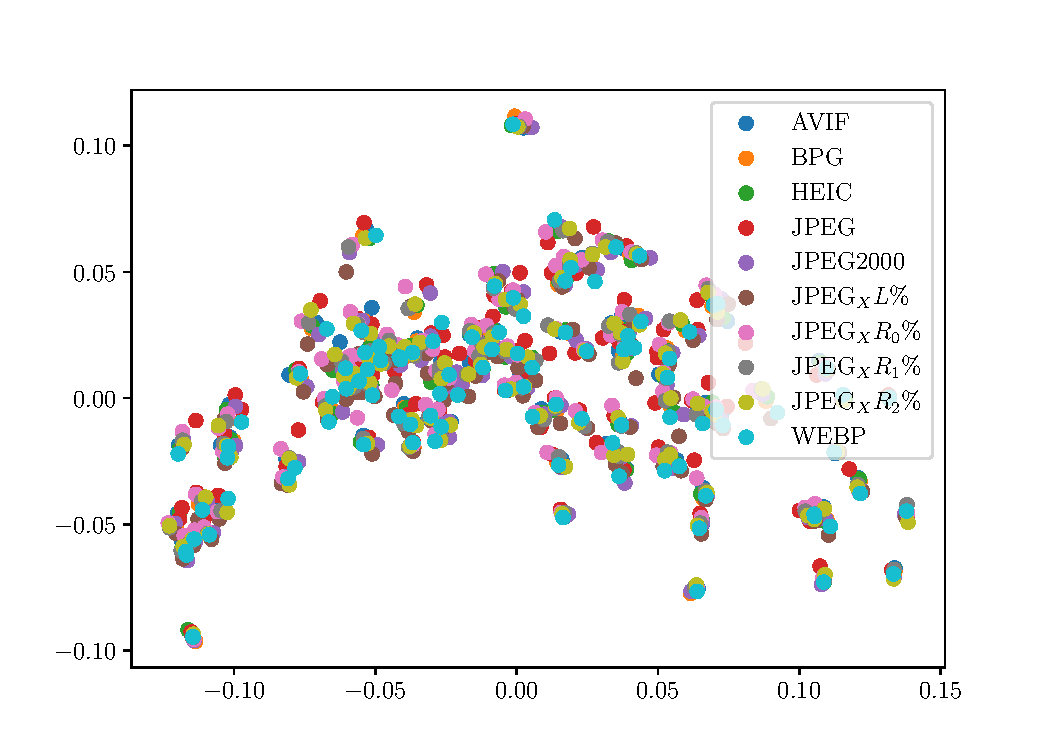
\includegraphics[width=\textwidth]{Plots/plot_scatter_without_transfer_10.pgf}
	\caption{10kB Compression: ResNet without transfer learning}
	\label{fig: no_transfer}
\end{figure}


\section{Performance}
For the classification each model was evaluated with each filesize. The result is represented in the figure \ref{fig: acc_comparison}.

\begin{figure}[h!]
	\centering
	\resizebox{\textwidth}{!}{%% Creator: Matplotlib, PGF backend
%%
%% To include the figure in your LaTeX document, write
%%   \input{<filename>.pgf}
%%
%% Make sure the required packages are loaded in your preamble
%%   \usepackage{pgf}
%%
%% Also ensure that all the required font packages are loaded; for instance,
%% the lmodern package is sometimes necessary when using math font.
%%   \usepackage{lmodern}
%%
%% Figures using additional raster images can only be included by \input if
%% they are in the same directory as the main LaTeX file. For loading figures
%% from other directories you can use the `import` package
%%   \usepackage{import}
%%
%% and then include the figures with
%%   \import{<path to file>}{<filename>.pgf}
%%
%% Matplotlib used the following preamble
%%   
%%   \makeatletter\@ifpackageloaded{underscore}{}{\usepackage[strings]{underscore}}\makeatother
%%
\begingroup%
\makeatletter%
\begin{pgfpicture}%
\pgfpathrectangle{\pgfpointorigin}{\pgfqpoint{9.000000in}{5.000000in}}%
\pgfusepath{use as bounding box, clip}%
\begin{pgfscope}%
\pgfsetbuttcap%
\pgfsetmiterjoin%
\definecolor{currentfill}{rgb}{1.000000,1.000000,1.000000}%
\pgfsetfillcolor{currentfill}%
\pgfsetlinewidth{0.000000pt}%
\definecolor{currentstroke}{rgb}{1.000000,1.000000,1.000000}%
\pgfsetstrokecolor{currentstroke}%
\pgfsetdash{}{0pt}%
\pgfpathmoveto{\pgfqpoint{0.000000in}{0.000000in}}%
\pgfpathlineto{\pgfqpoint{9.000000in}{0.000000in}}%
\pgfpathlineto{\pgfqpoint{9.000000in}{5.000000in}}%
\pgfpathlineto{\pgfqpoint{0.000000in}{5.000000in}}%
\pgfpathlineto{\pgfqpoint{0.000000in}{0.000000in}}%
\pgfpathclose%
\pgfusepath{fill}%
\end{pgfscope}%
\begin{pgfscope}%
\pgfsetbuttcap%
\pgfsetmiterjoin%
\definecolor{currentfill}{rgb}{1.000000,1.000000,1.000000}%
\pgfsetfillcolor{currentfill}%
\pgfsetlinewidth{0.000000pt}%
\definecolor{currentstroke}{rgb}{0.000000,0.000000,0.000000}%
\pgfsetstrokecolor{currentstroke}%
\pgfsetstrokeopacity{0.000000}%
\pgfsetdash{}{0pt}%
\pgfpathmoveto{\pgfqpoint{0.689449in}{0.629073in}}%
\pgfpathlineto{\pgfqpoint{6.363363in}{0.629073in}}%
\pgfpathlineto{\pgfqpoint{6.363363in}{4.820000in}}%
\pgfpathlineto{\pgfqpoint{0.689449in}{4.820000in}}%
\pgfpathlineto{\pgfqpoint{0.689449in}{0.629073in}}%
\pgfpathclose%
\pgfusepath{fill}%
\end{pgfscope}%
\begin{pgfscope}%
\pgfpathrectangle{\pgfqpoint{0.689449in}{0.629073in}}{\pgfqpoint{5.673914in}{4.190927in}}%
\pgfusepath{clip}%
\pgfsetrectcap%
\pgfsetroundjoin%
\pgfsetlinewidth{0.803000pt}%
\definecolor{currentstroke}{rgb}{0.690196,0.690196,0.690196}%
\pgfsetstrokecolor{currentstroke}%
\pgfsetdash{}{0pt}%
\pgfpathmoveto{\pgfqpoint{1.761792in}{0.629073in}}%
\pgfpathlineto{\pgfqpoint{1.761792in}{4.820000in}}%
\pgfusepath{stroke}%
\end{pgfscope}%
\begin{pgfscope}%
\pgfsetbuttcap%
\pgfsetroundjoin%
\definecolor{currentfill}{rgb}{0.000000,0.000000,0.000000}%
\pgfsetfillcolor{currentfill}%
\pgfsetlinewidth{0.803000pt}%
\definecolor{currentstroke}{rgb}{0.000000,0.000000,0.000000}%
\pgfsetstrokecolor{currentstroke}%
\pgfsetdash{}{0pt}%
\pgfsys@defobject{currentmarker}{\pgfqpoint{0.000000in}{-0.048611in}}{\pgfqpoint{0.000000in}{0.000000in}}{%
\pgfpathmoveto{\pgfqpoint{0.000000in}{0.000000in}}%
\pgfpathlineto{\pgfqpoint{0.000000in}{-0.048611in}}%
\pgfusepath{stroke,fill}%
}%
\begin{pgfscope}%
\pgfsys@transformshift{1.761792in}{0.629073in}%
\pgfsys@useobject{currentmarker}{}%
\end{pgfscope}%
\end{pgfscope}%
\begin{pgfscope}%
\definecolor{textcolor}{rgb}{0.000000,0.000000,0.000000}%
\pgfsetstrokecolor{textcolor}%
\pgfsetfillcolor{textcolor}%
\pgftext[x=1.761792in,y=0.531851in,,top]{\color{textcolor}\rmfamily\fontsize{12.000000}{14.400000}\selectfont \(\displaystyle {20}\)}%
\end{pgfscope}%
\begin{pgfscope}%
\pgfpathrectangle{\pgfqpoint{0.689449in}{0.629073in}}{\pgfqpoint{5.673914in}{4.190927in}}%
\pgfusepath{clip}%
\pgfsetrectcap%
\pgfsetroundjoin%
\pgfsetlinewidth{0.803000pt}%
\definecolor{currentstroke}{rgb}{0.690196,0.690196,0.690196}%
\pgfsetstrokecolor{currentstroke}%
\pgfsetdash{}{0pt}%
\pgfpathmoveto{\pgfqpoint{2.847708in}{0.629073in}}%
\pgfpathlineto{\pgfqpoint{2.847708in}{4.820000in}}%
\pgfusepath{stroke}%
\end{pgfscope}%
\begin{pgfscope}%
\pgfsetbuttcap%
\pgfsetroundjoin%
\definecolor{currentfill}{rgb}{0.000000,0.000000,0.000000}%
\pgfsetfillcolor{currentfill}%
\pgfsetlinewidth{0.803000pt}%
\definecolor{currentstroke}{rgb}{0.000000,0.000000,0.000000}%
\pgfsetstrokecolor{currentstroke}%
\pgfsetdash{}{0pt}%
\pgfsys@defobject{currentmarker}{\pgfqpoint{0.000000in}{-0.048611in}}{\pgfqpoint{0.000000in}{0.000000in}}{%
\pgfpathmoveto{\pgfqpoint{0.000000in}{0.000000in}}%
\pgfpathlineto{\pgfqpoint{0.000000in}{-0.048611in}}%
\pgfusepath{stroke,fill}%
}%
\begin{pgfscope}%
\pgfsys@transformshift{2.847708in}{0.629073in}%
\pgfsys@useobject{currentmarker}{}%
\end{pgfscope}%
\end{pgfscope}%
\begin{pgfscope}%
\definecolor{textcolor}{rgb}{0.000000,0.000000,0.000000}%
\pgfsetstrokecolor{textcolor}%
\pgfsetfillcolor{textcolor}%
\pgftext[x=2.847708in,y=0.531851in,,top]{\color{textcolor}\rmfamily\fontsize{12.000000}{14.400000}\selectfont \(\displaystyle {40}\)}%
\end{pgfscope}%
\begin{pgfscope}%
\pgfpathrectangle{\pgfqpoint{0.689449in}{0.629073in}}{\pgfqpoint{5.673914in}{4.190927in}}%
\pgfusepath{clip}%
\pgfsetrectcap%
\pgfsetroundjoin%
\pgfsetlinewidth{0.803000pt}%
\definecolor{currentstroke}{rgb}{0.690196,0.690196,0.690196}%
\pgfsetstrokecolor{currentstroke}%
\pgfsetdash{}{0pt}%
\pgfpathmoveto{\pgfqpoint{3.933625in}{0.629073in}}%
\pgfpathlineto{\pgfqpoint{3.933625in}{4.820000in}}%
\pgfusepath{stroke}%
\end{pgfscope}%
\begin{pgfscope}%
\pgfsetbuttcap%
\pgfsetroundjoin%
\definecolor{currentfill}{rgb}{0.000000,0.000000,0.000000}%
\pgfsetfillcolor{currentfill}%
\pgfsetlinewidth{0.803000pt}%
\definecolor{currentstroke}{rgb}{0.000000,0.000000,0.000000}%
\pgfsetstrokecolor{currentstroke}%
\pgfsetdash{}{0pt}%
\pgfsys@defobject{currentmarker}{\pgfqpoint{0.000000in}{-0.048611in}}{\pgfqpoint{0.000000in}{0.000000in}}{%
\pgfpathmoveto{\pgfqpoint{0.000000in}{0.000000in}}%
\pgfpathlineto{\pgfqpoint{0.000000in}{-0.048611in}}%
\pgfusepath{stroke,fill}%
}%
\begin{pgfscope}%
\pgfsys@transformshift{3.933625in}{0.629073in}%
\pgfsys@useobject{currentmarker}{}%
\end{pgfscope}%
\end{pgfscope}%
\begin{pgfscope}%
\definecolor{textcolor}{rgb}{0.000000,0.000000,0.000000}%
\pgfsetstrokecolor{textcolor}%
\pgfsetfillcolor{textcolor}%
\pgftext[x=3.933625in,y=0.531851in,,top]{\color{textcolor}\rmfamily\fontsize{12.000000}{14.400000}\selectfont \(\displaystyle {60}\)}%
\end{pgfscope}%
\begin{pgfscope}%
\pgfpathrectangle{\pgfqpoint{0.689449in}{0.629073in}}{\pgfqpoint{5.673914in}{4.190927in}}%
\pgfusepath{clip}%
\pgfsetrectcap%
\pgfsetroundjoin%
\pgfsetlinewidth{0.803000pt}%
\definecolor{currentstroke}{rgb}{0.690196,0.690196,0.690196}%
\pgfsetstrokecolor{currentstroke}%
\pgfsetdash{}{0pt}%
\pgfpathmoveto{\pgfqpoint{5.019542in}{0.629073in}}%
\pgfpathlineto{\pgfqpoint{5.019542in}{4.820000in}}%
\pgfusepath{stroke}%
\end{pgfscope}%
\begin{pgfscope}%
\pgfsetbuttcap%
\pgfsetroundjoin%
\definecolor{currentfill}{rgb}{0.000000,0.000000,0.000000}%
\pgfsetfillcolor{currentfill}%
\pgfsetlinewidth{0.803000pt}%
\definecolor{currentstroke}{rgb}{0.000000,0.000000,0.000000}%
\pgfsetstrokecolor{currentstroke}%
\pgfsetdash{}{0pt}%
\pgfsys@defobject{currentmarker}{\pgfqpoint{0.000000in}{-0.048611in}}{\pgfqpoint{0.000000in}{0.000000in}}{%
\pgfpathmoveto{\pgfqpoint{0.000000in}{0.000000in}}%
\pgfpathlineto{\pgfqpoint{0.000000in}{-0.048611in}}%
\pgfusepath{stroke,fill}%
}%
\begin{pgfscope}%
\pgfsys@transformshift{5.019542in}{0.629073in}%
\pgfsys@useobject{currentmarker}{}%
\end{pgfscope}%
\end{pgfscope}%
\begin{pgfscope}%
\definecolor{textcolor}{rgb}{0.000000,0.000000,0.000000}%
\pgfsetstrokecolor{textcolor}%
\pgfsetfillcolor{textcolor}%
\pgftext[x=5.019542in,y=0.531851in,,top]{\color{textcolor}\rmfamily\fontsize{12.000000}{14.400000}\selectfont \(\displaystyle {80}\)}%
\end{pgfscope}%
\begin{pgfscope}%
\pgfpathrectangle{\pgfqpoint{0.689449in}{0.629073in}}{\pgfqpoint{5.673914in}{4.190927in}}%
\pgfusepath{clip}%
\pgfsetrectcap%
\pgfsetroundjoin%
\pgfsetlinewidth{0.803000pt}%
\definecolor{currentstroke}{rgb}{0.690196,0.690196,0.690196}%
\pgfsetstrokecolor{currentstroke}%
\pgfsetdash{}{0pt}%
\pgfpathmoveto{\pgfqpoint{6.105458in}{0.629073in}}%
\pgfpathlineto{\pgfqpoint{6.105458in}{4.820000in}}%
\pgfusepath{stroke}%
\end{pgfscope}%
\begin{pgfscope}%
\pgfsetbuttcap%
\pgfsetroundjoin%
\definecolor{currentfill}{rgb}{0.000000,0.000000,0.000000}%
\pgfsetfillcolor{currentfill}%
\pgfsetlinewidth{0.803000pt}%
\definecolor{currentstroke}{rgb}{0.000000,0.000000,0.000000}%
\pgfsetstrokecolor{currentstroke}%
\pgfsetdash{}{0pt}%
\pgfsys@defobject{currentmarker}{\pgfqpoint{0.000000in}{-0.048611in}}{\pgfqpoint{0.000000in}{0.000000in}}{%
\pgfpathmoveto{\pgfqpoint{0.000000in}{0.000000in}}%
\pgfpathlineto{\pgfqpoint{0.000000in}{-0.048611in}}%
\pgfusepath{stroke,fill}%
}%
\begin{pgfscope}%
\pgfsys@transformshift{6.105458in}{0.629073in}%
\pgfsys@useobject{currentmarker}{}%
\end{pgfscope}%
\end{pgfscope}%
\begin{pgfscope}%
\definecolor{textcolor}{rgb}{0.000000,0.000000,0.000000}%
\pgfsetstrokecolor{textcolor}%
\pgfsetfillcolor{textcolor}%
\pgftext[x=6.105458in,y=0.531851in,,top]{\color{textcolor}\rmfamily\fontsize{12.000000}{14.400000}\selectfont \(\displaystyle {100}\)}%
\end{pgfscope}%
\begin{pgfscope}%
\definecolor{textcolor}{rgb}{0.000000,0.000000,0.000000}%
\pgfsetstrokecolor{textcolor}%
\pgfsetfillcolor{textcolor}%
\pgftext[x=3.526406in,y=0.328147in,,top]{\color{textcolor}\rmfamily\fontsize{12.000000}{14.400000}\selectfont Test Filesize}%
\end{pgfscope}%
\begin{pgfscope}%
\pgfpathrectangle{\pgfqpoint{0.689449in}{0.629073in}}{\pgfqpoint{5.673914in}{4.190927in}}%
\pgfusepath{clip}%
\pgfsetrectcap%
\pgfsetroundjoin%
\pgfsetlinewidth{0.803000pt}%
\definecolor{currentstroke}{rgb}{0.690196,0.690196,0.690196}%
\pgfsetstrokecolor{currentstroke}%
\pgfsetdash{}{0pt}%
\pgfpathmoveto{\pgfqpoint{0.689449in}{1.136547in}}%
\pgfpathlineto{\pgfqpoint{6.363363in}{1.136547in}}%
\pgfusepath{stroke}%
\end{pgfscope}%
\begin{pgfscope}%
\pgfsetbuttcap%
\pgfsetroundjoin%
\definecolor{currentfill}{rgb}{0.000000,0.000000,0.000000}%
\pgfsetfillcolor{currentfill}%
\pgfsetlinewidth{0.803000pt}%
\definecolor{currentstroke}{rgb}{0.000000,0.000000,0.000000}%
\pgfsetstrokecolor{currentstroke}%
\pgfsetdash{}{0pt}%
\pgfsys@defobject{currentmarker}{\pgfqpoint{-0.048611in}{0.000000in}}{\pgfqpoint{-0.000000in}{0.000000in}}{%
\pgfpathmoveto{\pgfqpoint{-0.000000in}{0.000000in}}%
\pgfpathlineto{\pgfqpoint{-0.048611in}{0.000000in}}%
\pgfusepath{stroke,fill}%
}%
\begin{pgfscope}%
\pgfsys@transformshift{0.689449in}{1.136547in}%
\pgfsys@useobject{currentmarker}{}%
\end{pgfscope}%
\end{pgfscope}%
\begin{pgfscope}%
\definecolor{textcolor}{rgb}{0.000000,0.000000,0.000000}%
\pgfsetstrokecolor{textcolor}%
\pgfsetfillcolor{textcolor}%
\pgftext[x=0.383703in, y=1.078677in, left, base]{\color{textcolor}\rmfamily\fontsize{12.000000}{14.400000}\selectfont \(\displaystyle {0.2}\)}%
\end{pgfscope}%
\begin{pgfscope}%
\pgfpathrectangle{\pgfqpoint{0.689449in}{0.629073in}}{\pgfqpoint{5.673914in}{4.190927in}}%
\pgfusepath{clip}%
\pgfsetrectcap%
\pgfsetroundjoin%
\pgfsetlinewidth{0.803000pt}%
\definecolor{currentstroke}{rgb}{0.690196,0.690196,0.690196}%
\pgfsetstrokecolor{currentstroke}%
\pgfsetdash{}{0pt}%
\pgfpathmoveto{\pgfqpoint{0.689449in}{2.021961in}}%
\pgfpathlineto{\pgfqpoint{6.363363in}{2.021961in}}%
\pgfusepath{stroke}%
\end{pgfscope}%
\begin{pgfscope}%
\pgfsetbuttcap%
\pgfsetroundjoin%
\definecolor{currentfill}{rgb}{0.000000,0.000000,0.000000}%
\pgfsetfillcolor{currentfill}%
\pgfsetlinewidth{0.803000pt}%
\definecolor{currentstroke}{rgb}{0.000000,0.000000,0.000000}%
\pgfsetstrokecolor{currentstroke}%
\pgfsetdash{}{0pt}%
\pgfsys@defobject{currentmarker}{\pgfqpoint{-0.048611in}{0.000000in}}{\pgfqpoint{-0.000000in}{0.000000in}}{%
\pgfpathmoveto{\pgfqpoint{-0.000000in}{0.000000in}}%
\pgfpathlineto{\pgfqpoint{-0.048611in}{0.000000in}}%
\pgfusepath{stroke,fill}%
}%
\begin{pgfscope}%
\pgfsys@transformshift{0.689449in}{2.021961in}%
\pgfsys@useobject{currentmarker}{}%
\end{pgfscope}%
\end{pgfscope}%
\begin{pgfscope}%
\definecolor{textcolor}{rgb}{0.000000,0.000000,0.000000}%
\pgfsetstrokecolor{textcolor}%
\pgfsetfillcolor{textcolor}%
\pgftext[x=0.383703in, y=1.964091in, left, base]{\color{textcolor}\rmfamily\fontsize{12.000000}{14.400000}\selectfont \(\displaystyle {0.4}\)}%
\end{pgfscope}%
\begin{pgfscope}%
\pgfpathrectangle{\pgfqpoint{0.689449in}{0.629073in}}{\pgfqpoint{5.673914in}{4.190927in}}%
\pgfusepath{clip}%
\pgfsetrectcap%
\pgfsetroundjoin%
\pgfsetlinewidth{0.803000pt}%
\definecolor{currentstroke}{rgb}{0.690196,0.690196,0.690196}%
\pgfsetstrokecolor{currentstroke}%
\pgfsetdash{}{0pt}%
\pgfpathmoveto{\pgfqpoint{0.689449in}{2.907374in}}%
\pgfpathlineto{\pgfqpoint{6.363363in}{2.907374in}}%
\pgfusepath{stroke}%
\end{pgfscope}%
\begin{pgfscope}%
\pgfsetbuttcap%
\pgfsetroundjoin%
\definecolor{currentfill}{rgb}{0.000000,0.000000,0.000000}%
\pgfsetfillcolor{currentfill}%
\pgfsetlinewidth{0.803000pt}%
\definecolor{currentstroke}{rgb}{0.000000,0.000000,0.000000}%
\pgfsetstrokecolor{currentstroke}%
\pgfsetdash{}{0pt}%
\pgfsys@defobject{currentmarker}{\pgfqpoint{-0.048611in}{0.000000in}}{\pgfqpoint{-0.000000in}{0.000000in}}{%
\pgfpathmoveto{\pgfqpoint{-0.000000in}{0.000000in}}%
\pgfpathlineto{\pgfqpoint{-0.048611in}{0.000000in}}%
\pgfusepath{stroke,fill}%
}%
\begin{pgfscope}%
\pgfsys@transformshift{0.689449in}{2.907374in}%
\pgfsys@useobject{currentmarker}{}%
\end{pgfscope}%
\end{pgfscope}%
\begin{pgfscope}%
\definecolor{textcolor}{rgb}{0.000000,0.000000,0.000000}%
\pgfsetstrokecolor{textcolor}%
\pgfsetfillcolor{textcolor}%
\pgftext[x=0.383703in, y=2.849504in, left, base]{\color{textcolor}\rmfamily\fontsize{12.000000}{14.400000}\selectfont \(\displaystyle {0.6}\)}%
\end{pgfscope}%
\begin{pgfscope}%
\pgfpathrectangle{\pgfqpoint{0.689449in}{0.629073in}}{\pgfqpoint{5.673914in}{4.190927in}}%
\pgfusepath{clip}%
\pgfsetrectcap%
\pgfsetroundjoin%
\pgfsetlinewidth{0.803000pt}%
\definecolor{currentstroke}{rgb}{0.690196,0.690196,0.690196}%
\pgfsetstrokecolor{currentstroke}%
\pgfsetdash{}{0pt}%
\pgfpathmoveto{\pgfqpoint{0.689449in}{3.792788in}}%
\pgfpathlineto{\pgfqpoint{6.363363in}{3.792788in}}%
\pgfusepath{stroke}%
\end{pgfscope}%
\begin{pgfscope}%
\pgfsetbuttcap%
\pgfsetroundjoin%
\definecolor{currentfill}{rgb}{0.000000,0.000000,0.000000}%
\pgfsetfillcolor{currentfill}%
\pgfsetlinewidth{0.803000pt}%
\definecolor{currentstroke}{rgb}{0.000000,0.000000,0.000000}%
\pgfsetstrokecolor{currentstroke}%
\pgfsetdash{}{0pt}%
\pgfsys@defobject{currentmarker}{\pgfqpoint{-0.048611in}{0.000000in}}{\pgfqpoint{-0.000000in}{0.000000in}}{%
\pgfpathmoveto{\pgfqpoint{-0.000000in}{0.000000in}}%
\pgfpathlineto{\pgfqpoint{-0.048611in}{0.000000in}}%
\pgfusepath{stroke,fill}%
}%
\begin{pgfscope}%
\pgfsys@transformshift{0.689449in}{3.792788in}%
\pgfsys@useobject{currentmarker}{}%
\end{pgfscope}%
\end{pgfscope}%
\begin{pgfscope}%
\definecolor{textcolor}{rgb}{0.000000,0.000000,0.000000}%
\pgfsetstrokecolor{textcolor}%
\pgfsetfillcolor{textcolor}%
\pgftext[x=0.383703in, y=3.734917in, left, base]{\color{textcolor}\rmfamily\fontsize{12.000000}{14.400000}\selectfont \(\displaystyle {0.8}\)}%
\end{pgfscope}%
\begin{pgfscope}%
\pgfpathrectangle{\pgfqpoint{0.689449in}{0.629073in}}{\pgfqpoint{5.673914in}{4.190927in}}%
\pgfusepath{clip}%
\pgfsetrectcap%
\pgfsetroundjoin%
\pgfsetlinewidth{0.803000pt}%
\definecolor{currentstroke}{rgb}{0.690196,0.690196,0.690196}%
\pgfsetstrokecolor{currentstroke}%
\pgfsetdash{}{0pt}%
\pgfpathmoveto{\pgfqpoint{0.689449in}{4.678201in}}%
\pgfpathlineto{\pgfqpoint{6.363363in}{4.678201in}}%
\pgfusepath{stroke}%
\end{pgfscope}%
\begin{pgfscope}%
\pgfsetbuttcap%
\pgfsetroundjoin%
\definecolor{currentfill}{rgb}{0.000000,0.000000,0.000000}%
\pgfsetfillcolor{currentfill}%
\pgfsetlinewidth{0.803000pt}%
\definecolor{currentstroke}{rgb}{0.000000,0.000000,0.000000}%
\pgfsetstrokecolor{currentstroke}%
\pgfsetdash{}{0pt}%
\pgfsys@defobject{currentmarker}{\pgfqpoint{-0.048611in}{0.000000in}}{\pgfqpoint{-0.000000in}{0.000000in}}{%
\pgfpathmoveto{\pgfqpoint{-0.000000in}{0.000000in}}%
\pgfpathlineto{\pgfqpoint{-0.048611in}{0.000000in}}%
\pgfusepath{stroke,fill}%
}%
\begin{pgfscope}%
\pgfsys@transformshift{0.689449in}{4.678201in}%
\pgfsys@useobject{currentmarker}{}%
\end{pgfscope}%
\end{pgfscope}%
\begin{pgfscope}%
\definecolor{textcolor}{rgb}{0.000000,0.000000,0.000000}%
\pgfsetstrokecolor{textcolor}%
\pgfsetfillcolor{textcolor}%
\pgftext[x=0.383703in, y=4.620331in, left, base]{\color{textcolor}\rmfamily\fontsize{12.000000}{14.400000}\selectfont \(\displaystyle {1.0}\)}%
\end{pgfscope}%
\begin{pgfscope}%
\definecolor{textcolor}{rgb}{0.000000,0.000000,0.000000}%
\pgfsetstrokecolor{textcolor}%
\pgfsetfillcolor{textcolor}%
\pgftext[x=0.328148in,y=2.724536in,,bottom,rotate=90.000000]{\color{textcolor}\rmfamily\fontsize{12.000000}{14.400000}\selectfont Accuracy}%
\end{pgfscope}%
\begin{pgfscope}%
\pgfpathrectangle{\pgfqpoint{0.689449in}{0.629073in}}{\pgfqpoint{5.673914in}{4.190927in}}%
\pgfusepath{clip}%
\pgfsetrectcap%
\pgfsetroundjoin%
\pgfsetlinewidth{1.505625pt}%
\definecolor{currentstroke}{rgb}{0.121569,0.466667,0.705882}%
\pgfsetstrokecolor{currentstroke}%
\pgfsetdash{}{0pt}%
\pgfpathmoveto{\pgfqpoint{0.947354in}{4.518827in}}%
\pgfpathlineto{\pgfqpoint{1.218834in}{4.554243in}}%
\pgfpathlineto{\pgfqpoint{1.598904in}{4.505545in}}%
\pgfpathlineto{\pgfqpoint{2.033271in}{4.439139in}}%
\pgfpathlineto{\pgfqpoint{2.413342in}{4.394869in}}%
\pgfpathlineto{\pgfqpoint{2.847708in}{4.315182in}}%
\pgfpathlineto{\pgfqpoint{3.390667in}{4.053985in}}%
\pgfpathlineto{\pgfqpoint{3.933625in}{3.713100in}}%
\pgfpathlineto{\pgfqpoint{4.748062in}{3.035759in}}%
\pgfpathlineto{\pgfqpoint{6.105458in}{2.021961in}}%
\pgfusepath{stroke}%
\end{pgfscope}%
\begin{pgfscope}%
\pgfpathrectangle{\pgfqpoint{0.689449in}{0.629073in}}{\pgfqpoint{5.673914in}{4.190927in}}%
\pgfusepath{clip}%
\pgfsetrectcap%
\pgfsetroundjoin%
\pgfsetlinewidth{1.505625pt}%
\definecolor{currentstroke}{rgb}{0.200000,0.627451,0.172549}%
\pgfsetstrokecolor{currentstroke}%
\pgfsetdash{}{0pt}%
\pgfpathmoveto{\pgfqpoint{0.947354in}{2.557636in}}%
\pgfpathlineto{\pgfqpoint{1.218834in}{3.000343in}}%
\pgfpathlineto{\pgfqpoint{1.598904in}{3.168571in}}%
\pgfpathlineto{\pgfqpoint{2.033271in}{3.009197in}}%
\pgfpathlineto{\pgfqpoint{2.413342in}{2.712583in}}%
\pgfpathlineto{\pgfqpoint{2.847708in}{2.314147in}}%
\pgfpathlineto{\pgfqpoint{3.390667in}{1.681077in}}%
\pgfpathlineto{\pgfqpoint{3.933625in}{1.353474in}}%
\pgfpathlineto{\pgfqpoint{4.748062in}{1.078996in}}%
\pgfpathlineto{\pgfqpoint{6.105458in}{0.897486in}}%
\pgfusepath{stroke}%
\end{pgfscope}%
\begin{pgfscope}%
\pgfpathrectangle{\pgfqpoint{0.689449in}{0.629073in}}{\pgfqpoint{5.673914in}{4.190927in}}%
\pgfusepath{clip}%
\pgfsetrectcap%
\pgfsetroundjoin%
\pgfsetlinewidth{1.505625pt}%
\definecolor{currentstroke}{rgb}{0.192157,0.509804,0.741176}%
\pgfsetstrokecolor{currentstroke}%
\pgfsetdash{}{0pt}%
\pgfpathmoveto{\pgfqpoint{0.947354in}{4.598514in}}%
\pgfpathlineto{\pgfqpoint{1.218834in}{4.598514in}}%
\pgfpathlineto{\pgfqpoint{1.598904in}{4.629503in}}%
\pgfpathlineto{\pgfqpoint{2.033271in}{4.602941in}}%
\pgfpathlineto{\pgfqpoint{2.413342in}{4.594087in}}%
\pgfpathlineto{\pgfqpoint{2.847708in}{4.554243in}}%
\pgfpathlineto{\pgfqpoint{3.390667in}{4.514400in}}%
\pgfpathlineto{\pgfqpoint{3.933625in}{4.425858in}}%
\pgfpathlineto{\pgfqpoint{4.748062in}{4.279765in}}%
\pgfpathlineto{\pgfqpoint{6.105458in}{3.969870in}}%
\pgfusepath{stroke}%
\end{pgfscope}%
\begin{pgfscope}%
\pgfpathrectangle{\pgfqpoint{0.689449in}{0.629073in}}{\pgfqpoint{5.673914in}{4.190927in}}%
\pgfusepath{clip}%
\pgfsetrectcap%
\pgfsetroundjoin%
\pgfsetlinewidth{1.505625pt}%
\definecolor{currentstroke}{rgb}{0.890196,0.101961,0.109804}%
\pgfsetstrokecolor{currentstroke}%
\pgfsetdash{}{0pt}%
\pgfpathmoveto{\pgfqpoint{0.947354in}{4.541875in}}%
\pgfpathlineto{\pgfqpoint{1.218834in}{4.365650in}}%
\pgfpathlineto{\pgfqpoint{1.598904in}{3.643153in}}%
\pgfpathlineto{\pgfqpoint{2.033271in}{2.788729in}}%
\pgfpathlineto{\pgfqpoint{2.413342in}{2.092794in}}%
\pgfpathlineto{\pgfqpoint{2.847708in}{1.648316in}}%
\pgfpathlineto{\pgfqpoint{3.390667in}{1.310088in}}%
\pgfpathlineto{\pgfqpoint{3.933625in}{1.043579in}}%
\pgfpathlineto{\pgfqpoint{4.748062in}{0.924934in}}%
\pgfpathlineto{\pgfqpoint{6.105458in}{0.819569in}}%
\pgfusepath{stroke}%
\end{pgfscope}%
\begin{pgfscope}%
\pgfpathrectangle{\pgfqpoint{0.689449in}{0.629073in}}{\pgfqpoint{5.673914in}{4.190927in}}%
\pgfusepath{clip}%
\pgfsetrectcap%
\pgfsetroundjoin%
\pgfsetlinewidth{1.505625pt}%
\definecolor{currentstroke}{rgb}{1.000000,0.498039,0.000000}%
\pgfsetstrokecolor{currentstroke}%
\pgfsetdash{}{0pt}%
\pgfpathmoveto{\pgfqpoint{0.947354in}{4.514432in}}%
\pgfpathlineto{\pgfqpoint{1.218834in}{4.552472in}}%
\pgfpathlineto{\pgfqpoint{1.598904in}{4.423202in}}%
\pgfpathlineto{\pgfqpoint{2.033271in}{3.961016in}}%
\pgfpathlineto{\pgfqpoint{2.413342in}{3.431539in}}%
\pgfpathlineto{\pgfqpoint{2.847708in}{2.833885in}}%
\pgfpathlineto{\pgfqpoint{3.390667in}{2.200814in}}%
\pgfpathlineto{\pgfqpoint{3.933625in}{1.789097in}}%
\pgfpathlineto{\pgfqpoint{4.748062in}{1.365870in}}%
\pgfpathlineto{\pgfqpoint{6.105458in}{1.099360in}}%
\pgfusepath{stroke}%
\end{pgfscope}%
\begin{pgfscope}%
\pgfpathrectangle{\pgfqpoint{0.689449in}{0.629073in}}{\pgfqpoint{5.673914in}{4.190927in}}%
\pgfusepath{clip}%
\pgfsetrectcap%
\pgfsetroundjoin%
\pgfsetlinewidth{1.505625pt}%
\definecolor{currentstroke}{rgb}{0.415686,0.239216,0.603922}%
\pgfsetstrokecolor{currentstroke}%
\pgfsetdash{}{0pt}%
\pgfpathmoveto{\pgfqpoint{0.947354in}{4.253288in}}%
\pgfpathlineto{\pgfqpoint{1.218834in}{4.524139in}}%
\pgfpathlineto{\pgfqpoint{1.598904in}{4.494920in}}%
\pgfpathlineto{\pgfqpoint{2.033271in}{4.355025in}}%
\pgfpathlineto{\pgfqpoint{2.413342in}{4.206276in}}%
\pgfpathlineto{\pgfqpoint{2.847708in}{3.923829in}}%
\pgfpathlineto{\pgfqpoint{3.390667in}{3.424456in}}%
\pgfpathlineto{\pgfqpoint{3.933625in}{2.835656in}}%
\pgfpathlineto{\pgfqpoint{4.748062in}{2.117586in}}%
\pgfpathlineto{\pgfqpoint{6.105458in}{1.412796in}}%
\pgfusepath{stroke}%
\end{pgfscope}%
\begin{pgfscope}%
\pgfpathrectangle{\pgfqpoint{0.689449in}{0.629073in}}{\pgfqpoint{5.673914in}{4.190927in}}%
\pgfusepath{clip}%
\pgfsetrectcap%
\pgfsetroundjoin%
\pgfsetlinewidth{1.505625pt}%
\definecolor{currentstroke}{rgb}{0.650980,0.462745,0.113725}%
\pgfsetstrokecolor{currentstroke}%
\pgfsetdash{}{0pt}%
\pgfpathmoveto{\pgfqpoint{0.947354in}{3.980635in}}%
\pgfpathlineto{\pgfqpoint{1.218834in}{4.470129in}}%
\pgfpathlineto{\pgfqpoint{1.598904in}{4.528566in}}%
\pgfpathlineto{\pgfqpoint{2.033271in}{4.514400in}}%
\pgfpathlineto{\pgfqpoint{2.413342in}{4.464816in}}%
\pgfpathlineto{\pgfqpoint{2.847708in}{4.350598in}}%
\pgfpathlineto{\pgfqpoint{3.390667in}{4.119505in}}%
\pgfpathlineto{\pgfqpoint{3.933625in}{3.828204in}}%
\pgfpathlineto{\pgfqpoint{4.748062in}{3.167686in}}%
\pgfpathlineto{\pgfqpoint{6.105458in}{2.052950in}}%
\pgfusepath{stroke}%
\end{pgfscope}%
\begin{pgfscope}%
\pgfpathrectangle{\pgfqpoint{0.689449in}{0.629073in}}{\pgfqpoint{5.673914in}{4.190927in}}%
\pgfusepath{clip}%
\pgfsetrectcap%
\pgfsetroundjoin%
\pgfsetlinewidth{1.505625pt}%
\definecolor{currentstroke}{rgb}{0.941176,0.007843,0.498039}%
\pgfsetstrokecolor{currentstroke}%
\pgfsetdash{}{0pt}%
\pgfpathmoveto{\pgfqpoint{0.947354in}{3.923980in}}%
\pgfpathlineto{\pgfqpoint{1.218834in}{4.383358in}}%
\pgfpathlineto{\pgfqpoint{1.598904in}{4.476327in}}%
\pgfpathlineto{\pgfqpoint{2.033271in}{4.478983in}}%
\pgfpathlineto{\pgfqpoint{2.413342in}{4.433827in}}%
\pgfpathlineto{\pgfqpoint{2.847708in}{4.360338in}}%
\pgfpathlineto{\pgfqpoint{3.390667in}{4.197422in}}%
\pgfpathlineto{\pgfqpoint{3.933625in}{3.960131in}}%
\pgfpathlineto{\pgfqpoint{4.748062in}{3.471383in}}%
\pgfpathlineto{\pgfqpoint{6.105458in}{2.570917in}}%
\pgfusepath{stroke}%
\end{pgfscope}%
\begin{pgfscope}%
\pgfpathrectangle{\pgfqpoint{0.689449in}{0.629073in}}{\pgfqpoint{5.673914in}{4.190927in}}%
\pgfusepath{clip}%
\pgfsetrectcap%
\pgfsetroundjoin%
\pgfsetlinewidth{1.505625pt}%
\definecolor{currentstroke}{rgb}{0.400000,0.400000,0.400000}%
\pgfsetstrokecolor{currentstroke}%
\pgfsetdash{}{0pt}%
\pgfpathmoveto{\pgfqpoint{0.947354in}{3.493755in}}%
\pgfpathlineto{\pgfqpoint{1.218834in}{4.238151in}}%
\pgfpathlineto{\pgfqpoint{1.598904in}{4.403723in}}%
\pgfpathlineto{\pgfqpoint{2.033271in}{4.475441in}}%
\pgfpathlineto{\pgfqpoint{2.413342in}{4.488723in}}%
\pgfpathlineto{\pgfqpoint{2.847708in}{4.454191in}}%
\pgfpathlineto{\pgfqpoint{3.390667in}{4.385129in}}%
\pgfpathlineto{\pgfqpoint{3.933625in}{4.265598in}}%
\pgfpathlineto{\pgfqpoint{4.748062in}{3.942423in}}%
\pgfpathlineto{\pgfqpoint{6.105458in}{3.007426in}}%
\pgfusepath{stroke}%
\end{pgfscope}%
\begin{pgfscope}%
\pgfpathrectangle{\pgfqpoint{0.689449in}{0.629073in}}{\pgfqpoint{5.673914in}{4.190927in}}%
\pgfusepath{clip}%
\pgfsetrectcap%
\pgfsetroundjoin%
\pgfsetlinewidth{1.505625pt}%
\definecolor{currentstroke}{rgb}{0.650980,0.847059,0.329412}%
\pgfsetstrokecolor{currentstroke}%
\pgfsetdash{}{0pt}%
\pgfpathmoveto{\pgfqpoint{0.947354in}{2.714747in}}%
\pgfpathlineto{\pgfqpoint{1.218834in}{3.480237in}}%
\pgfpathlineto{\pgfqpoint{1.598904in}{3.953933in}}%
\pgfpathlineto{\pgfqpoint{2.033271in}{4.162890in}}%
\pgfpathlineto{\pgfqpoint{2.413342in}{4.227526in}}%
\pgfpathlineto{\pgfqpoint{2.847708in}{4.283307in}}%
\pgfpathlineto{\pgfqpoint{3.390667in}{4.232838in}}%
\pgfpathlineto{\pgfqpoint{3.933625in}{4.061953in}}%
\pgfpathlineto{\pgfqpoint{4.748062in}{3.672371in}}%
\pgfpathlineto{\pgfqpoint{6.105458in}{2.590396in}}%
\pgfusepath{stroke}%
\end{pgfscope}%
\begin{pgfscope}%
\pgfpathrectangle{\pgfqpoint{0.689449in}{0.629073in}}{\pgfqpoint{5.673914in}{4.190927in}}%
\pgfusepath{clip}%
\pgfsetrectcap%
\pgfsetroundjoin%
\pgfsetlinewidth{1.505625pt}%
\definecolor{currentstroke}{rgb}{0.090196,0.745098,0.811765}%
\pgfsetstrokecolor{currentstroke}%
\pgfsetdash{}{0pt}%
\pgfpathmoveto{\pgfqpoint{0.947354in}{2.339407in}}%
\pgfpathlineto{\pgfqpoint{1.218834in}{3.096853in}}%
\pgfpathlineto{\pgfqpoint{1.598904in}{3.636955in}}%
\pgfpathlineto{\pgfqpoint{2.033271in}{3.934454in}}%
\pgfpathlineto{\pgfqpoint{2.413342in}{4.094714in}}%
\pgfpathlineto{\pgfqpoint{2.847708in}{4.212474in}}%
\pgfpathlineto{\pgfqpoint{3.390667in}{4.169974in}}%
\pgfpathlineto{\pgfqpoint{3.933625in}{4.077005in}}%
\pgfpathlineto{\pgfqpoint{4.748062in}{3.805183in}}%
\pgfpathlineto{\pgfqpoint{6.105458in}{2.948989in}}%
\pgfusepath{stroke}%
\end{pgfscope}%
\begin{pgfscope}%
\pgfpathrectangle{\pgfqpoint{0.689449in}{0.629073in}}{\pgfqpoint{5.673914in}{4.190927in}}%
\pgfusepath{clip}%
\pgfsetrectcap%
\pgfsetroundjoin%
\pgfsetlinewidth{1.505625pt}%
\definecolor{currentstroke}{rgb}{0.870588,0.619608,0.839216}%
\pgfsetstrokecolor{currentstroke}%
\pgfsetdash{}{0pt}%
\pgfpathmoveto{\pgfqpoint{0.947354in}{1.758692in}}%
\pgfpathlineto{\pgfqpoint{1.218834in}{2.868416in}}%
\pgfpathlineto{\pgfqpoint{1.598904in}{3.533362in}}%
\pgfpathlineto{\pgfqpoint{2.033271in}{3.899923in}}%
\pgfpathlineto{\pgfqpoint{2.413342in}{4.007943in}}%
\pgfpathlineto{\pgfqpoint{2.847708in}{4.157578in}}%
\pgfpathlineto{\pgfqpoint{3.390667in}{4.245234in}}%
\pgfpathlineto{\pgfqpoint{3.933625in}{4.218671in}}%
\pgfpathlineto{\pgfqpoint{4.748062in}{4.192109in}}%
\pgfpathlineto{\pgfqpoint{6.105458in}{3.728152in}}%
\pgfusepath{stroke}%
\end{pgfscope}%
\begin{pgfscope}%
\pgfpathrectangle{\pgfqpoint{0.689449in}{0.629073in}}{\pgfqpoint{5.673914in}{4.190927in}}%
\pgfusepath{clip}%
\pgfsetrectcap%
\pgfsetroundjoin%
\pgfsetlinewidth{1.505625pt}%
\definecolor{currentstroke}{rgb}{0.984314,0.705882,0.682353}%
\pgfsetstrokecolor{currentstroke}%
\pgfsetdash{}{0pt}%
\pgfpathmoveto{\pgfqpoint{0.947354in}{0.977028in}}%
\pgfpathlineto{\pgfqpoint{1.218834in}{1.792639in}}%
\pgfpathlineto{\pgfqpoint{1.598904in}{2.473522in}}%
\pgfpathlineto{\pgfqpoint{2.033271in}{2.926853in}}%
\pgfpathlineto{\pgfqpoint{2.413342in}{3.190707in}}%
\pgfpathlineto{\pgfqpoint{2.847708in}{3.430654in}}%
\pgfpathlineto{\pgfqpoint{3.390667in}{3.688309in}}%
\pgfpathlineto{\pgfqpoint{3.933625in}{3.887527in}}%
\pgfpathlineto{\pgfqpoint{4.748062in}{4.084089in}}%
\pgfpathlineto{\pgfqpoint{6.105458in}{3.988464in}}%
\pgfusepath{stroke}%
\end{pgfscope}%
\begin{pgfscope}%
\pgfsetrectcap%
\pgfsetmiterjoin%
\pgfsetlinewidth{0.803000pt}%
\definecolor{currentstroke}{rgb}{0.000000,0.000000,0.000000}%
\pgfsetstrokecolor{currentstroke}%
\pgfsetdash{}{0pt}%
\pgfpathmoveto{\pgfqpoint{0.689449in}{0.629073in}}%
\pgfpathlineto{\pgfqpoint{0.689449in}{4.820000in}}%
\pgfusepath{stroke}%
\end{pgfscope}%
\begin{pgfscope}%
\pgfsetrectcap%
\pgfsetmiterjoin%
\pgfsetlinewidth{0.803000pt}%
\definecolor{currentstroke}{rgb}{0.000000,0.000000,0.000000}%
\pgfsetstrokecolor{currentstroke}%
\pgfsetdash{}{0pt}%
\pgfpathmoveto{\pgfqpoint{6.363363in}{0.629073in}}%
\pgfpathlineto{\pgfqpoint{6.363363in}{4.820000in}}%
\pgfusepath{stroke}%
\end{pgfscope}%
\begin{pgfscope}%
\pgfsetrectcap%
\pgfsetmiterjoin%
\pgfsetlinewidth{0.803000pt}%
\definecolor{currentstroke}{rgb}{0.000000,0.000000,0.000000}%
\pgfsetstrokecolor{currentstroke}%
\pgfsetdash{}{0pt}%
\pgfpathmoveto{\pgfqpoint{0.689449in}{0.629073in}}%
\pgfpathlineto{\pgfqpoint{6.363363in}{0.629073in}}%
\pgfusepath{stroke}%
\end{pgfscope}%
\begin{pgfscope}%
\pgfsetrectcap%
\pgfsetmiterjoin%
\pgfsetlinewidth{0.803000pt}%
\definecolor{currentstroke}{rgb}{0.000000,0.000000,0.000000}%
\pgfsetstrokecolor{currentstroke}%
\pgfsetdash{}{0pt}%
\pgfpathmoveto{\pgfqpoint{0.689449in}{4.820000in}}%
\pgfpathlineto{\pgfqpoint{6.363363in}{4.820000in}}%
\pgfusepath{stroke}%
\end{pgfscope}%
\begin{pgfscope}%
\pgfsetbuttcap%
\pgfsetmiterjoin%
\definecolor{currentfill}{rgb}{1.000000,1.000000,1.000000}%
\pgfsetfillcolor{currentfill}%
\pgfsetfillopacity{0.800000}%
\pgfsetlinewidth{1.003750pt}%
\definecolor{currentstroke}{rgb}{0.800000,0.800000,0.800000}%
\pgfsetstrokecolor{currentstroke}%
\pgfsetstrokeopacity{0.800000}%
\pgfsetdash{}{0pt}%
\pgfpathmoveto{\pgfqpoint{6.480030in}{1.380189in}}%
\pgfpathlineto{\pgfqpoint{8.786667in}{1.380189in}}%
\pgfpathquadraticcurveto{\pgfqpoint{8.820000in}{1.380189in}}{\pgfqpoint{8.820000in}{1.413522in}}%
\pgfpathlineto{\pgfqpoint{8.820000in}{4.703333in}}%
\pgfpathquadraticcurveto{\pgfqpoint{8.820000in}{4.736667in}}{\pgfqpoint{8.786667in}{4.736667in}}%
\pgfpathlineto{\pgfqpoint{6.480030in}{4.736667in}}%
\pgfpathquadraticcurveto{\pgfqpoint{6.446697in}{4.736667in}}{\pgfqpoint{6.446697in}{4.703333in}}%
\pgfpathlineto{\pgfqpoint{6.446697in}{1.413522in}}%
\pgfpathquadraticcurveto{\pgfqpoint{6.446697in}{1.380189in}}{\pgfqpoint{6.480030in}{1.380189in}}%
\pgfpathlineto{\pgfqpoint{6.480030in}{1.380189in}}%
\pgfpathclose%
\pgfusepath{stroke,fill}%
\end{pgfscope}%
\begin{pgfscope}%
\definecolor{textcolor}{rgb}{0.000000,0.000000,0.000000}%
\pgfsetstrokecolor{textcolor}%
\pgfsetfillcolor{textcolor}%
\pgftext[x=6.528624in,y=4.545000in,left,base]{\color{textcolor}\rmfamily\fontsize{12.000000}{14.400000}\selectfont Trained file sizes (mean c-rate)}%
\end{pgfscope}%
\begin{pgfscope}%
\pgfsetrectcap%
\pgfsetroundjoin%
\pgfsetlinewidth{1.505625pt}%
\definecolor{currentstroke}{rgb}{0.121569,0.466667,0.705882}%
\pgfsetstrokecolor{currentstroke}%
\pgfsetdash{}{0pt}%
\pgfpathmoveto{\pgfqpoint{6.513363in}{4.353333in}}%
\pgfpathlineto{\pgfqpoint{6.680030in}{4.353333in}}%
\pgfpathlineto{\pgfqpoint{6.846697in}{4.353333in}}%
\pgfusepath{stroke}%
\end{pgfscope}%
\begin{pgfscope}%
\definecolor{textcolor}{rgb}{0.000000,0.000000,0.000000}%
\pgfsetstrokecolor{textcolor}%
\pgfsetfillcolor{textcolor}%
\pgftext[x=6.980030in,y=4.295000in,left,base]{\color{textcolor}\rmfamily\fontsize{12.000000}{14.400000}\selectfont Mixed pre trained (5-32)}%
\end{pgfscope}%
\begin{pgfscope}%
\pgfsetrectcap%
\pgfsetroundjoin%
\pgfsetlinewidth{1.505625pt}%
\definecolor{currentstroke}{rgb}{0.200000,0.627451,0.172549}%
\pgfsetstrokecolor{currentstroke}%
\pgfsetdash{}{0pt}%
\pgfpathmoveto{\pgfqpoint{6.513363in}{4.103333in}}%
\pgfpathlineto{\pgfqpoint{6.680030in}{4.103333in}}%
\pgfpathlineto{\pgfqpoint{6.846697in}{4.103333in}}%
\pgfusepath{stroke}%
\end{pgfscope}%
\begin{pgfscope}%
\definecolor{textcolor}{rgb}{0.000000,0.000000,0.000000}%
\pgfsetstrokecolor{textcolor}%
\pgfsetfillcolor{textcolor}%
\pgftext[x=6.980030in,y=4.045000in,left,base]{\color{textcolor}\rmfamily\fontsize{12.000000}{14.400000}\selectfont Mixed self trained (5-32)}%
\end{pgfscope}%
\begin{pgfscope}%
\pgfsetrectcap%
\pgfsetroundjoin%
\pgfsetlinewidth{1.505625pt}%
\definecolor{currentstroke}{rgb}{0.192157,0.509804,0.741176}%
\pgfsetstrokecolor{currentstroke}%
\pgfsetdash{}{0pt}%
\pgfpathmoveto{\pgfqpoint{6.513363in}{3.861667in}}%
\pgfpathlineto{\pgfqpoint{6.680030in}{3.861667in}}%
\pgfpathlineto{\pgfqpoint{6.846697in}{3.861667in}}%
\pgfusepath{stroke}%
\end{pgfscope}%
\begin{pgfscope}%
\definecolor{textcolor}{rgb}{0.000000,0.000000,0.000000}%
\pgfsetstrokecolor{textcolor}%
\pgfsetfillcolor{textcolor}%
\pgftext[x=6.980030in,y=3.803333in,left,base]{\color{textcolor}\rmfamily\fontsize{12.000000}{14.400000}\selectfont All file sizes}%
\end{pgfscope}%
\begin{pgfscope}%
\pgfsetrectcap%
\pgfsetroundjoin%
\pgfsetlinewidth{1.505625pt}%
\definecolor{currentstroke}{rgb}{0.890196,0.101961,0.109804}%
\pgfsetstrokecolor{currentstroke}%
\pgfsetdash{}{0pt}%
\pgfpathmoveto{\pgfqpoint{6.513363in}{3.629260in}}%
\pgfpathlineto{\pgfqpoint{6.680030in}{3.629260in}}%
\pgfpathlineto{\pgfqpoint{6.846697in}{3.629260in}}%
\pgfusepath{stroke}%
\end{pgfscope}%
\begin{pgfscope}%
\definecolor{textcolor}{rgb}{0.000000,0.000000,0.000000}%
\pgfsetstrokecolor{textcolor}%
\pgfsetfillcolor{textcolor}%
\pgftext[x=6.980030in,y=3.570926in,left,base]{\color{textcolor}\rmfamily\fontsize{12.000000}{14.400000}\selectfont 5  c-rate: 94.00}%
\end{pgfscope}%
\begin{pgfscope}%
\pgfsetrectcap%
\pgfsetroundjoin%
\pgfsetlinewidth{1.505625pt}%
\definecolor{currentstroke}{rgb}{1.000000,0.498039,0.000000}%
\pgfsetstrokecolor{currentstroke}%
\pgfsetdash{}{0pt}%
\pgfpathmoveto{\pgfqpoint{6.513363in}{3.396853in}}%
\pgfpathlineto{\pgfqpoint{6.680030in}{3.396853in}}%
\pgfpathlineto{\pgfqpoint{6.846697in}{3.396853in}}%
\pgfusepath{stroke}%
\end{pgfscope}%
\begin{pgfscope}%
\definecolor{textcolor}{rgb}{0.000000,0.000000,0.000000}%
\pgfsetstrokecolor{textcolor}%
\pgfsetfillcolor{textcolor}%
\pgftext[x=6.980030in,y=3.338519in,left,base]{\color{textcolor}\rmfamily\fontsize{12.000000}{14.400000}\selectfont 10  c-rate: 47.00}%
\end{pgfscope}%
\begin{pgfscope}%
\pgfsetrectcap%
\pgfsetroundjoin%
\pgfsetlinewidth{1.505625pt}%
\definecolor{currentstroke}{rgb}{0.415686,0.239216,0.603922}%
\pgfsetstrokecolor{currentstroke}%
\pgfsetdash{}{0pt}%
\pgfpathmoveto{\pgfqpoint{6.513363in}{3.164445in}}%
\pgfpathlineto{\pgfqpoint{6.680030in}{3.164445in}}%
\pgfpathlineto{\pgfqpoint{6.846697in}{3.164445in}}%
\pgfusepath{stroke}%
\end{pgfscope}%
\begin{pgfscope}%
\definecolor{textcolor}{rgb}{0.000000,0.000000,0.000000}%
\pgfsetstrokecolor{textcolor}%
\pgfsetfillcolor{textcolor}%
\pgftext[x=6.980030in,y=3.106112in,left,base]{\color{textcolor}\rmfamily\fontsize{12.000000}{14.400000}\selectfont 17  c-rate: 27.65}%
\end{pgfscope}%
\begin{pgfscope}%
\pgfsetrectcap%
\pgfsetroundjoin%
\pgfsetlinewidth{1.505625pt}%
\definecolor{currentstroke}{rgb}{0.650980,0.462745,0.113725}%
\pgfsetstrokecolor{currentstroke}%
\pgfsetdash{}{0pt}%
\pgfpathmoveto{\pgfqpoint{6.513363in}{2.932038in}}%
\pgfpathlineto{\pgfqpoint{6.680030in}{2.932038in}}%
\pgfpathlineto{\pgfqpoint{6.846697in}{2.932038in}}%
\pgfusepath{stroke}%
\end{pgfscope}%
\begin{pgfscope}%
\definecolor{textcolor}{rgb}{0.000000,0.000000,0.000000}%
\pgfsetstrokecolor{textcolor}%
\pgfsetfillcolor{textcolor}%
\pgftext[x=6.980030in,y=2.873705in,left,base]{\color{textcolor}\rmfamily\fontsize{12.000000}{14.400000}\selectfont 25  c-rate: 18.80}%
\end{pgfscope}%
\begin{pgfscope}%
\pgfsetrectcap%
\pgfsetroundjoin%
\pgfsetlinewidth{1.505625pt}%
\definecolor{currentstroke}{rgb}{0.941176,0.007843,0.498039}%
\pgfsetstrokecolor{currentstroke}%
\pgfsetdash{}{0pt}%
\pgfpathmoveto{\pgfqpoint{6.513363in}{2.699631in}}%
\pgfpathlineto{\pgfqpoint{6.680030in}{2.699631in}}%
\pgfpathlineto{\pgfqpoint{6.846697in}{2.699631in}}%
\pgfusepath{stroke}%
\end{pgfscope}%
\begin{pgfscope}%
\definecolor{textcolor}{rgb}{0.000000,0.000000,0.000000}%
\pgfsetstrokecolor{textcolor}%
\pgfsetfillcolor{textcolor}%
\pgftext[x=6.980030in,y=2.641298in,left,base]{\color{textcolor}\rmfamily\fontsize{12.000000}{14.400000}\selectfont 32  c-rate: 14.69}%
\end{pgfscope}%
\begin{pgfscope}%
\pgfsetrectcap%
\pgfsetroundjoin%
\pgfsetlinewidth{1.505625pt}%
\definecolor{currentstroke}{rgb}{0.400000,0.400000,0.400000}%
\pgfsetstrokecolor{currentstroke}%
\pgfsetdash{}{0pt}%
\pgfpathmoveto{\pgfqpoint{6.513363in}{2.467224in}}%
\pgfpathlineto{\pgfqpoint{6.680030in}{2.467224in}}%
\pgfpathlineto{\pgfqpoint{6.846697in}{2.467224in}}%
\pgfusepath{stroke}%
\end{pgfscope}%
\begin{pgfscope}%
\definecolor{textcolor}{rgb}{0.000000,0.000000,0.000000}%
\pgfsetstrokecolor{textcolor}%
\pgfsetfillcolor{textcolor}%
\pgftext[x=6.980030in,y=2.408891in,left,base]{\color{textcolor}\rmfamily\fontsize{12.000000}{14.400000}\selectfont 40  c-rate: 11.75}%
\end{pgfscope}%
\begin{pgfscope}%
\pgfsetrectcap%
\pgfsetroundjoin%
\pgfsetlinewidth{1.505625pt}%
\definecolor{currentstroke}{rgb}{0.650980,0.847059,0.329412}%
\pgfsetstrokecolor{currentstroke}%
\pgfsetdash{}{0pt}%
\pgfpathmoveto{\pgfqpoint{6.513363in}{2.234817in}}%
\pgfpathlineto{\pgfqpoint{6.680030in}{2.234817in}}%
\pgfpathlineto{\pgfqpoint{6.846697in}{2.234817in}}%
\pgfusepath{stroke}%
\end{pgfscope}%
\begin{pgfscope}%
\definecolor{textcolor}{rgb}{0.000000,0.000000,0.000000}%
\pgfsetstrokecolor{textcolor}%
\pgfsetfillcolor{textcolor}%
\pgftext[x=6.980030in,y=2.176484in,left,base]{\color{textcolor}\rmfamily\fontsize{12.000000}{14.400000}\selectfont 50  c-rate: 9.40}%
\end{pgfscope}%
\begin{pgfscope}%
\pgfsetrectcap%
\pgfsetroundjoin%
\pgfsetlinewidth{1.505625pt}%
\definecolor{currentstroke}{rgb}{0.090196,0.745098,0.811765}%
\pgfsetstrokecolor{currentstroke}%
\pgfsetdash{}{0pt}%
\pgfpathmoveto{\pgfqpoint{6.513363in}{2.002410in}}%
\pgfpathlineto{\pgfqpoint{6.680030in}{2.002410in}}%
\pgfpathlineto{\pgfqpoint{6.846697in}{2.002410in}}%
\pgfusepath{stroke}%
\end{pgfscope}%
\begin{pgfscope}%
\definecolor{textcolor}{rgb}{0.000000,0.000000,0.000000}%
\pgfsetstrokecolor{textcolor}%
\pgfsetfillcolor{textcolor}%
\pgftext[x=6.980030in,y=1.944077in,left,base]{\color{textcolor}\rmfamily\fontsize{12.000000}{14.400000}\selectfont 60  c-rate: 7.83}%
\end{pgfscope}%
\begin{pgfscope}%
\pgfsetrectcap%
\pgfsetroundjoin%
\pgfsetlinewidth{1.505625pt}%
\definecolor{currentstroke}{rgb}{0.870588,0.619608,0.839216}%
\pgfsetstrokecolor{currentstroke}%
\pgfsetdash{}{0pt}%
\pgfpathmoveto{\pgfqpoint{6.513363in}{1.770003in}}%
\pgfpathlineto{\pgfqpoint{6.680030in}{1.770003in}}%
\pgfpathlineto{\pgfqpoint{6.846697in}{1.770003in}}%
\pgfusepath{stroke}%
\end{pgfscope}%
\begin{pgfscope}%
\definecolor{textcolor}{rgb}{0.000000,0.000000,0.000000}%
\pgfsetstrokecolor{textcolor}%
\pgfsetfillcolor{textcolor}%
\pgftext[x=6.980030in,y=1.711670in,left,base]{\color{textcolor}\rmfamily\fontsize{12.000000}{14.400000}\selectfont 75  c-rate: 6.27}%
\end{pgfscope}%
\begin{pgfscope}%
\pgfsetrectcap%
\pgfsetroundjoin%
\pgfsetlinewidth{1.505625pt}%
\definecolor{currentstroke}{rgb}{0.984314,0.705882,0.682353}%
\pgfsetstrokecolor{currentstroke}%
\pgfsetdash{}{0pt}%
\pgfpathmoveto{\pgfqpoint{6.513363in}{1.537596in}}%
\pgfpathlineto{\pgfqpoint{6.680030in}{1.537596in}}%
\pgfpathlineto{\pgfqpoint{6.846697in}{1.537596in}}%
\pgfusepath{stroke}%
\end{pgfscope}%
\begin{pgfscope}%
\definecolor{textcolor}{rgb}{0.000000,0.000000,0.000000}%
\pgfsetstrokecolor{textcolor}%
\pgfsetfillcolor{textcolor}%
\pgftext[x=6.980030in,y=1.479263in,left,base]{\color{textcolor}\rmfamily\fontsize{12.000000}{14.400000}\selectfont 100  c-rate: 4.70}%
\end{pgfscope}%
\end{pgfpicture}%
\makeatother%
\endgroup%
}
	\caption{Accuracy Comparison}
	\label{fig: acc_comparison}
\end{figure}

\noindent
The self trained model was trained with the filesizes 5, 10, 17, 25 and 32 on all 10 codecs. This leads to 4000 images for each codec per epoch. As one can see in figure \ref{fig: acc_comparison} the self trained model has its best performances at filesizes 10, 17 and 25 ranging from 62 to 65 percent accuracy.

\noindent
The models trained with the filesizes 60, 75 and 100 have a low accuracy for small filesizes and increase for bigger filesizes. Small filesize images have more artifacts, which are not taken into account in this models. For that reason the models of 60, 75 and 100 filesize could only be used to classify codecs with the same filesizes.

\noindent
The smaller filesize models have their peaks around the filesizes they were trained on. However, for the images with less than 40kB this models have an accuracy of about 95 percent. For the bigger filesizes the accuracy is decreasing. The bigger filesizes have less artifacts in the images and also many codecs get the maximum quality after 60kB, which explains the decrease of accuracy for this models.

\noindent
An assumtion was that the mixed model would lead to the best result because of considering different filesizes for the model. As the figure \ref{fig: acc_comparison} shows, almost every small filesize model has a better performance than the mixed model.

\noindent
For classifying images with the given filesizes the model trained with 40kB would lead to the best result. However, for smaller filesize images (\textless 50kB) the model trained with 32kB images would be the right choice because of the bigger accuracy for 5kB images.

\section{Loss function}

\begin{figure}[h!]
    \centering
    \begin{minipage}{0.7\textwidth}
        \centering
        \resizebox{\textwidth}{!}{%% Creator: Matplotlib, PGF backend
%%
%% To include the figure in your LaTeX document, write
%%   \input{<filename>.pgf}
%%
%% Make sure the required packages are loaded in your preamble
%%   \usepackage{pgf}
%%
%% Also ensure that all the required font packages are loaded; for instance,
%% the lmodern package is sometimes necessary when using math font.
%%   \usepackage{lmodern}
%%
%% Figures using additional raster images can only be included by \input if
%% they are in the same directory as the main LaTeX file. For loading figures
%% from other directories you can use the `import` package
%%   \usepackage{import}
%%
%% and then include the figures with
%%   \import{<path to file>}{<filename>.pgf}
%%
%% Matplotlib used the following preamble
%%   
%%   \makeatletter\@ifpackageloaded{underscore}{}{\usepackage[strings]{underscore}}\makeatother
%%
\begingroup%
\makeatletter%
\begin{pgfpicture}%
\pgfpathrectangle{\pgfpointorigin}{\pgfqpoint{20.000000in}{10.000000in}}%
\pgfusepath{use as bounding box, clip}%
\begin{pgfscope}%
\pgfsetbuttcap%
\pgfsetmiterjoin%
\definecolor{currentfill}{rgb}{1.000000,1.000000,1.000000}%
\pgfsetfillcolor{currentfill}%
\pgfsetlinewidth{0.000000pt}%
\definecolor{currentstroke}{rgb}{1.000000,1.000000,1.000000}%
\pgfsetstrokecolor{currentstroke}%
\pgfsetdash{}{0pt}%
\pgfpathmoveto{\pgfqpoint{0.000000in}{0.000000in}}%
\pgfpathlineto{\pgfqpoint{20.000000in}{0.000000in}}%
\pgfpathlineto{\pgfqpoint{20.000000in}{10.000000in}}%
\pgfpathlineto{\pgfqpoint{0.000000in}{10.000000in}}%
\pgfpathlineto{\pgfqpoint{0.000000in}{0.000000in}}%
\pgfpathclose%
\pgfusepath{fill}%
\end{pgfscope}%
\begin{pgfscope}%
\pgfsetbuttcap%
\pgfsetmiterjoin%
\definecolor{currentfill}{rgb}{1.000000,1.000000,1.000000}%
\pgfsetfillcolor{currentfill}%
\pgfsetlinewidth{0.000000pt}%
\definecolor{currentstroke}{rgb}{0.000000,0.000000,0.000000}%
\pgfsetstrokecolor{currentstroke}%
\pgfsetstrokeopacity{0.000000}%
\pgfsetdash{}{0pt}%
\pgfpathmoveto{\pgfqpoint{2.500000in}{1.100000in}}%
\pgfpathlineto{\pgfqpoint{18.000000in}{1.100000in}}%
\pgfpathlineto{\pgfqpoint{18.000000in}{8.800000in}}%
\pgfpathlineto{\pgfqpoint{2.500000in}{8.800000in}}%
\pgfpathlineto{\pgfqpoint{2.500000in}{1.100000in}}%
\pgfpathclose%
\pgfusepath{fill}%
\end{pgfscope}%
\begin{pgfscope}%
\pgfpathrectangle{\pgfqpoint{2.500000in}{1.100000in}}{\pgfqpoint{15.500000in}{7.700000in}}%
\pgfusepath{clip}%
\pgfsetrectcap%
\pgfsetroundjoin%
\pgfsetlinewidth{0.803000pt}%
\definecolor{currentstroke}{rgb}{0.690196,0.690196,0.690196}%
\pgfsetstrokecolor{currentstroke}%
\pgfsetdash{}{0pt}%
\pgfpathmoveto{\pgfqpoint{4.770202in}{1.100000in}}%
\pgfpathlineto{\pgfqpoint{4.770202in}{8.800000in}}%
\pgfusepath{stroke}%
\end{pgfscope}%
\begin{pgfscope}%
\pgfsetbuttcap%
\pgfsetroundjoin%
\definecolor{currentfill}{rgb}{0.000000,0.000000,0.000000}%
\pgfsetfillcolor{currentfill}%
\pgfsetlinewidth{0.803000pt}%
\definecolor{currentstroke}{rgb}{0.000000,0.000000,0.000000}%
\pgfsetstrokecolor{currentstroke}%
\pgfsetdash{}{0pt}%
\pgfsys@defobject{currentmarker}{\pgfqpoint{0.000000in}{-0.048611in}}{\pgfqpoint{0.000000in}{0.000000in}}{%
\pgfpathmoveto{\pgfqpoint{0.000000in}{0.000000in}}%
\pgfpathlineto{\pgfqpoint{0.000000in}{-0.048611in}}%
\pgfusepath{stroke,fill}%
}%
\begin{pgfscope}%
\pgfsys@transformshift{4.770202in}{1.100000in}%
\pgfsys@useobject{currentmarker}{}%
\end{pgfscope}%
\end{pgfscope}%
\begin{pgfscope}%
\definecolor{textcolor}{rgb}{0.000000,0.000000,0.000000}%
\pgfsetstrokecolor{textcolor}%
\pgfsetfillcolor{textcolor}%
\pgftext[x=4.770202in,y=1.002778in,,top]{\color{textcolor}\rmfamily\fontsize{10.000000}{12.000000}\selectfont \(\displaystyle {2}\)}%
\end{pgfscope}%
\begin{pgfscope}%
\pgfpathrectangle{\pgfqpoint{2.500000in}{1.100000in}}{\pgfqpoint{15.500000in}{7.700000in}}%
\pgfusepath{clip}%
\pgfsetrectcap%
\pgfsetroundjoin%
\pgfsetlinewidth{0.803000pt}%
\definecolor{currentstroke}{rgb}{0.690196,0.690196,0.690196}%
\pgfsetstrokecolor{currentstroke}%
\pgfsetdash{}{0pt}%
\pgfpathmoveto{\pgfqpoint{7.901515in}{1.100000in}}%
\pgfpathlineto{\pgfqpoint{7.901515in}{8.800000in}}%
\pgfusepath{stroke}%
\end{pgfscope}%
\begin{pgfscope}%
\pgfsetbuttcap%
\pgfsetroundjoin%
\definecolor{currentfill}{rgb}{0.000000,0.000000,0.000000}%
\pgfsetfillcolor{currentfill}%
\pgfsetlinewidth{0.803000pt}%
\definecolor{currentstroke}{rgb}{0.000000,0.000000,0.000000}%
\pgfsetstrokecolor{currentstroke}%
\pgfsetdash{}{0pt}%
\pgfsys@defobject{currentmarker}{\pgfqpoint{0.000000in}{-0.048611in}}{\pgfqpoint{0.000000in}{0.000000in}}{%
\pgfpathmoveto{\pgfqpoint{0.000000in}{0.000000in}}%
\pgfpathlineto{\pgfqpoint{0.000000in}{-0.048611in}}%
\pgfusepath{stroke,fill}%
}%
\begin{pgfscope}%
\pgfsys@transformshift{7.901515in}{1.100000in}%
\pgfsys@useobject{currentmarker}{}%
\end{pgfscope}%
\end{pgfscope}%
\begin{pgfscope}%
\definecolor{textcolor}{rgb}{0.000000,0.000000,0.000000}%
\pgfsetstrokecolor{textcolor}%
\pgfsetfillcolor{textcolor}%
\pgftext[x=7.901515in,y=1.002778in,,top]{\color{textcolor}\rmfamily\fontsize{10.000000}{12.000000}\selectfont \(\displaystyle {4}\)}%
\end{pgfscope}%
\begin{pgfscope}%
\pgfpathrectangle{\pgfqpoint{2.500000in}{1.100000in}}{\pgfqpoint{15.500000in}{7.700000in}}%
\pgfusepath{clip}%
\pgfsetrectcap%
\pgfsetroundjoin%
\pgfsetlinewidth{0.803000pt}%
\definecolor{currentstroke}{rgb}{0.690196,0.690196,0.690196}%
\pgfsetstrokecolor{currentstroke}%
\pgfsetdash{}{0pt}%
\pgfpathmoveto{\pgfqpoint{11.032828in}{1.100000in}}%
\pgfpathlineto{\pgfqpoint{11.032828in}{8.800000in}}%
\pgfusepath{stroke}%
\end{pgfscope}%
\begin{pgfscope}%
\pgfsetbuttcap%
\pgfsetroundjoin%
\definecolor{currentfill}{rgb}{0.000000,0.000000,0.000000}%
\pgfsetfillcolor{currentfill}%
\pgfsetlinewidth{0.803000pt}%
\definecolor{currentstroke}{rgb}{0.000000,0.000000,0.000000}%
\pgfsetstrokecolor{currentstroke}%
\pgfsetdash{}{0pt}%
\pgfsys@defobject{currentmarker}{\pgfqpoint{0.000000in}{-0.048611in}}{\pgfqpoint{0.000000in}{0.000000in}}{%
\pgfpathmoveto{\pgfqpoint{0.000000in}{0.000000in}}%
\pgfpathlineto{\pgfqpoint{0.000000in}{-0.048611in}}%
\pgfusepath{stroke,fill}%
}%
\begin{pgfscope}%
\pgfsys@transformshift{11.032828in}{1.100000in}%
\pgfsys@useobject{currentmarker}{}%
\end{pgfscope}%
\end{pgfscope}%
\begin{pgfscope}%
\definecolor{textcolor}{rgb}{0.000000,0.000000,0.000000}%
\pgfsetstrokecolor{textcolor}%
\pgfsetfillcolor{textcolor}%
\pgftext[x=11.032828in,y=1.002778in,,top]{\color{textcolor}\rmfamily\fontsize{10.000000}{12.000000}\selectfont \(\displaystyle {6}\)}%
\end{pgfscope}%
\begin{pgfscope}%
\pgfpathrectangle{\pgfqpoint{2.500000in}{1.100000in}}{\pgfqpoint{15.500000in}{7.700000in}}%
\pgfusepath{clip}%
\pgfsetrectcap%
\pgfsetroundjoin%
\pgfsetlinewidth{0.803000pt}%
\definecolor{currentstroke}{rgb}{0.690196,0.690196,0.690196}%
\pgfsetstrokecolor{currentstroke}%
\pgfsetdash{}{0pt}%
\pgfpathmoveto{\pgfqpoint{14.164141in}{1.100000in}}%
\pgfpathlineto{\pgfqpoint{14.164141in}{8.800000in}}%
\pgfusepath{stroke}%
\end{pgfscope}%
\begin{pgfscope}%
\pgfsetbuttcap%
\pgfsetroundjoin%
\definecolor{currentfill}{rgb}{0.000000,0.000000,0.000000}%
\pgfsetfillcolor{currentfill}%
\pgfsetlinewidth{0.803000pt}%
\definecolor{currentstroke}{rgb}{0.000000,0.000000,0.000000}%
\pgfsetstrokecolor{currentstroke}%
\pgfsetdash{}{0pt}%
\pgfsys@defobject{currentmarker}{\pgfqpoint{0.000000in}{-0.048611in}}{\pgfqpoint{0.000000in}{0.000000in}}{%
\pgfpathmoveto{\pgfqpoint{0.000000in}{0.000000in}}%
\pgfpathlineto{\pgfqpoint{0.000000in}{-0.048611in}}%
\pgfusepath{stroke,fill}%
}%
\begin{pgfscope}%
\pgfsys@transformshift{14.164141in}{1.100000in}%
\pgfsys@useobject{currentmarker}{}%
\end{pgfscope}%
\end{pgfscope}%
\begin{pgfscope}%
\definecolor{textcolor}{rgb}{0.000000,0.000000,0.000000}%
\pgfsetstrokecolor{textcolor}%
\pgfsetfillcolor{textcolor}%
\pgftext[x=14.164141in,y=1.002778in,,top]{\color{textcolor}\rmfamily\fontsize{10.000000}{12.000000}\selectfont \(\displaystyle {8}\)}%
\end{pgfscope}%
\begin{pgfscope}%
\pgfpathrectangle{\pgfqpoint{2.500000in}{1.100000in}}{\pgfqpoint{15.500000in}{7.700000in}}%
\pgfusepath{clip}%
\pgfsetrectcap%
\pgfsetroundjoin%
\pgfsetlinewidth{0.803000pt}%
\definecolor{currentstroke}{rgb}{0.690196,0.690196,0.690196}%
\pgfsetstrokecolor{currentstroke}%
\pgfsetdash{}{0pt}%
\pgfpathmoveto{\pgfqpoint{17.295455in}{1.100000in}}%
\pgfpathlineto{\pgfqpoint{17.295455in}{8.800000in}}%
\pgfusepath{stroke}%
\end{pgfscope}%
\begin{pgfscope}%
\pgfsetbuttcap%
\pgfsetroundjoin%
\definecolor{currentfill}{rgb}{0.000000,0.000000,0.000000}%
\pgfsetfillcolor{currentfill}%
\pgfsetlinewidth{0.803000pt}%
\definecolor{currentstroke}{rgb}{0.000000,0.000000,0.000000}%
\pgfsetstrokecolor{currentstroke}%
\pgfsetdash{}{0pt}%
\pgfsys@defobject{currentmarker}{\pgfqpoint{0.000000in}{-0.048611in}}{\pgfqpoint{0.000000in}{0.000000in}}{%
\pgfpathmoveto{\pgfqpoint{0.000000in}{0.000000in}}%
\pgfpathlineto{\pgfqpoint{0.000000in}{-0.048611in}}%
\pgfusepath{stroke,fill}%
}%
\begin{pgfscope}%
\pgfsys@transformshift{17.295455in}{1.100000in}%
\pgfsys@useobject{currentmarker}{}%
\end{pgfscope}%
\end{pgfscope}%
\begin{pgfscope}%
\definecolor{textcolor}{rgb}{0.000000,0.000000,0.000000}%
\pgfsetstrokecolor{textcolor}%
\pgfsetfillcolor{textcolor}%
\pgftext[x=17.295455in,y=1.002778in,,top]{\color{textcolor}\rmfamily\fontsize{10.000000}{12.000000}\selectfont \(\displaystyle {10}\)}%
\end{pgfscope}%
\begin{pgfscope}%
\definecolor{textcolor}{rgb}{0.000000,0.000000,0.000000}%
\pgfsetstrokecolor{textcolor}%
\pgfsetfillcolor{textcolor}%
\pgftext[x=10.250000in,y=0.823766in,,top]{\color{textcolor}\rmfamily\fontsize{10.000000}{12.000000}\selectfont Epoch}%
\end{pgfscope}%
\begin{pgfscope}%
\pgfpathrectangle{\pgfqpoint{2.500000in}{1.100000in}}{\pgfqpoint{15.500000in}{7.700000in}}%
\pgfusepath{clip}%
\pgfsetrectcap%
\pgfsetroundjoin%
\pgfsetlinewidth{0.803000pt}%
\definecolor{currentstroke}{rgb}{0.690196,0.690196,0.690196}%
\pgfsetstrokecolor{currentstroke}%
\pgfsetdash{}{0pt}%
\pgfpathmoveto{\pgfqpoint{2.500000in}{2.079659in}}%
\pgfpathlineto{\pgfqpoint{18.000000in}{2.079659in}}%
\pgfusepath{stroke}%
\end{pgfscope}%
\begin{pgfscope}%
\pgfsetbuttcap%
\pgfsetroundjoin%
\definecolor{currentfill}{rgb}{0.000000,0.000000,0.000000}%
\pgfsetfillcolor{currentfill}%
\pgfsetlinewidth{0.803000pt}%
\definecolor{currentstroke}{rgb}{0.000000,0.000000,0.000000}%
\pgfsetstrokecolor{currentstroke}%
\pgfsetdash{}{0pt}%
\pgfsys@defobject{currentmarker}{\pgfqpoint{-0.048611in}{0.000000in}}{\pgfqpoint{-0.000000in}{0.000000in}}{%
\pgfpathmoveto{\pgfqpoint{-0.000000in}{0.000000in}}%
\pgfpathlineto{\pgfqpoint{-0.048611in}{0.000000in}}%
\pgfusepath{stroke,fill}%
}%
\begin{pgfscope}%
\pgfsys@transformshift{2.500000in}{2.079659in}%
\pgfsys@useobject{currentmarker}{}%
\end{pgfscope}%
\end{pgfscope}%
\begin{pgfscope}%
\definecolor{textcolor}{rgb}{0.000000,0.000000,0.000000}%
\pgfsetstrokecolor{textcolor}%
\pgfsetfillcolor{textcolor}%
\pgftext[x=2.225308in, y=2.031434in, left, base]{\color{textcolor}\rmfamily\fontsize{10.000000}{12.000000}\selectfont \(\displaystyle {0.1}\)}%
\end{pgfscope}%
\begin{pgfscope}%
\pgfpathrectangle{\pgfqpoint{2.500000in}{1.100000in}}{\pgfqpoint{15.500000in}{7.700000in}}%
\pgfusepath{clip}%
\pgfsetrectcap%
\pgfsetroundjoin%
\pgfsetlinewidth{0.803000pt}%
\definecolor{currentstroke}{rgb}{0.690196,0.690196,0.690196}%
\pgfsetstrokecolor{currentstroke}%
\pgfsetdash{}{0pt}%
\pgfpathmoveto{\pgfqpoint{2.500000in}{3.254709in}}%
\pgfpathlineto{\pgfqpoint{18.000000in}{3.254709in}}%
\pgfusepath{stroke}%
\end{pgfscope}%
\begin{pgfscope}%
\pgfsetbuttcap%
\pgfsetroundjoin%
\definecolor{currentfill}{rgb}{0.000000,0.000000,0.000000}%
\pgfsetfillcolor{currentfill}%
\pgfsetlinewidth{0.803000pt}%
\definecolor{currentstroke}{rgb}{0.000000,0.000000,0.000000}%
\pgfsetstrokecolor{currentstroke}%
\pgfsetdash{}{0pt}%
\pgfsys@defobject{currentmarker}{\pgfqpoint{-0.048611in}{0.000000in}}{\pgfqpoint{-0.000000in}{0.000000in}}{%
\pgfpathmoveto{\pgfqpoint{-0.000000in}{0.000000in}}%
\pgfpathlineto{\pgfqpoint{-0.048611in}{0.000000in}}%
\pgfusepath{stroke,fill}%
}%
\begin{pgfscope}%
\pgfsys@transformshift{2.500000in}{3.254709in}%
\pgfsys@useobject{currentmarker}{}%
\end{pgfscope}%
\end{pgfscope}%
\begin{pgfscope}%
\definecolor{textcolor}{rgb}{0.000000,0.000000,0.000000}%
\pgfsetstrokecolor{textcolor}%
\pgfsetfillcolor{textcolor}%
\pgftext[x=2.225308in, y=3.206484in, left, base]{\color{textcolor}\rmfamily\fontsize{10.000000}{12.000000}\selectfont \(\displaystyle {0.2}\)}%
\end{pgfscope}%
\begin{pgfscope}%
\pgfpathrectangle{\pgfqpoint{2.500000in}{1.100000in}}{\pgfqpoint{15.500000in}{7.700000in}}%
\pgfusepath{clip}%
\pgfsetrectcap%
\pgfsetroundjoin%
\pgfsetlinewidth{0.803000pt}%
\definecolor{currentstroke}{rgb}{0.690196,0.690196,0.690196}%
\pgfsetstrokecolor{currentstroke}%
\pgfsetdash{}{0pt}%
\pgfpathmoveto{\pgfqpoint{2.500000in}{4.429760in}}%
\pgfpathlineto{\pgfqpoint{18.000000in}{4.429760in}}%
\pgfusepath{stroke}%
\end{pgfscope}%
\begin{pgfscope}%
\pgfsetbuttcap%
\pgfsetroundjoin%
\definecolor{currentfill}{rgb}{0.000000,0.000000,0.000000}%
\pgfsetfillcolor{currentfill}%
\pgfsetlinewidth{0.803000pt}%
\definecolor{currentstroke}{rgb}{0.000000,0.000000,0.000000}%
\pgfsetstrokecolor{currentstroke}%
\pgfsetdash{}{0pt}%
\pgfsys@defobject{currentmarker}{\pgfqpoint{-0.048611in}{0.000000in}}{\pgfqpoint{-0.000000in}{0.000000in}}{%
\pgfpathmoveto{\pgfqpoint{-0.000000in}{0.000000in}}%
\pgfpathlineto{\pgfqpoint{-0.048611in}{0.000000in}}%
\pgfusepath{stroke,fill}%
}%
\begin{pgfscope}%
\pgfsys@transformshift{2.500000in}{4.429760in}%
\pgfsys@useobject{currentmarker}{}%
\end{pgfscope}%
\end{pgfscope}%
\begin{pgfscope}%
\definecolor{textcolor}{rgb}{0.000000,0.000000,0.000000}%
\pgfsetstrokecolor{textcolor}%
\pgfsetfillcolor{textcolor}%
\pgftext[x=2.225308in, y=4.381535in, left, base]{\color{textcolor}\rmfamily\fontsize{10.000000}{12.000000}\selectfont \(\displaystyle {0.3}\)}%
\end{pgfscope}%
\begin{pgfscope}%
\pgfpathrectangle{\pgfqpoint{2.500000in}{1.100000in}}{\pgfqpoint{15.500000in}{7.700000in}}%
\pgfusepath{clip}%
\pgfsetrectcap%
\pgfsetroundjoin%
\pgfsetlinewidth{0.803000pt}%
\definecolor{currentstroke}{rgb}{0.690196,0.690196,0.690196}%
\pgfsetstrokecolor{currentstroke}%
\pgfsetdash{}{0pt}%
\pgfpathmoveto{\pgfqpoint{2.500000in}{5.604810in}}%
\pgfpathlineto{\pgfqpoint{18.000000in}{5.604810in}}%
\pgfusepath{stroke}%
\end{pgfscope}%
\begin{pgfscope}%
\pgfsetbuttcap%
\pgfsetroundjoin%
\definecolor{currentfill}{rgb}{0.000000,0.000000,0.000000}%
\pgfsetfillcolor{currentfill}%
\pgfsetlinewidth{0.803000pt}%
\definecolor{currentstroke}{rgb}{0.000000,0.000000,0.000000}%
\pgfsetstrokecolor{currentstroke}%
\pgfsetdash{}{0pt}%
\pgfsys@defobject{currentmarker}{\pgfqpoint{-0.048611in}{0.000000in}}{\pgfqpoint{-0.000000in}{0.000000in}}{%
\pgfpathmoveto{\pgfqpoint{-0.000000in}{0.000000in}}%
\pgfpathlineto{\pgfqpoint{-0.048611in}{0.000000in}}%
\pgfusepath{stroke,fill}%
}%
\begin{pgfscope}%
\pgfsys@transformshift{2.500000in}{5.604810in}%
\pgfsys@useobject{currentmarker}{}%
\end{pgfscope}%
\end{pgfscope}%
\begin{pgfscope}%
\definecolor{textcolor}{rgb}{0.000000,0.000000,0.000000}%
\pgfsetstrokecolor{textcolor}%
\pgfsetfillcolor{textcolor}%
\pgftext[x=2.225308in, y=5.556585in, left, base]{\color{textcolor}\rmfamily\fontsize{10.000000}{12.000000}\selectfont \(\displaystyle {0.4}\)}%
\end{pgfscope}%
\begin{pgfscope}%
\pgfpathrectangle{\pgfqpoint{2.500000in}{1.100000in}}{\pgfqpoint{15.500000in}{7.700000in}}%
\pgfusepath{clip}%
\pgfsetrectcap%
\pgfsetroundjoin%
\pgfsetlinewidth{0.803000pt}%
\definecolor{currentstroke}{rgb}{0.690196,0.690196,0.690196}%
\pgfsetstrokecolor{currentstroke}%
\pgfsetdash{}{0pt}%
\pgfpathmoveto{\pgfqpoint{2.500000in}{6.779861in}}%
\pgfpathlineto{\pgfqpoint{18.000000in}{6.779861in}}%
\pgfusepath{stroke}%
\end{pgfscope}%
\begin{pgfscope}%
\pgfsetbuttcap%
\pgfsetroundjoin%
\definecolor{currentfill}{rgb}{0.000000,0.000000,0.000000}%
\pgfsetfillcolor{currentfill}%
\pgfsetlinewidth{0.803000pt}%
\definecolor{currentstroke}{rgb}{0.000000,0.000000,0.000000}%
\pgfsetstrokecolor{currentstroke}%
\pgfsetdash{}{0pt}%
\pgfsys@defobject{currentmarker}{\pgfqpoint{-0.048611in}{0.000000in}}{\pgfqpoint{-0.000000in}{0.000000in}}{%
\pgfpathmoveto{\pgfqpoint{-0.000000in}{0.000000in}}%
\pgfpathlineto{\pgfqpoint{-0.048611in}{0.000000in}}%
\pgfusepath{stroke,fill}%
}%
\begin{pgfscope}%
\pgfsys@transformshift{2.500000in}{6.779861in}%
\pgfsys@useobject{currentmarker}{}%
\end{pgfscope}%
\end{pgfscope}%
\begin{pgfscope}%
\definecolor{textcolor}{rgb}{0.000000,0.000000,0.000000}%
\pgfsetstrokecolor{textcolor}%
\pgfsetfillcolor{textcolor}%
\pgftext[x=2.225308in, y=6.731636in, left, base]{\color{textcolor}\rmfamily\fontsize{10.000000}{12.000000}\selectfont \(\displaystyle {0.5}\)}%
\end{pgfscope}%
\begin{pgfscope}%
\pgfpathrectangle{\pgfqpoint{2.500000in}{1.100000in}}{\pgfqpoint{15.500000in}{7.700000in}}%
\pgfusepath{clip}%
\pgfsetrectcap%
\pgfsetroundjoin%
\pgfsetlinewidth{0.803000pt}%
\definecolor{currentstroke}{rgb}{0.690196,0.690196,0.690196}%
\pgfsetstrokecolor{currentstroke}%
\pgfsetdash{}{0pt}%
\pgfpathmoveto{\pgfqpoint{2.500000in}{7.954912in}}%
\pgfpathlineto{\pgfqpoint{18.000000in}{7.954912in}}%
\pgfusepath{stroke}%
\end{pgfscope}%
\begin{pgfscope}%
\pgfsetbuttcap%
\pgfsetroundjoin%
\definecolor{currentfill}{rgb}{0.000000,0.000000,0.000000}%
\pgfsetfillcolor{currentfill}%
\pgfsetlinewidth{0.803000pt}%
\definecolor{currentstroke}{rgb}{0.000000,0.000000,0.000000}%
\pgfsetstrokecolor{currentstroke}%
\pgfsetdash{}{0pt}%
\pgfsys@defobject{currentmarker}{\pgfqpoint{-0.048611in}{0.000000in}}{\pgfqpoint{-0.000000in}{0.000000in}}{%
\pgfpathmoveto{\pgfqpoint{-0.000000in}{0.000000in}}%
\pgfpathlineto{\pgfqpoint{-0.048611in}{0.000000in}}%
\pgfusepath{stroke,fill}%
}%
\begin{pgfscope}%
\pgfsys@transformshift{2.500000in}{7.954912in}%
\pgfsys@useobject{currentmarker}{}%
\end{pgfscope}%
\end{pgfscope}%
\begin{pgfscope}%
\definecolor{textcolor}{rgb}{0.000000,0.000000,0.000000}%
\pgfsetstrokecolor{textcolor}%
\pgfsetfillcolor{textcolor}%
\pgftext[x=2.225308in, y=7.906686in, left, base]{\color{textcolor}\rmfamily\fontsize{10.000000}{12.000000}\selectfont \(\displaystyle {0.6}\)}%
\end{pgfscope}%
\begin{pgfscope}%
\definecolor{textcolor}{rgb}{0.000000,0.000000,0.000000}%
\pgfsetstrokecolor{textcolor}%
\pgfsetfillcolor{textcolor}%
\pgftext[x=2.169752in,y=4.950000in,,bottom,rotate=90.000000]{\color{textcolor}\rmfamily\fontsize{10.000000}{12.000000}\selectfont Loss}%
\end{pgfscope}%
\begin{pgfscope}%
\pgfpathrectangle{\pgfqpoint{2.500000in}{1.100000in}}{\pgfqpoint{15.500000in}{7.700000in}}%
\pgfusepath{clip}%
\pgfsetrectcap%
\pgfsetroundjoin%
\pgfsetlinewidth{1.505625pt}%
\definecolor{currentstroke}{rgb}{1.000000,0.000000,0.000000}%
\pgfsetstrokecolor{currentstroke}%
\pgfsetdash{}{0pt}%
\pgfpathmoveto{\pgfqpoint{3.204545in}{8.450000in}}%
\pgfpathlineto{\pgfqpoint{4.770202in}{4.026941in}}%
\pgfpathlineto{\pgfqpoint{6.335859in}{3.190477in}}%
\pgfpathlineto{\pgfqpoint{7.901515in}{2.686105in}}%
\pgfpathlineto{\pgfqpoint{9.467172in}{2.424175in}}%
\pgfpathlineto{\pgfqpoint{11.032828in}{2.115476in}}%
\pgfpathlineto{\pgfqpoint{12.598485in}{1.845849in}}%
\pgfpathlineto{\pgfqpoint{14.164141in}{1.700235in}}%
\pgfpathlineto{\pgfqpoint{15.729798in}{1.543579in}}%
\pgfpathlineto{\pgfqpoint{17.295455in}{1.450000in}}%
\pgfusepath{stroke}%
\end{pgfscope}%
\begin{pgfscope}%
\pgfpathrectangle{\pgfqpoint{2.500000in}{1.100000in}}{\pgfqpoint{15.500000in}{7.700000in}}%
\pgfusepath{clip}%
\pgfsetrectcap%
\pgfsetroundjoin%
\pgfsetlinewidth{1.505625pt}%
\definecolor{currentstroke}{rgb}{0.000000,0.500000,0.000000}%
\pgfsetstrokecolor{currentstroke}%
\pgfsetdash{}{0pt}%
\pgfpathmoveto{\pgfqpoint{3.204545in}{4.529822in}}%
\pgfpathlineto{\pgfqpoint{4.770202in}{3.394960in}}%
\pgfpathlineto{\pgfqpoint{6.335859in}{2.741353in}}%
\pgfpathlineto{\pgfqpoint{7.901515in}{2.595457in}}%
\pgfpathlineto{\pgfqpoint{9.467172in}{2.358355in}}%
\pgfpathlineto{\pgfqpoint{11.032828in}{2.078216in}}%
\pgfpathlineto{\pgfqpoint{12.598485in}{1.977728in}}%
\pgfpathlineto{\pgfqpoint{14.164141in}{1.825674in}}%
\pgfpathlineto{\pgfqpoint{15.729798in}{1.991949in}}%
\pgfpathlineto{\pgfqpoint{17.295455in}{1.837853in}}%
\pgfusepath{stroke}%
\end{pgfscope}%
\begin{pgfscope}%
\pgfsetrectcap%
\pgfsetmiterjoin%
\pgfsetlinewidth{0.803000pt}%
\definecolor{currentstroke}{rgb}{0.000000,0.000000,0.000000}%
\pgfsetstrokecolor{currentstroke}%
\pgfsetdash{}{0pt}%
\pgfpathmoveto{\pgfqpoint{2.500000in}{1.100000in}}%
\pgfpathlineto{\pgfqpoint{2.500000in}{8.800000in}}%
\pgfusepath{stroke}%
\end{pgfscope}%
\begin{pgfscope}%
\pgfsetrectcap%
\pgfsetmiterjoin%
\pgfsetlinewidth{0.803000pt}%
\definecolor{currentstroke}{rgb}{0.000000,0.000000,0.000000}%
\pgfsetstrokecolor{currentstroke}%
\pgfsetdash{}{0pt}%
\pgfpathmoveto{\pgfqpoint{18.000000in}{1.100000in}}%
\pgfpathlineto{\pgfqpoint{18.000000in}{8.800000in}}%
\pgfusepath{stroke}%
\end{pgfscope}%
\begin{pgfscope}%
\pgfsetrectcap%
\pgfsetmiterjoin%
\pgfsetlinewidth{0.803000pt}%
\definecolor{currentstroke}{rgb}{0.000000,0.000000,0.000000}%
\pgfsetstrokecolor{currentstroke}%
\pgfsetdash{}{0pt}%
\pgfpathmoveto{\pgfqpoint{2.500000in}{1.100000in}}%
\pgfpathlineto{\pgfqpoint{18.000000in}{1.100000in}}%
\pgfusepath{stroke}%
\end{pgfscope}%
\begin{pgfscope}%
\pgfsetrectcap%
\pgfsetmiterjoin%
\pgfsetlinewidth{0.803000pt}%
\definecolor{currentstroke}{rgb}{0.000000,0.000000,0.000000}%
\pgfsetstrokecolor{currentstroke}%
\pgfsetdash{}{0pt}%
\pgfpathmoveto{\pgfqpoint{2.500000in}{8.800000in}}%
\pgfpathlineto{\pgfqpoint{18.000000in}{8.800000in}}%
\pgfusepath{stroke}%
\end{pgfscope}%
\begin{pgfscope}%
\pgfsetbuttcap%
\pgfsetmiterjoin%
\definecolor{currentfill}{rgb}{1.000000,1.000000,1.000000}%
\pgfsetfillcolor{currentfill}%
\pgfsetfillopacity{0.800000}%
\pgfsetlinewidth{1.003750pt}%
\definecolor{currentstroke}{rgb}{0.800000,0.800000,0.800000}%
\pgfsetstrokecolor{currentstroke}%
\pgfsetstrokeopacity{0.800000}%
\pgfsetdash{}{0pt}%
\pgfpathmoveto{\pgfqpoint{16.521217in}{8.108642in}}%
\pgfpathlineto{\pgfqpoint{17.902778in}{8.108642in}}%
\pgfpathquadraticcurveto{\pgfqpoint{17.930556in}{8.108642in}}{\pgfqpoint{17.930556in}{8.136420in}}%
\pgfpathlineto{\pgfqpoint{17.930556in}{8.702778in}}%
\pgfpathquadraticcurveto{\pgfqpoint{17.930556in}{8.730556in}}{\pgfqpoint{17.902778in}{8.730556in}}%
\pgfpathlineto{\pgfqpoint{16.521217in}{8.730556in}}%
\pgfpathquadraticcurveto{\pgfqpoint{16.493439in}{8.730556in}}{\pgfqpoint{16.493439in}{8.702778in}}%
\pgfpathlineto{\pgfqpoint{16.493439in}{8.136420in}}%
\pgfpathquadraticcurveto{\pgfqpoint{16.493439in}{8.108642in}}{\pgfqpoint{16.521217in}{8.108642in}}%
\pgfpathlineto{\pgfqpoint{16.521217in}{8.108642in}}%
\pgfpathclose%
\pgfusepath{stroke,fill}%
\end{pgfscope}%
\begin{pgfscope}%
\definecolor{textcolor}{rgb}{0.000000,0.000000,0.000000}%
\pgfsetstrokecolor{textcolor}%
\pgfsetfillcolor{textcolor}%
\pgftext[x=16.761379in,y=8.578549in,left,base]{\color{textcolor}\rmfamily\fontsize{10.000000}{12.000000}\selectfont Loss Functions}%
\end{pgfscope}%
\begin{pgfscope}%
\pgfsetrectcap%
\pgfsetroundjoin%
\pgfsetlinewidth{1.505625pt}%
\definecolor{currentstroke}{rgb}{1.000000,0.000000,0.000000}%
\pgfsetstrokecolor{currentstroke}%
\pgfsetdash{}{0pt}%
\pgfpathmoveto{\pgfqpoint{16.548995in}{8.433488in}}%
\pgfpathlineto{\pgfqpoint{16.687884in}{8.433488in}}%
\pgfpathlineto{\pgfqpoint{16.826773in}{8.433488in}}%
\pgfusepath{stroke}%
\end{pgfscope}%
\begin{pgfscope}%
\definecolor{textcolor}{rgb}{0.000000,0.000000,0.000000}%
\pgfsetstrokecolor{textcolor}%
\pgfsetfillcolor{textcolor}%
\pgftext[x=16.937884in,y=8.384877in,left,base]{\color{textcolor}\rmfamily\fontsize{10.000000}{12.000000}\selectfont Train Loss}%
\end{pgfscope}%
\begin{pgfscope}%
\pgfsetrectcap%
\pgfsetroundjoin%
\pgfsetlinewidth{1.505625pt}%
\definecolor{currentstroke}{rgb}{0.000000,0.500000,0.000000}%
\pgfsetstrokecolor{currentstroke}%
\pgfsetdash{}{0pt}%
\pgfpathmoveto{\pgfqpoint{16.548995in}{8.239815in}}%
\pgfpathlineto{\pgfqpoint{16.687884in}{8.239815in}}%
\pgfpathlineto{\pgfqpoint{16.826773in}{8.239815in}}%
\pgfusepath{stroke}%
\end{pgfscope}%
\begin{pgfscope}%
\definecolor{textcolor}{rgb}{0.000000,0.000000,0.000000}%
\pgfsetstrokecolor{textcolor}%
\pgfsetfillcolor{textcolor}%
\pgftext[x=16.937884in,y=8.191204in,left,base]{\color{textcolor}\rmfamily\fontsize{10.000000}{12.000000}\selectfont Validation Loss}%
\end{pgfscope}%
\end{pgfpicture}%
\makeatother%
\endgroup%
}
        \caption{Loss of model with filesize 10}
        \label{fig:loss_comparison_filesize_10}
    \end{minipage}\hfill
    \begin{minipage}{0.7\textwidth}
        \centering
        \resizebox{\textwidth}{!}{\input{../Plots/loss_comparison/loss_comparison_fs_mixed_model.pgf}}
        \caption{Loss of mixed model}
        \label{fig:loss_comparison_filesize_mixed}
    \end{minipage}
\end{figure}

\noindent
In the figure \ref{fig:loss_comparison_filesize_10} and \ref{fig:loss_comparison_filesize_mixed} the loss over ten epochs is represented. After 10 epochs the loss is already minimal, therefore further training would not make a significant change. The other nine models show a similar behavior as figure \ref{fig:loss_comparison_filesize_10} shows.


\printbibliography
\end{document}
